% !TEX TS-program = pdflatex
% !TEX encoding = UTF-8 Unicode

% This is a simple template for a LaTeX document using the "article" class.
% See "book", "report", "letter" for other types of document.

\documentclass[11pt]{article} % use larger type; default would be 10pt

\usepackage[utf8]{inputenc} % set input encoding (not needed with XeLaTeX)

%%% Examples of Article customizations
% These packages are optional, depending whether you want the features they provide.
% See the LaTeX Companion or other references for full information.

%%% PAGE DIMENSIONS
\usepackage{geometry} % to change the page dimensions
\geometry{a4paper} % or letterpaper (US) or a5paper or....
% \geometry{margin=2in} % for example, change the margins to 2 inches all round
% \geometry{landscape} % set up the page for landscape
%   read geometry.pdf for detailed page layout information

\usepackage{graphicx} % support the \includegraphics command and options

% \usepackage[parfill]{parskip} % Activate to begin paragraphs with an empty line rather than an indent

%%% PACKAGES
\usepackage{booktabs} % for much better looking tables
\usepackage{array} % for better arrays (eg matrices) in maths
\usepackage{paralist} % very flexible & customisable lists (eg. enumerate/itemize, etc.)
\usepackage{verbatim} % adds environment for commenting out blocks of text & for better verbatim
\usepackage{subfig} % make it possible to include more than one captioned figure/table in a single float
% These packages are all incorporated in the memoir class to one degree or another...

%%% HEADERS & FOOTERS
\usepackage{fancyhdr} % This should be set AFTER setting up the page geometry
\pagestyle{fancy} % options: empty , plain , fancy
\renewcommand{\headrulewidth}{0pt} % customise the layout...
\lhead{}\chead{}\rhead{}
\lfoot{}\cfoot{\thepage}\rfoot{}

%%% SECTION TITLE APPEARANCE
\usepackage{sectsty}
\allsectionsfont{\sffamily\mdseries\upshape} % (See the fntguide.pdf for font help)
% (This matches ConTeXt defaults)

%%% ToC (table of contents) APPEARANCE
\usepackage[nottoc,notlof,notlot]{tocbibind} % Put the bibliography in the ToC
\usepackage[titles,subfigure]{tocloft} % Alter the style of the Table of Contents
\renewcommand{\cftsecfont}{\rmfamily\mdseries\upshape}
\renewcommand{\cftsecpagefont}{\rmfamily\mdseries\upshape} % No bold!

%%% END Article customizations

%%% The "real" document content comes below...

\title{\huge{Bennington College Small Radio Telescope} \\ Operations Manual}
\author{}
\date{} % Activate to display a given date or no date (if empty),
         % otherwise the current date is printed 

\begin{document}
\maketitle


\vspace{4cm}

\begin{center}
\emph{\Large{Andrew Cencini – Hugh Crowl} \\ 
\large{William Buchanan, Alexander Curth, Erick Daniszewski, Evan Gall,
Clemente Gilbert-Espada, Chernoh Jalloh, Brendon Walter}}
\end{center}


\vspace{7cm}

\begin{center}
\emph{with guidance from} \\ 
\Large{\textbf{MIT Haystack Observatory's}} \\ 
Haystack Small Radio Telescope Project
\end{center}
\normalsize

\tableofcontents

%%%%%%%%%%%%%%%%%%%%%%%%%%%%%%%%%%%%%%%%
\newpage

\section{Introduction}

This manual serves as a guide following the work done at Bennington College during the spring of 2014 to build and operate a radiotelescope, following the procedure layed out by MIT Haystack and their Small Radio Telescope (SRT) project. This manual contains information regarding both the hardware and software components of the project which should allow for a simple and successful build and operation of a SRT.


\section{Considerations}

\subsection{Acquiring Parts}

Many of the components required for this project are available through major suppliers, such as Digi-Key, Mini-Circuits, and Mouser. Many of the hardware should be available at your local hardware store, or online at a major hardware store's website. A few components are easier to find on Amazon or eBay, such as the cake pan used for the feed, but they may also be available at local retail stores. To get larger parts, such as the rotor, rotor controller, or dish, you can visit the manufacturer's website or find a retailer for what you need online. For our rotor and controller, we used products from Spid Electronik ( http://www.spid.alpha.pl/english/01.php ), and for our dish, RF Hamdesign ( http://www.rfhamdesign.com/ ), though other options do exist.


\subsection{Mounting the Dish}

When choosing a location to mount the dish, it is best to have as few obstructions to the sky as possible. Care should also be taken to place the dish in a location with little RF interference. This means that when scoping out places where you want your dish to be, having a way to measure the RF interference would be helpful. Although you want as clear a view of the sky as possible, it may be useful to have a tree nearby to act as an absorber during calibration. \\
There are a few options that you can consider when deciding how to mount your dish. The two options suggested by the MIT Haystack documentation are

\begin{enumerate}
\item Non-Penetrating Roof Mount
\item Concrete Pier
\end{enumerate}

These are good options to consider, however they are not the only that exist. Our dish is secured on a roof by a custom-built mount. Below are details on each of the three suggested methods so you can make a decision as to which mounting system will work best for you.

\subsubsection{Non-Penetrating Roof Mount}

Non-Penetrating Roof Mounts are ideal for flat areas, particularly roofs, paved areas, or flat fields, though they are not limited to these locations. Being non-penetrating, this method is the least permanent, as you are able to move the mount (and thus the dish) as needed. This option appears to have a large footprint, so it would be necessary to make sure you have the area required first. These mounts are available commercially. Below are links to some websites that sell them, as described in the MIT documentation

\begin{itemize}
\item http://www.skyvision.com/store/mi6012006.html
\item http://www.orbitcommunications.com/cyberstore/cband/mounts.htm
\item https://www.bairdmounts.com/
\end{itemize}

Since the mounts will be dependant on the dish size and may depend on project restrictions, it may be worthwhile to search for one that will best fit your needs. 

\subsubsection{Concrete Pier}

Building a concrete pier mount is sturdy and reliable, if constructed properly, however it is also permanent. If this is the option you choose, take into consideration that soil mechanics vary widely, so the suggestions here (taken from MIT documentation) are just suggestions. You should speak to someone familiar with your local geography/weather to ensure your pier will be stable. Things to take into consideration:

\begin{itemize}
\item When digging the hole for the pier to be set in, be sure it goes below the frost line
\item Taper the sides of the hole inward as the hole goes down. This will help provide additional stability
\item Fill the bottom of the hole with gravel to improve drainage
\item Make sure the pipe coming up from the concrete foundation is level as the concrete cures
\item Allow enough time for the concrete to cure fully before applying too much weight to your mounting system
\end{itemize}

\subsubsection{Custom Mount}

We decided to build a mount to fit our needs, and it may be that this is the easiest option. The pros of this method is that your solution will work for your design and placement of the dish. Our design allowed us to use pre-existing structures, which simplified the mount a bit. If this method is chosen, it is likely everything will have to be custom built and designed, so be sure you have resources in place for this. 



%%%%%%%%%%%%%%%%%%%%%%%%%%%%%%%%%%%%%%%%
\newpage

\section{Parts List}


\subsection{LNA to Dongle Interface}

\begin{tabular}{| p{6cm} | c | p{5cm} | l | c |}
\hline
\textbf{Part} & \textbf{Qty.} & \textbf{Manufacturer} & \textbf{Cost} \\ \hline \hline
SMA-M Crimp Connector Straight & 1 & Amphenol/Connex & \$5.95 \\ \hline
LMR-400 & 100ft & & \$102.99\\ \hline
Type-F Male Crimp Connector & 1 & Amphenol/Connex &\$4.95 \\ \hline
In-Line Amplifier & 1 & Blonder Tongue & \$8.22 \\ \hline
BNC Female Jack to Type-F Male Plug & 3 & & \$10.99 \\ \hline
BNC-M to BNC-M Patch Cable & 3 & Amphenol RF & \$12.55 \\ \hline
Power Injector & 1 & Channel Vision & \$14.71 \\ \hline
BNC-F to SMA-M Adapter & 1 & Vitelec / Emerson Connectivity Solutions & \$12.09 \\ \hline
Bandpass Filter & 1 & Mini-Circuits & \\ \hline
SMA-F to BNC-F Adapter & 1 & AIM-Cambridge / Emerson Connectivity Solutions & \$4.21 \\ \hline
BNC-F to SMB Plug Adapter & 1 & & \$8.49 \\ \hline
AC-to-DC Power Supply & 1 & & \$20.18 \\ \hline
Breadboard & 1 & Vector Electronics & \$5.75 \\ \hline
DC Jack & 1 & CUI Inc & \$1.00 \\ \hline
F-Type Plug & 1 & Bomar Interconnect/ Winchester Electronics & \$4.16\\ \hline
\end{tabular}

\subsection{Feed \& LNA}

\begin{tabular}{| p{6cm} | c | p{5cm} | l | c |}
\hline
\textbf{Part} & \textbf{Qty.} & \textbf{Manufacturer} & \textbf{Cost} \\ \hline \hline
Ultra Low Noise Amplifier & 1 & Mini-Circuits & \\ \hline
Coaxial Bias-Tee & 1 & Mini-Circuits & \\ \hline
Coaxial Cable 086-6SM+ & 1 & Mini-Circuits & \\ \hline
Coaxial Cable 086-4SM+ & 1 & Mini-Circuits & \\ \hline
SMA-F to SMA-F Adapter & 1 & Mini-Circuits & \\ \hline
SMA-F to Solder Pin Bulkhead Connector & 1 & Emerson Network Power Connectivity Johnson & \$8.06 \\ \hline
SMA-M to SMA-M Right Angle Adapter & 1 & & \\ \hline
3M Adhesive Copper Foil Tape & 1 & 3M & \\ \hline
22 Gauge Copper Wire & 1 & & \\ \hline
Semi-Rigid Coaxial Cable & 1 & Micro-Coax & \$4.62 \\ \hline
F-Type Male to BNC Female & 1 & & \$0.89 \\ \hline
SMA-M to SMA-M Coupler & 1 & & \$7.49\\ \hline
\end{tabular}


\subsection{Mount}

\begin{tabular}{| p{6cm} | c | c | l | c |}
\hline
\textbf{Part} & \textbf{Qty.} & \textbf{Manufacturer} & \textbf{Cost} \\ \hline \hline
1/4" (3' x 2') cold rolled steel plate & 1 & & Found scrap metal \\ \hline	
2 1/2" (11') long steel pipe & 1 & &  Found scrap metal \\ \hline
1/8" 2" (6') angle iron	 & 1 & &  Found scrap metal \\ \hline
Black spray paint & 1-3 & Any & \$4 - \$12 \\ \hline
\end{tabular}


\newpage

\section{Tools List}

\subsection{Assembling the LNA and Feed}

\begin{tabular}{| l | p{10cm} |}
\hline
\textbf{Tool} & \textbf{Description} \\ \hline \hline
Soldering iron + solder & soldering components as specified by Haystack documentation \\ \hline
Wire cutter/ strippers & cutting 22 gauge copper wire\\ \hline
Screwdriver & assembling box of LNA\\ \hline
Labeler & labeling LNA\\ \hline
Hacksaw & cutting styrofoam\\ \hline
Metric measuring tape & measuring styrofoam, and helix position\\ \hline
Drill press and 1/4" bit & drilling hole into styrofoam, LNA baseplate, cake pan, pc board\\ \hline
X-acto knife & cutting copper tape\\ \hline
Straight edge & cutting copper tape\\ \hline
Marker & marking position of helix\\ \hline
\end{tabular}


\subsection{Assembling the Dish}

\begin{tabular}{| l | p{10cm} |}
\hline
\textbf{Tool} & \textbf{Description} \\ \hline \hline
Socket wrench set & bolting arms onto center\\ \hline
Hammer and tap & marking ends of arms and outer band to make drilling holes easier\\ \hline
Handheld Riveter/ rivets & riveting the outer band and strips over mesh on the arms.\\ \hline
Hacksaw & \\ \hline
Power drill + Drill bit & drilling holes to place rivets connecting outerband, mesh, strips, and dish arms\\ \hline
Safety Gloves & for your fingers\\ \hline
Pliers & Useful for bending mesh when wrapping around edge\\ \hline
Tin Snips & cutting mesh\\ \hline
Pen/Marker & mark hole locations pre-drilling\\ \hline
\end{tabular}


\subsection{Mounting Dish}

\begin{tabular}{| l | p{10cm} |}
\hline
\textbf{Tool} & \textbf{Description} \\ \hline \hline
Socket Wrench + socket set & For bolting the rotor to the mount and the dish to the rotor \\ \hline
Ladder & Somewhere to stand while tightening fasteners \\ \hline
Tap and die & For minor adjustments to mounting plate if customized holes are required \\ \hline
\end{tabular}


\subsection{Building the Mount}

\begin{tabular}{| l | p{10cm} |}
\hline
\textbf{Tool} & \textbf{Description} \\ \hline \hline
Safety glasses & Eye protection for grinding \\ \hline
Welding Gloves & Hand protection \\ \hline
Welding helmets & Eye protection \\ \hline
Respirators & To mitigate inhalation of steel dust \\ \hline
MIG welder & For welding all the components together \\ \hline
Grinders with various heads & a steel brush head for cleaning surfaces to be welded and a carbide head for fabrication \\ \hline
Hydraulic metal Band saw & For cutting the pipe \\ \hline
Plasma Cutter & For cutting steel sheeting \\ \hline
C Clamps & For holding components while welding \\ \hline
Large roofing square & Useful for making sure things are perpendicular \\ \hline
\end{tabular}


\subsection{Attaching Arms to Dish}

\begin{tabular}{| l | p{10cm} |}
\hline
\textbf{Tool} & \textbf{Description} \\ \hline \hline
Rivet gun & For attaching cake pan receiver to arms \\ \hline
Band Saw & For making custom L brackets to attach cake pan to dish arms \\ \hline
Drill Press & For making custom L brackets to attach cake pan to dish arms \\ \hline
5mm crescent wrench & For tightening arm to dish fasteners \\ \hline
Flexible tape measure & For spacing arms evenly around a dish \\ \hline
\end{tabular}


\subsection{Wiring the Rotor}

\begin{tabular}{| l | l |}
\hline
\textbf{Tool} & \textbf{Description} \\ \hline \hline
Screwdriver (Phillips) & Remove cover plate of rotor \\ \hline
Utility Knife & Score plate edge to remove excess paint \\ \hline
Adjustable Wrench & Remove/tighten water resistant wire caps \\ \hline
Small Screwdrivers (Phillips \& Flathead) & Connect wires to the AZ / EL terminals \\ \hline
Soldering Iron & Tin the ends of the wire \\ \hline
Solder & Tin the ends of the wire \\ \hline
Electrical Tape & Isolate wires to prevent a short \\ \hline
Wire Strippers & Cut and strip the wires to use as the terminal leads \\ \hline
\end{tabular}


%%%%%%%%%%%%%%%%%%%%%%%%%%%%%%%%%%%%%%%%%%%%

\newpage
\section{Installing SRTN Software}

The original SRT source can be found on the MIT Haystack Observatory website, here: http://www.haystack.mit.edu/edu/undergrad/srt/ . This source appears to work with ArchLinux and CentOS, and reportedly works on REHL (Red Hat Enterprise Linux). The source will not work immediately with Ubuntu, however a modified version of the source can be found here: https://github.com/BenningtonCS/Telescope-2014 , which will work on Ubuntu, as well as CentOS and ArchLinux (It may work with other linux-based operating systems, however, those listed are the only ones we have tested so far). 

\subsection{MIT Haystack Observatory SRT}
The MIT Haystack Observatory SRT website includes the manuals, documentation, and program code. The code base we are looking at, SRT Source Code ver 3, can be found here: \\ http://www.haystack.mit.edu/edu/undergrad/srt/newsrtsource\_ver3.tar.gz

%%%%%%%%%%%%%%%%%%%%%%%%%%%%%%%%%%%%%%%%%%%%

\subsection{Ubuntu}

Note that these instructions were written for Ubuntu 12.10

\begin{verbatim}
$ lsb_release -a
No LSB modules are available.
Distributor ID: Ubuntu
Description:    Ubuntu 12.10
Release:    12.10
Codename:   quantal
\end{verbatim}



\subsubsection{Getting the Source Code}
To get the source code, go to https://github.com/BenningtonCS/Telescope-2014 and download the repository. The source code exists in the srtnver3 folder of the repo.


\subsubsection{Adding Project Dependencies}
 In order to compile and run the program successfully, two libraries must be installed, gtk+-2.0, and libusb-1.0. This can be done using the command below:

\begin{verbatim}
~/radio/srtnver3$ sudo apt-get install libgtk2.0-dev libusb-1.0-0-dev
\end{verbatim}

NOTE: If you are unable to download using apt-get install, try using the command \emph{apt-get update} first, wait for all updates to be installed, and then retry the install command above.


\subsubsection{Compiling the Source Code}
A script exists to compile the source code. To compile, run it:

\begin{verbatim}
~/radio/srtnver3$ ./srtnmake
\end{verbatim}

A few warnings may appear, but the code should compile successfully, assuming the needed libraries were installed properly.

\subsubsection{Running the Program}
To execute the program:
 
\begin{verbatim}
~/radio/srtnver3$ ./srtn
\end{verbatim}


%%%%%%%%%%%%%%%%%%%%%%%%%%%%%%%%%%%%%%%%%%%%

\subsection{CentOS}


These instructions were made using CentOS release 6.5 with kernel version:

\begin{verbatim}
$ uname -r
2.6.32-431.el6.x86_64
\end{verbatim}
on a machine with an AMD processor.

\subsubsection{MIT Haystack Observatory SRT}
The MIT Haystack Observatory SRT website includes the manuals, documentation, and program code. The code base we are looking at, SRT Source Code ver 3, can be found here.

\subsubsection{Getting the Source Code}
From the website, linked above, or the download link provided, download the srtnver3 source files from the MIT Haystack website. Once the download is complete, the gzipped tarball should be in your Downloads directory.

\begin{verbatim}
$ cd Downloads
$ tar xzvf newsrtsource_ver4.tar.gz
If you want to move the source code out of the Downloads directory, and into the Home directory, for example:
$ mv srtnver3 ~
$ cd ~
\end{verbatim}

\subsubsection{Getting project dependencies}
From a clean install of CentOS, you will be missing some of the packages needed to run the software.
\\ \\
\emph{Getting sudo permissions} \\ \\
Before you do this though, you need to add your profile to the sudoers file, if you do not already have sudo permissions. To do this:

\begin{verbatim}
$ su
$ chmod +w /etc/sudoers
$ gedit /etc/sudoers
\end{verbatim}

Down by the bottom of the file will be the line:

\begin{verbatim}
\#\# Allow root to run any commands anywhere
root    ALL=(ALL)    ALL
\end{verbatim}

Below this add the line " ALL=(ALL) ALL", where is the username logged in to the computer, in our case 'radio telescope'

\begin{verbatim}
\#\# Allow root to run any commands anywhere
root    ALL=(ALL)    ALL
radiotelescope    ALL=(ALL)    ALL
\end{verbatim}

Save the file and exit gedit, then in the terminal, type exit to return to your user status:

\begin{verbatim}
[root@localhost radiotelescope]\# exit
exit
[radiotelescope@localhost ~]\$
\end{verbatim}

Now your user account should have sudo permission, so we can now install package dependencies.
\\ \\
\emph{Getting dependencies}
\\ \\
The packages needed are gtk+2, gcc, and libusb. These can be acquired using the CentOS package manager, yum:

\begin{verbatim}
\$ sudo yum install gtk2-devel gcc libusb1-devel
\end{verbatim}

If successful, you should now have all the packages you need to run the software.

\subsubsection{Compiling and running}

Now, move into the srtnver3 directory
\$ cd ~/srtnver3
and run srtnmake:
\$ ./srtnmake
This should complete successfully, but may show some warning messages. Now, to run the software:
\$ ./srtn

\subsubsection{Running with unsimulated dongle}
To run with the dongle, receiver simulation must be turned off. To do this, simply
\$ gedit srt.cat
In the edit window, find the line that says
SIMULATE RECEIVER
and change it to
*SIMULATE RECEIVER
Save the file and exit gedit. Now, we can run srtn using the dongle with
\$ sudo ./srtn
And it should work!
NOTE: Notice how before to run, it was just ./srtn and this time it is sudo ./srtn. If you try./srtn after enabling the dongle you will get a message similar to:
\$ ./srtn
Found 1 device(s)
  0:  ,   SN:  ?????
Using device 0: ezcap USB 2.0 DVB-T/DAB/FM dongle
usb\_open error -3
Please fix the device permissions, e.g. by installing the udev rules file rtl-sdr.rules
Failed to open rtlsdr device \#0.
As we see above, it is possible to run srtn without sudo, but to do so, we must do a little extra work in installing the provided udev rules. A guide to installing the udev rules will be added later.

\subsubsection{Running with unsimulated controller/rotator}
To run with the controller/rotator, antenna simulation must be turned off. To do this, simply
\$ gedit srt.cat
In the edit window, find the line that says
SIMULATE ANTENNA
and change it to
*SIMULATE ANTENNA
Save the file and exit gedit. Now, we can run srtn using the controller/rotator with
\$ sudo ./srtn
To test that the rotator works, try manually changing the az or el in-program using the 'azel' button. (Note: If the the rotator motion is moving in a direction you do not want it to go, you can press the 'S' button on the controller to stop movement.)
If you are unable to run the program successfully, look at the controller setup page to troubleshoot and make sure the controller was set up correctly.

\subsection{Arch}

The MIT Haystack Observatory SRT website includes the manuals, documentation, and program code. The code base we are looking at, SRT Source Code ver 3, can be found here.

\subsubsection{Getting the Source Code}
From the website, linked above, or the download link provided, download the srtnver3 source files from the MIT Haystack website. Once the download is complete, the gzipped tarball should be in your Downloads directory.

\begin{verbatim}
$ cd Downloads
$ tar xzvf newsrtsource_ver3.tar.gz
\end{verbatim}

\subsubsection{Getting Project Dependencies}
From a clean install of Archbang, there are a few necessary things missing, namely make andpatch.
From the command line, run:

\begin{verbatim}
$ sudo pacman -S make patch
\end{verbatim}

\subsubsection{Install gcc-4.4}
Unfortunately, the program will not run properly using a current version of gcc, so it is necessary to download and install version 4.4. As gcc-4.4 is not in pacman, gcc-4.4 must be downloaded from the AUR.
You can find gcc-4.4 in the Arch User Repository here
Download the tarball. It should appear in your Downloads folder. Untar it by using:

\begin{verbatim}
$ cd ~/Downloads
$ tar xzvf gcc44.tar.gz
\end{verbatim}

and move into the new folder that was created.

\begin{verbatim}
$ cd gcc44
\end{verbatim}

Use the command makepkg by itself to make the package. NOTE: It might be necessary to make the package as root. If this is the case, run:

\begin{verbatim}
$ sudo makepkg --asroot
\end{verbatim}

As gcc is a large program, it might take a very long time to download. Once it's downloaded, run:

\begin{verbatim}
$ sudo pacman -U gcc44-4.4.7-6-x86_64.pkg.tar.xz
\end{verbatim}

Once again, as gcc is a large program, this will take a long time to complete.

\subsubsection{Compile and Run Source}
Move into the srtnver3 folder that you downloaded and untared from MIT. Assuming it's in your Downloads folder, use:
\$ cd Downloads/srtnver3

Edit srtnmake
To make the makefile use gcc-4.4 instead of the default version, you will have to edit the make file.
\$ nano srtnmake
Change gcc to gcc-4.4
Save and exit out of nano.

Compile srtnmake
Run:
\$ ./srtnmake
If everything is done right, the program should compile with few errors.

Running srtn
To run the program:
\$ ./srtn
Running with unsimulated dongle
NOTE: It might be necessary to blacklist the driver in order to run properly. Please look at 'Blacklist Driver' under the troubleshooting section.
To run with the dongle, receiver simulation must be turned off. To do this, simply
\$ nano srt.cat
In the edit window, find the line that says
SIMULATE RECEIVER
and change it to
*SIMULATE RECEIVER
Save the file and exit nano. Now, we can run srtn using the dongle with
\$ sudo ./srtn
And it should work!
NOTE: Notice how before to run, it was just ./srtn and this time it is sudo ./srtn. If you try./srtn after enabling the dongle you will get a message similar to:
\$ ./srtn
Found 1 device(s)
  0:  ,   SN:  ?????
Using device 0: ezcap USB 2.0 DVB-T/DAB/FM dongle
usb\_open error -3
Please fix the device permissions, e.g. by installing the udev rules file rtl-sdr.rules
Failed to open rtlsdr device \#0.
As we see above, it is possible to run srtn without sudo, but to do so, we must do a little extra work in installing the provided udev rules. A guide to installing the udev rules will be added later.

\subsubsection{Running with unsimulated controller/rotator}
To run with the controller/rotator, antenna simulation must be turned off. To do this, simply
\$ nano srt.cat
In the edit window, find the line that says
SIMULATE ANTENNA
and change it to
*SIMULATE ANTENNA
Save the file and exit nano. Now, we can run srtn using the controller/rotator with
\$ sudo ./srtn
To test that the rotator works, try manually changing the az or el in-program using the 'azel' button. (Note: If the the rotator motion is moving in a direction you do not want it to go, you can press the 'S' button on the controller to stop movement.)
If you are unable to run the program successfully, look at the controller setup page to troubleshoot and make sure the controller was set up correctly.

\subsubsection{Troubleshooting}
Blacklist driver
It may be necessary to blacklist the driver so it will not already be in use when we try to call on it:
\$ sudo -i
\# echo "blacklist dvb\_usb\_rtl28xxu" > /etc/modprobe.d/librtlsdr-blacklist.conf
This will require a reboot before the effects can be seen.
\$ sudo reboot


%%%%%%%%%%%%%%%%%%%%%%%%%%%%%%%%%%%%%%%%
\newpage
\section{Using SRTN Software}

The section above details how to install, compile, and run the software. Below are some tips/guidelines on how to use the software more effectively, including setting it up to work with the controller and the LNA/Feed/dongle.

\subsection{Configuration Options}

The bulk of the configuration options for the software are found in the \emph{srt.cat} file. The commands in this file are described in the help file, \emph{srt.hlp}, which is accessible either through reading the file directly, or pressing the 'Help' button on the software UI when it is running. 


\subsection{Simulated Mode vs Unsimulated Mode}

In the \emph{srt.cat} file are options for 

\begin{verbatim}
\item SIMULATE ANTENNA
\item SIMULATE RECEIVER
\item SIMULATE FFT
\end{verbatim}

When active, the command will simulate antenna motion, simulate incoming data from the dongle, and simulating the fast-fourrier transform, respectively. 
\\ \\
To see if the software works intially, it may be prudent to simulate the receiver and antenna and run SRTN. This way you will be able to see if the software runs correctly without hardware dependencies. To recieve data from the dongle, make sure the dongle is plugged into the computer, and comment out the SIMULATE RECIEVER command. Similarly, to use the controller via software, make sure the controller is plugged in to the computer and comment out the SIMULATE ANTENNA.

\subsection{Setting Your Location}

In the \emph{srt.cat} file, under the LOCATION command, update the field with the name of your location, and the latitude and longitude. 






%%%%%%%%%%%%%%%%%%%%%%%%%%%%%%%%%%%%%%%%
\newpage
\section{RAS SPID Rotor}

\subsection{Setup}

Documentation on how to set up the rotor and the controller can be found: \\ \\
https://github.com/BenningtonCS/Telescope-2014/wiki/SPID-Antenna-Rotator-Setup---Getting-Started
\\ \\
Additional information can be found: \\ \\
http://www.spid.alpha.pl/download/AlfaSpid\_Rotator\_RAS\_EN.doc \\
http://www.spid.alpha.pl/download/rot2prog/RotorController\_sat\_A3.pdf \\
http://www.spid.alpha.pl/download/rot2prog/RotorController\_sat\_zas\_A3.pdf \\




\subsection{Wiring}


The document that came with the rotator can be found here for additional information on the rotator and wiring it.

\subsubsection{Tools Needed}
\begin{itemize}
\item Screwdriver (Phillips)
\item Utility Knife
\item Adjustable Wrench
\item Small Screwdrivers (Phillips \& Flathead)
\item Soldering Iron
\item Solder
\item Electrical Tape
\item Wire Strippers
\end{itemize}

\subsubsection{Instructions}

The rotator we used was an Alpha Spid RAS rotor (http://www.spid.alpha.pl/english/11.php). These instructions are a guide to accessing the power/control terminals to the rotator in order to control it with our rotor controller (http://www.spid.alpha.pl/english/05.php). \\ \\
On the rotor, there is a plate with two screws and two waterproofed wire outputs (see pictures below). On the face next to the plate should be a sticker detailing the EL AZ wiring.

\begin{center}
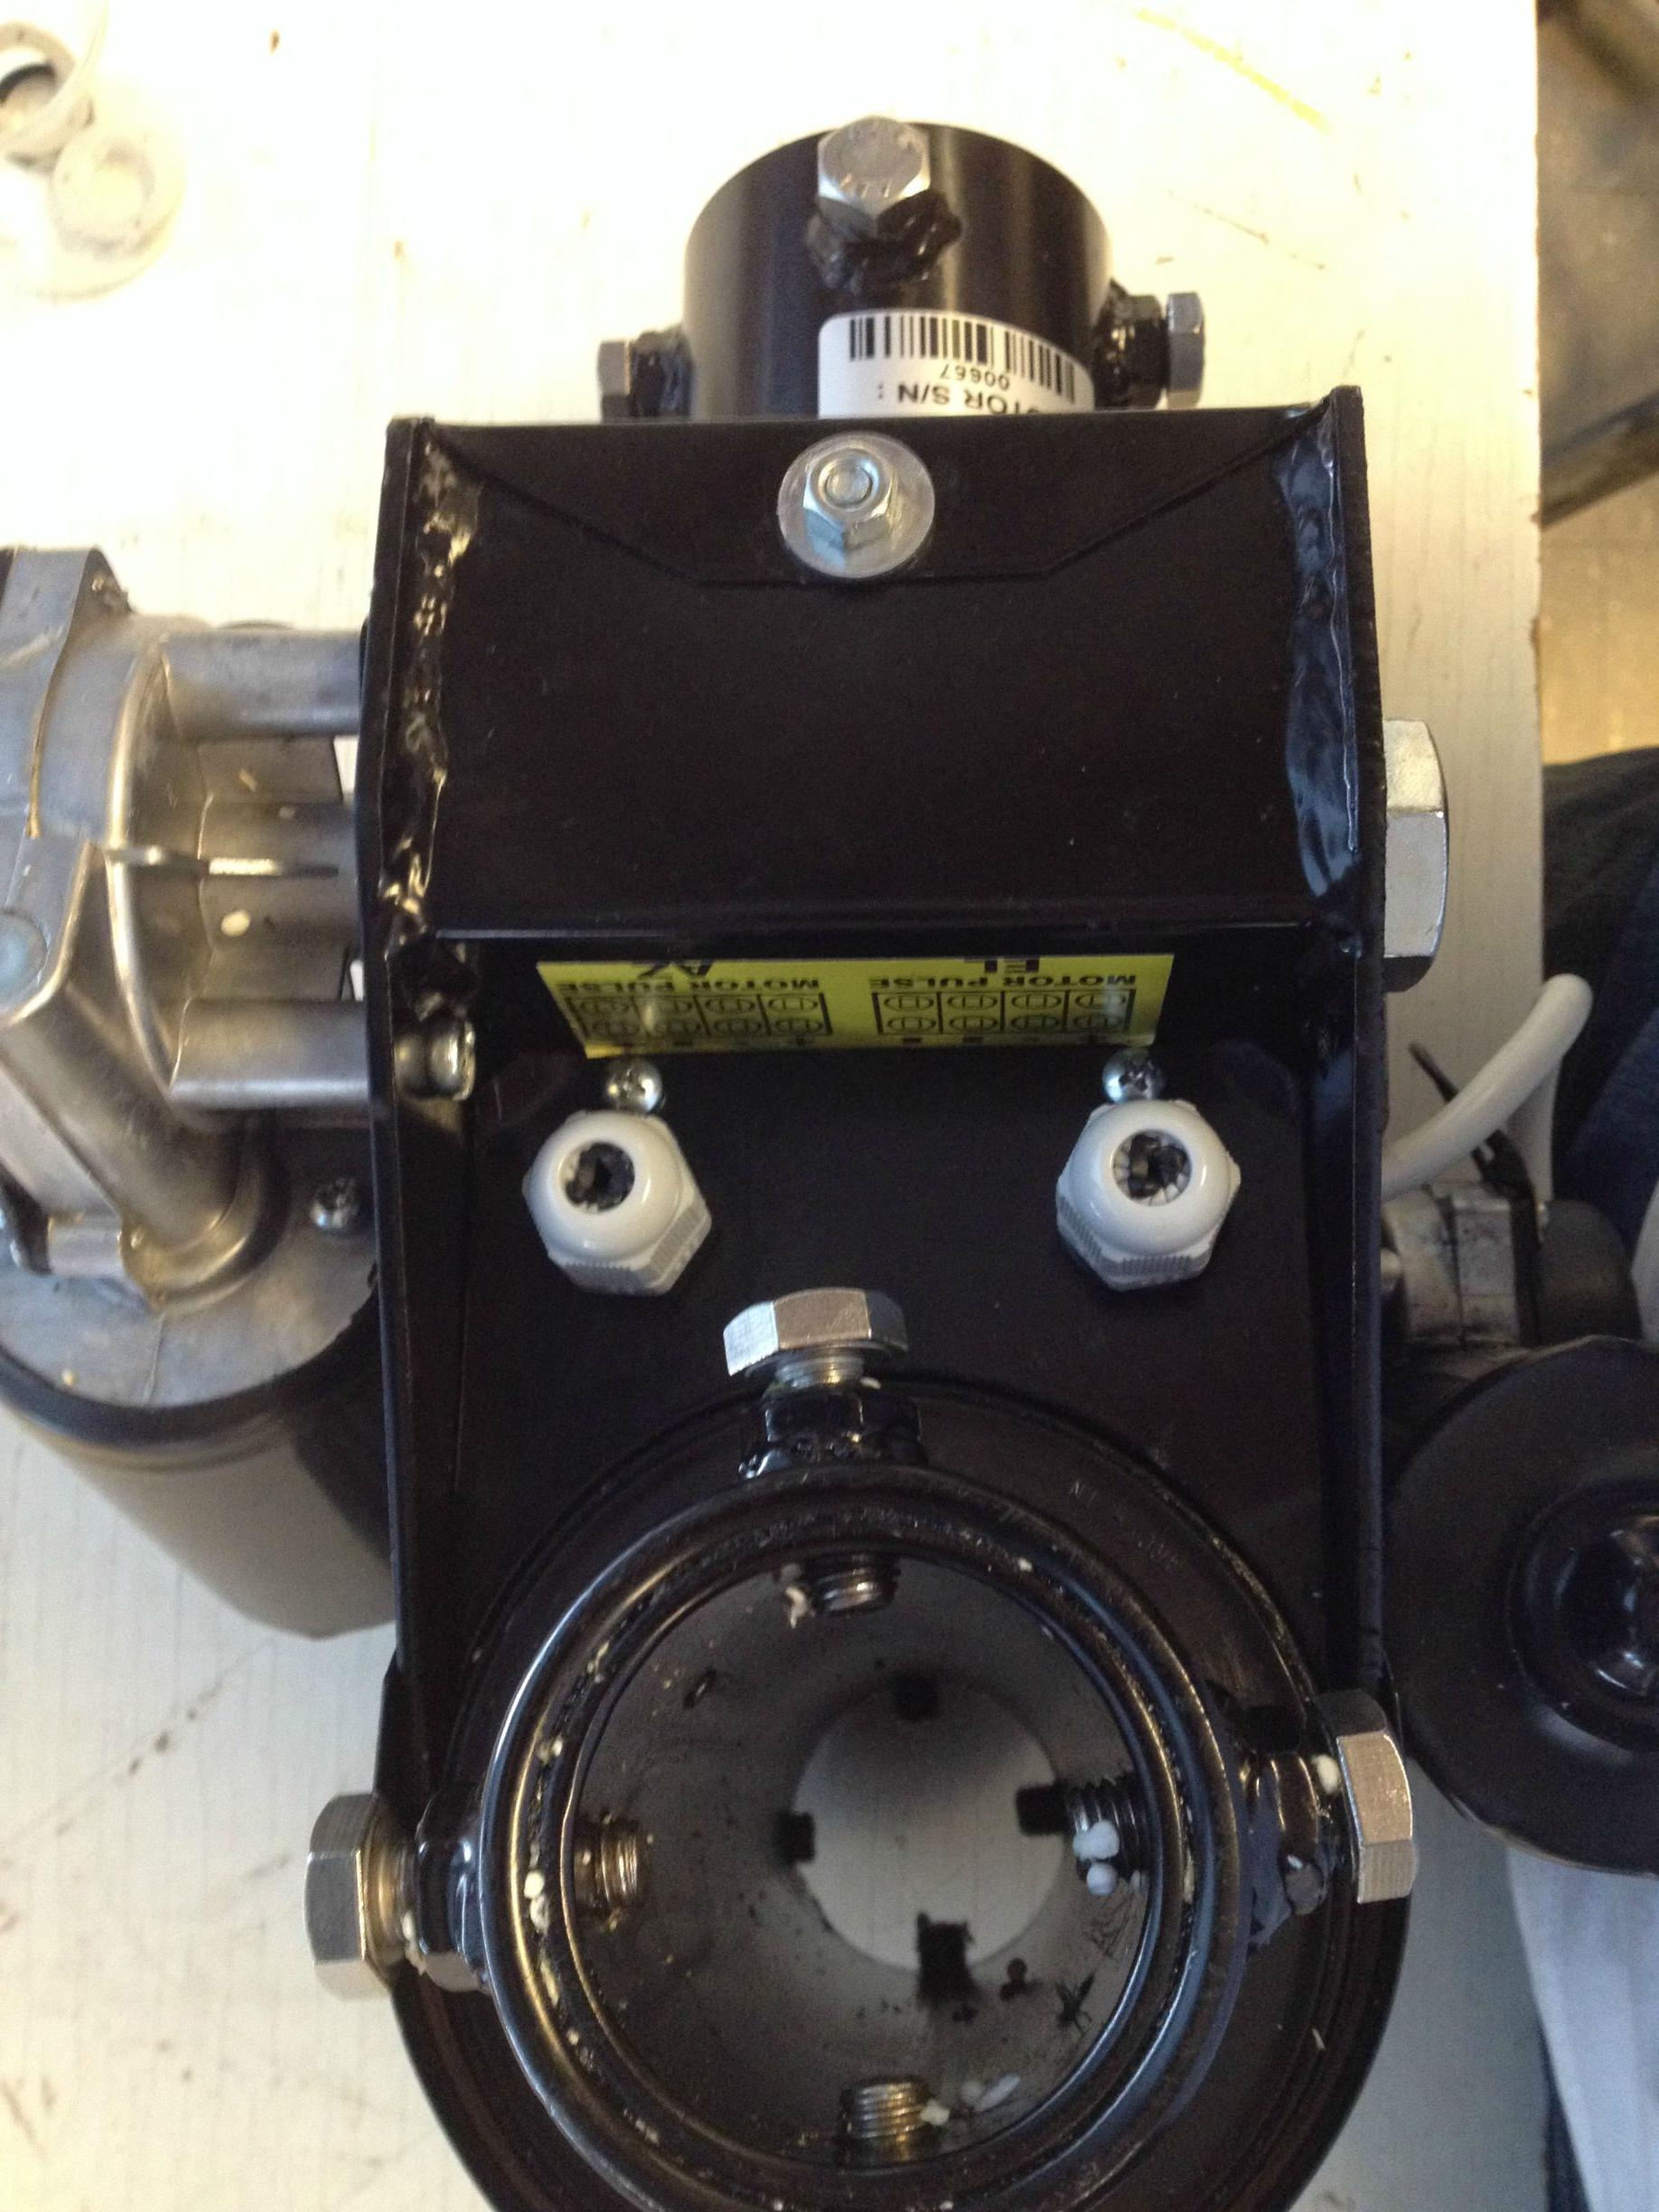
\includegraphics[scale=0.10]{wiring/01.jpeg}
\end{center}

First, unscrew/remove the two waterproof outlets using the adjustable wrench and unscrew the two screws on the plate.

\begin{center}
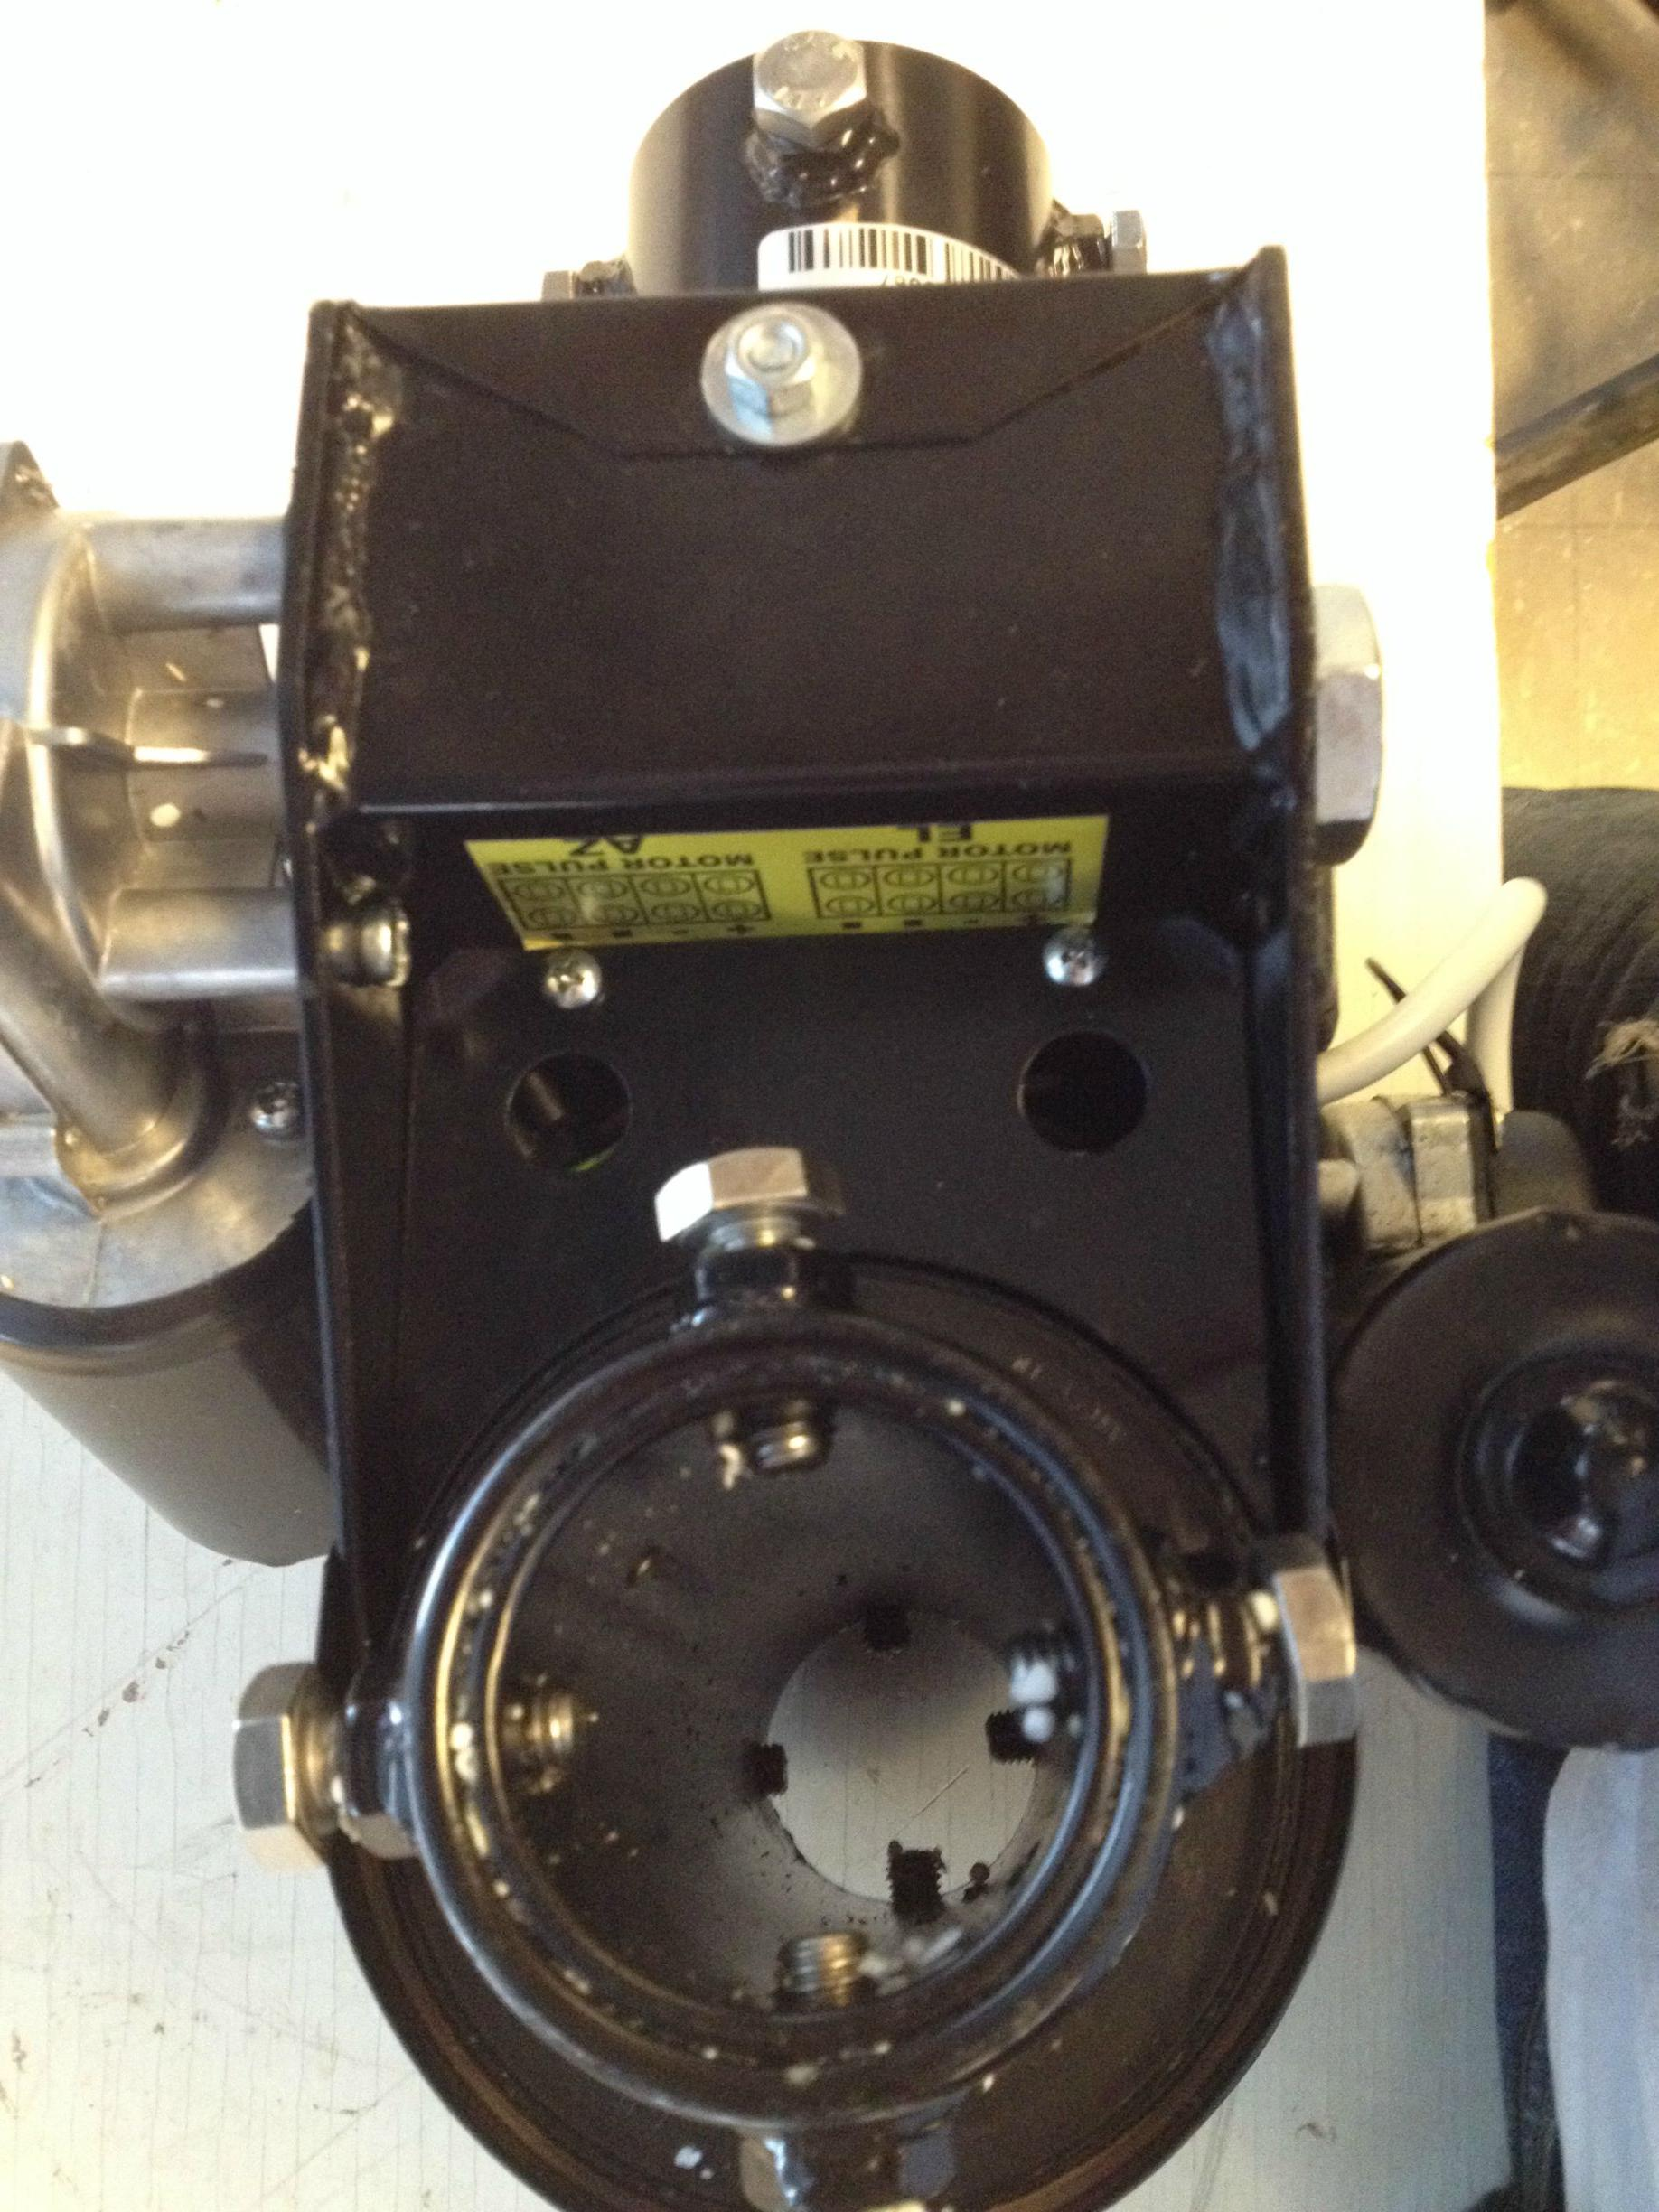
\includegraphics[scale=0.10]{wiring/02.jpeg}

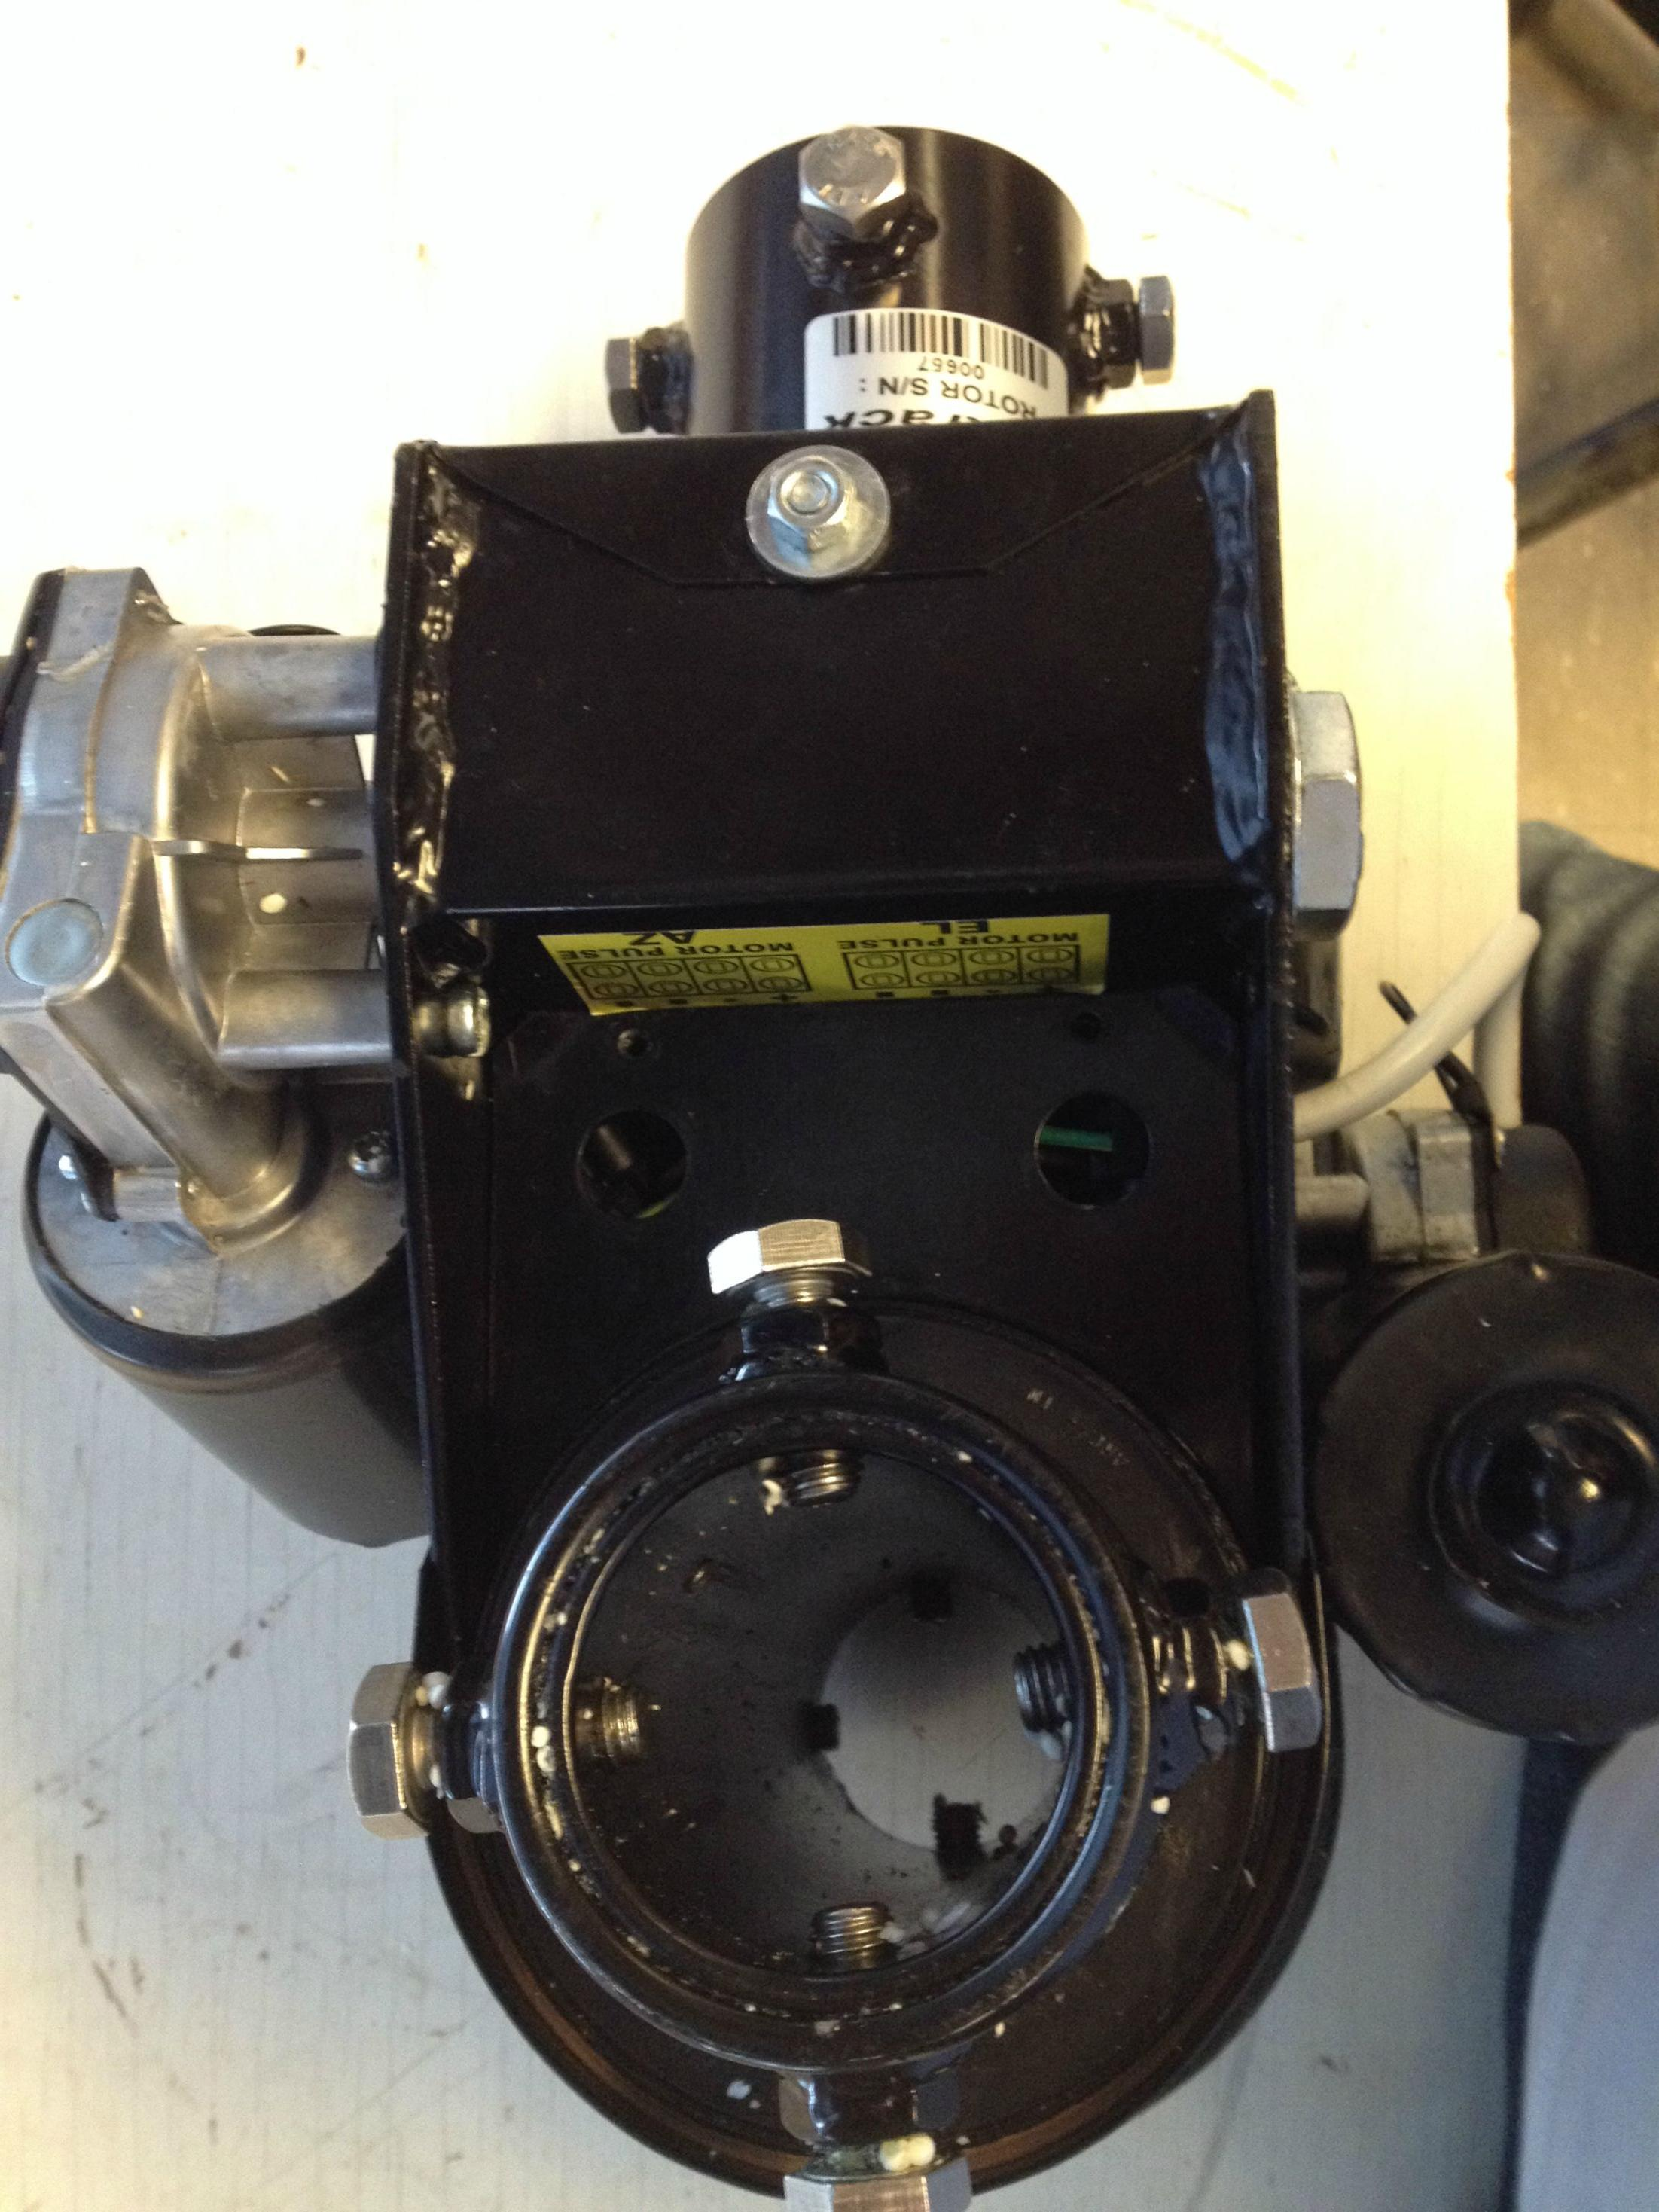
\includegraphics[scale=0.10]{wiring/03.jpeg}
\end{center}


Note that the edge of the plate may be painted over, so use a utility knife to edge the plate. The first time you remove the plate, it may be difficult, so, using the back of a screwdriver, tap around the corners of the plate to loosen it. \\
Using a screwdriver (or some other means of leverage), insert one end into a hole left from unscrewing the waterproof outlet, and carefully pry off the plate. This may take some time since the plate has a tight fit initially.


\begin{center}
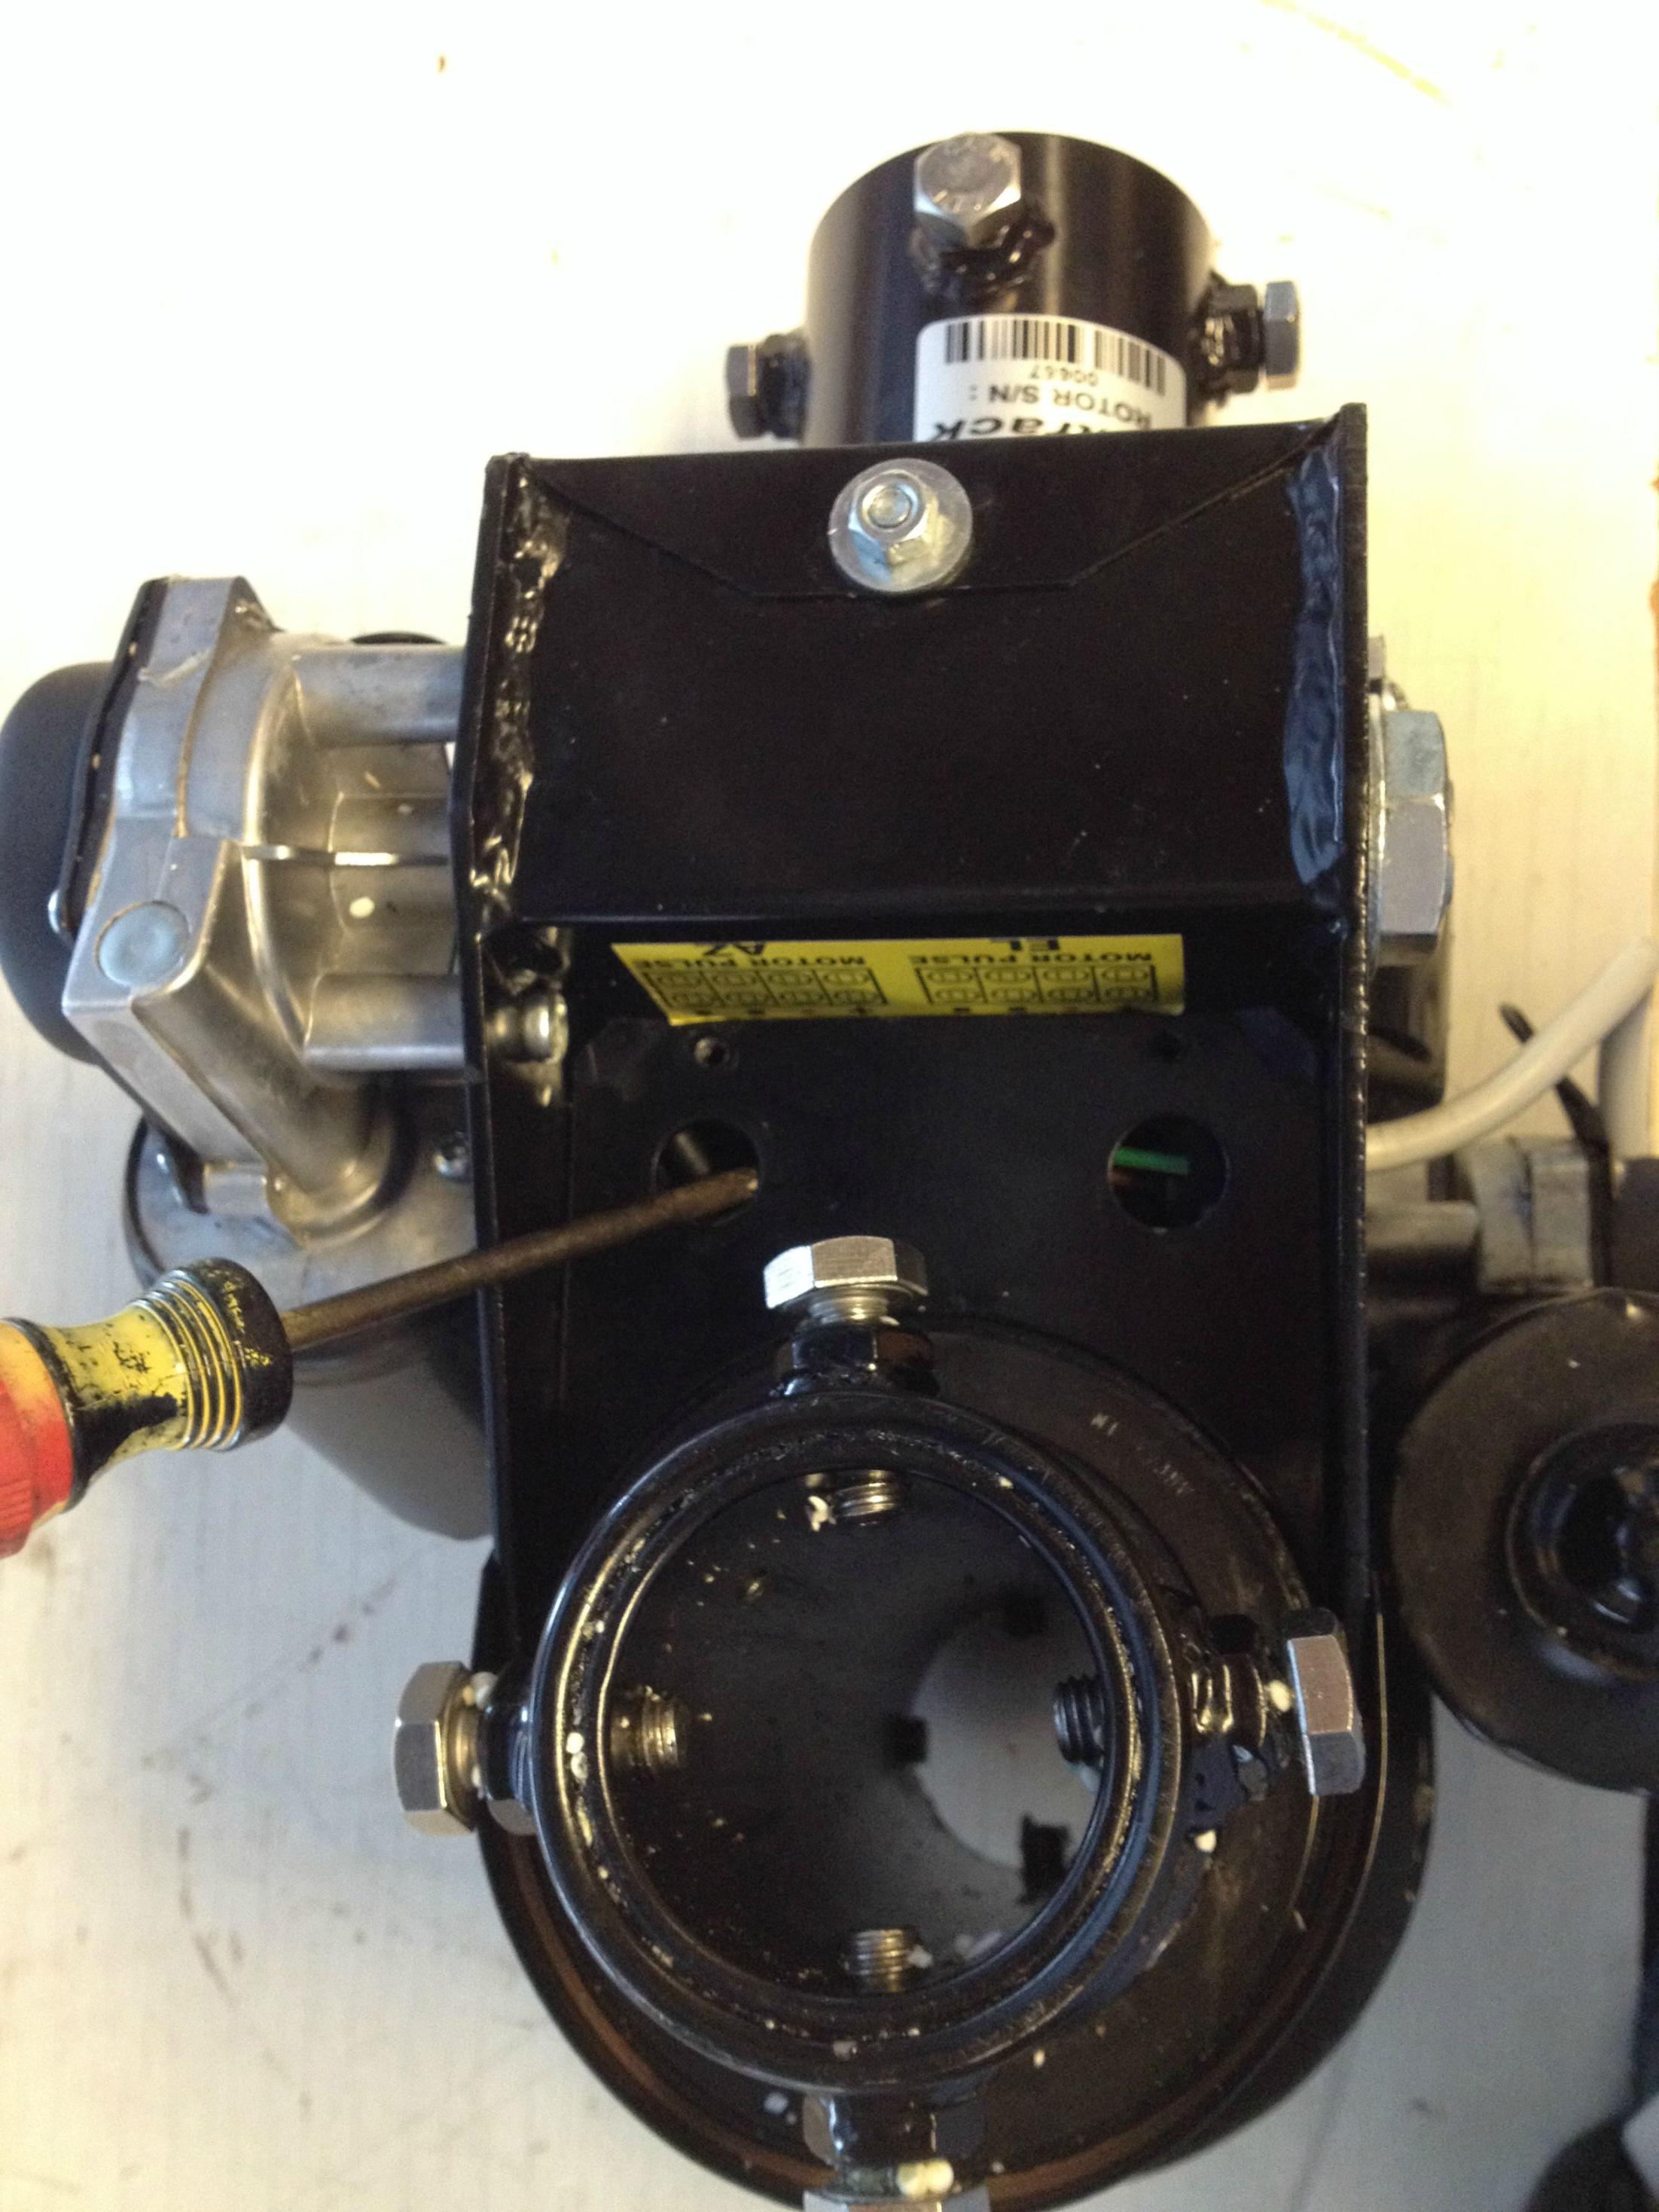
\includegraphics[scale=0.10]{wiring/04.jpeg}
\end{center}


Underneath the plate are two wiring terminals, one for AZ and one for EL. (See the sticker on the rotor to determine which terminal corresponds to AZ and which corresponds to EL).


\begin{center}
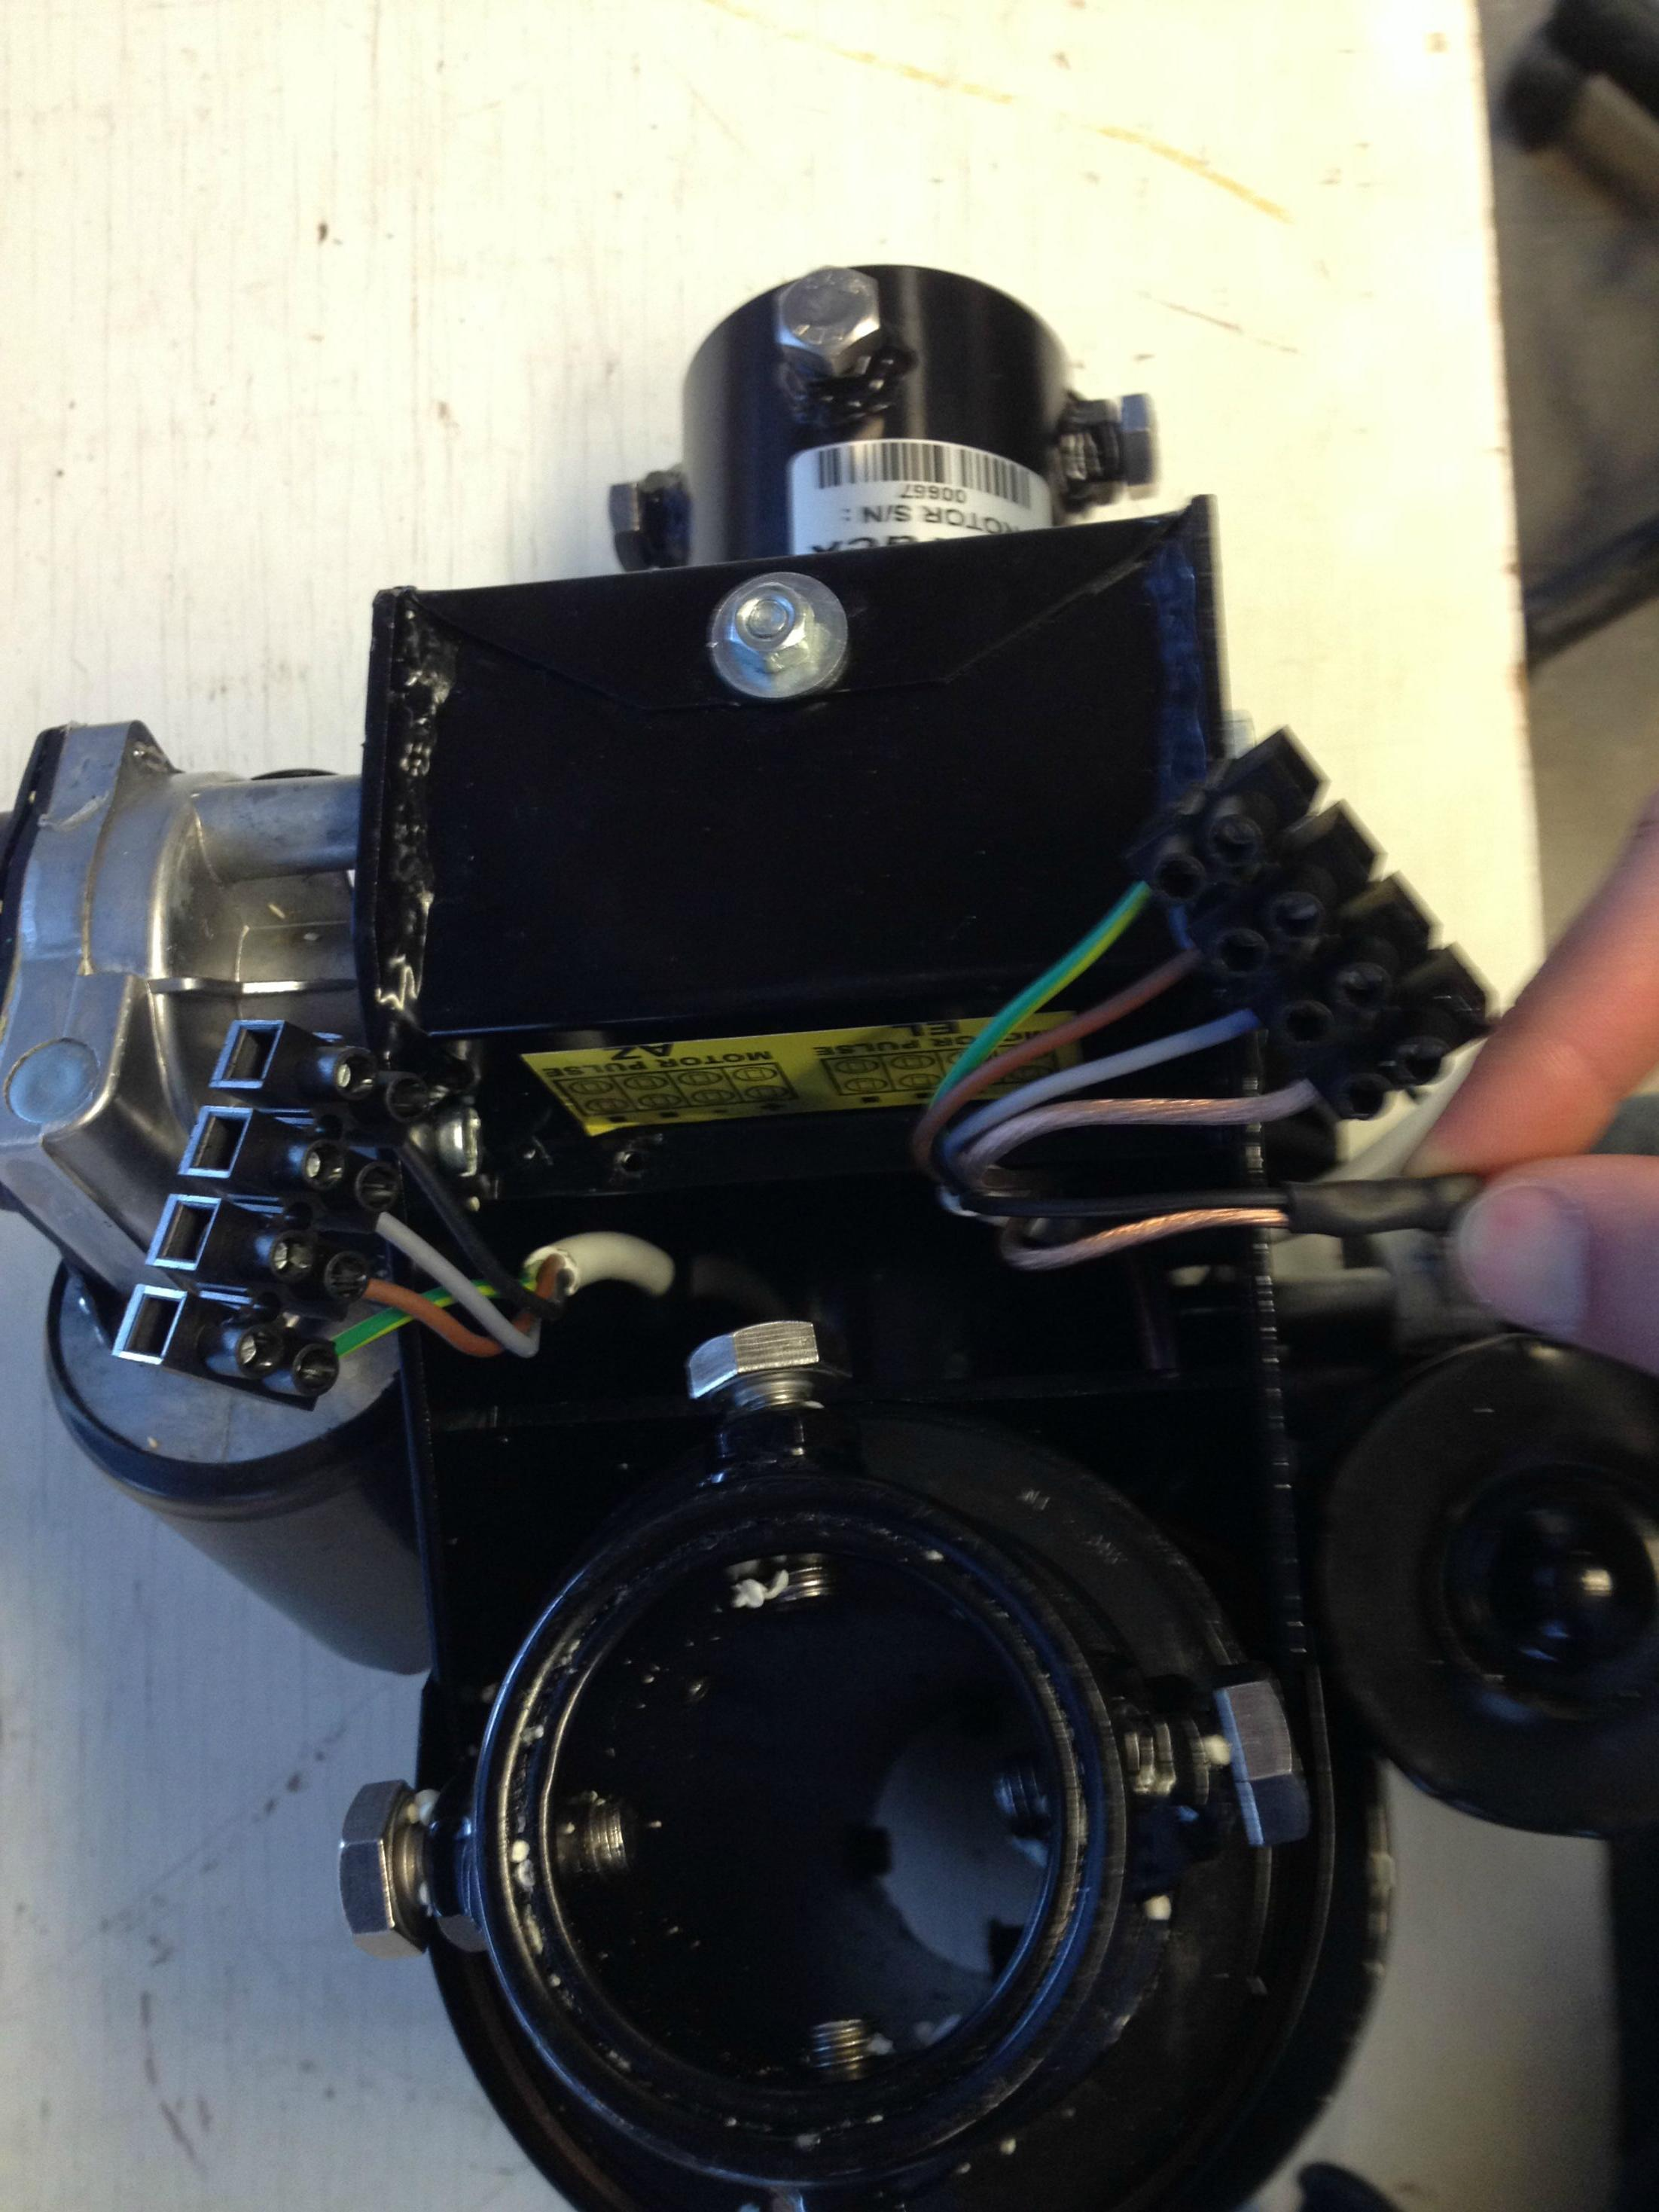
\includegraphics[scale=0.10]{wiring/05.jpeg}
\end{center}


For testing purposes, a set of test cables were made, approx. 75 cm long. (Later, these wires were replaced with more permanent ones to fit our mounting strategy). Our test cables consisted of four cables, each cable containing two wires, so there were two cables per terminal, or four wires per terminal. The ends of the wires were stripped and tinned.

\begin{center}
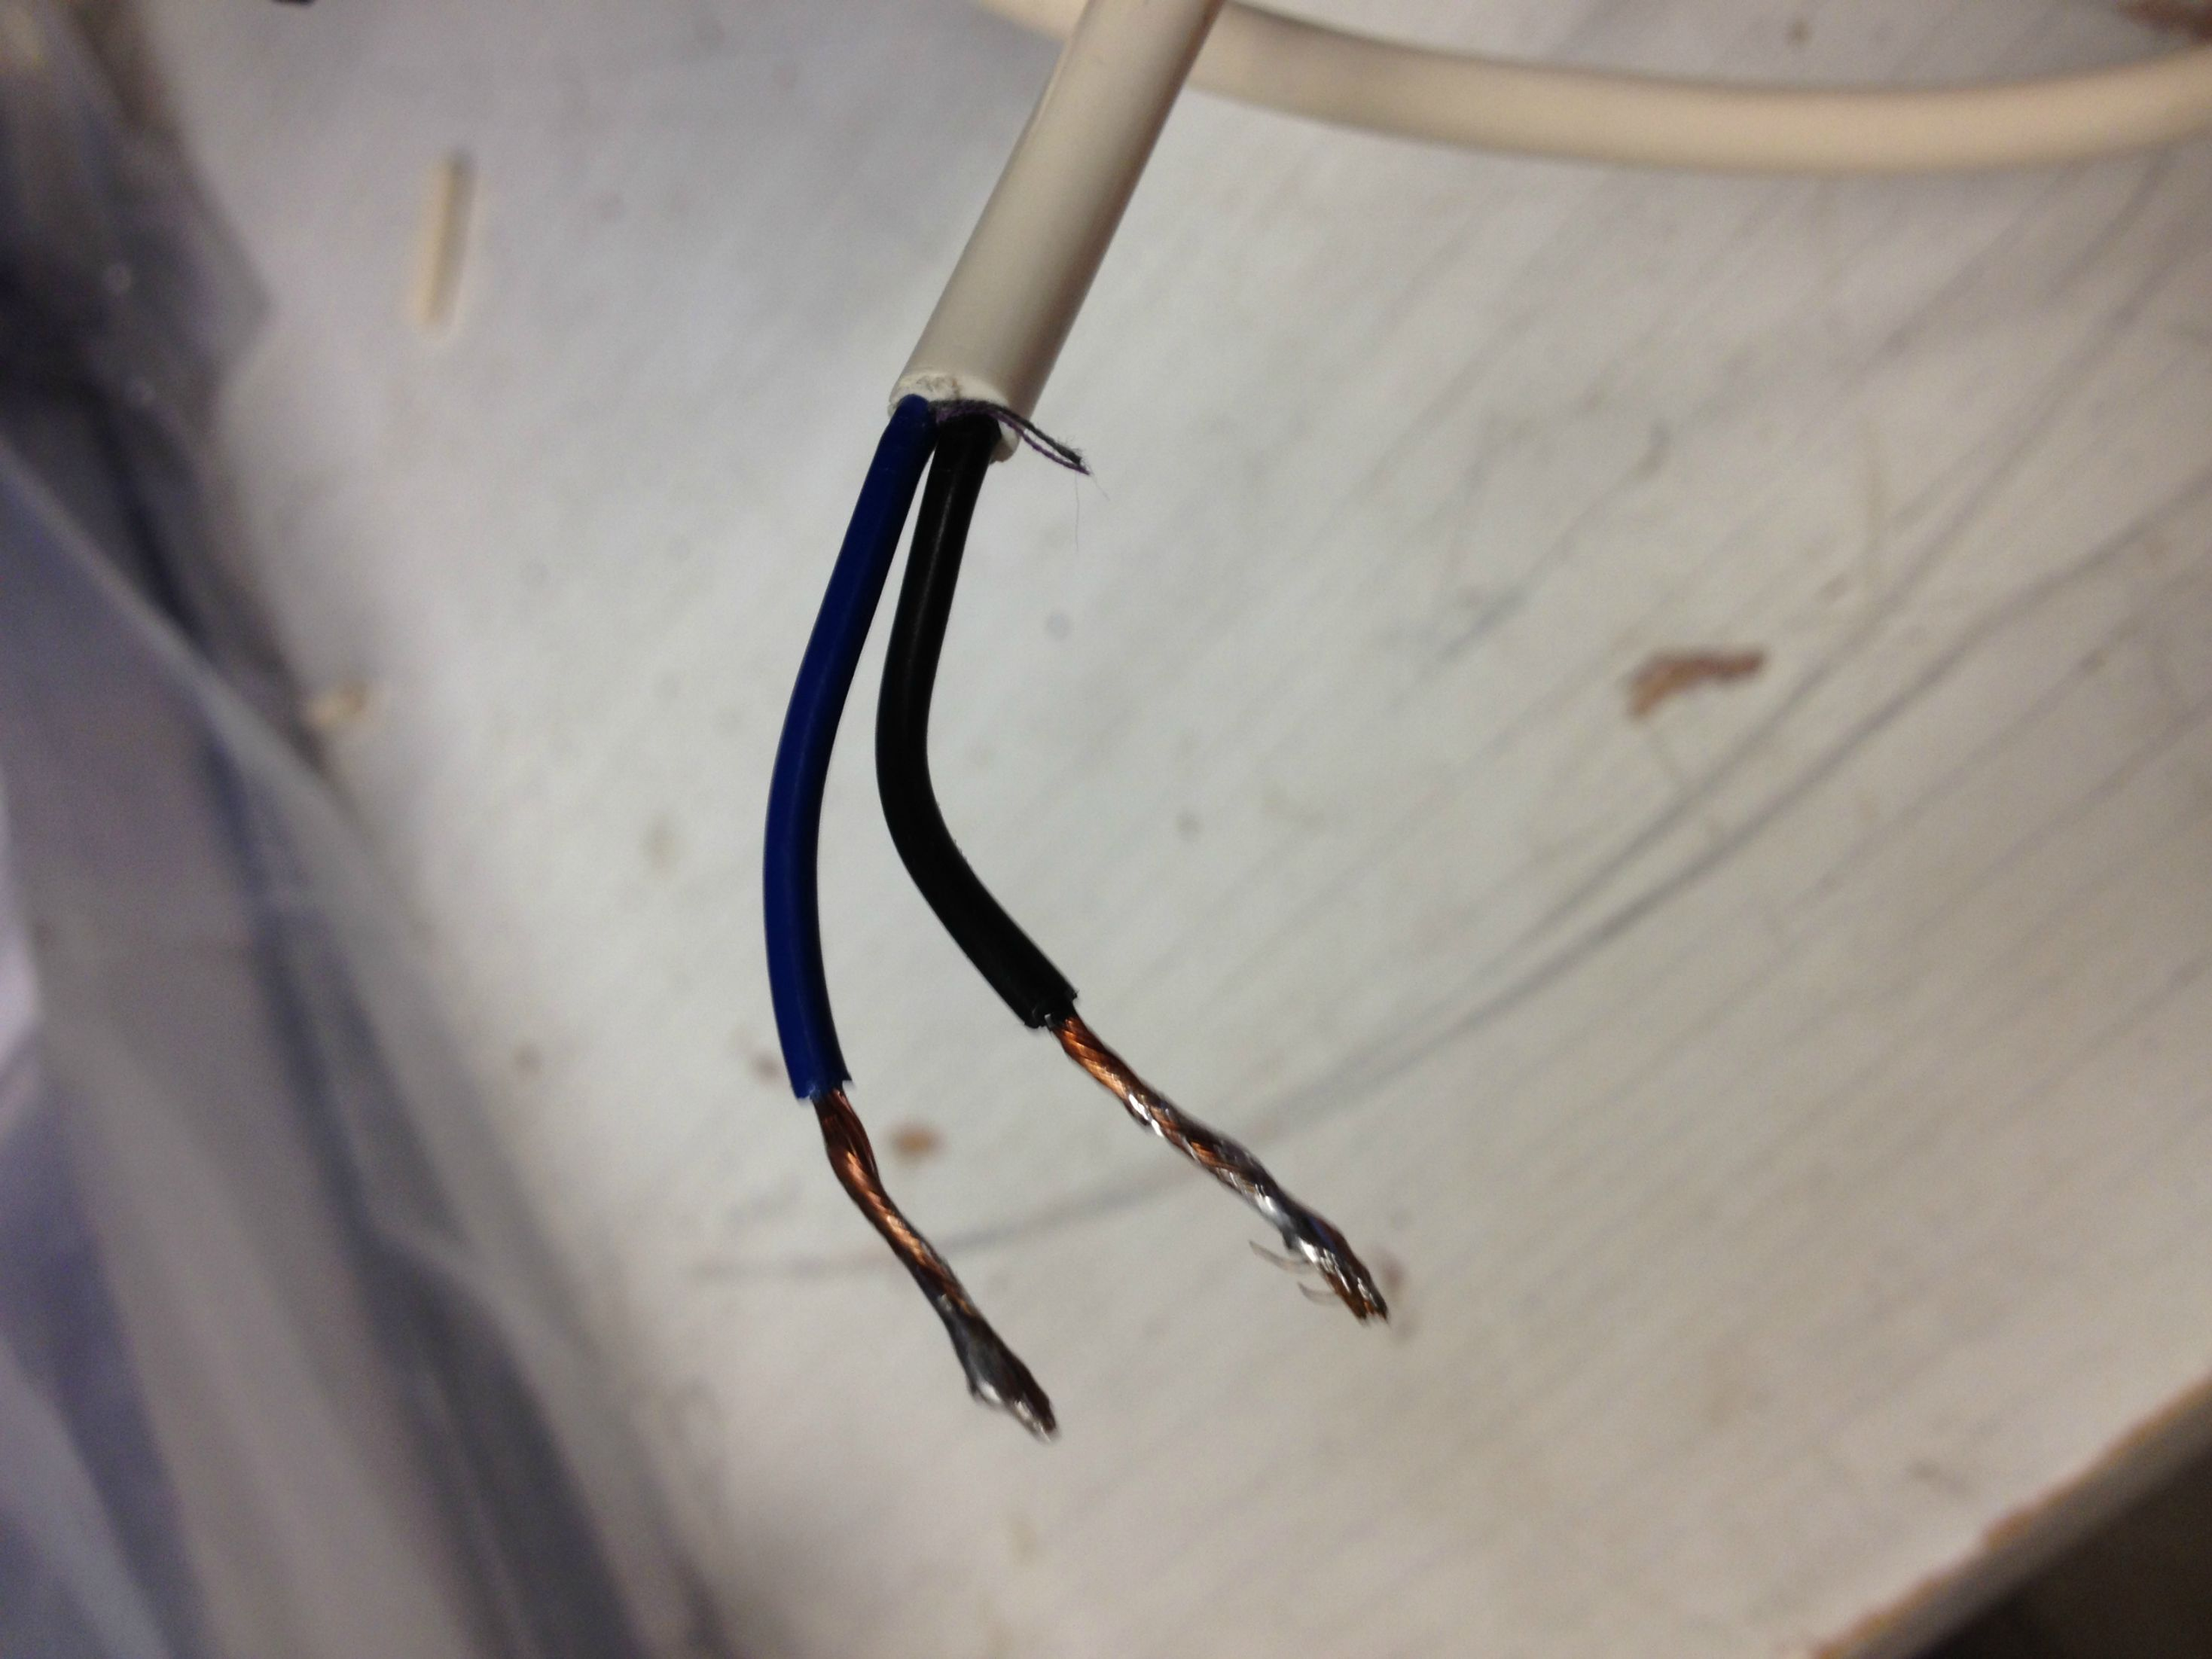
\includegraphics[scale=0.10]{wiring/06.jpeg}
\end{center}

The ends of the wires were secured in their respective rotator terminal.

\begin{center}
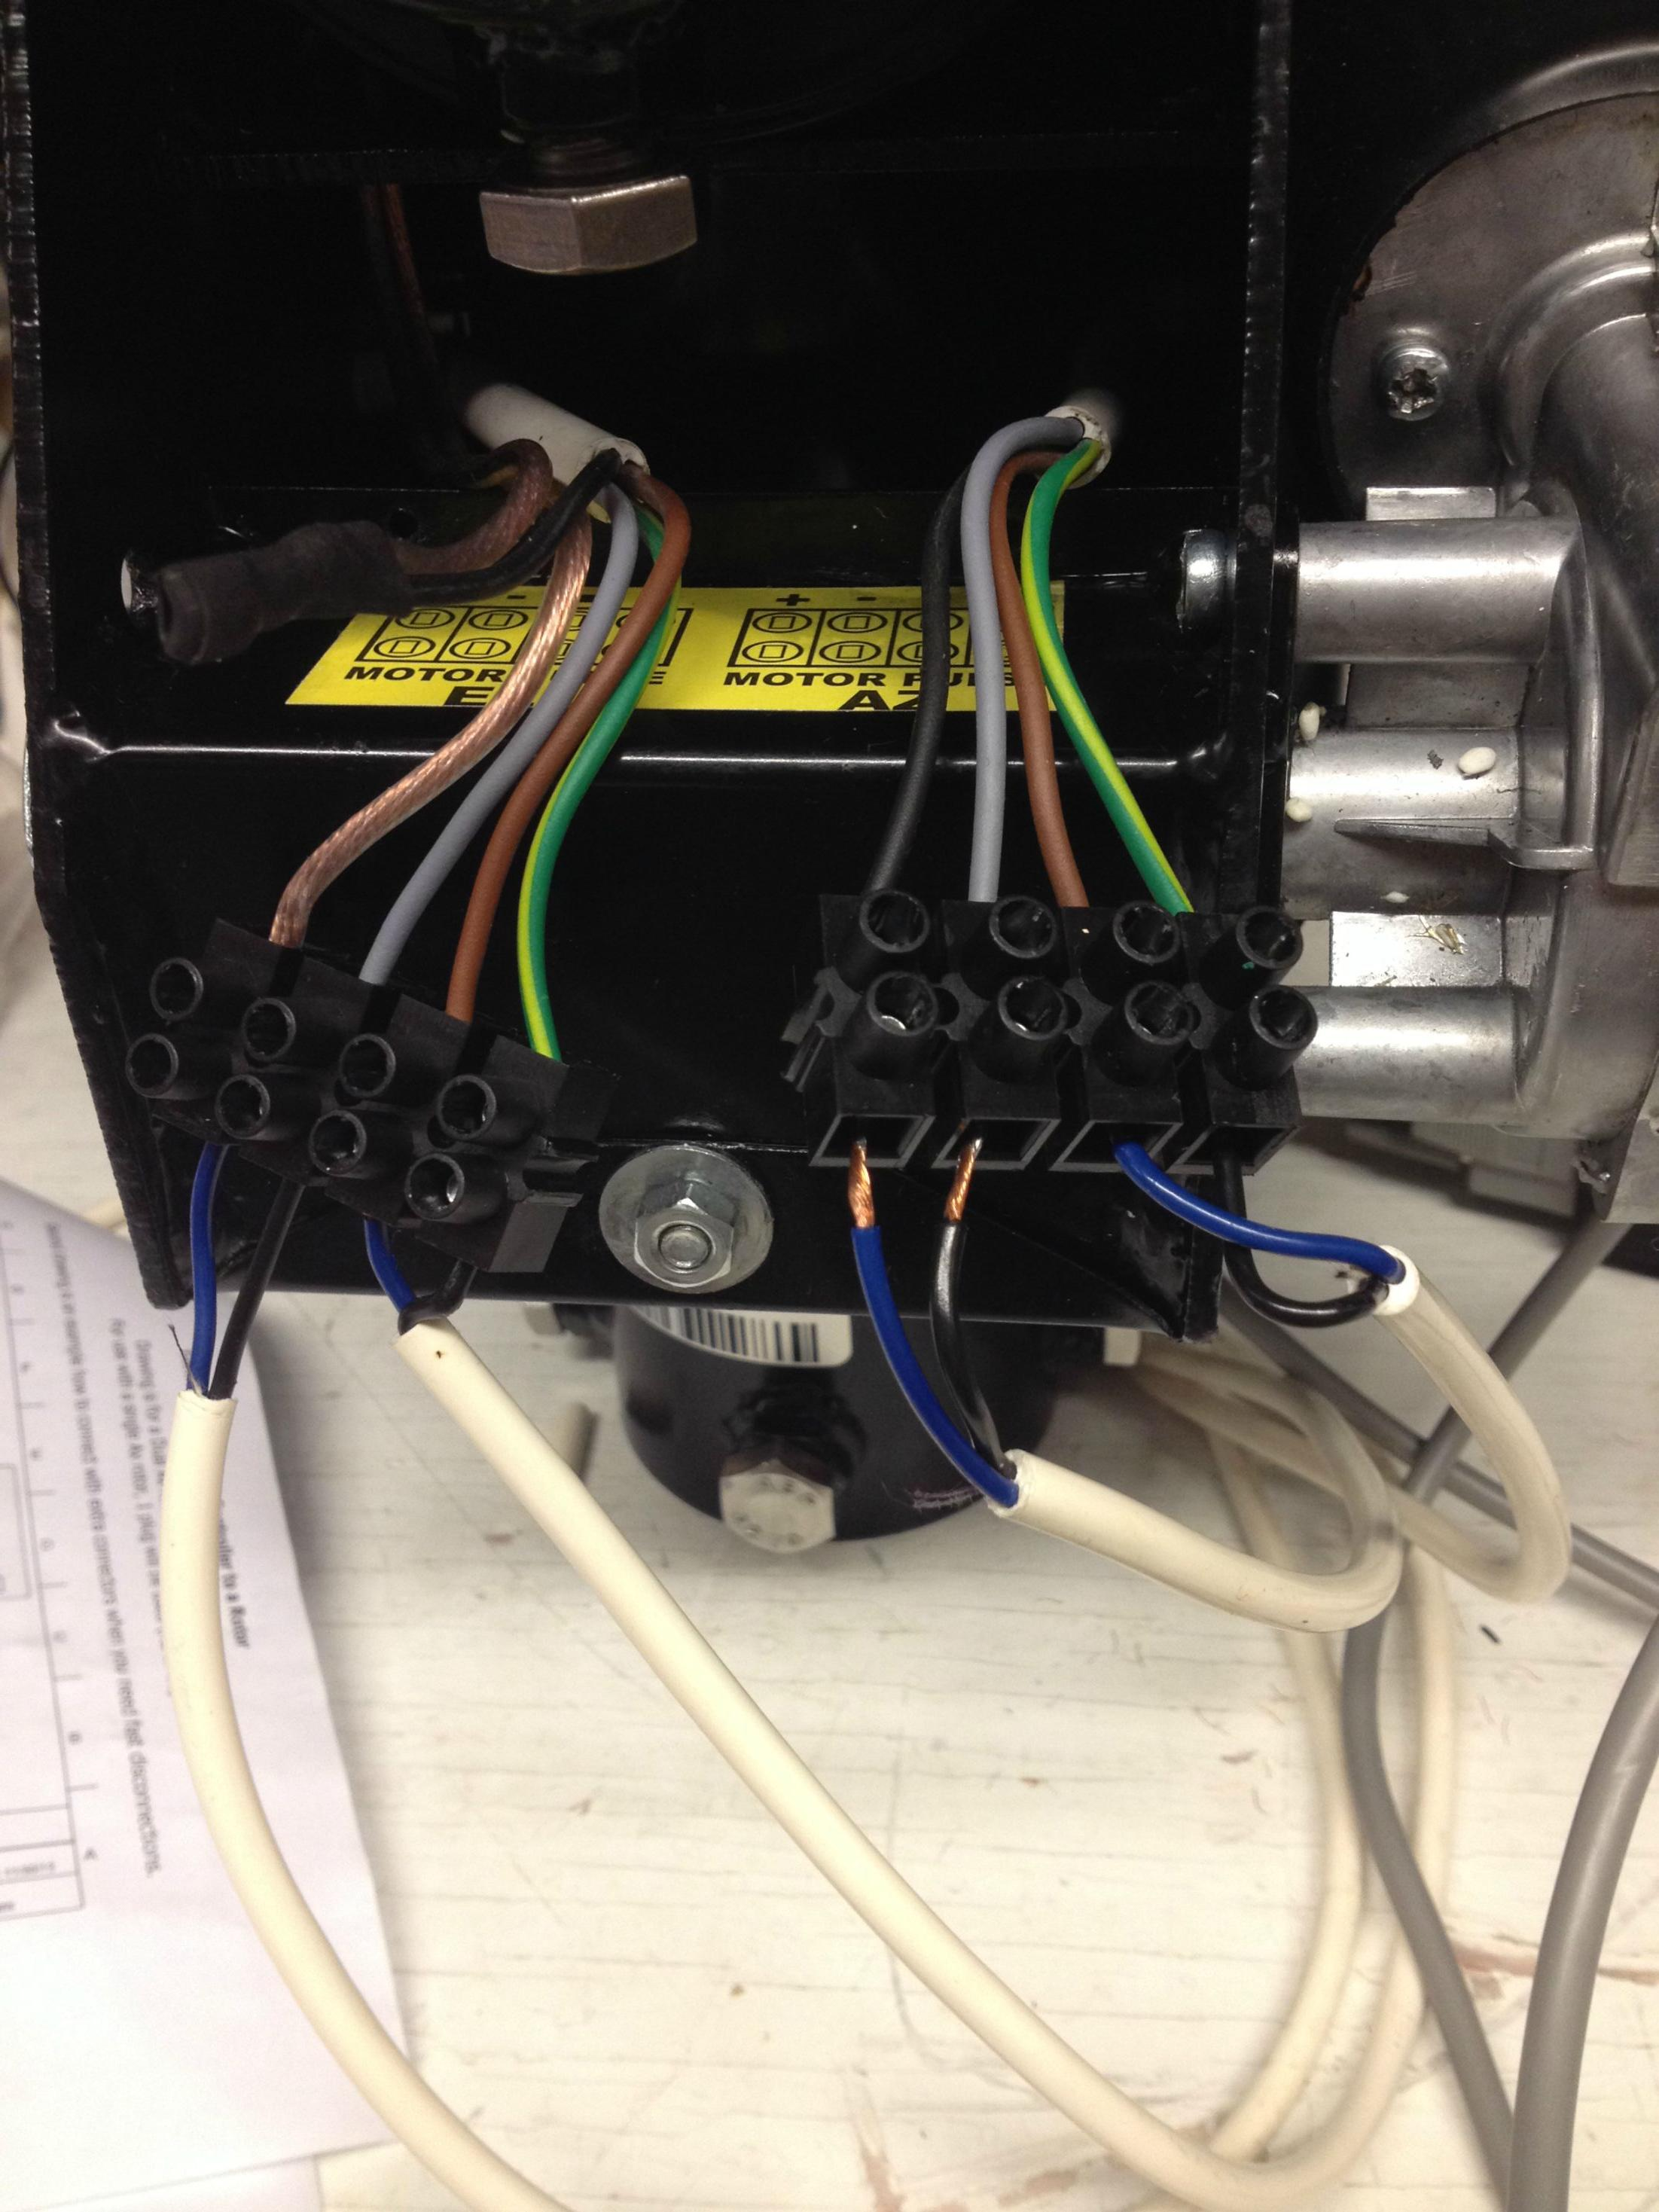
\includegraphics[scale=0.10]{wiring/07.jpeg}
\end{center}

The free end was then soldered to a head which connects to the controller. When doing this, note the order of the wires. On the head, the pins are labeled 1-4, which will correspond sequentially to the wires coming from the terminal. Electrical tape was wrapped around the wire near the connection to ensure each pin and wire were isolated from one another. Stripping a small amount of wire on this end may diminish the need to wrap the connection in electrical tape.

\begin{center}
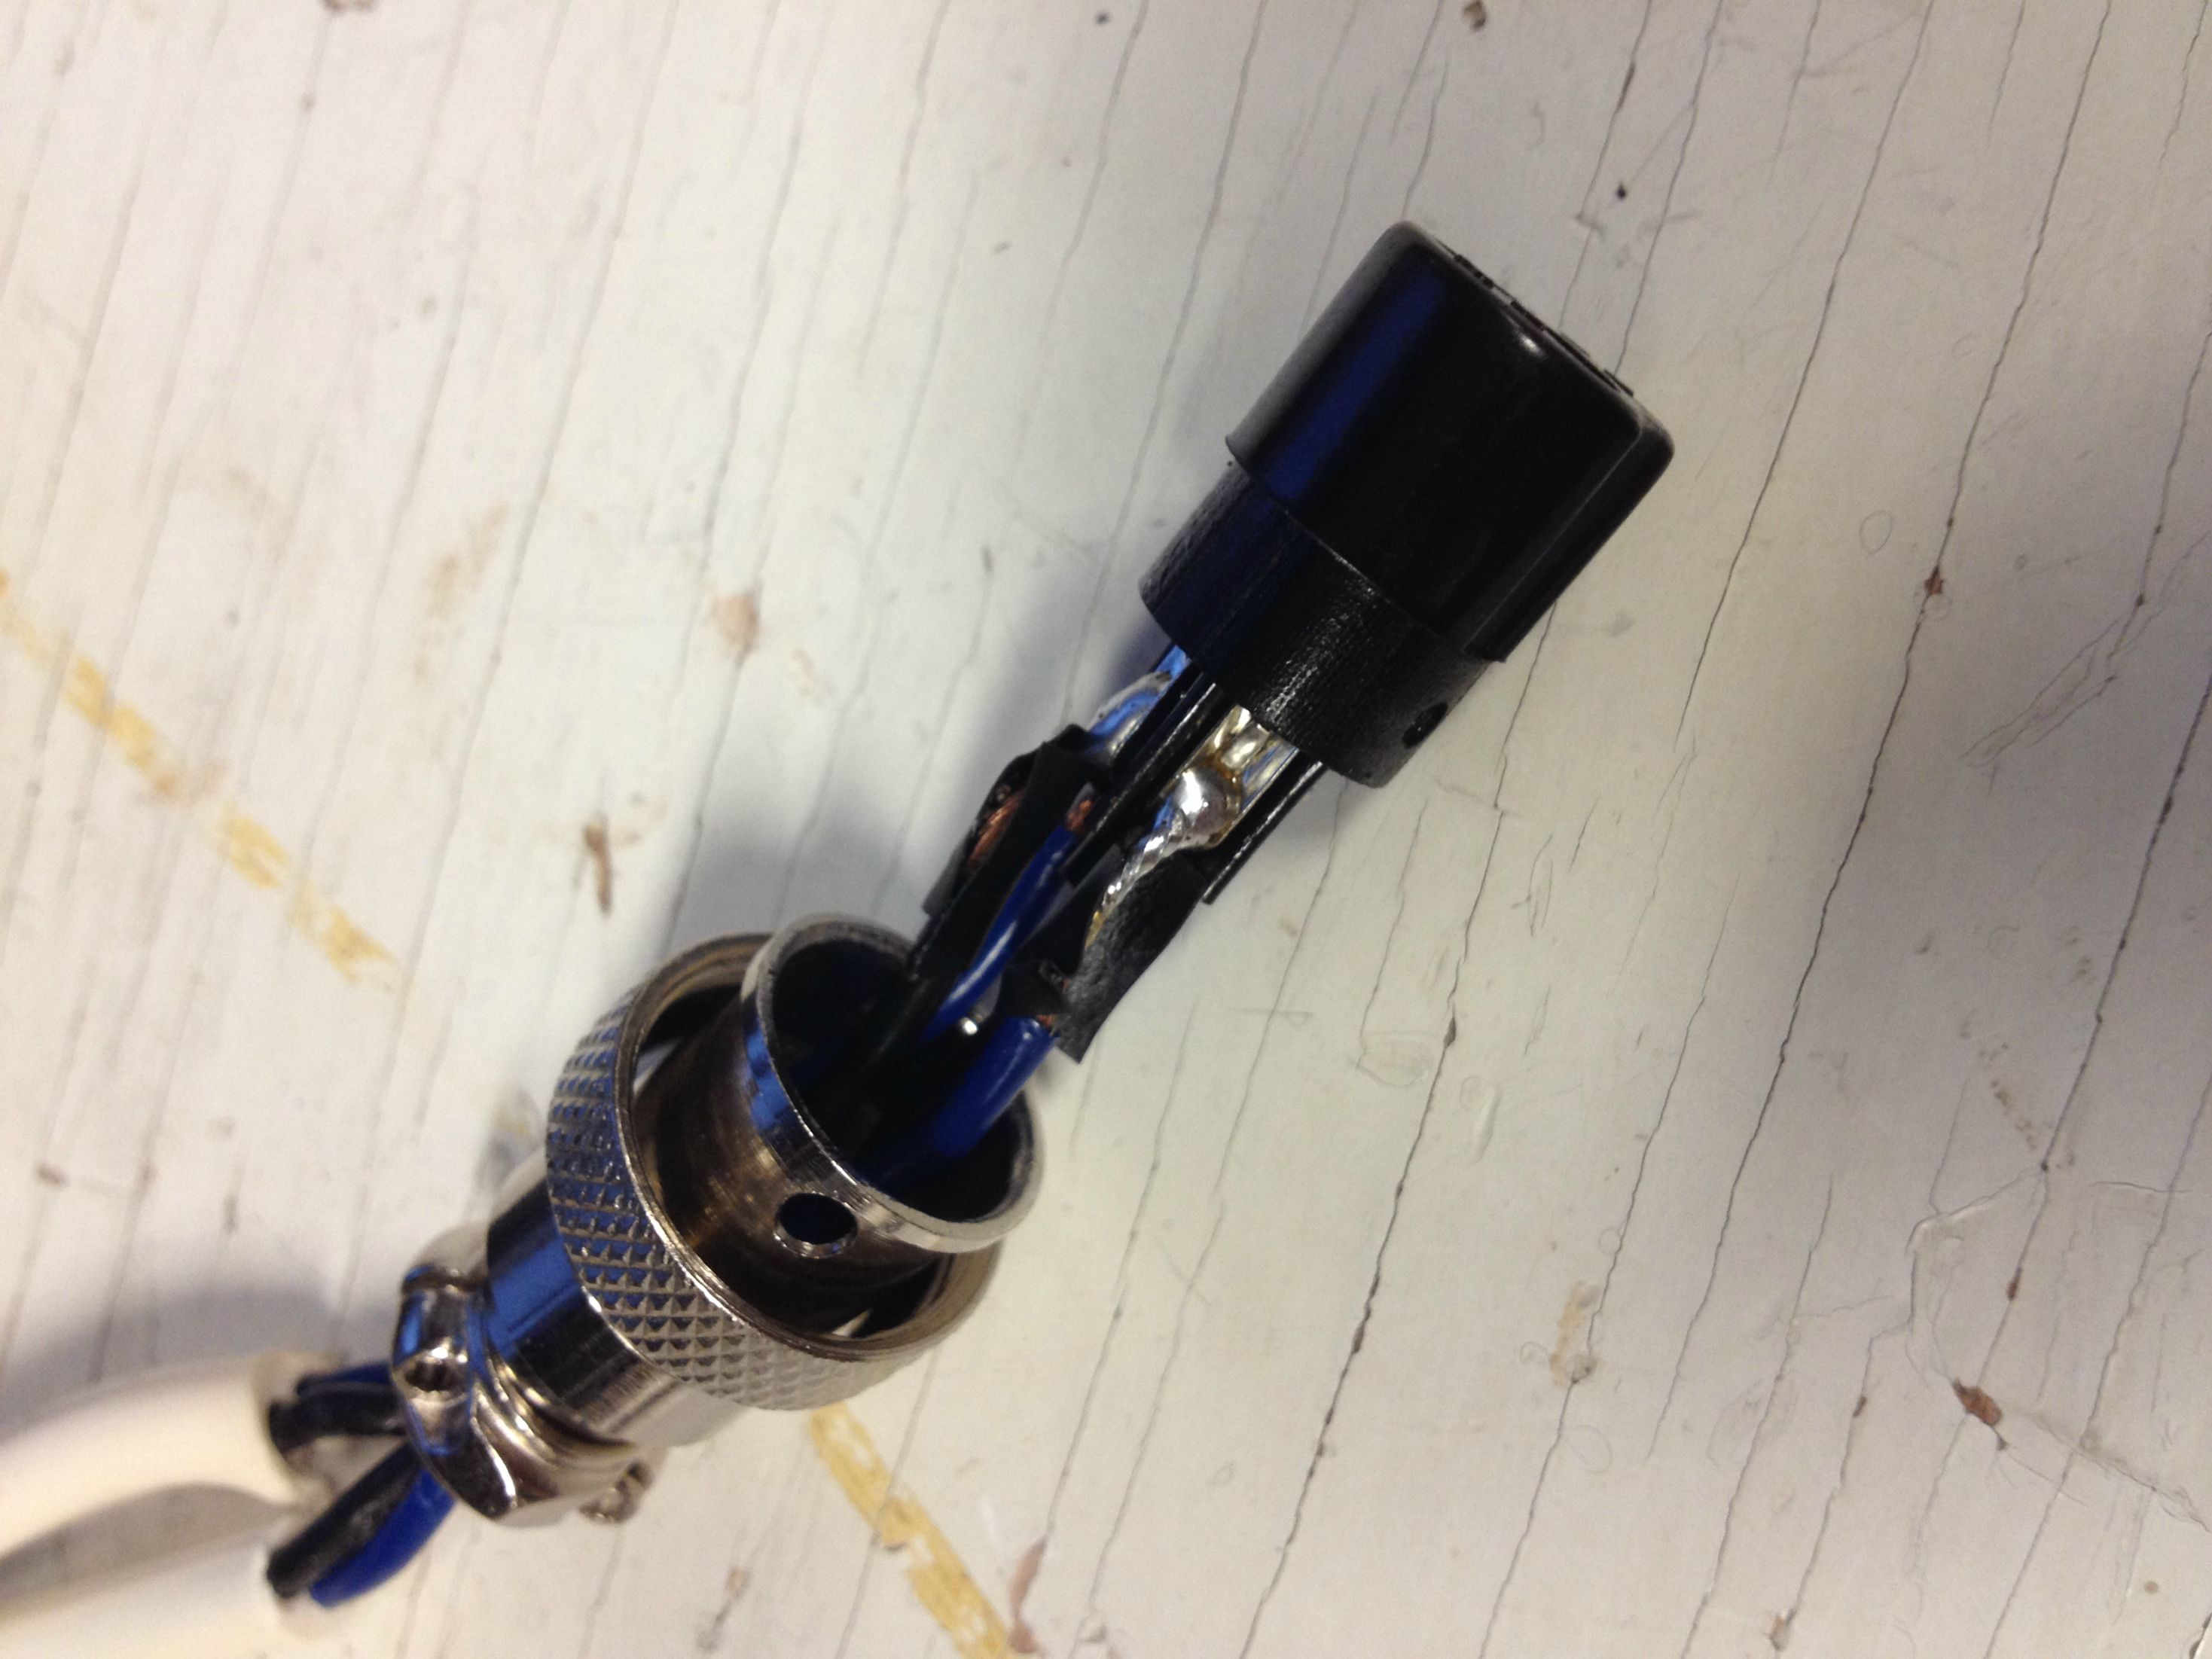
\includegraphics[scale=0.10]{wiring/08.jpeg}
\end{center}

The head was re-assembled and connected to the controller.

\begin{center}
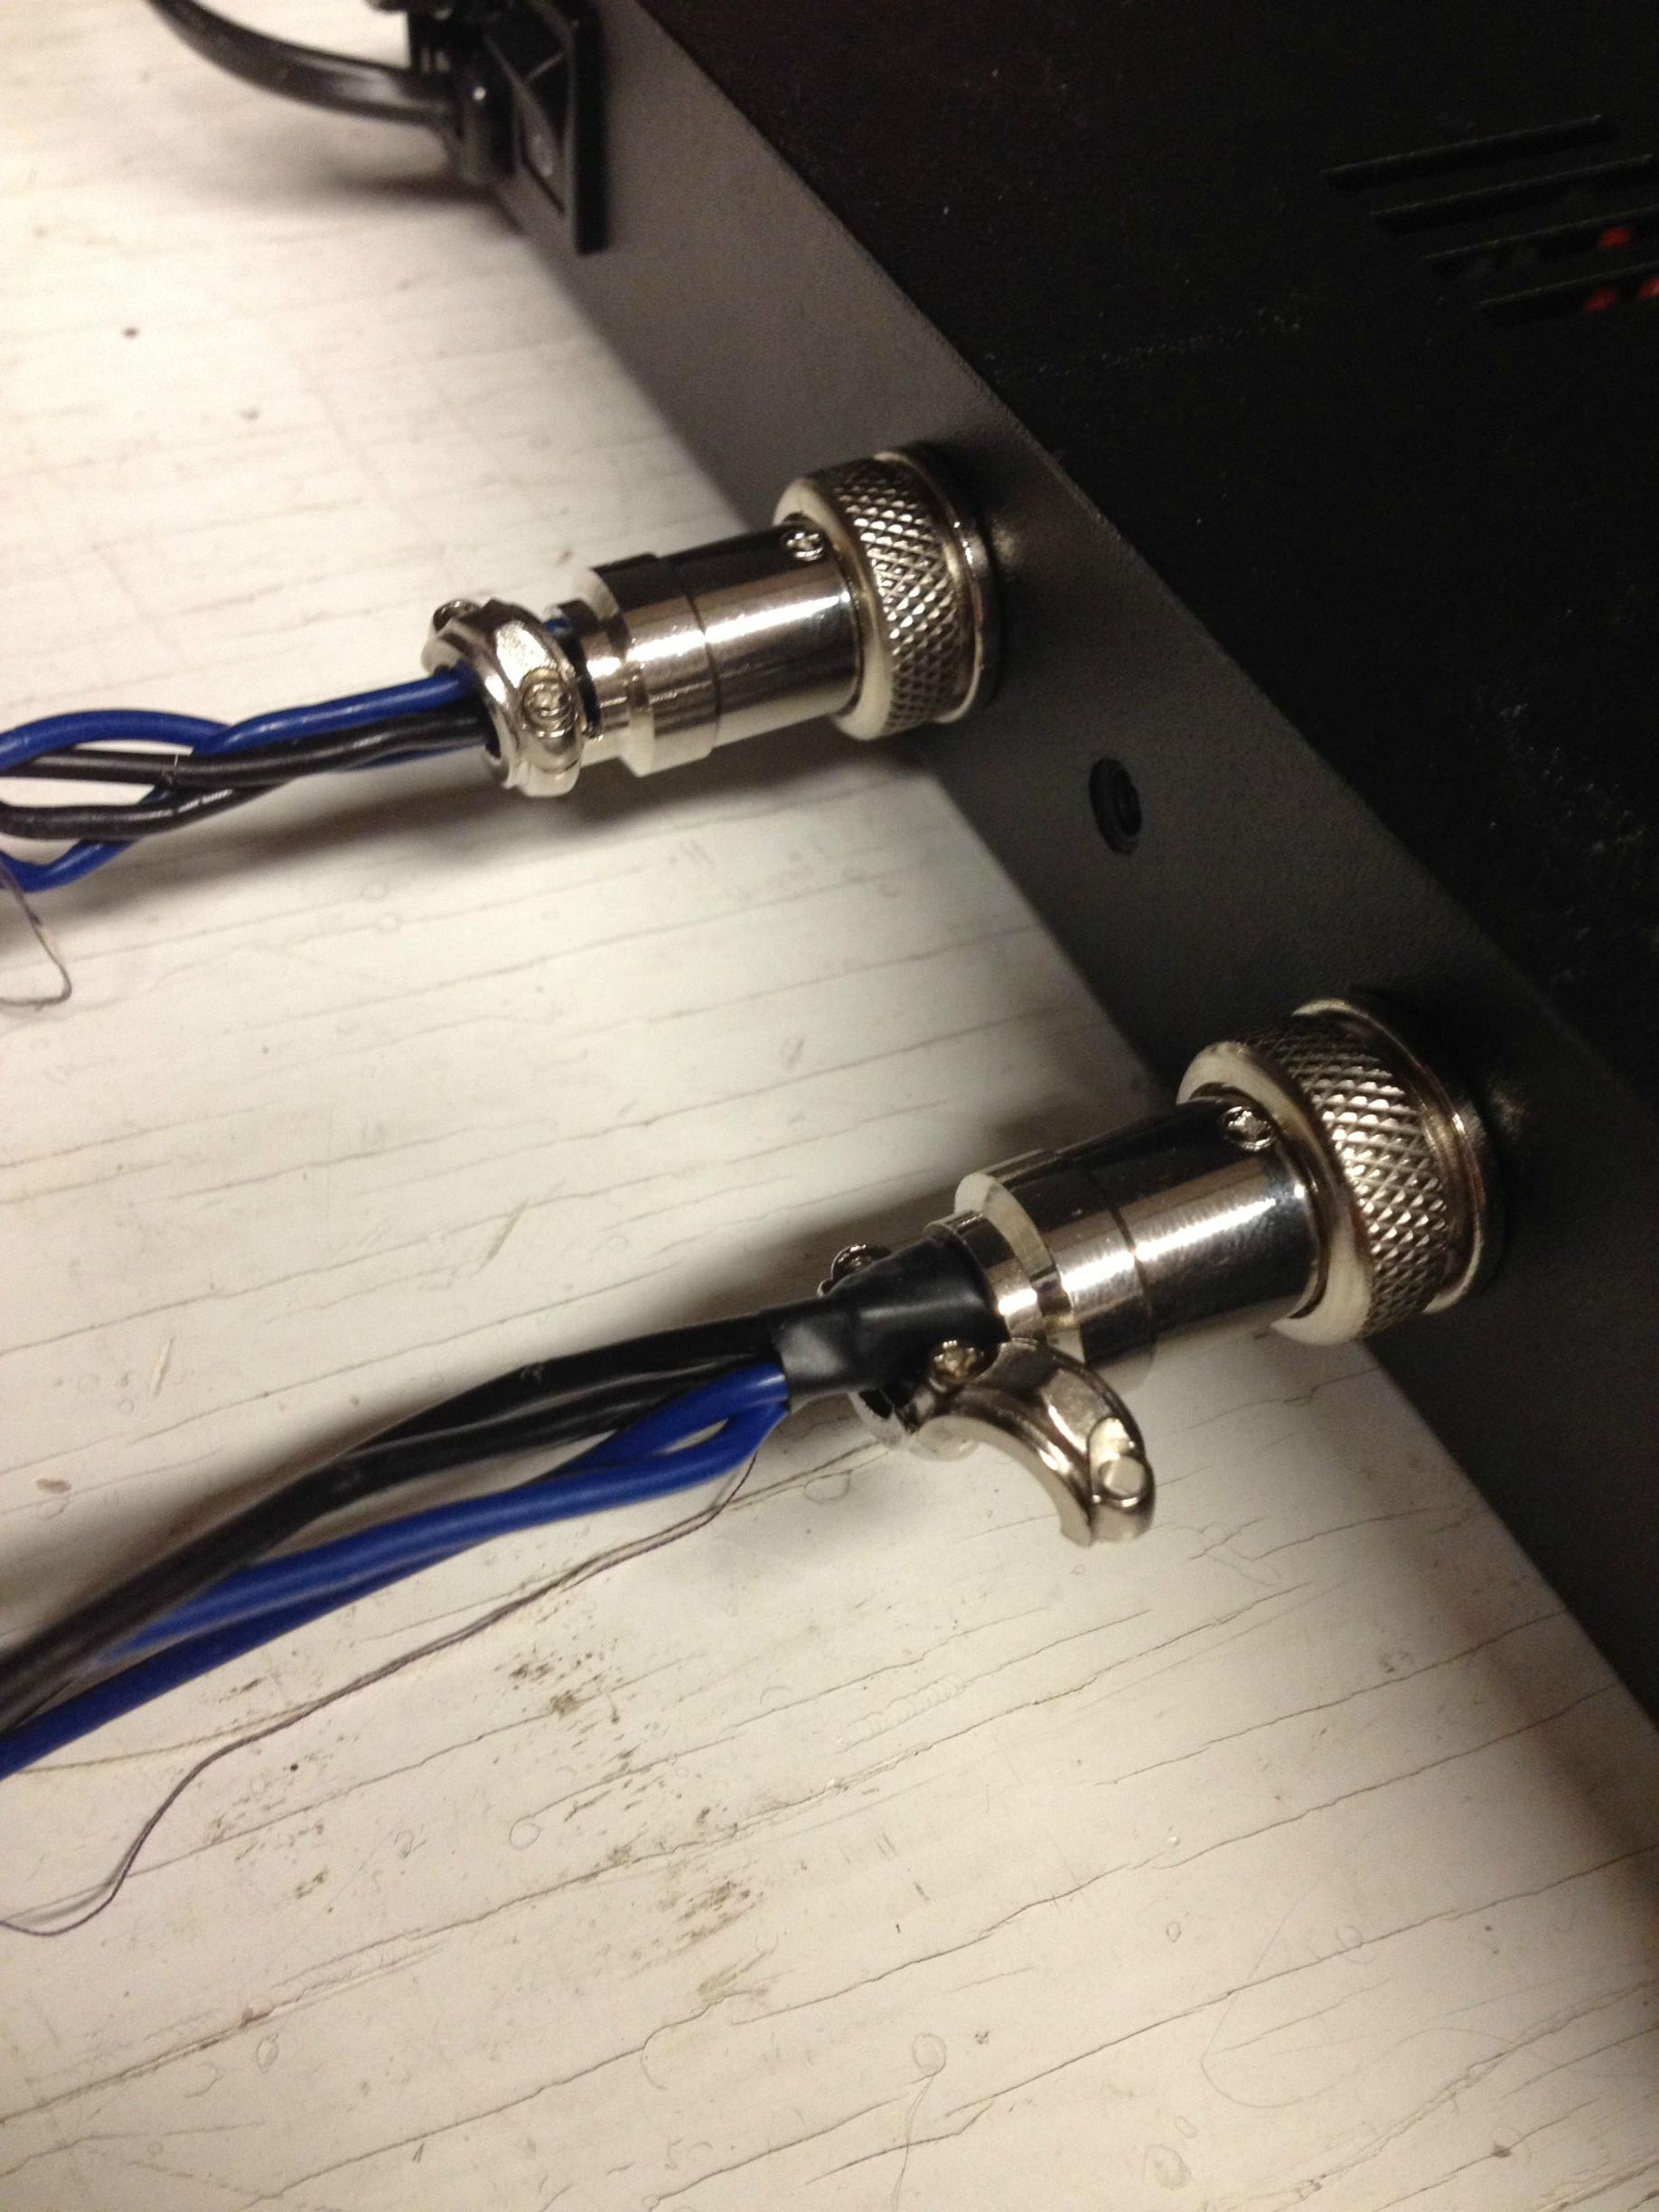
\includegraphics[scale=0.10]{wiring/09.jpeg}
\end{center}

Once everything was secure and connected, the power supply and controller were turned on, with the mouse attached to the controller.

\begin{center}
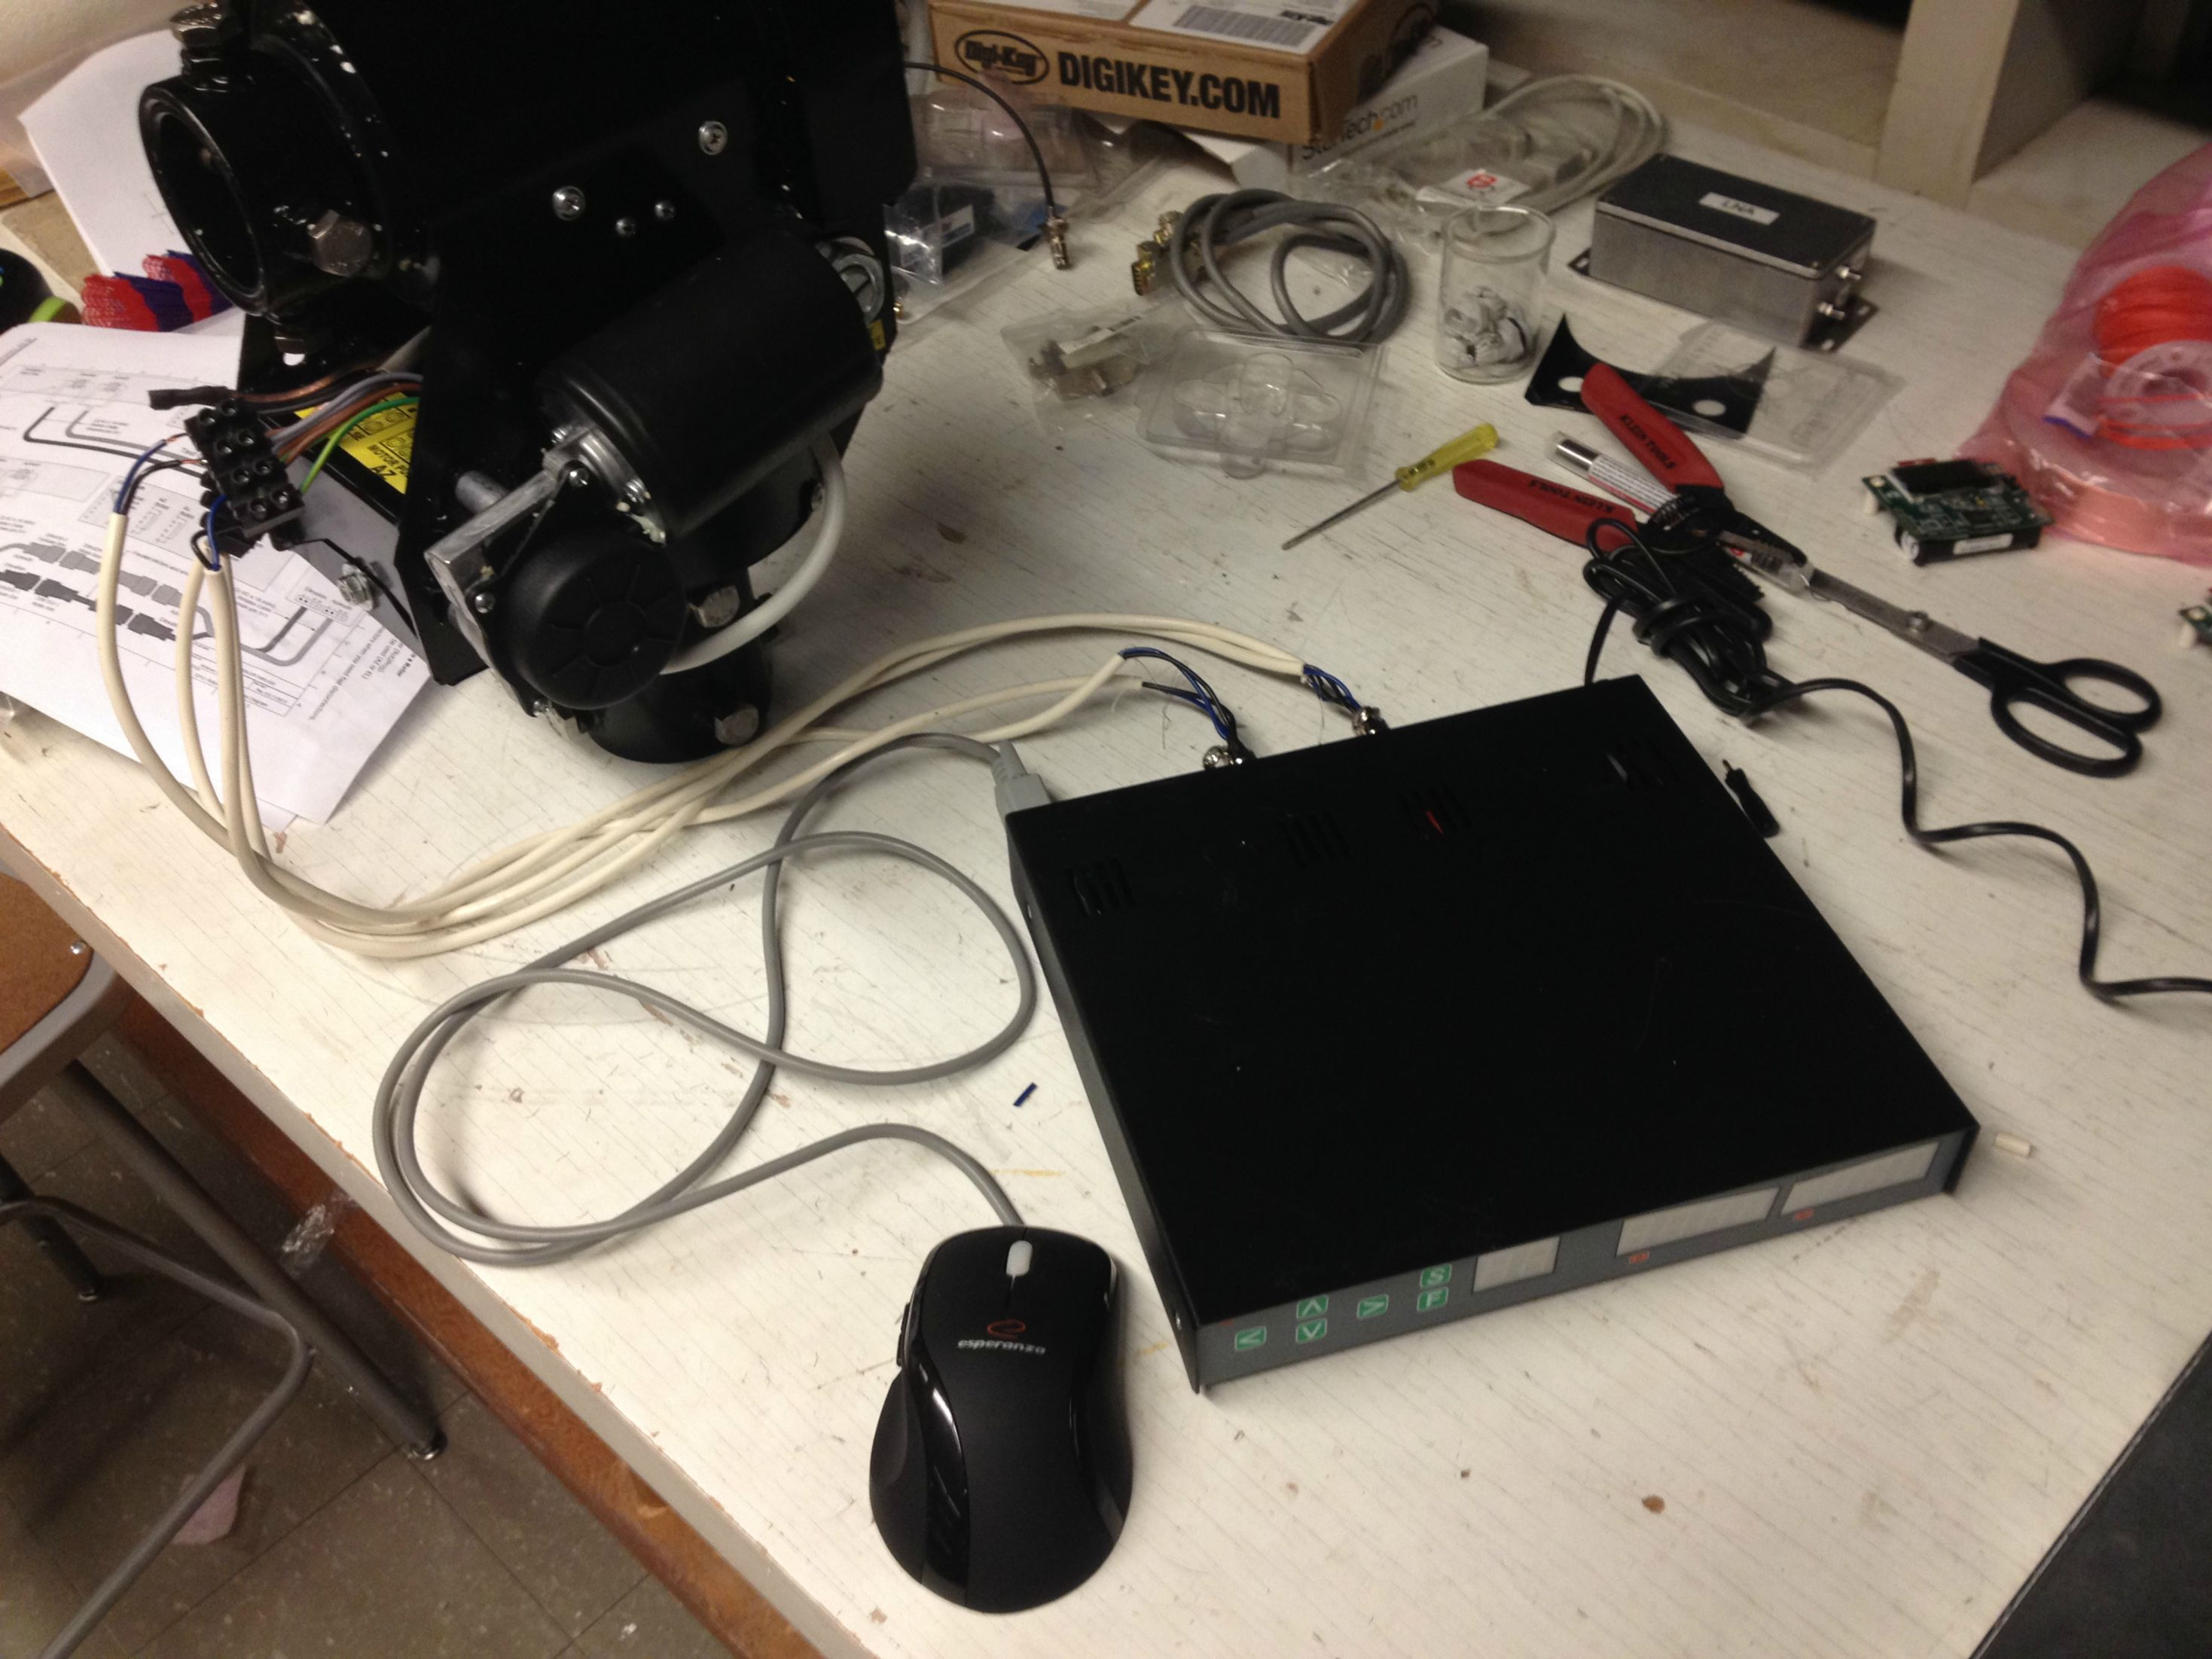
\includegraphics[scale=0.10]{wiring/10.jpeg}
\end{center}

Adjusting the the controller to be in 'A' (automatic mode), we were able to control the rotor with the mouse.








\subsection{Controller Settings}

Full documentation can be found: \\ ( http://www.spid.alpha.pl/download/AlfaSpid\_Rotator\_RAS\_EN.doc ).\\ Much of this documentation was pulled directly from the source linked above.

\subsubsection{RAS SPID rot2 Settings}

In our setup, we are using the RAS SPID rot2 Rotator. We want to have our settings such that PS (program simulation) is configured to SP. If the mode is not SP, the controller will not work. With the rotor we are using (1 degree per pulse accuracy), we also want our rotor transmission, P, to be set to 1.0. To have the computer software or mouse control the rotor, the mode will need to be set to A (automatic). For more detailed information, see the "Controller Setup" section, below.

\subsubsection{Controller Reset}

Since there are no mechanical limits in the rotor, it may be installed with the antenna pointing in any direction. There is no reason to locate “TRUE NORTH” until you are ready to calibrate the control box. Use the controller to position the antenna to physically point north, then reset the controller as follows:
\begin{itemize}
\item Turn the unit OFF.
\item While holding the F button down, turn control unit back on.
\item The display should then read 0.0 0.0
\end{itemize}

This feature can be used if, for any reason, the direction of the antenna becomes incorrect. This may be caused by antenna to mast slippage or incorrect initial alignment.
\\ \\
\textbf{Important Note:}
\\ \\
The SPID rotator is now set at the counter-clockwise end of its normal rotation range. Normal rotation range is in a clockwise direction for 360 degrees.

From the reset position, you can rotate counter-clockwise an additional 180 degrees in over-travel, as well 360 degrees clockwise, plus an additional 180 degrees into clockwise over-travel.

Counter-clockwise over-travel is indicated by a steady dot above the over-travel icon [$<$-$>$]. [$<$-$>$] Rotation past 359 degrees into the clockwise over-travel is indicated by a blinking dot above the over-travel icon.[$<$-$>$]
\\ \\
\textbf{Technical Note:}
\\ \\
You will need to leave sufficient coax length to accommodate the additional 180 degrees of over-travel on each end of normal rotation. Failure to do so can cause damage to your coax and/or antennas.

\subsubsection{Controller Operation}

There are multiple modes of operation for the SPID controller. The two main modes, F and S are described below, along with all of their sub-modes.

\subsubsection{F - Function Mode}

The F button steps through the function menus. The leftmost character on the display indicates the function mode you are currently in.
\\ \\
\textbf{(no letter) = Normal Operations Mode}
\\ \\
In Normal Operations Mode, the up, down, left, right buttons cause rotation as long as the buttons are pressed. Pressing S while in normal operations mode will take you to setup mode.
\\ \\
\textbf{H = Half-Auto Mode}
\\ \\
In Half Auto Mode, the up, down, left, right buttons can be used to pre-select the desired beam heading. The heading displayed on the controller will rapidly change in the direction of desired rotation. Once the desired beam heading is shown on the display, release the key. Approximately $\frac{1}{2}$ of a second after no key presses have been detected, the display will revert back to the actual beam heading, and rotation towards the desired heading will take place. Pressing any key while in transit to the desired heading will cancel the action.
\\ \\
\textbf{A = Auto Mode}
\\ \\
In Auto Mode, the controller will respond to commands from control software running on an attached computer. The up, down, left, right buttons can still be used, but pressing of any of them will cause canceling the data from software.

\subsubsection{S - Setup Mode}

The S button steps through the setup menu.
\\ \\
\textbf{P = Rotor Transmission}
\\ \\
This value defines the accuracy of rotator operation. 1.0 means operating with up to 1 degree per pulse from rotator accuracy.
\\ \\
\textbf{PS = Program Simulation}
\\ \\
Program Simulation allows the user to set the serial communication protocol used by the rotator. When set to emulate another brand of rotator, the Spid will respond to commands, and send responses back to the computer as if it were the rotator brand selected. If your favorite software supports a rotator, chances are, the Spid will be able to interface to your software. There are 2 modes available:	
\begin{itemize}
\item PS SP = SPID
\item PS 4A = Yaesu (GS232 protocol)
\end{itemize}
(RS232: 600N1, 8 bits)
\\ \\
(data rate bound 600, 1 STOP bit, no even parity bit)
\\ \\
Operating mode can be changed using left, right.
\\ \\
\textbf{PH = Programmable High Limit}
\\ \\
The Programmable High Limit is a user adjustable clockwise travel limit value. By reducing this value, the maximum clockwise rotation travel can be restricted. Use the buttons:
\begin{itemize}
\item \emph{left} and \emph{right} to adjust the azimuth value,
\item \emph{up} and \emph{down} to adjust the elevation value.
\end{itemize}

\textbf{PL = Programmable Low Limit}
\\
The Programmable Low Limit is a user adjustable counter-clockwise travel limit value. By increasing this value, the minimum counter-clockwise rotation travel can be restricted. Use the buttons:
\begin{itemize}
\item \emph{left} and \emph{right} to adjust the azimuth value,
\item \emph{up} and \emph{down} to adjust the elevation value.
\end{itemize}
\textbf{PP = Heading Adjust}
\\ \\
This setting can be used to make minor heading adjustments without causing the rotator to turn. If you notice that the heading displayed on the controller to a known signal source is out by a few degrees, you can change the heading displayed on the LED readout to match the known heading, rather than having to turn back to North and reset the controller. These settings are made by up, down, left, right buttons.






\subsection{Controller Setup}


The antenna controller will likely need a bit of setup in order to work properly with the software. To properly set up the controller, three things must be done: 

\begin{enumerate}
\item Make sure the controller has no limits set
\item Set the controller to SPID mode
\item Set the controller to Automatic mode so it is able to communicate with a computer via serial
\end{enumerate}

\subsubsection{Setting Limits}

The easiest way to be sure there are no limits set on the controller is by doing a controller reset. To do this, turn off the controller, hold down the 'F' button, and while still holding down the button turn the controller on again. When this happens the display should look like this:

\begin{center}
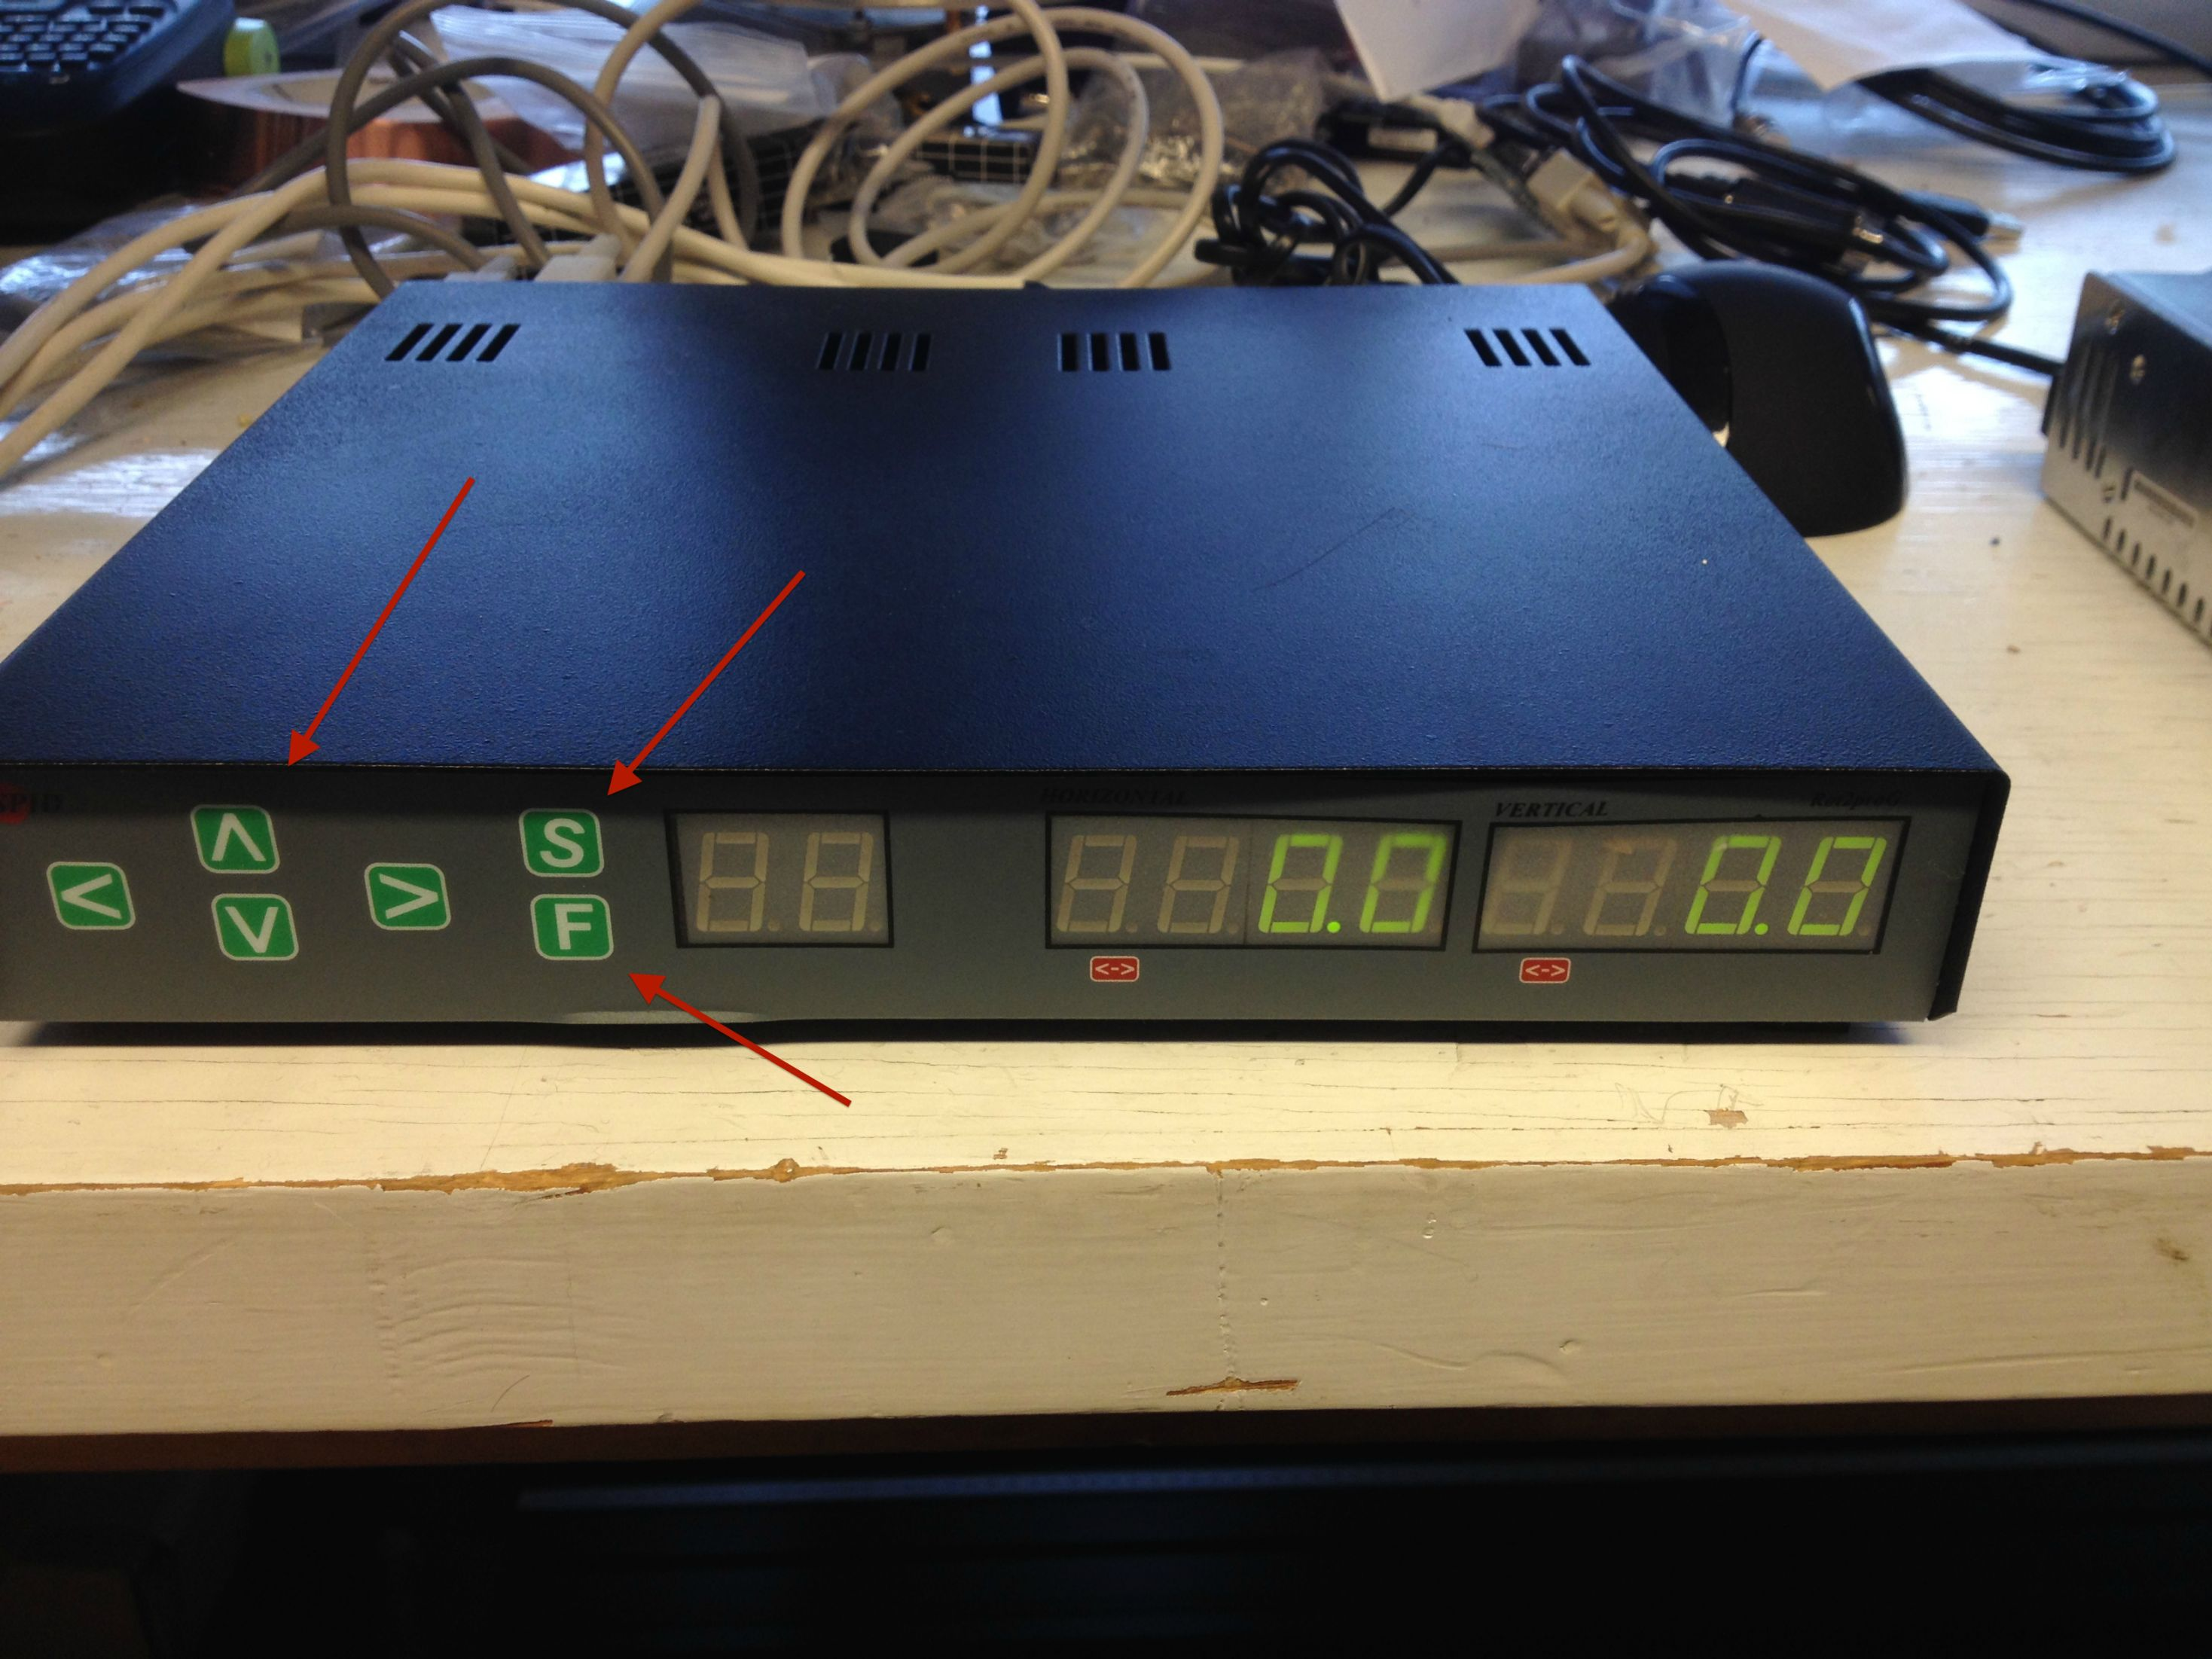
\includegraphics[scale=0.10]{controller/01.jpeg}
\end{center}

To change the remaining settings, we will use the buttons on the controller, designated by the red arrows. (F, S, \emph{left}, \emph{right}, \emph{up}, \emph{down})
\\ \\
If there are limits set, it is possible that when the software is run, a buffer overflow may occur, and that the GUI logic breaks, leading the program to be ineffective. If no radio data is being displayed on the UI and large values/NaN appear on the readout, having limits set is a potential cause.

\subsubsection{Setting to SPID}

In the controller's program simulation setting, two options are available, SPID or Yaesu. Since the controller we used is SPID, the controller should be set to SPID. To set, press the 'S' button until the readout says PS. Then, if the readout does not say PS SP, press the $<$ or $>$ arrows to change it to SP. It should look like:

\begin{center}
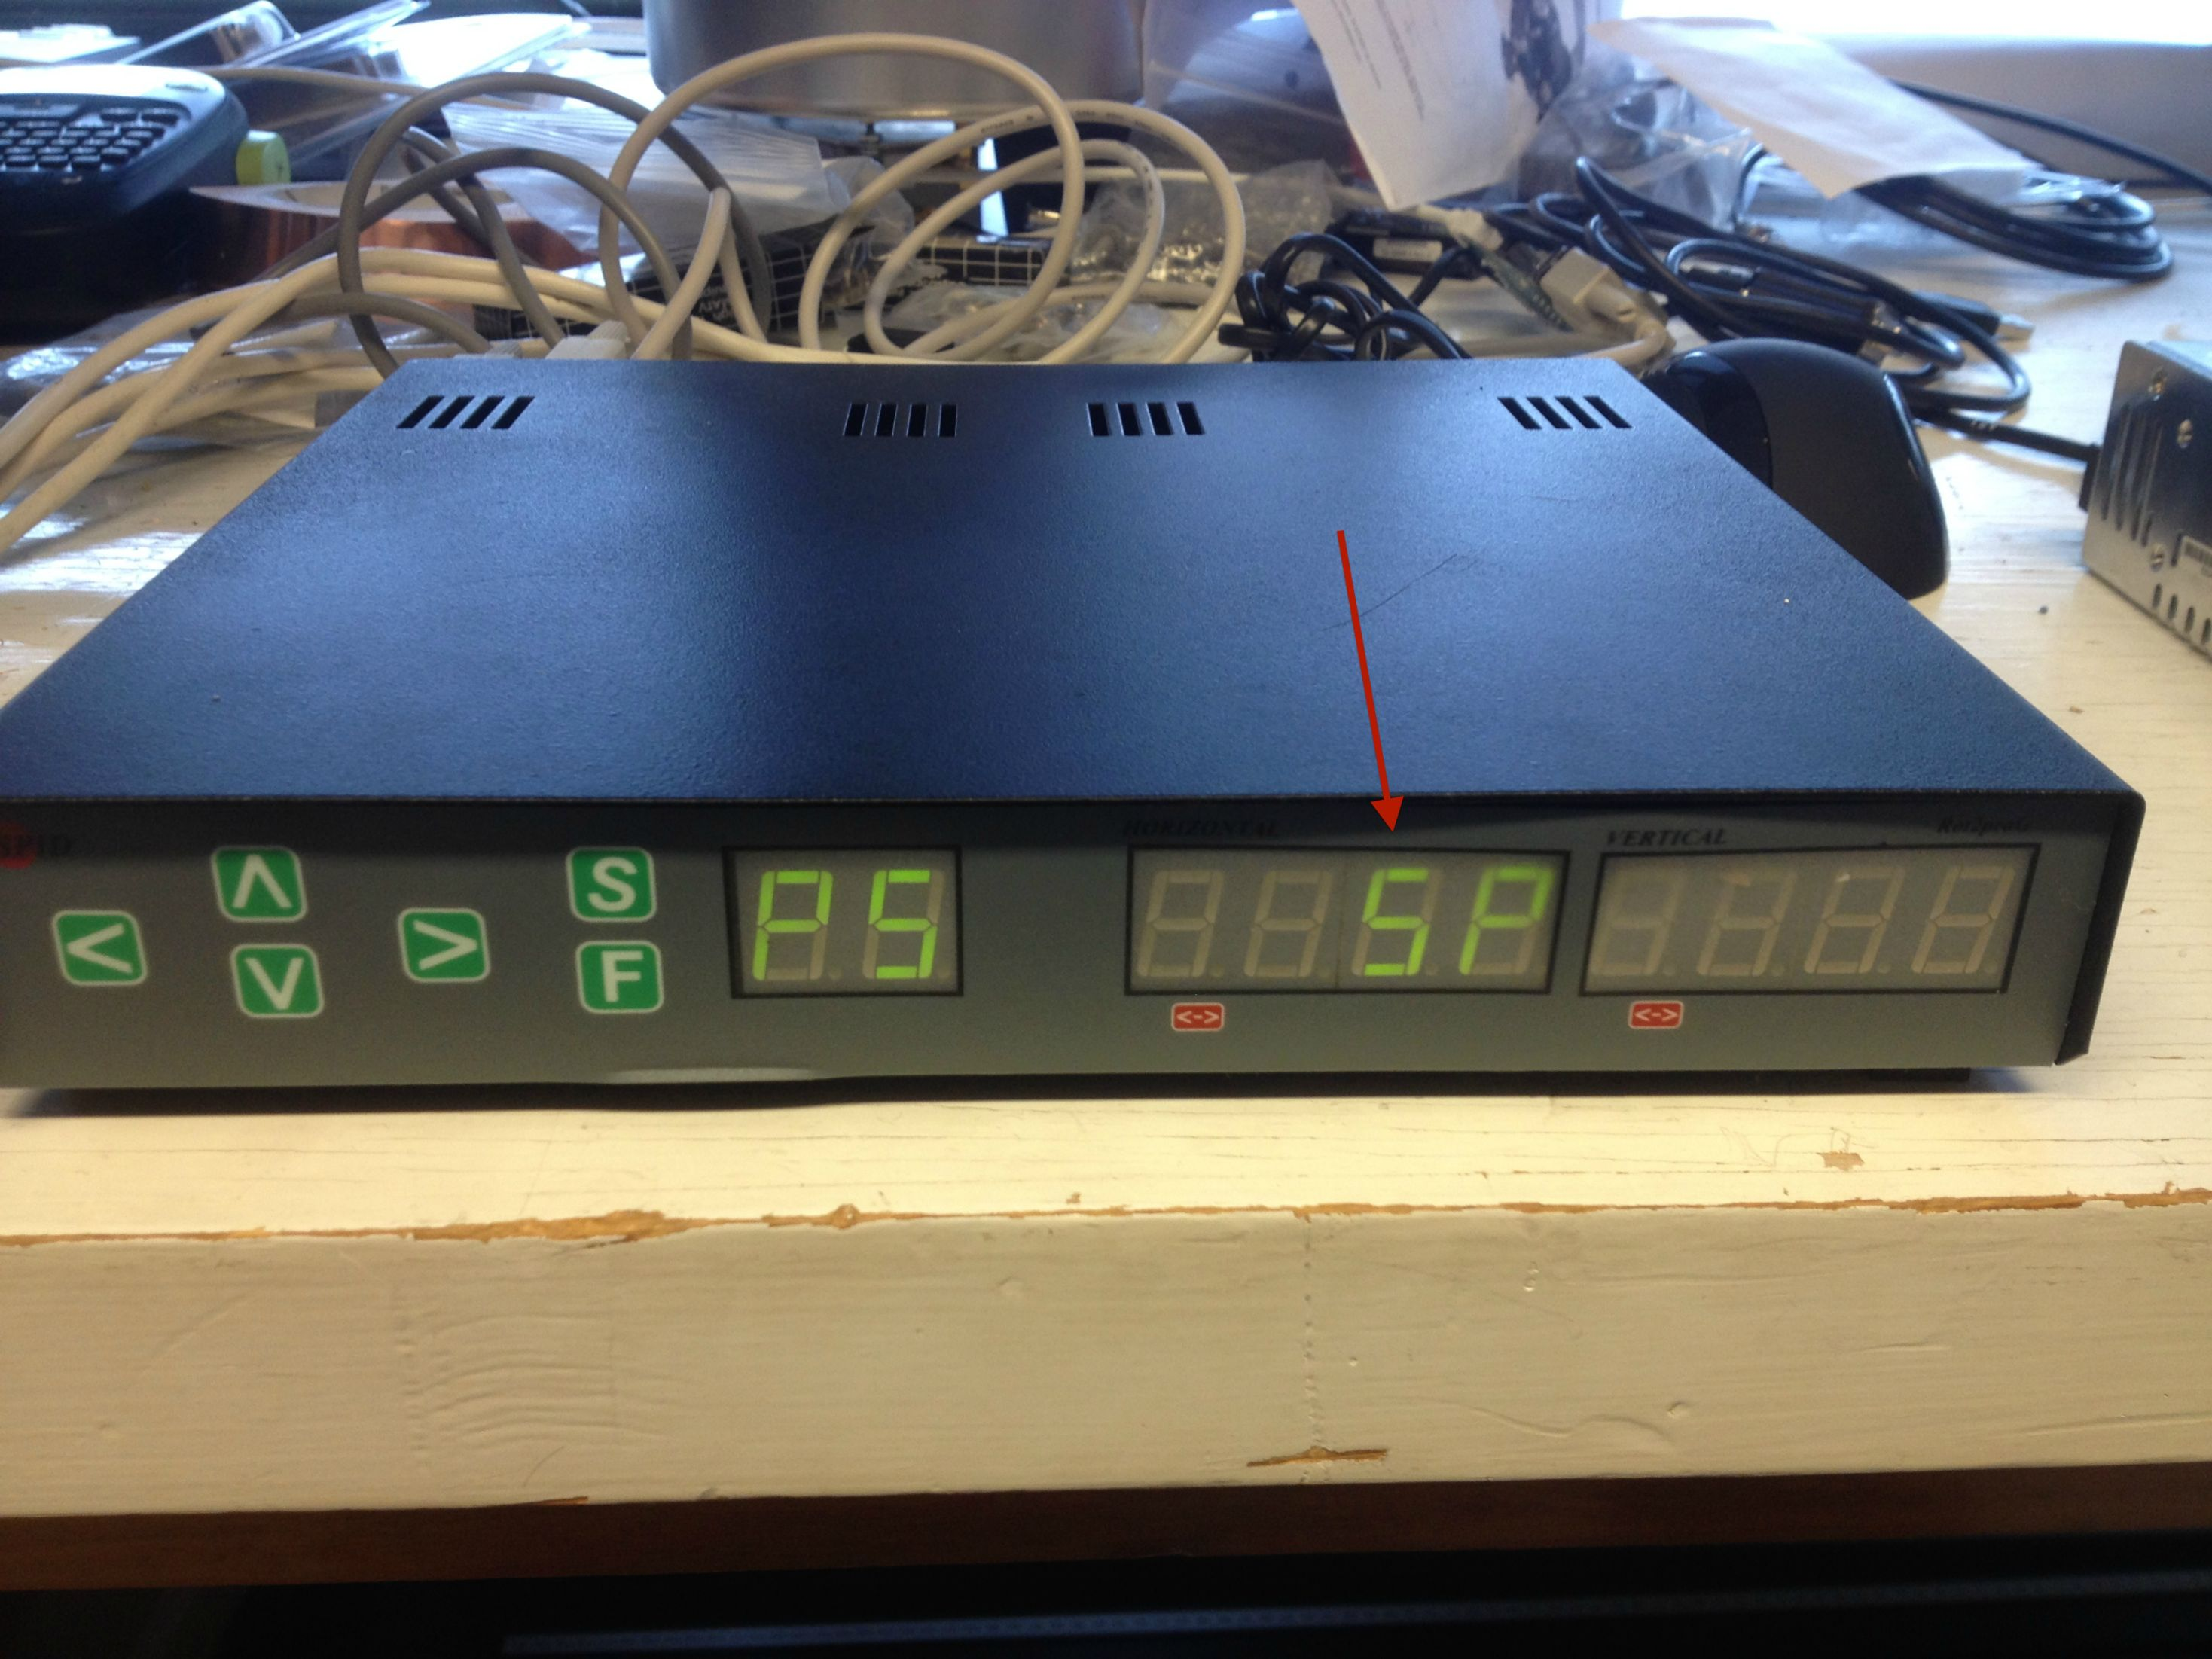
\includegraphics[scale=0.10]{controller/02.jpeg}
\end{center}

If the controller is not in SPID mode, nothing will happen and the program may hang, as it is unable to communicate with the controller.

\subsubsection{Set to Automatic}

In order for the computer to be able to communicate with the controller, it must be in automatic mode. To do this, you would press the 'F' button until an A shows up on the readout. The readout should look like:

\begin{center}
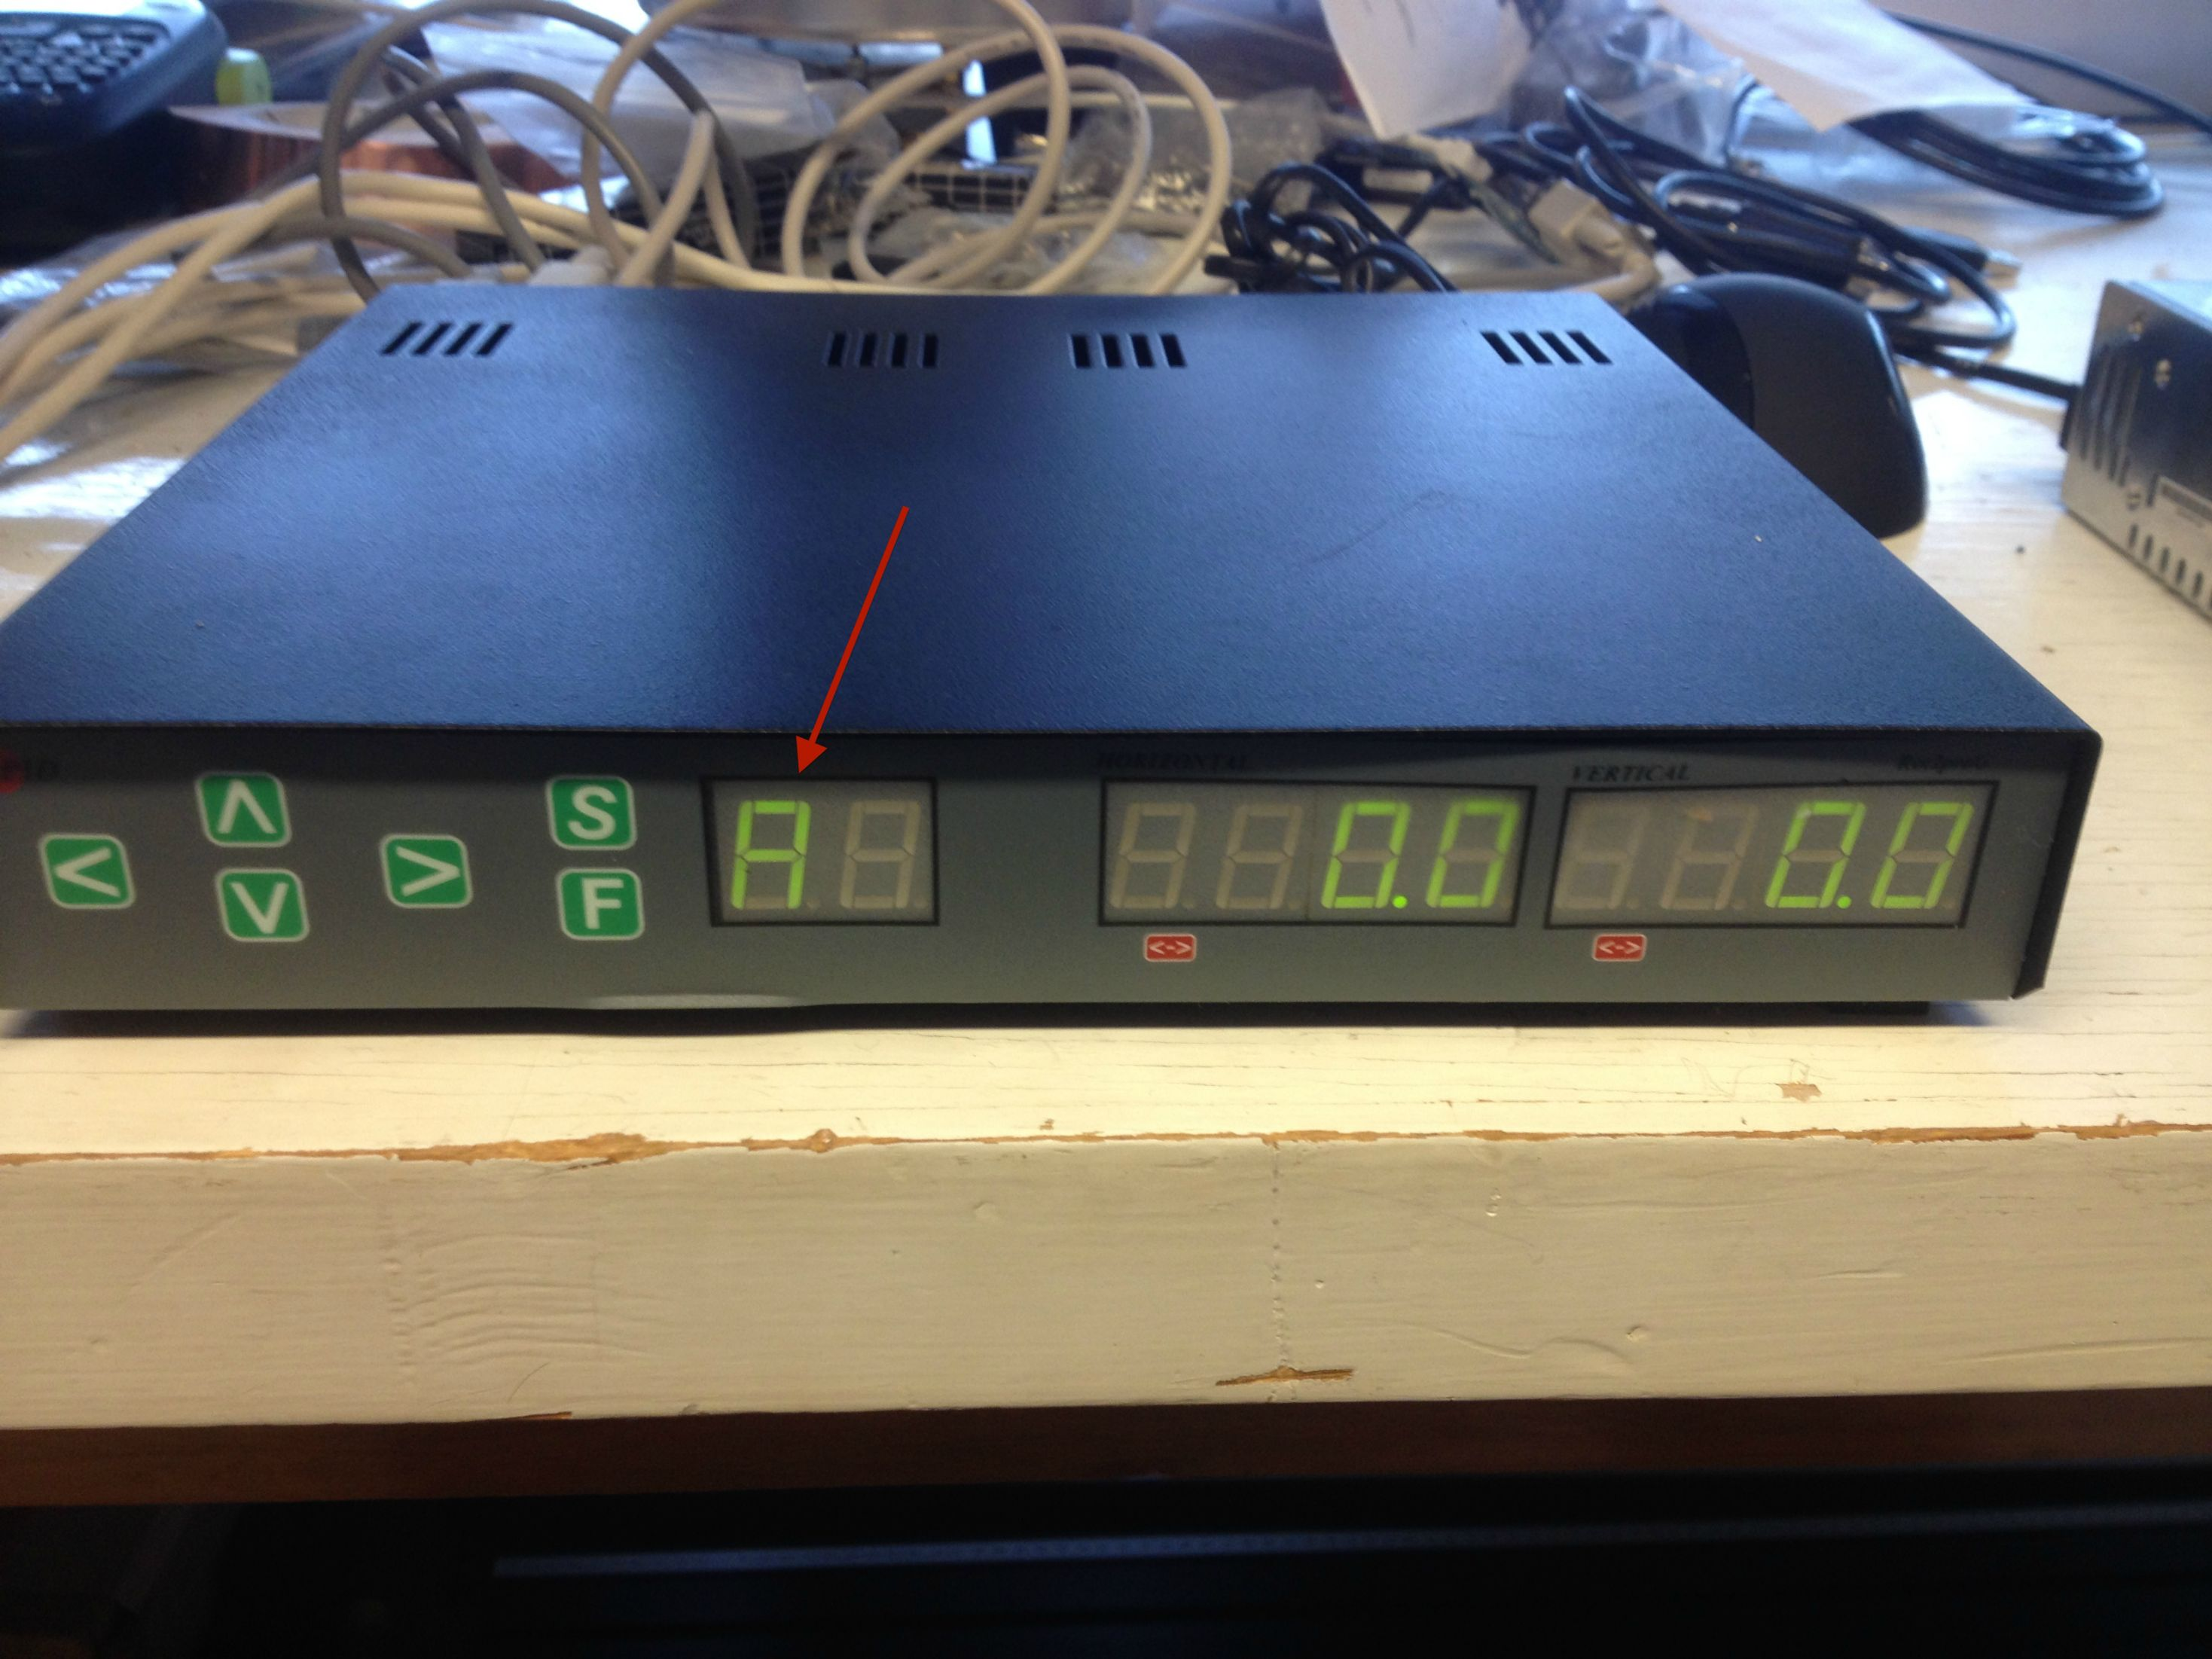
\includegraphics[scale=0.10]{controller/03.jpeg}
\end{center}

\subsubsection{Controller Wiring}

While the controller does not have many/complicated connections, and the documentation is fairly good for what connects where, below is a picture detailing our connection setup, for reference.

\begin{center}
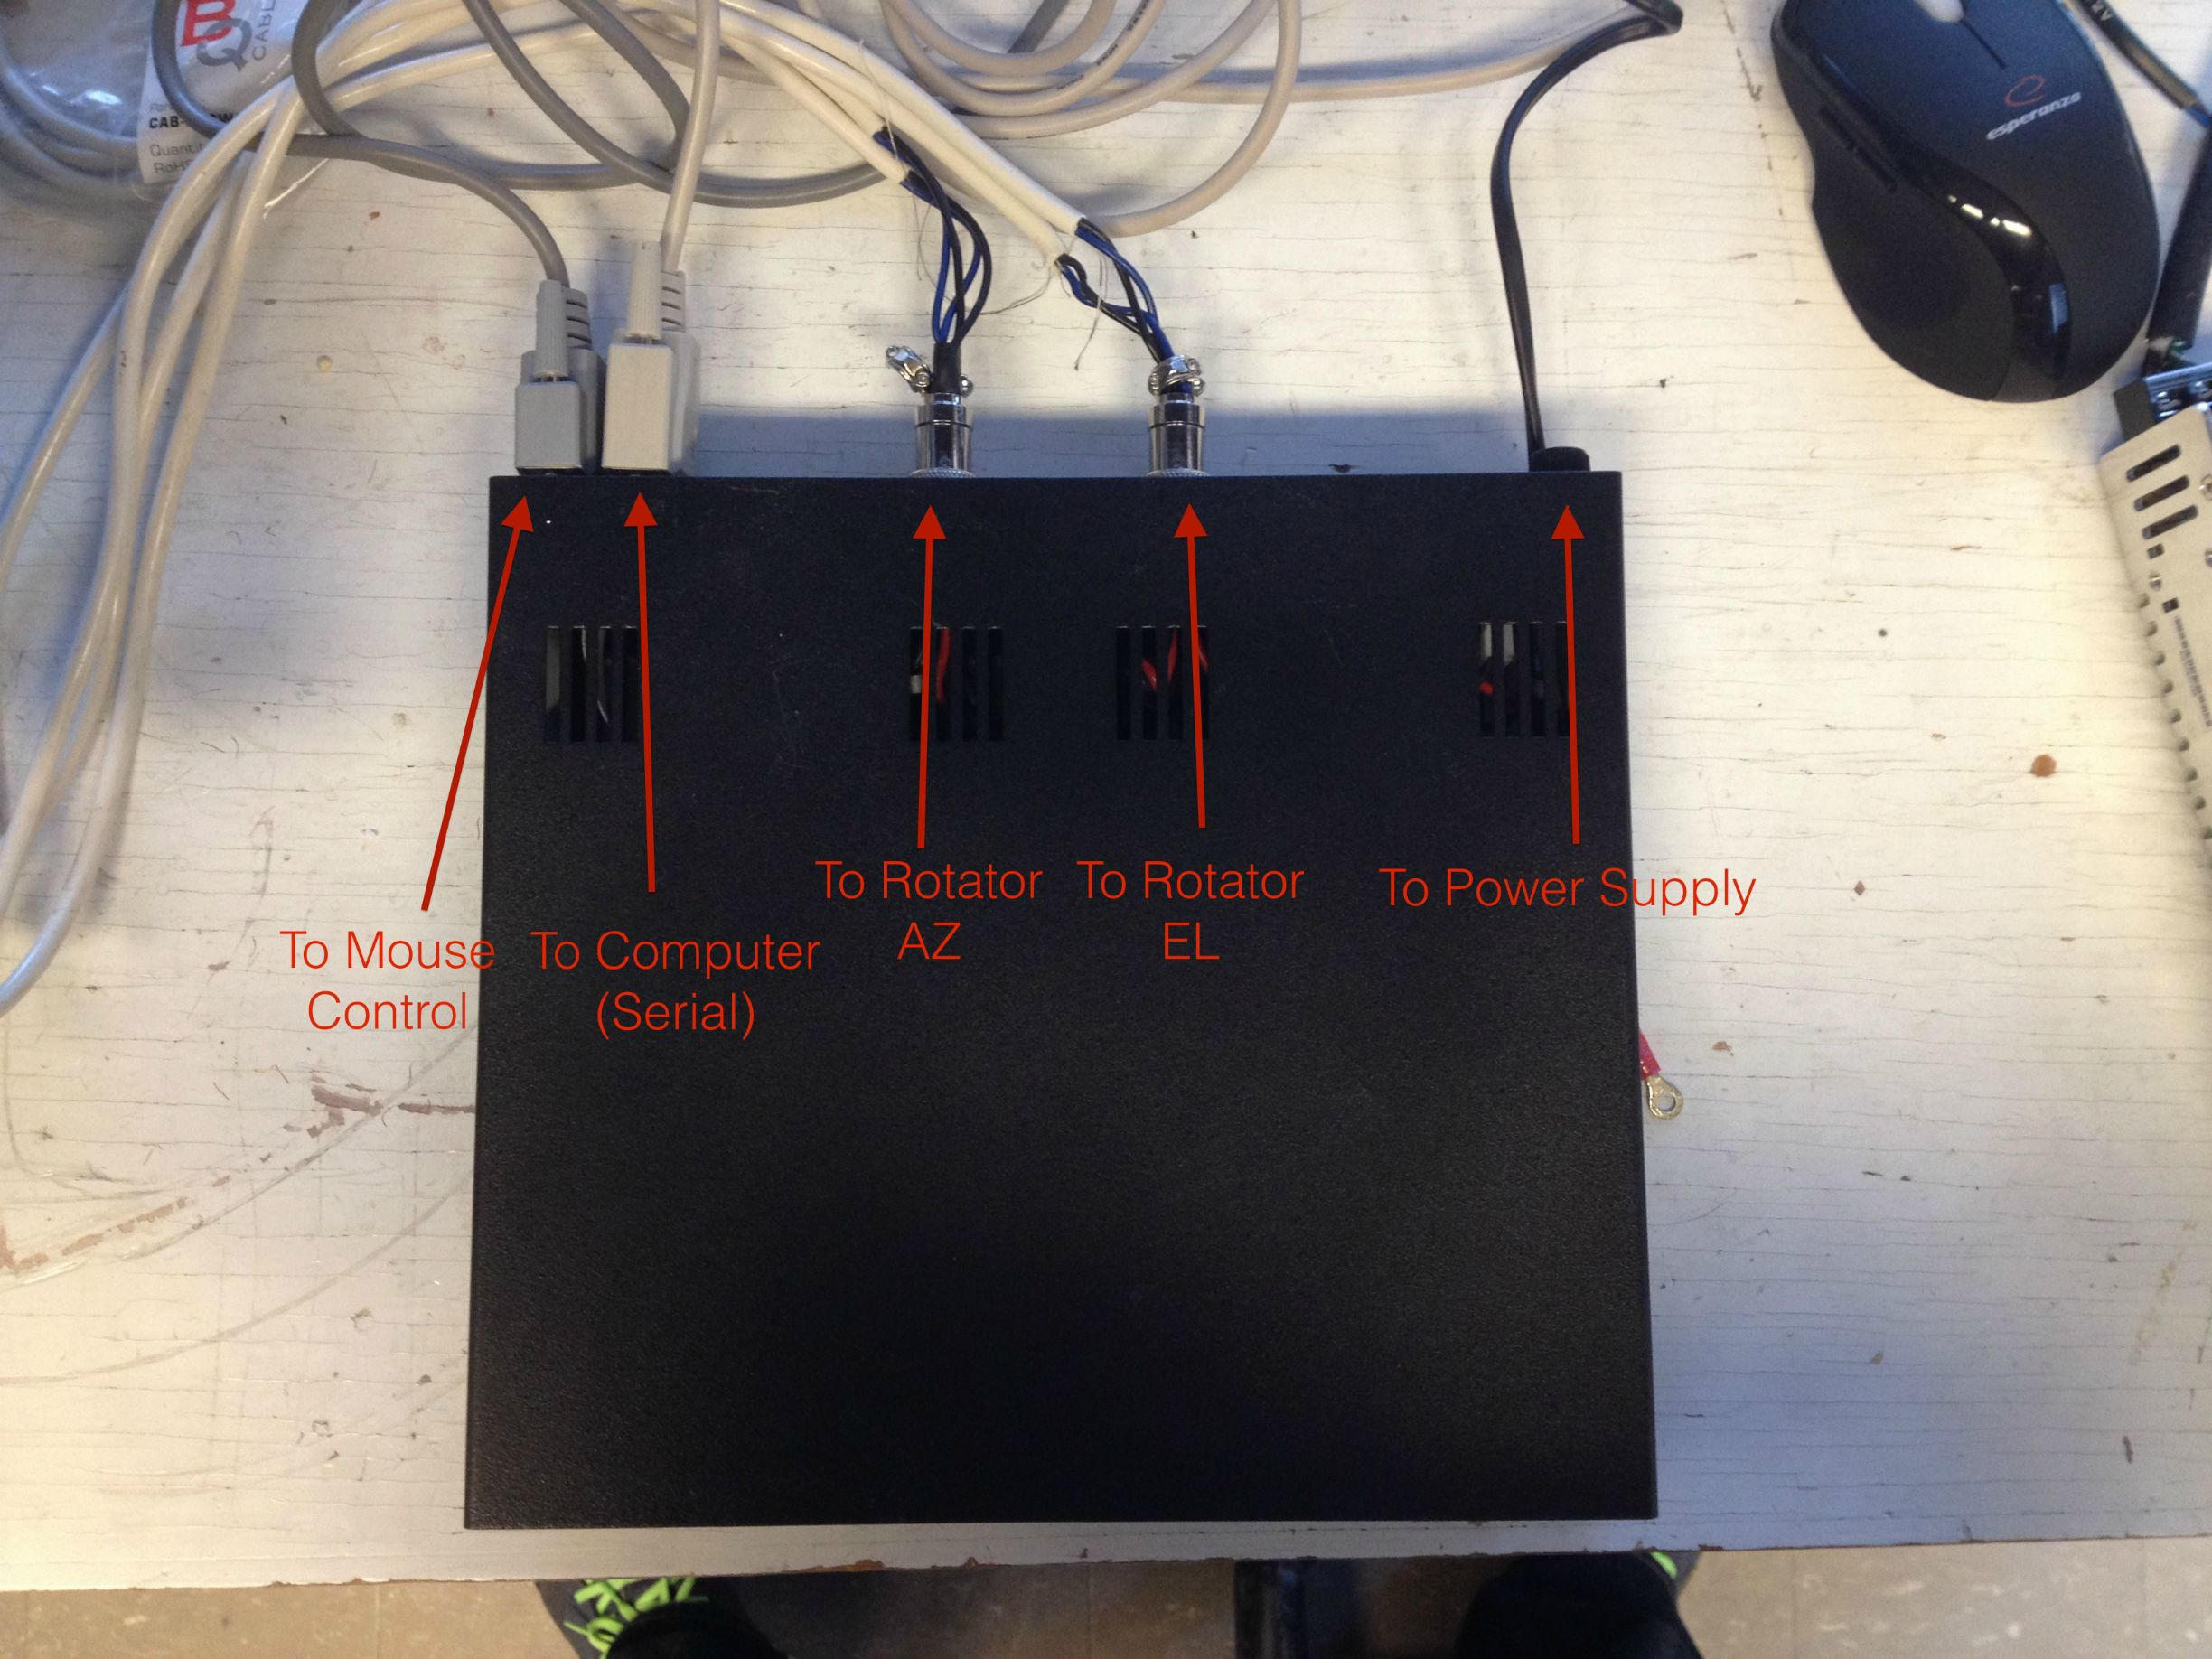
\includegraphics[scale=0.15]{controller/04.jpeg}
\end{center}


%%%%%%%%%%%%%%%%%%%%%%%%%%%%%%%%%%%%%%%%
\newpage
\section{Building Components}


\subsection{LNA}

Attached the coupler to the "In" side of Amp 1.
Then attached the bandpass filter to the "Out" side of Amp 1. 

\begin{center}
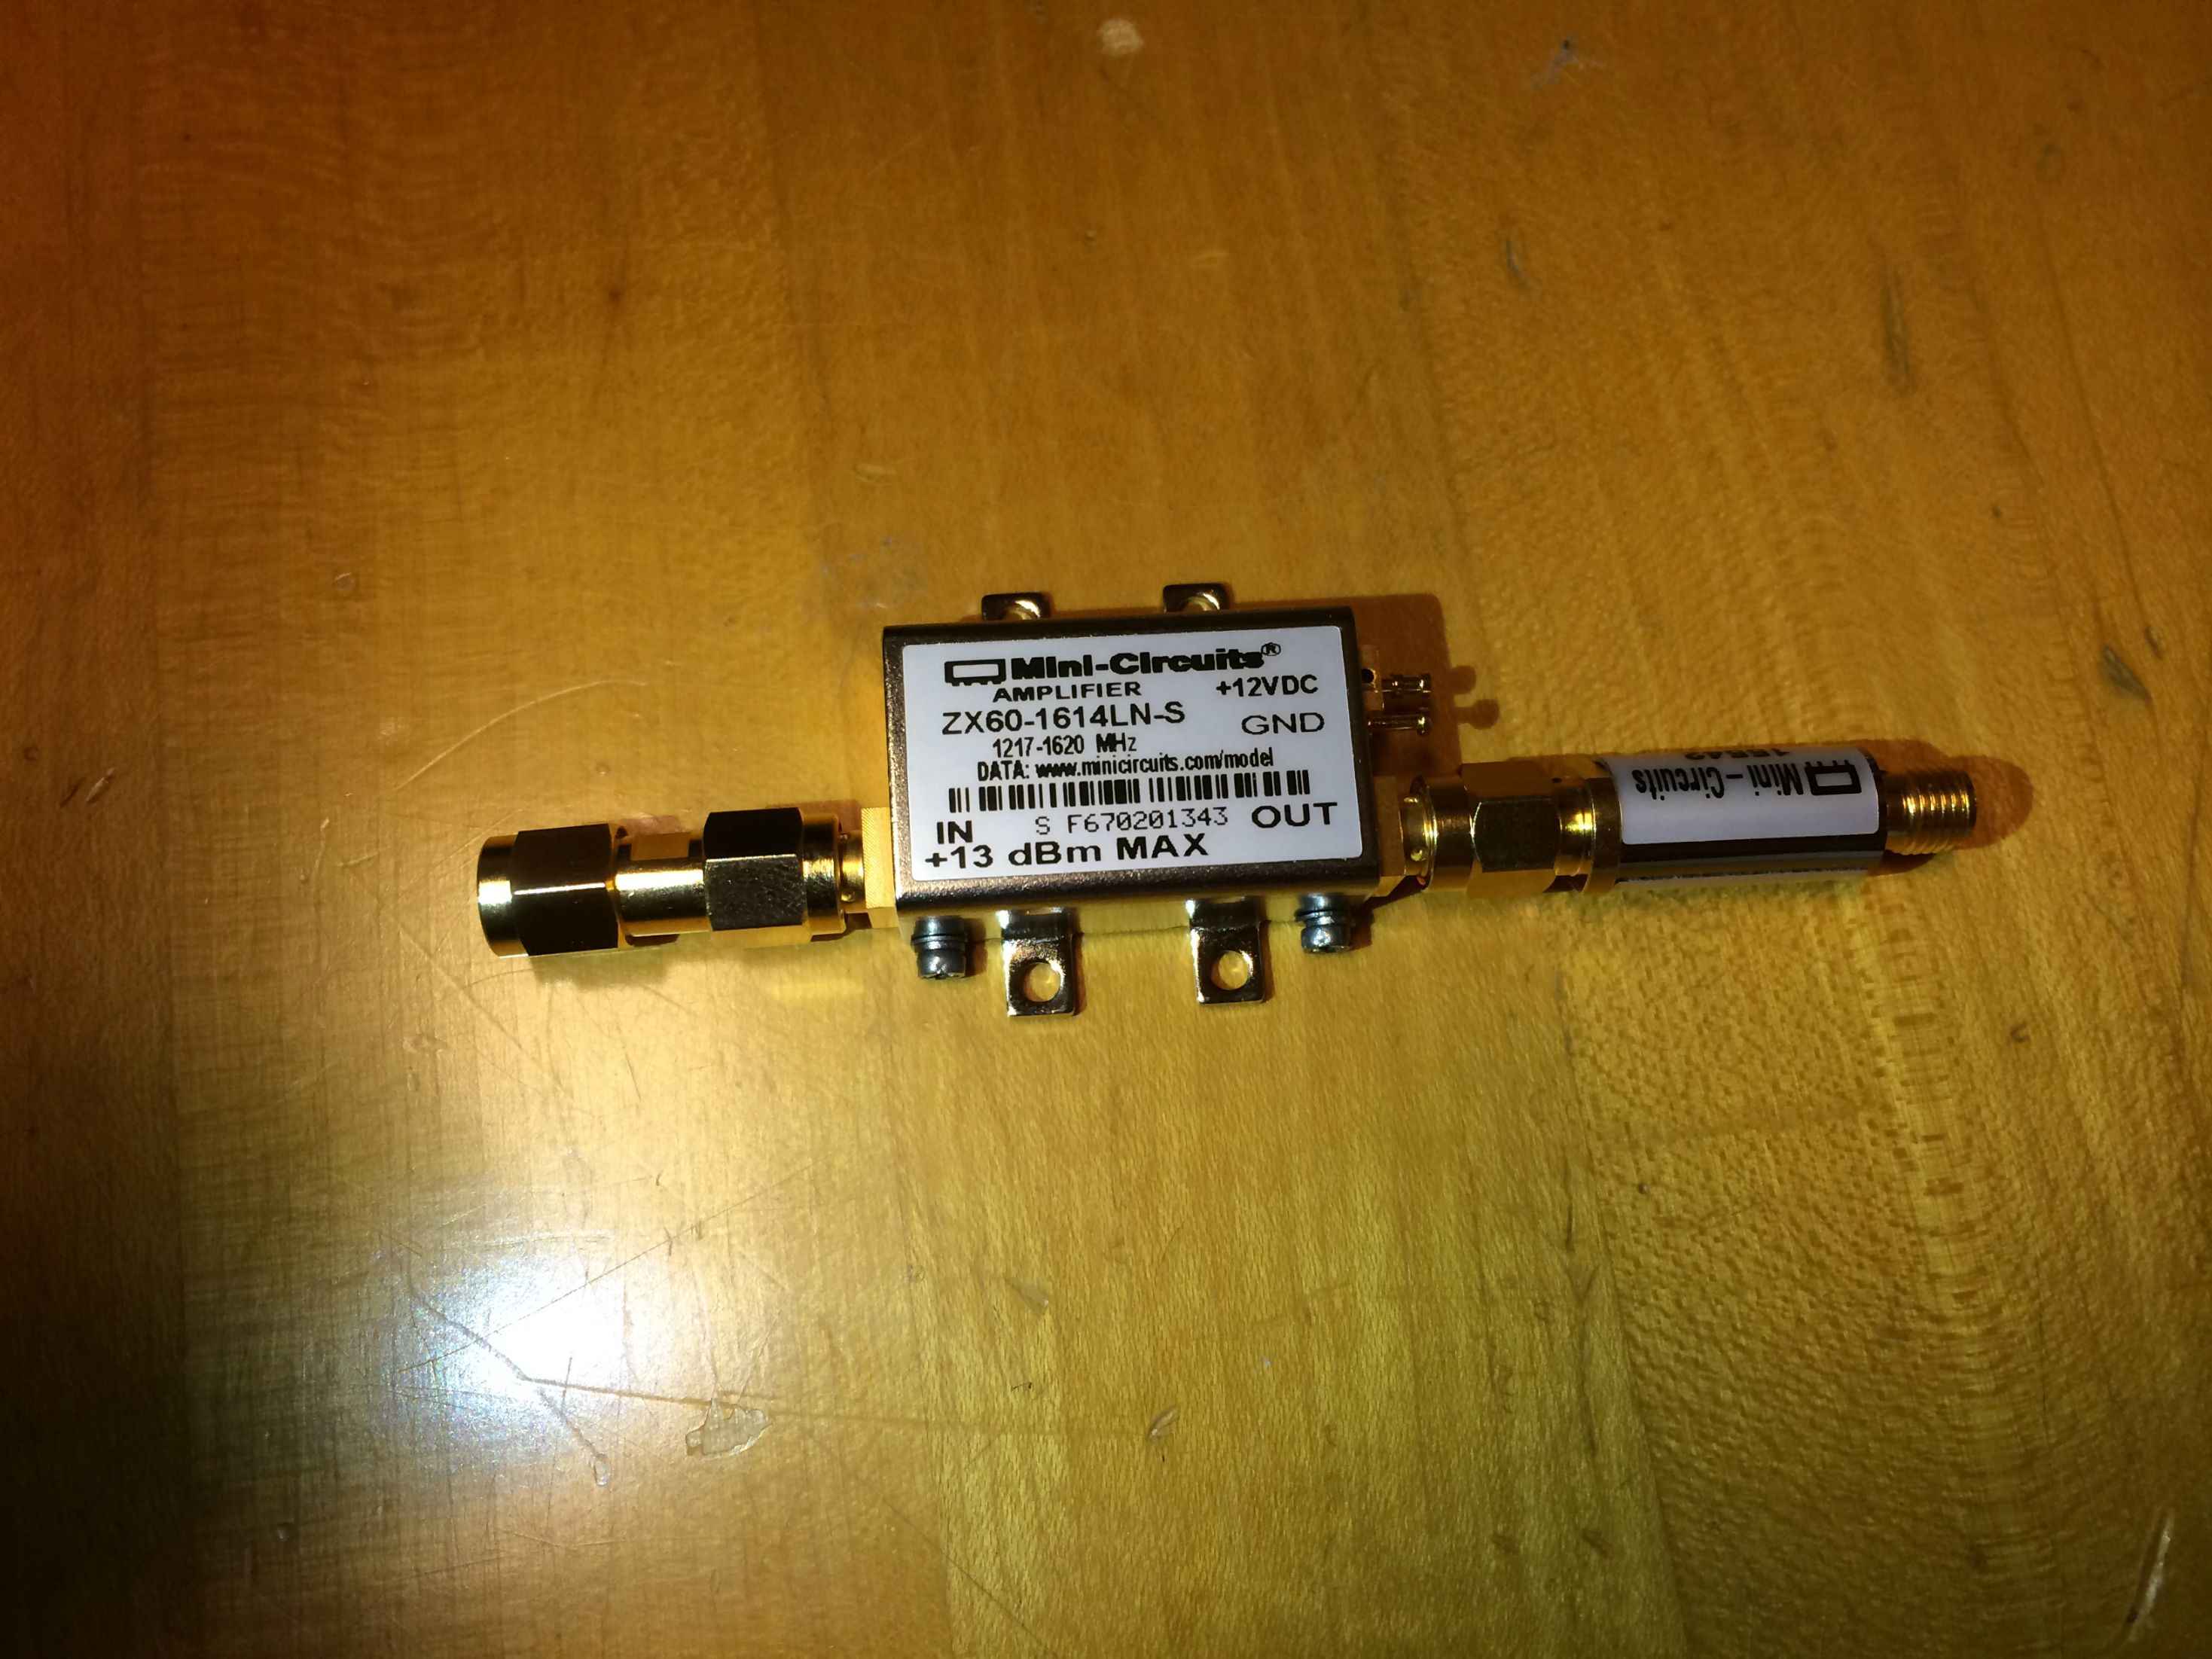
\includegraphics[scale=0.12]{lna/01.jpeg}
\end{center}

Connected one coaxial cable to bandpass. 

\begin{center}
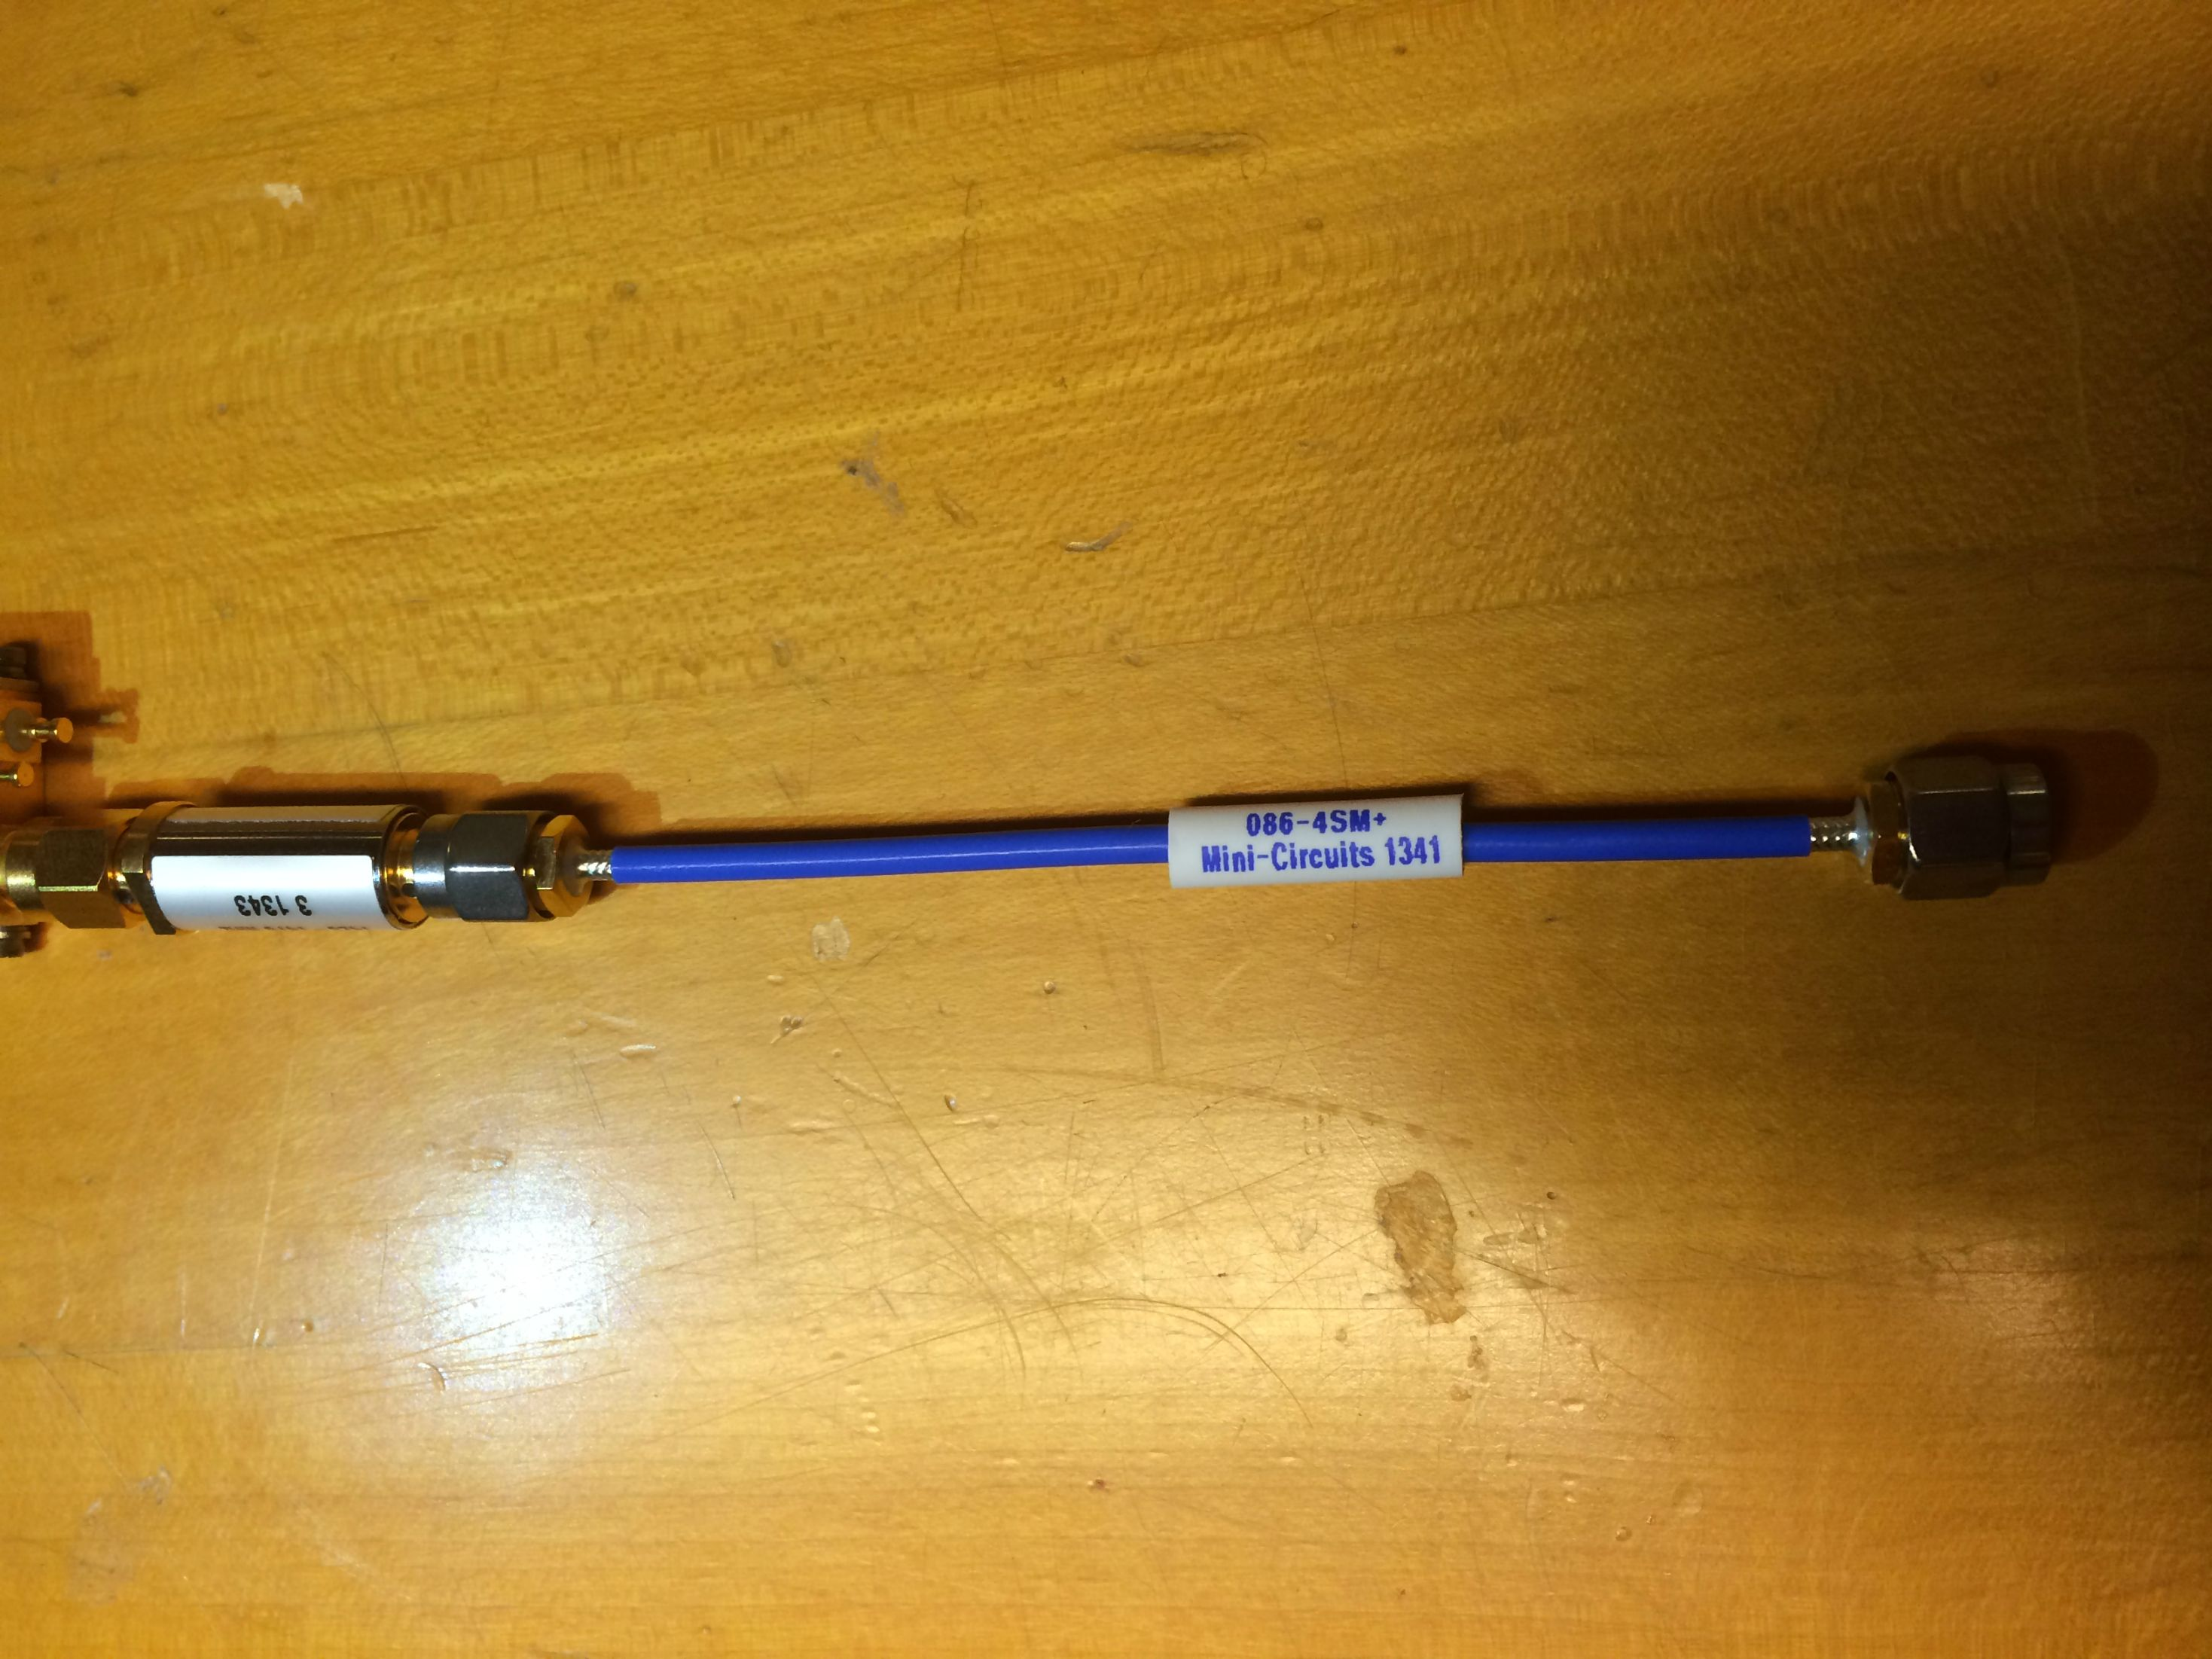
\includegraphics[scale=0.12]{lna/02.jpeg}
\end{center}

Connected opposite end of coaxial cable to "In" side of Amp 2. 

\begin{center}
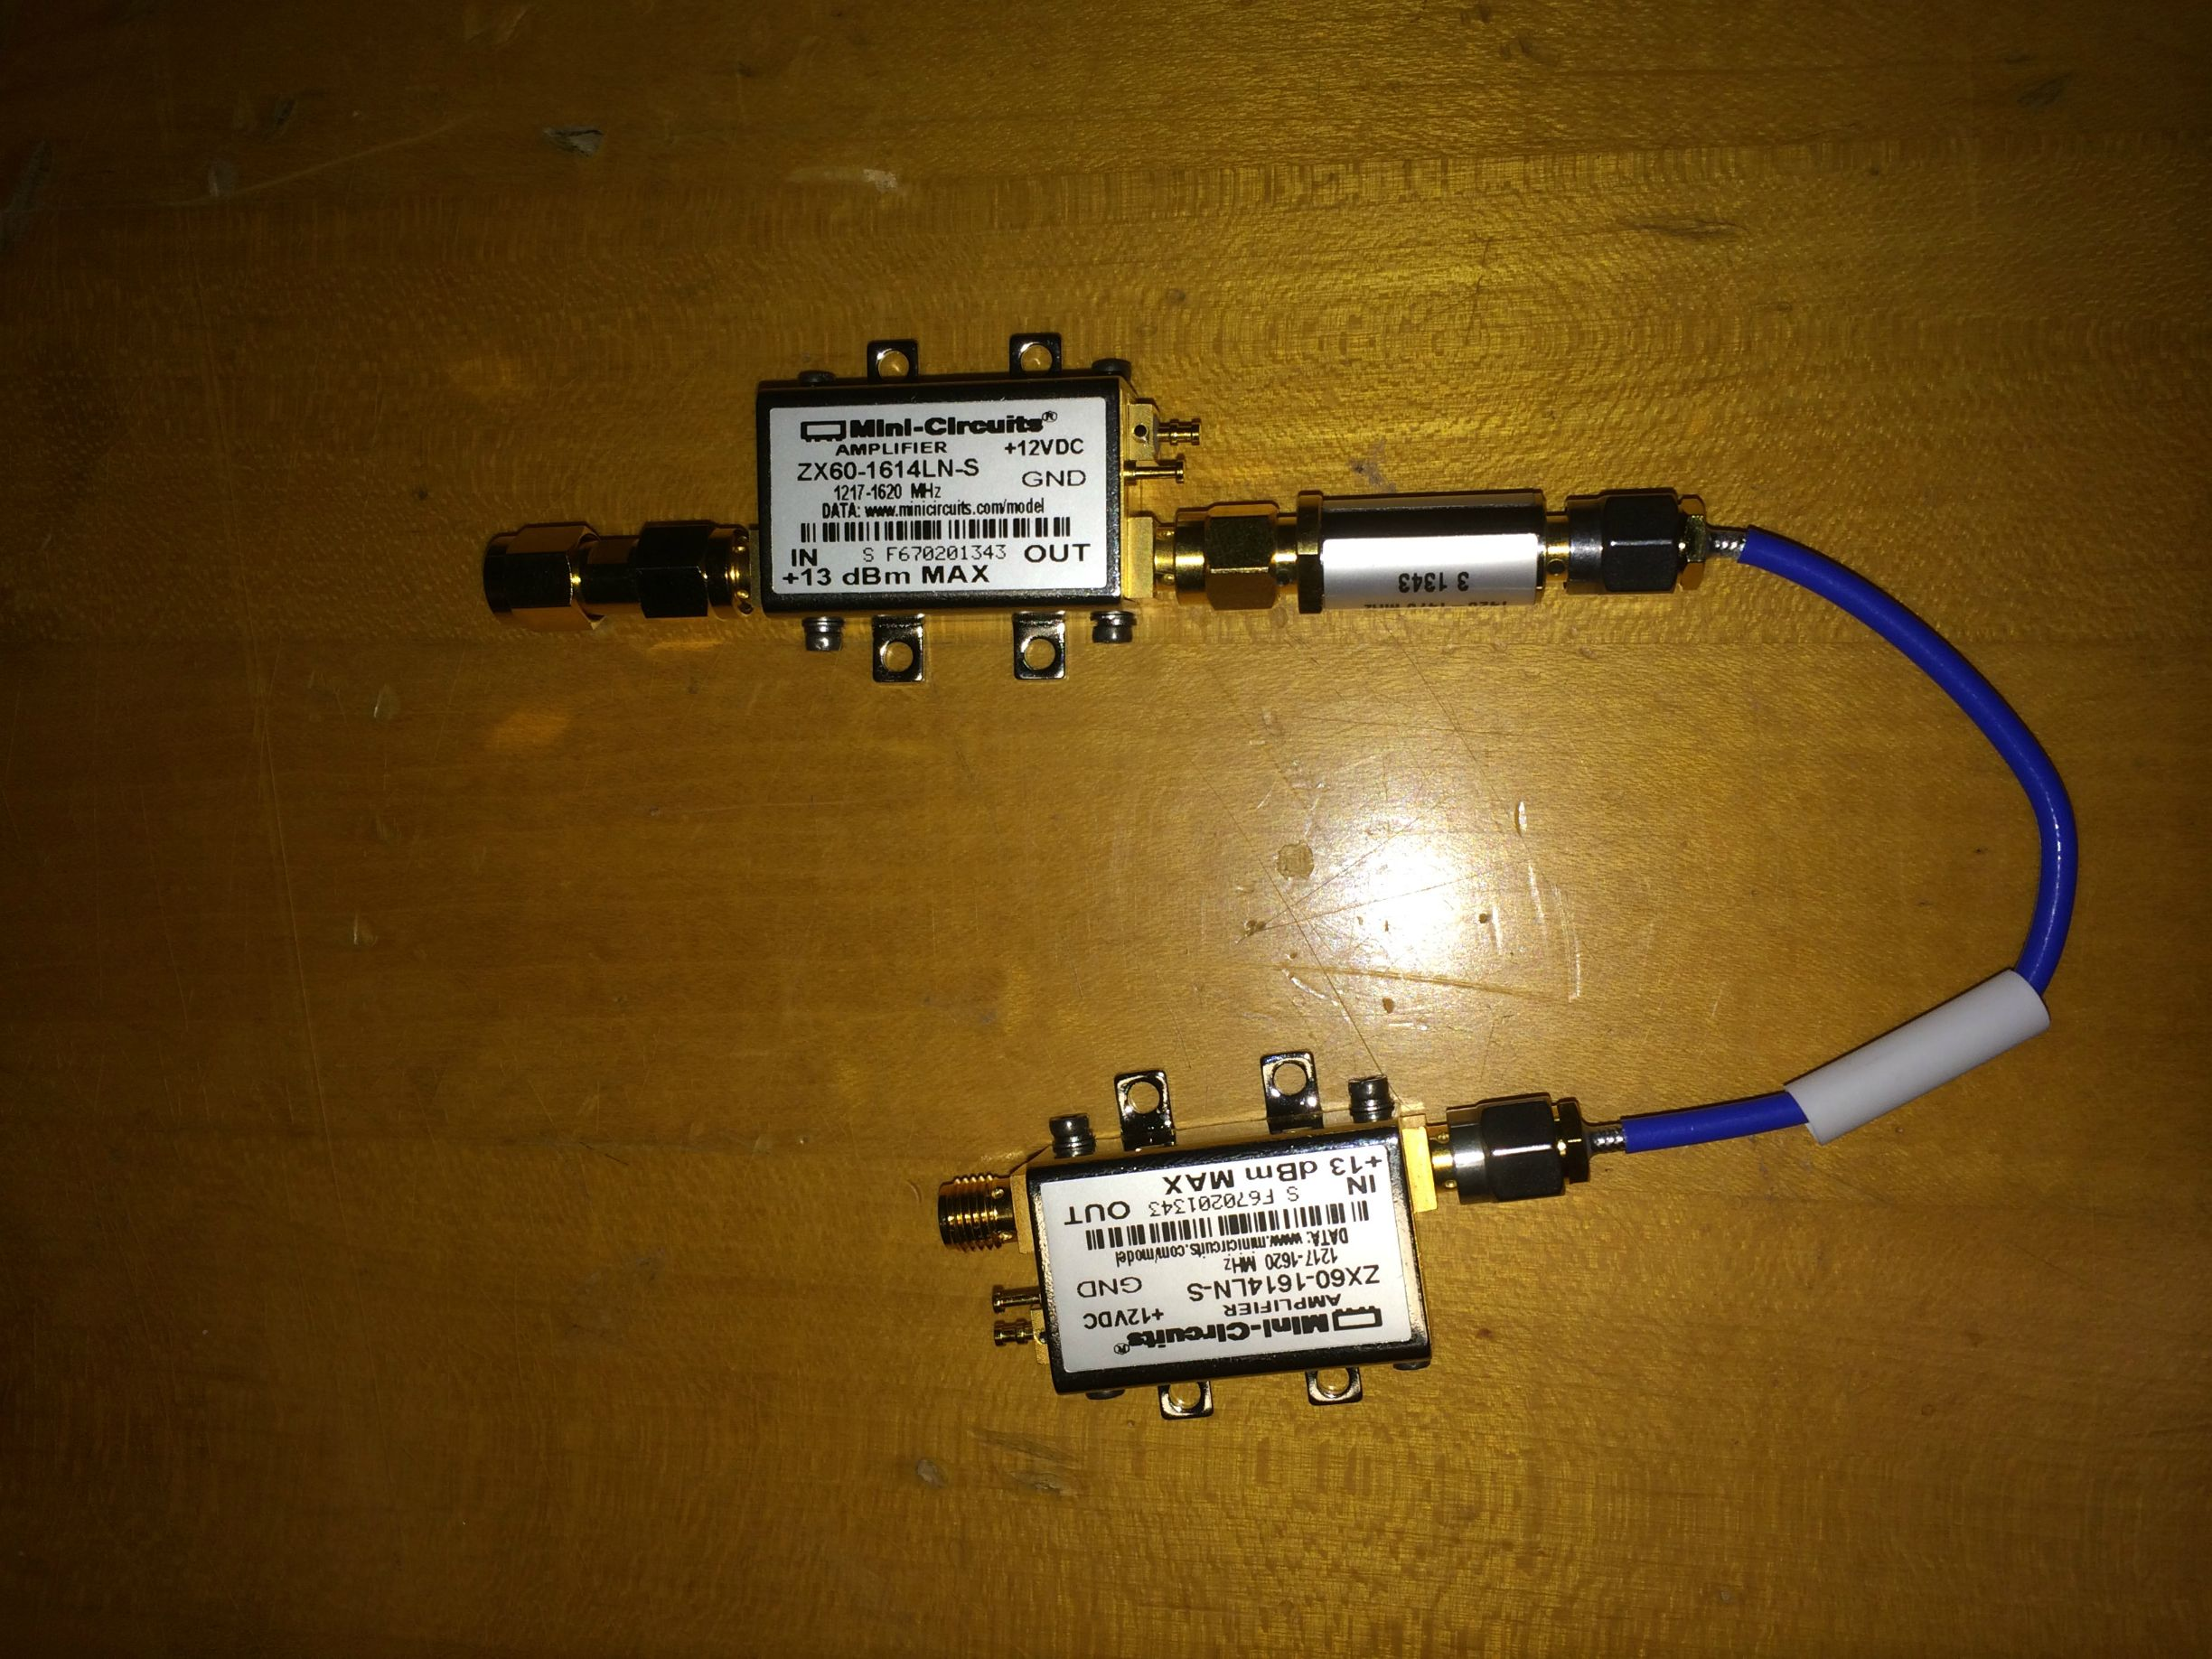
\includegraphics[scale=0.14]{lna/03.jpeg}
\end{center}

Cut two lengths of 15-20 centimeter long 22 gauge copper wire. 
Soldered one wire to both Amps.
Soldered the other wire to Amp 2. 

\begin{center}
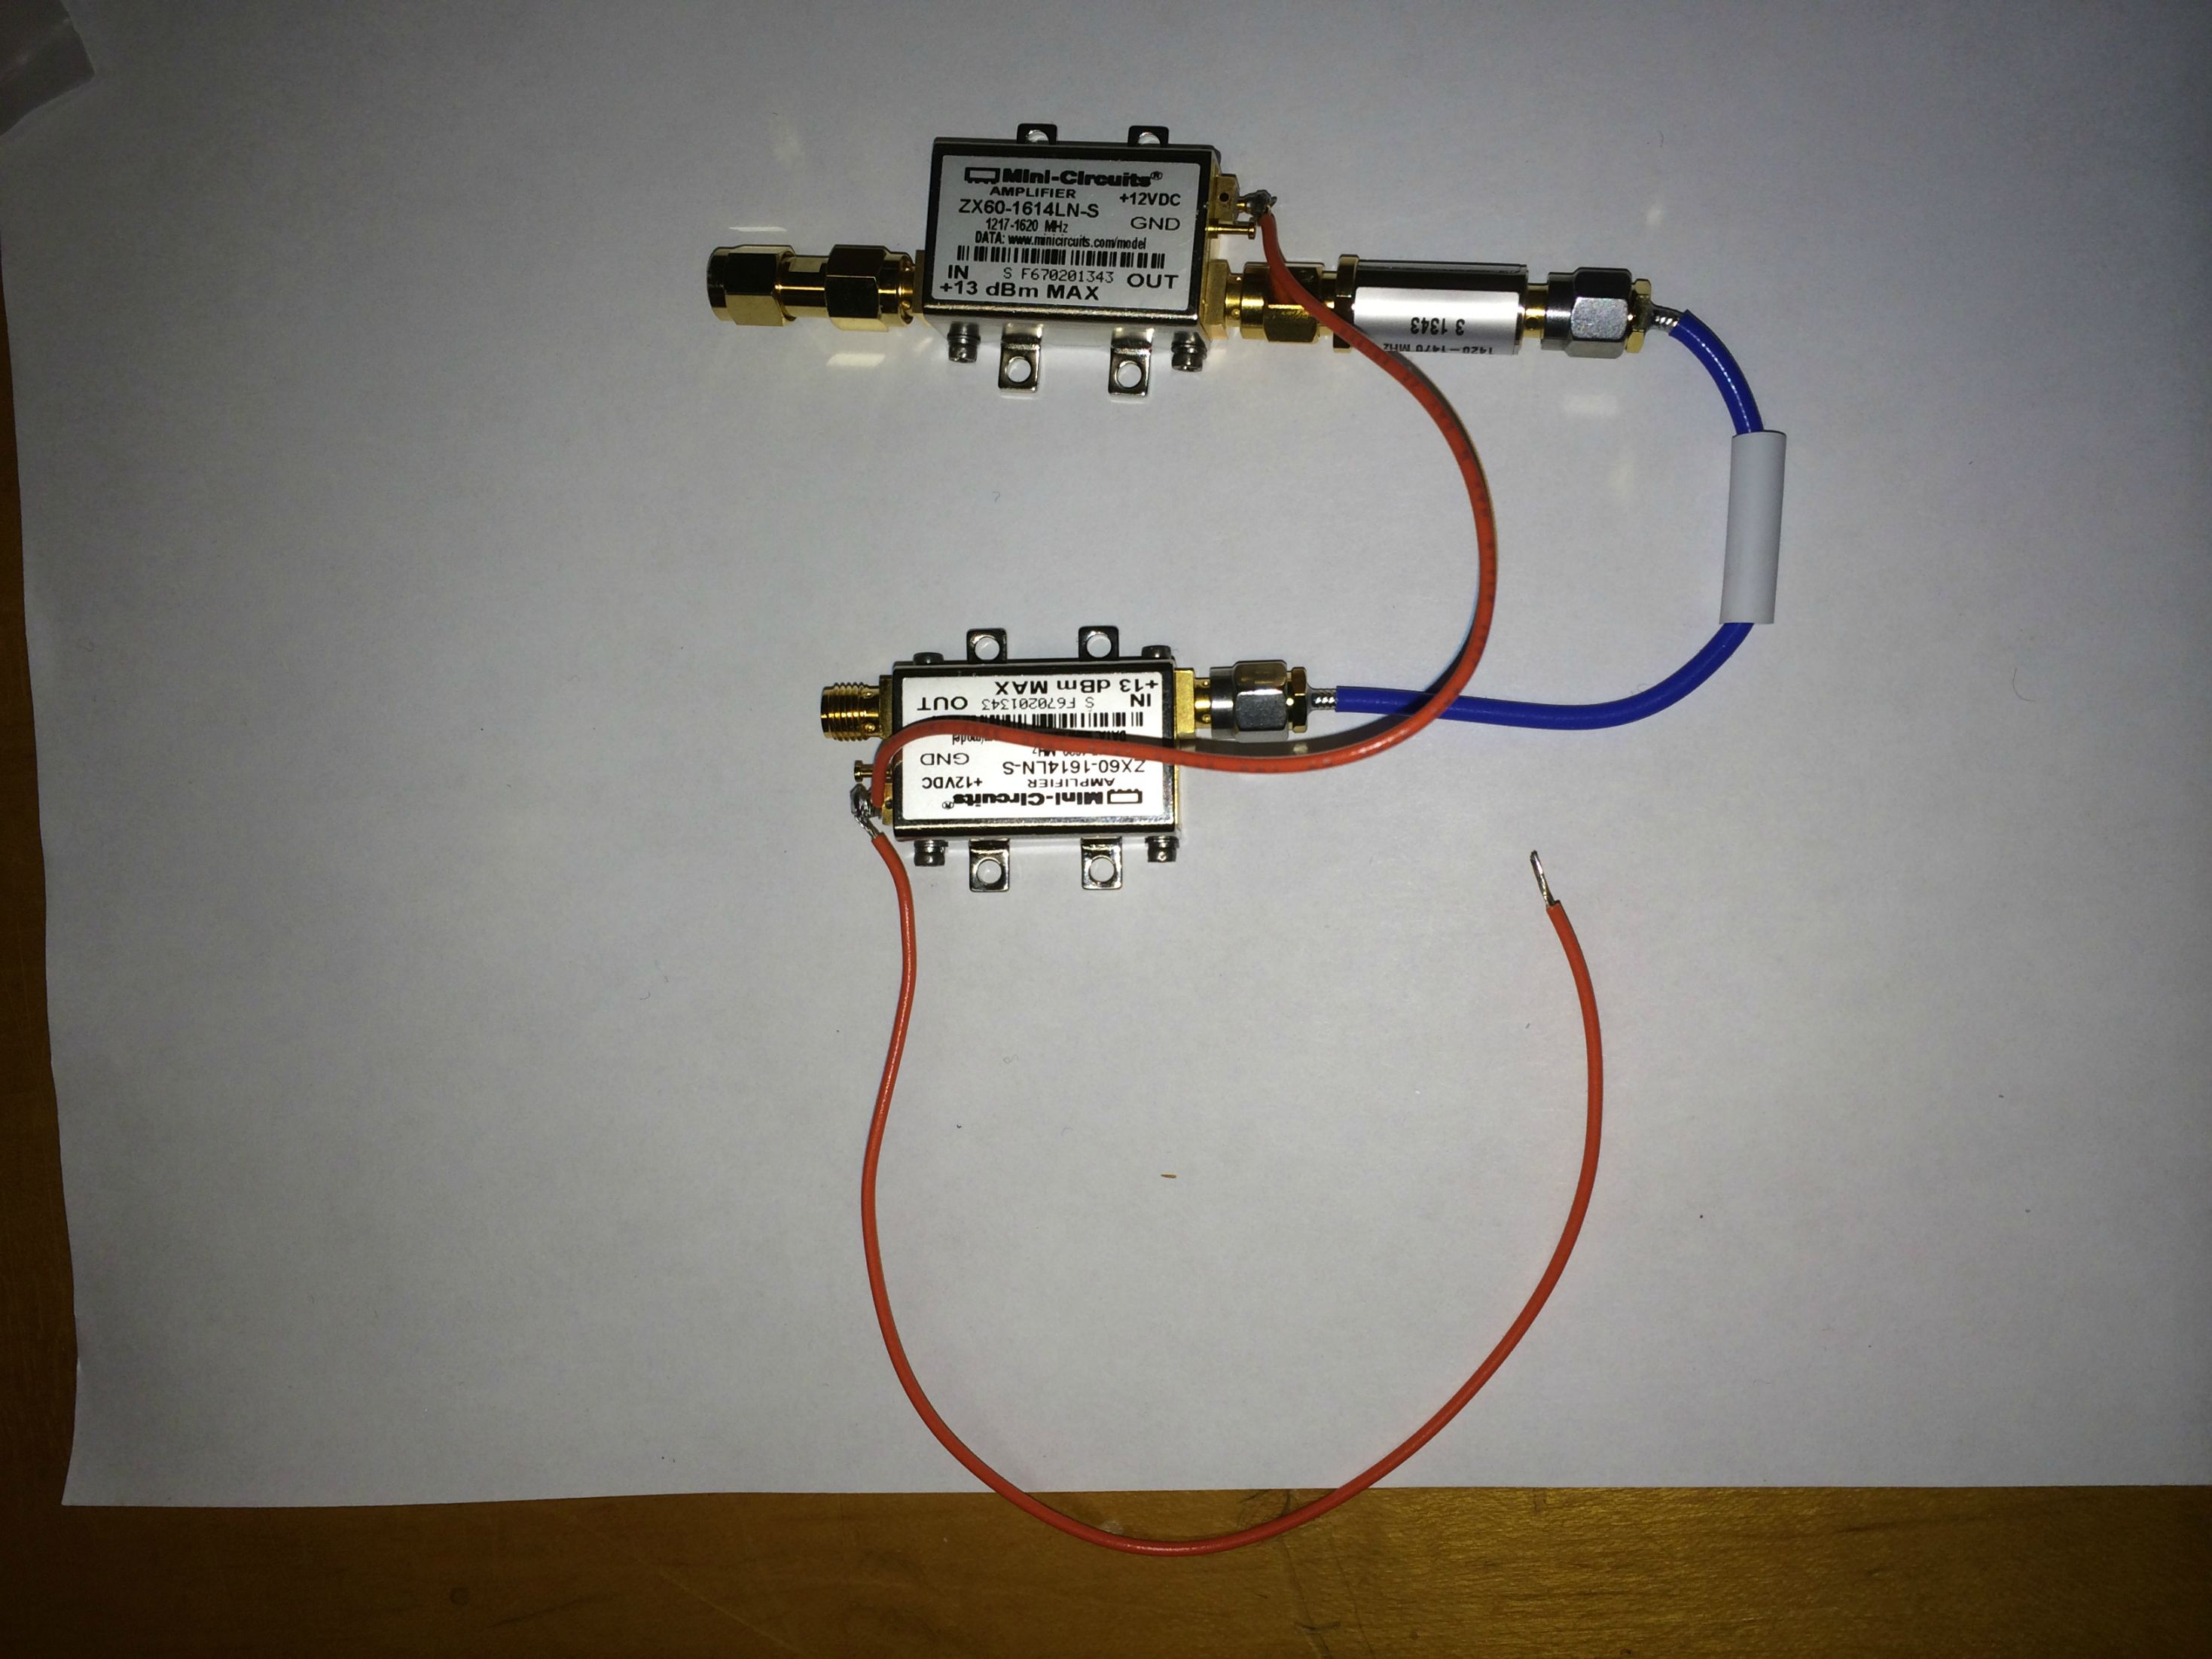
\includegraphics[scale=0.13]{lna/04.jpeg}
\end{center}

Soldered the other end of the second wire to the 12 volt pin on the bias tee.
Connected "RF" side of the bias tee and "out" side of Amp 2 with coaxial cable. 

\begin{center}
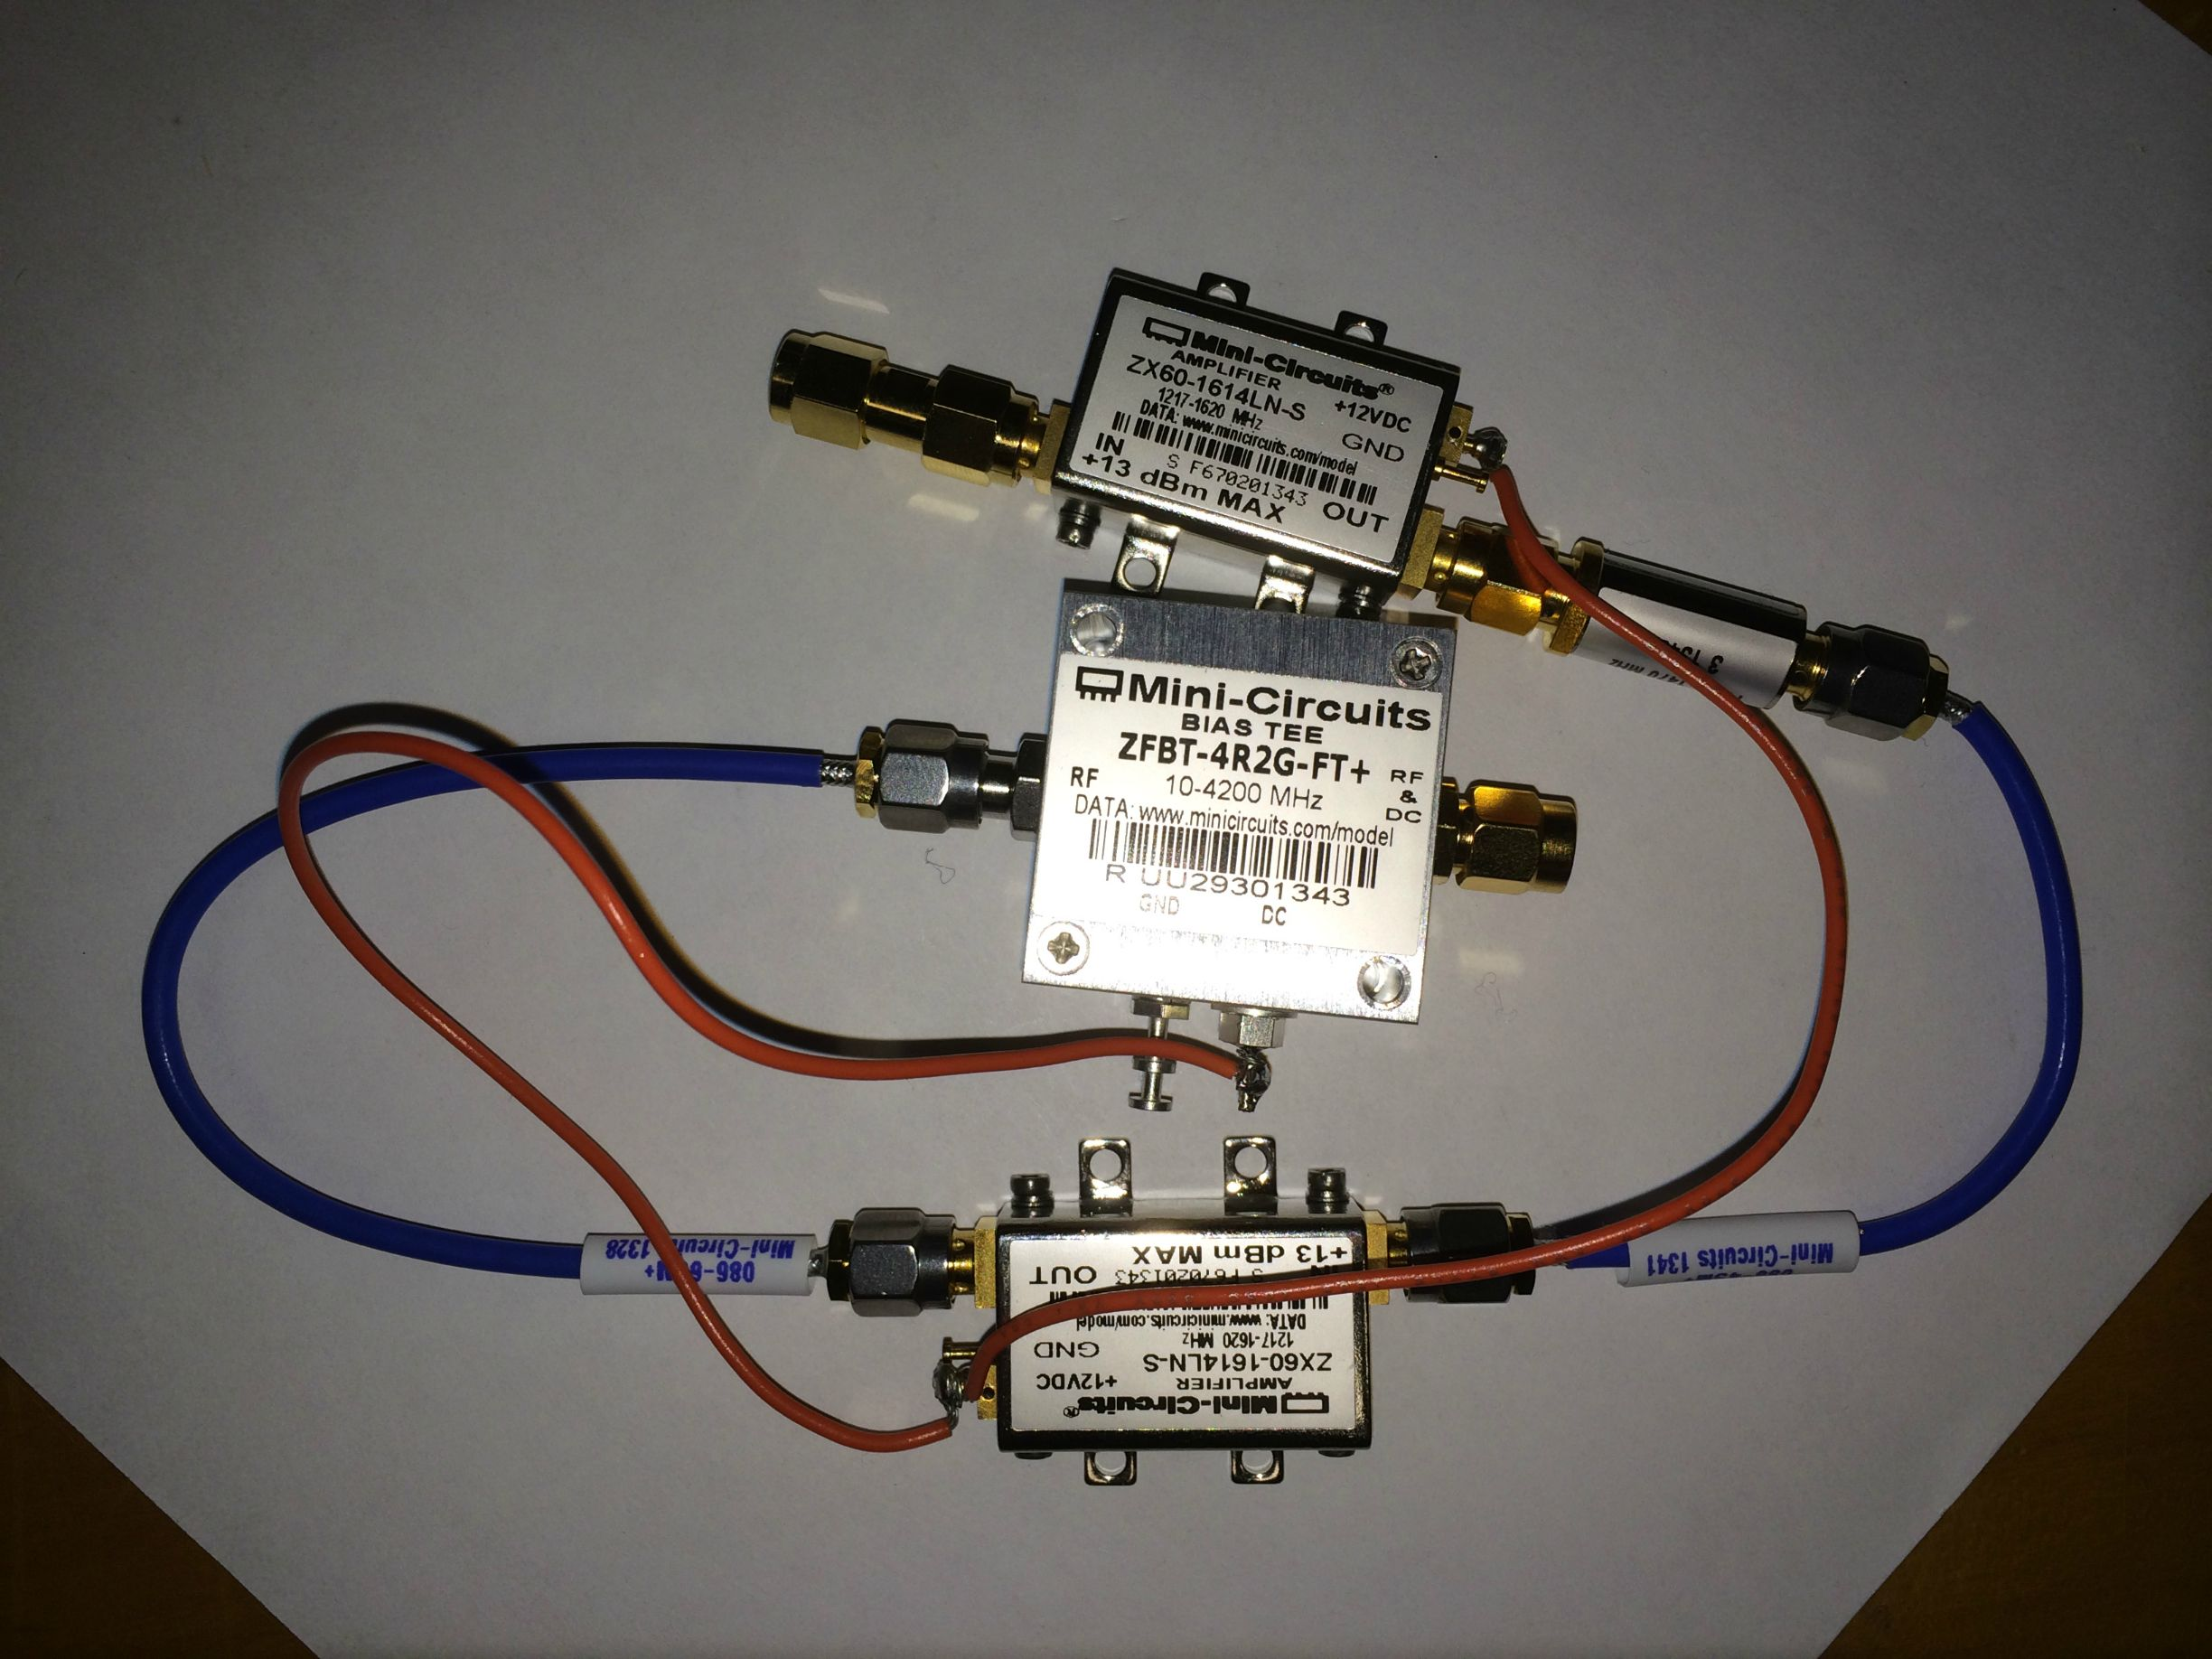
\includegraphics[scale=0.15]{lna/05.jpeg}
\end{center}

Placed this group into the case, with coupler and "RF DC" side of the bias tee protruding from the holes. 

\begin{center}
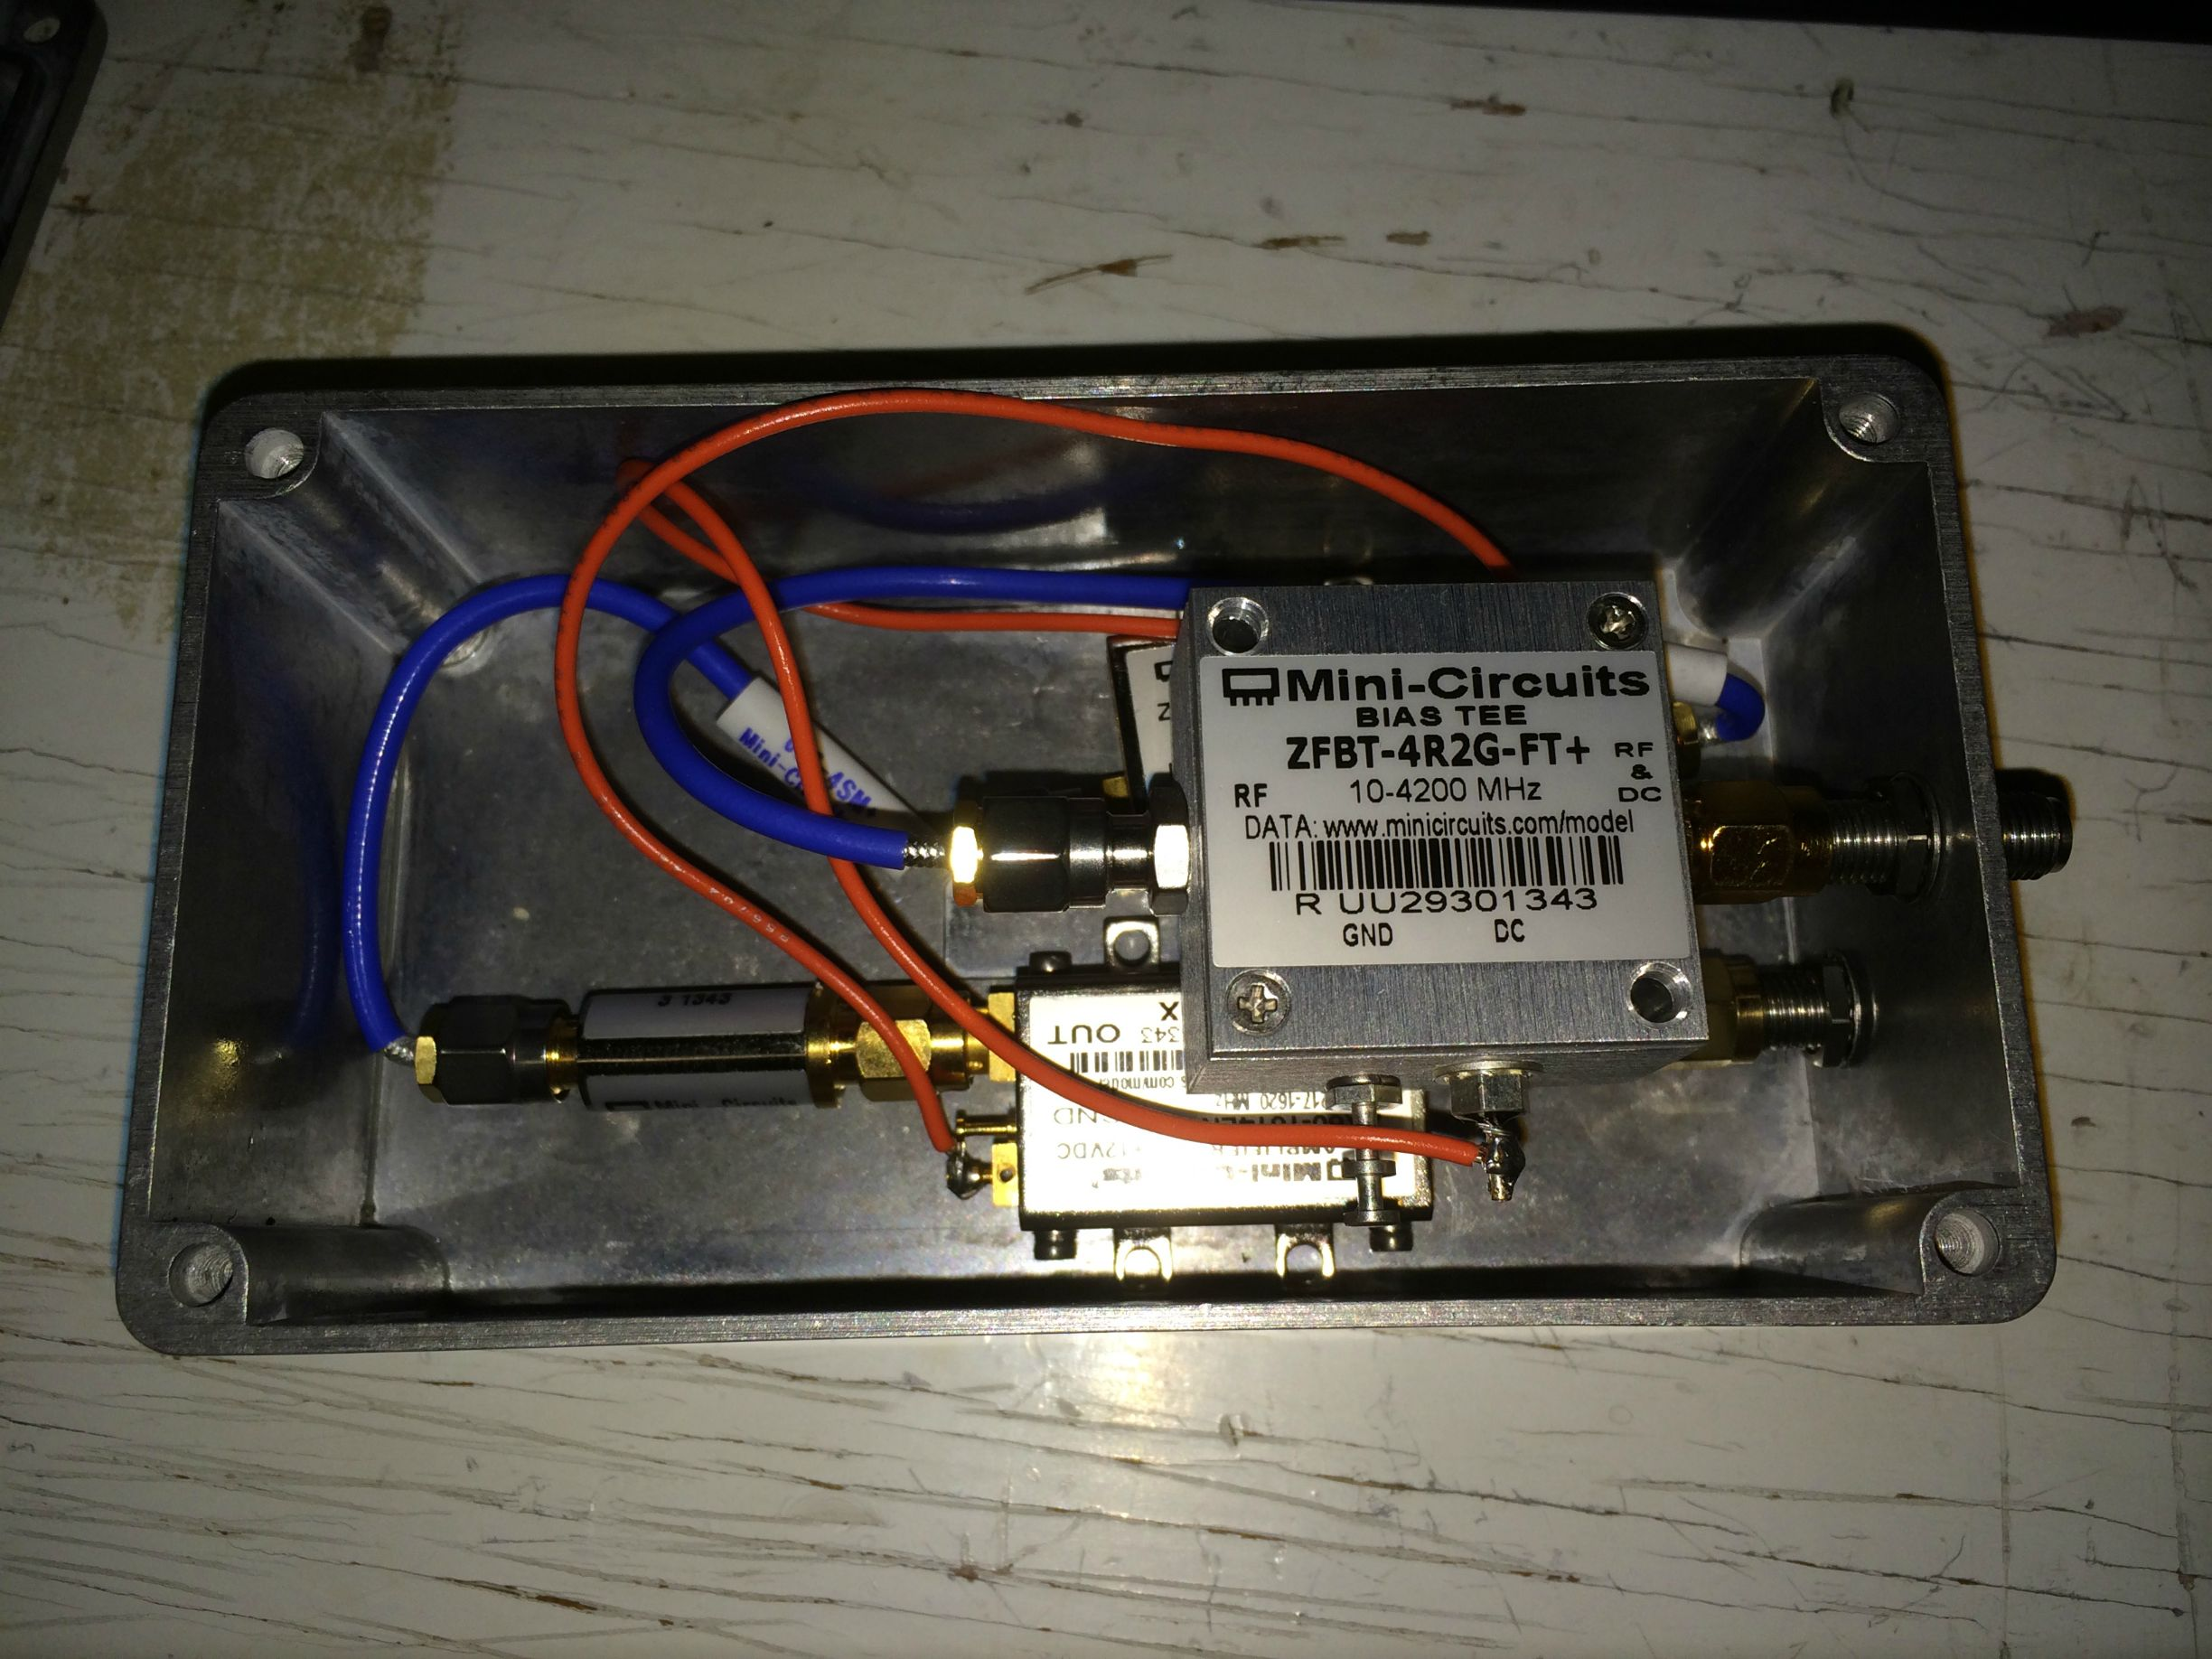
\includegraphics[scale=0.12]{lna/06.jpeg}
\end{center}

Placed on rubber lining, and case cover, wrote LNA on top, and screwed into place. 

\begin{center}
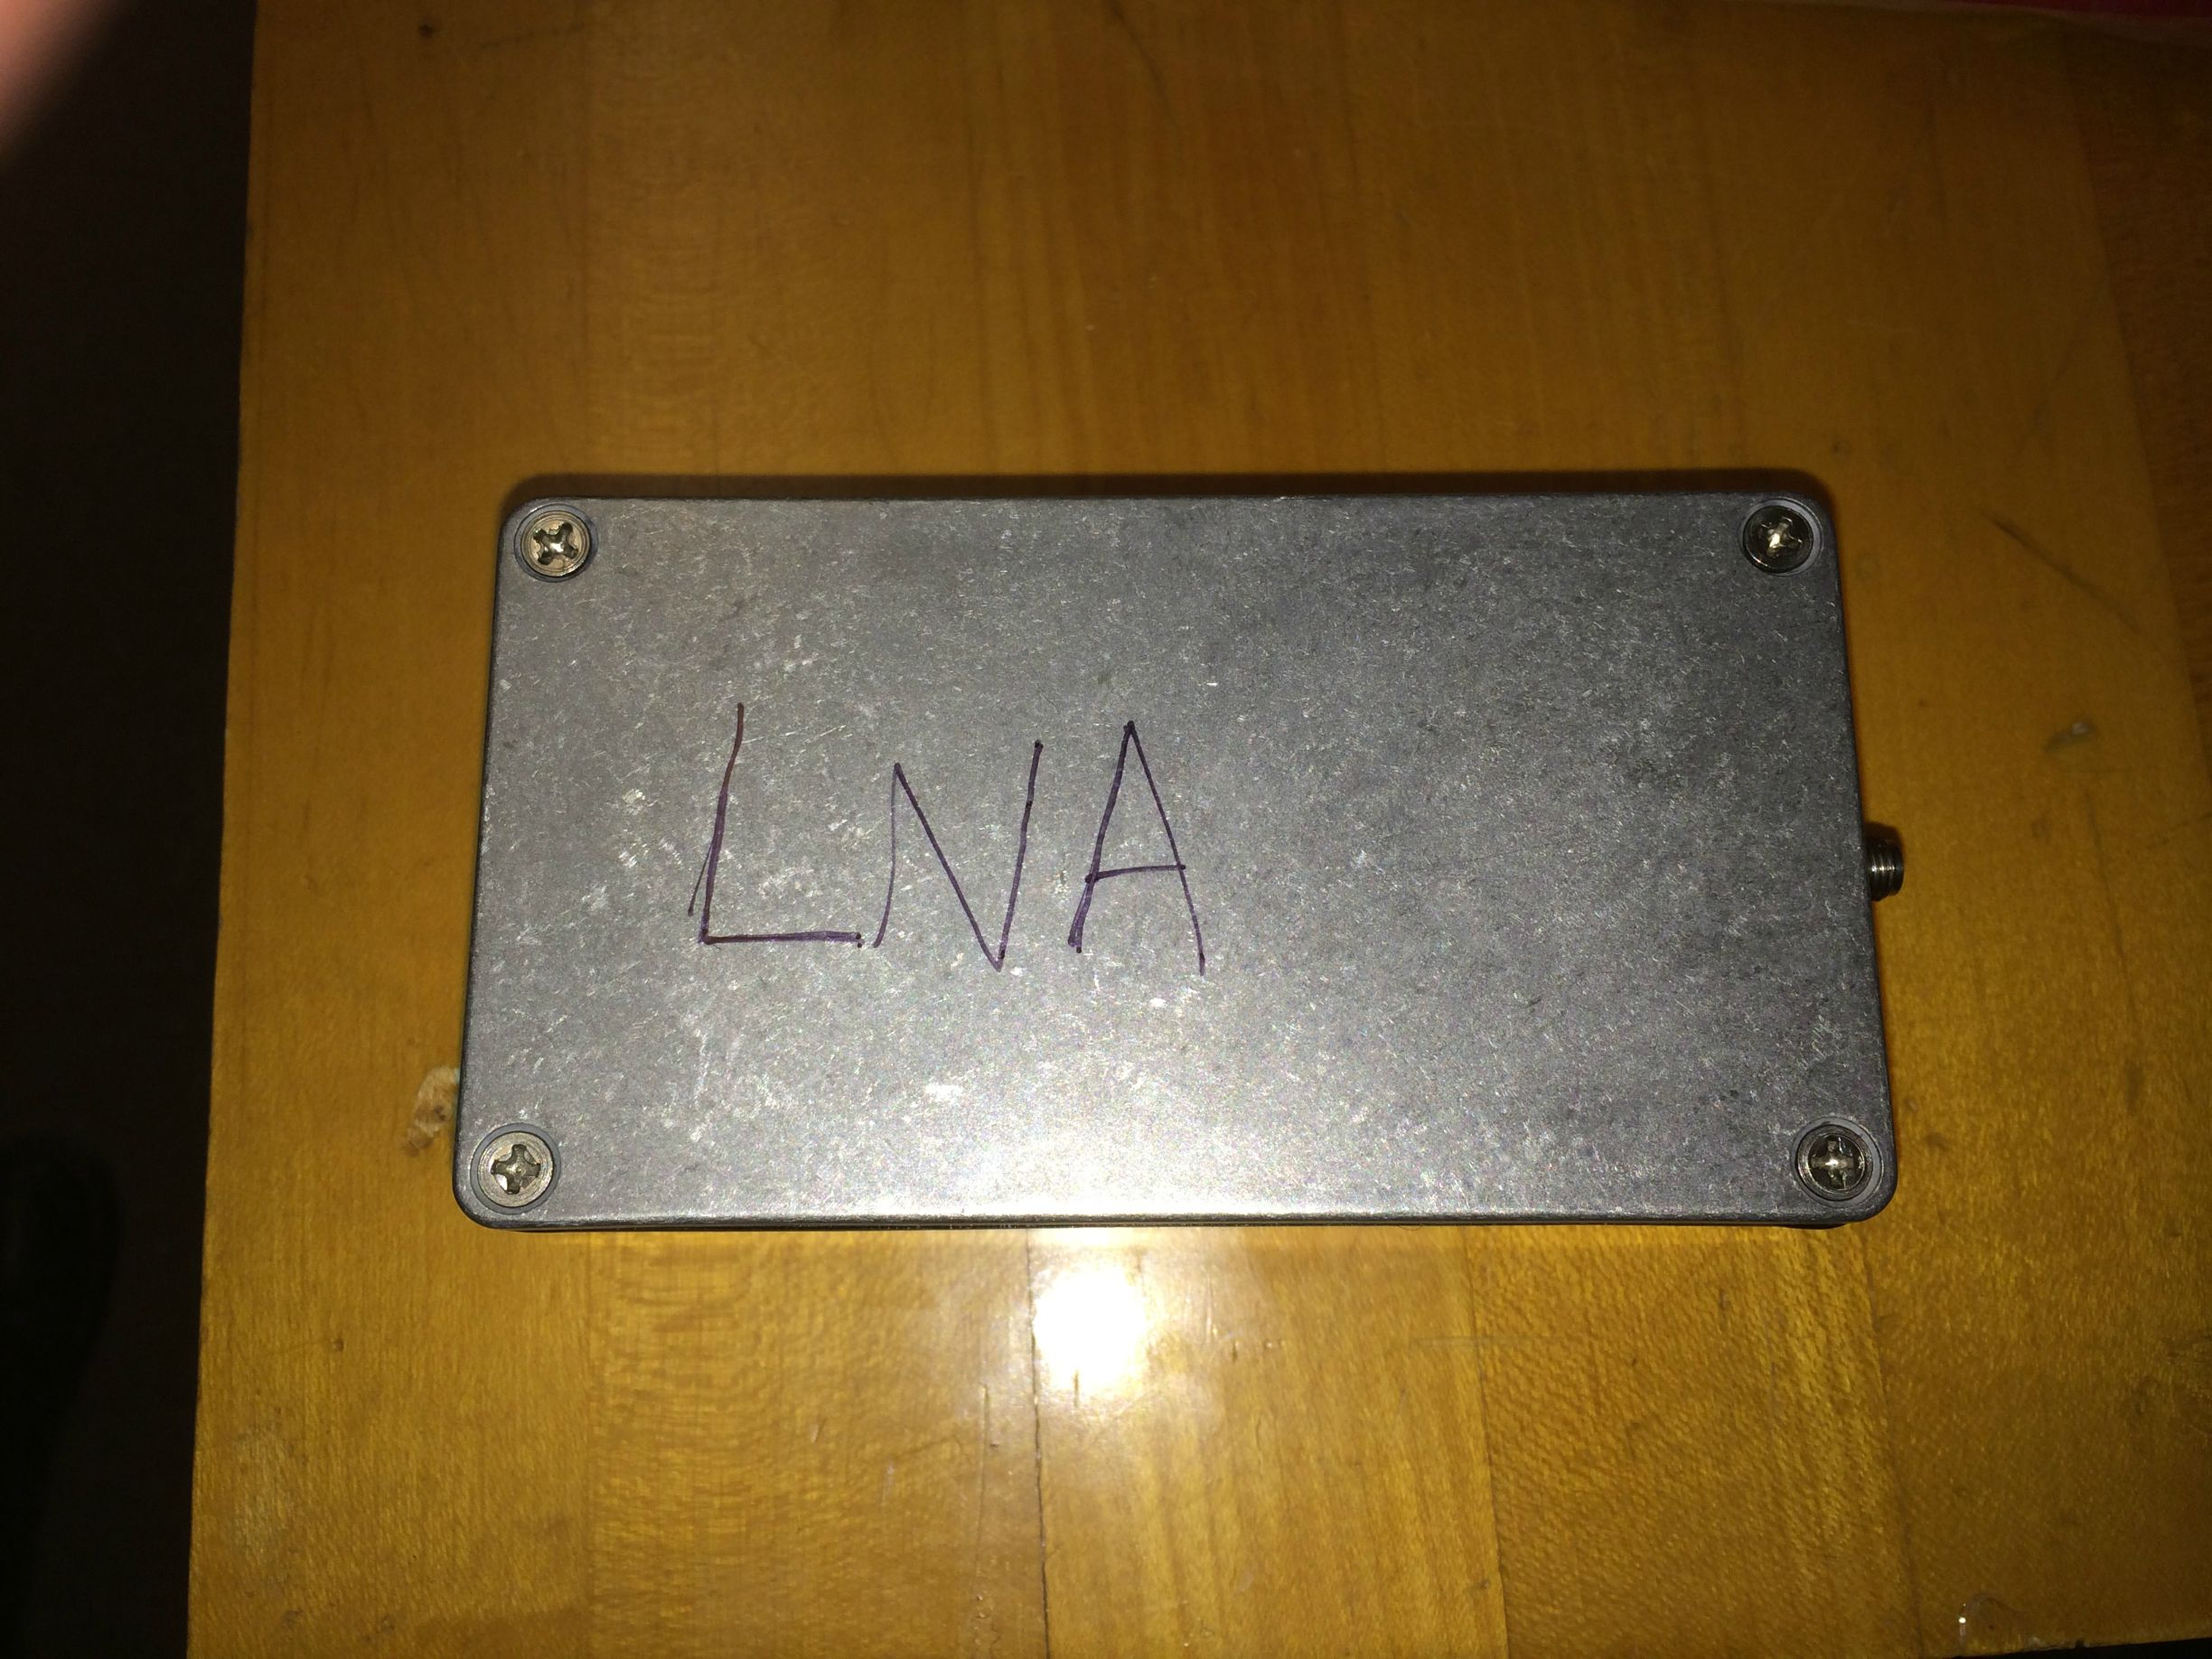
\includegraphics[scale=0.12]{lna/07.jpeg}
\end{center}

Pics of assembly of dc jack connector to f type coax adapter.
Solder middle pin of dc plug connector to perf board.
Solder middle pin of f type plug connector to same conductive strip of perf board. 

\begin{center}
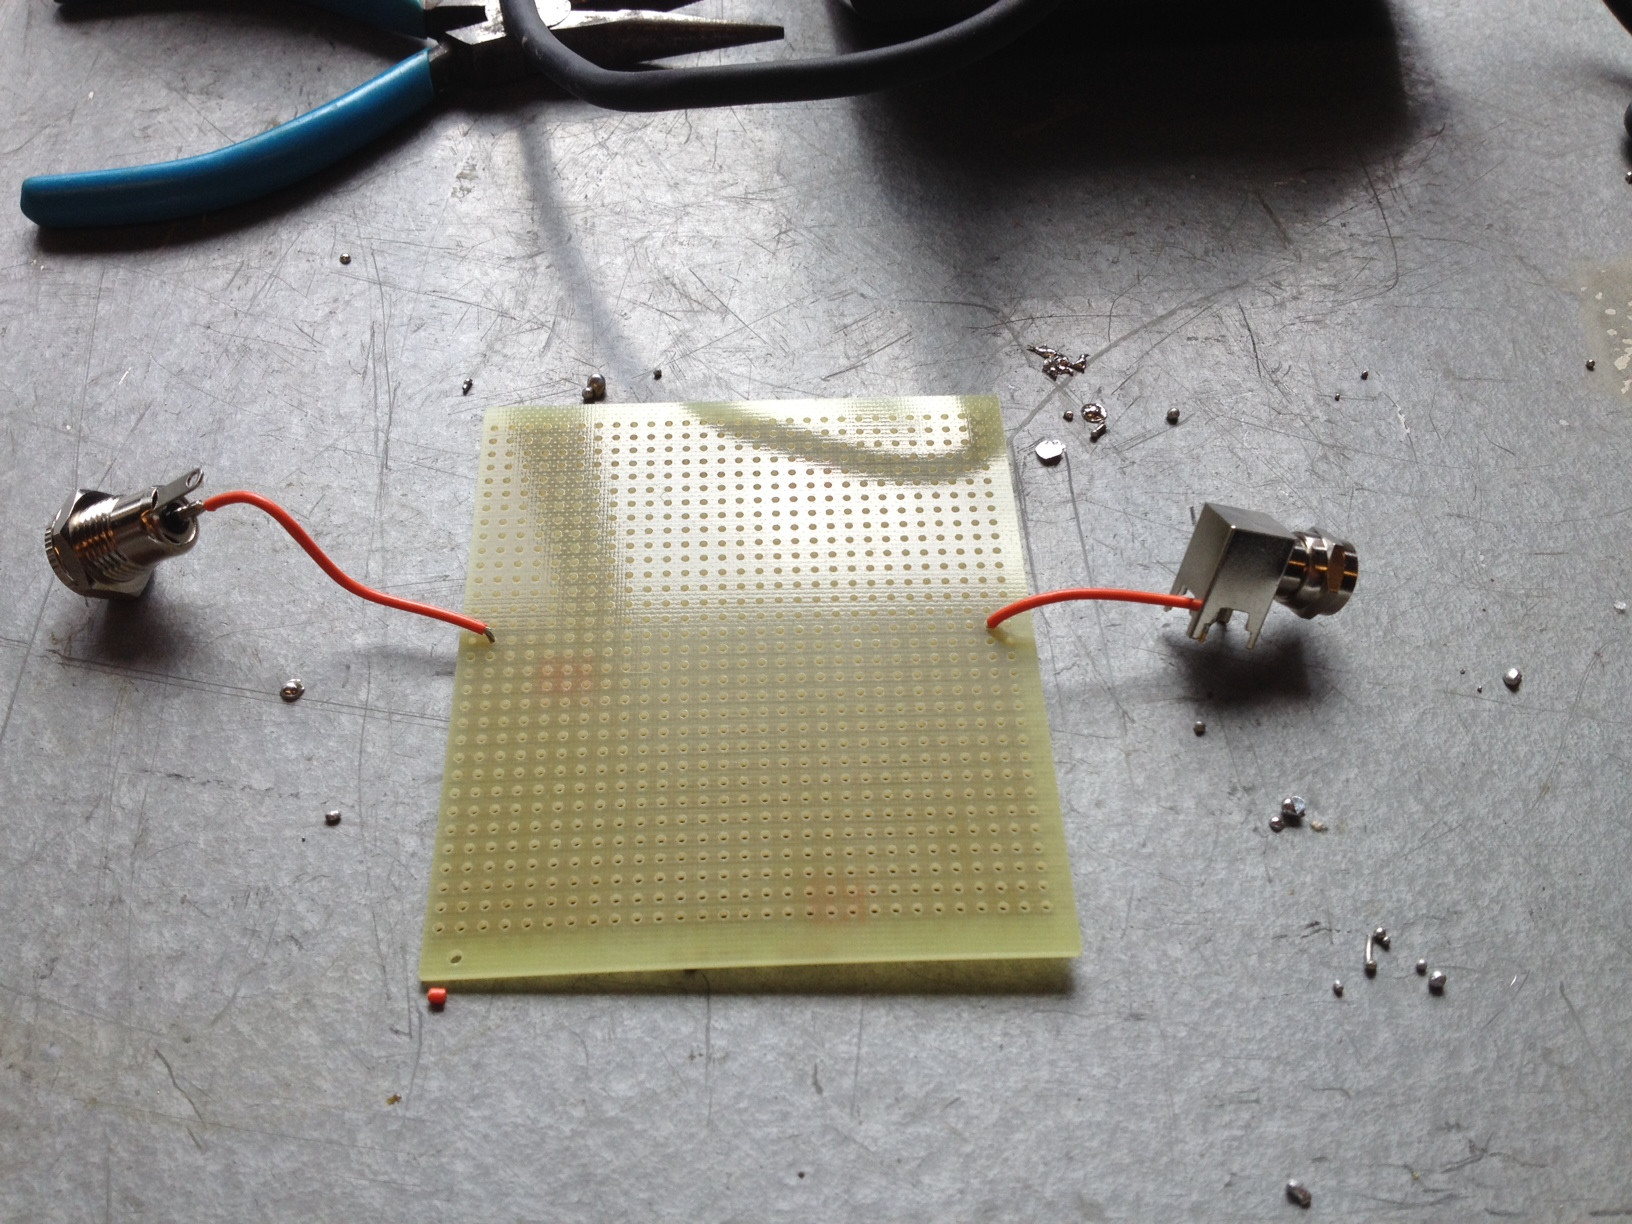
\includegraphics[scale=0.20]{lna/08.jpeg}
\end{center}

Under side. 

\begin{center}
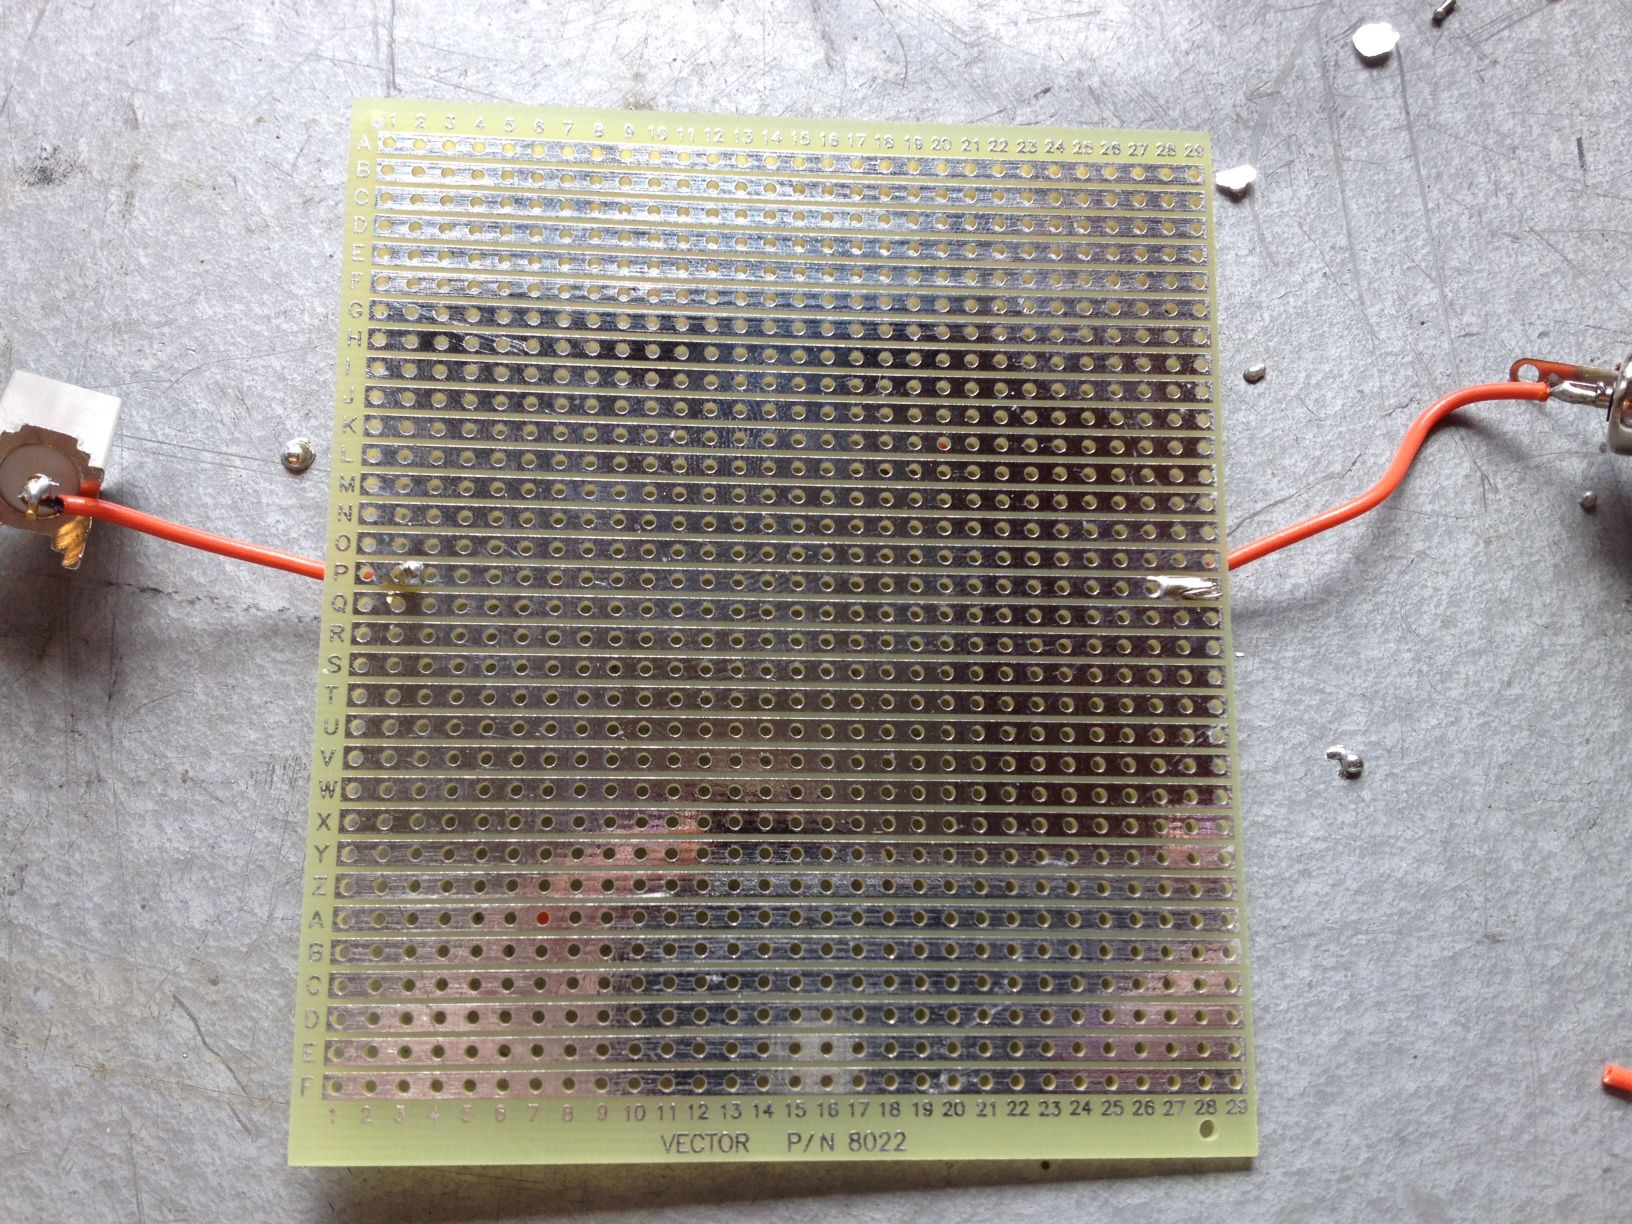
\includegraphics[scale=0.20]{lna/09.jpeg}
\end{center}

Solder ground pin on dc jack connector directly to one of the ground pins on the f type plug connector. 

\begin{center}
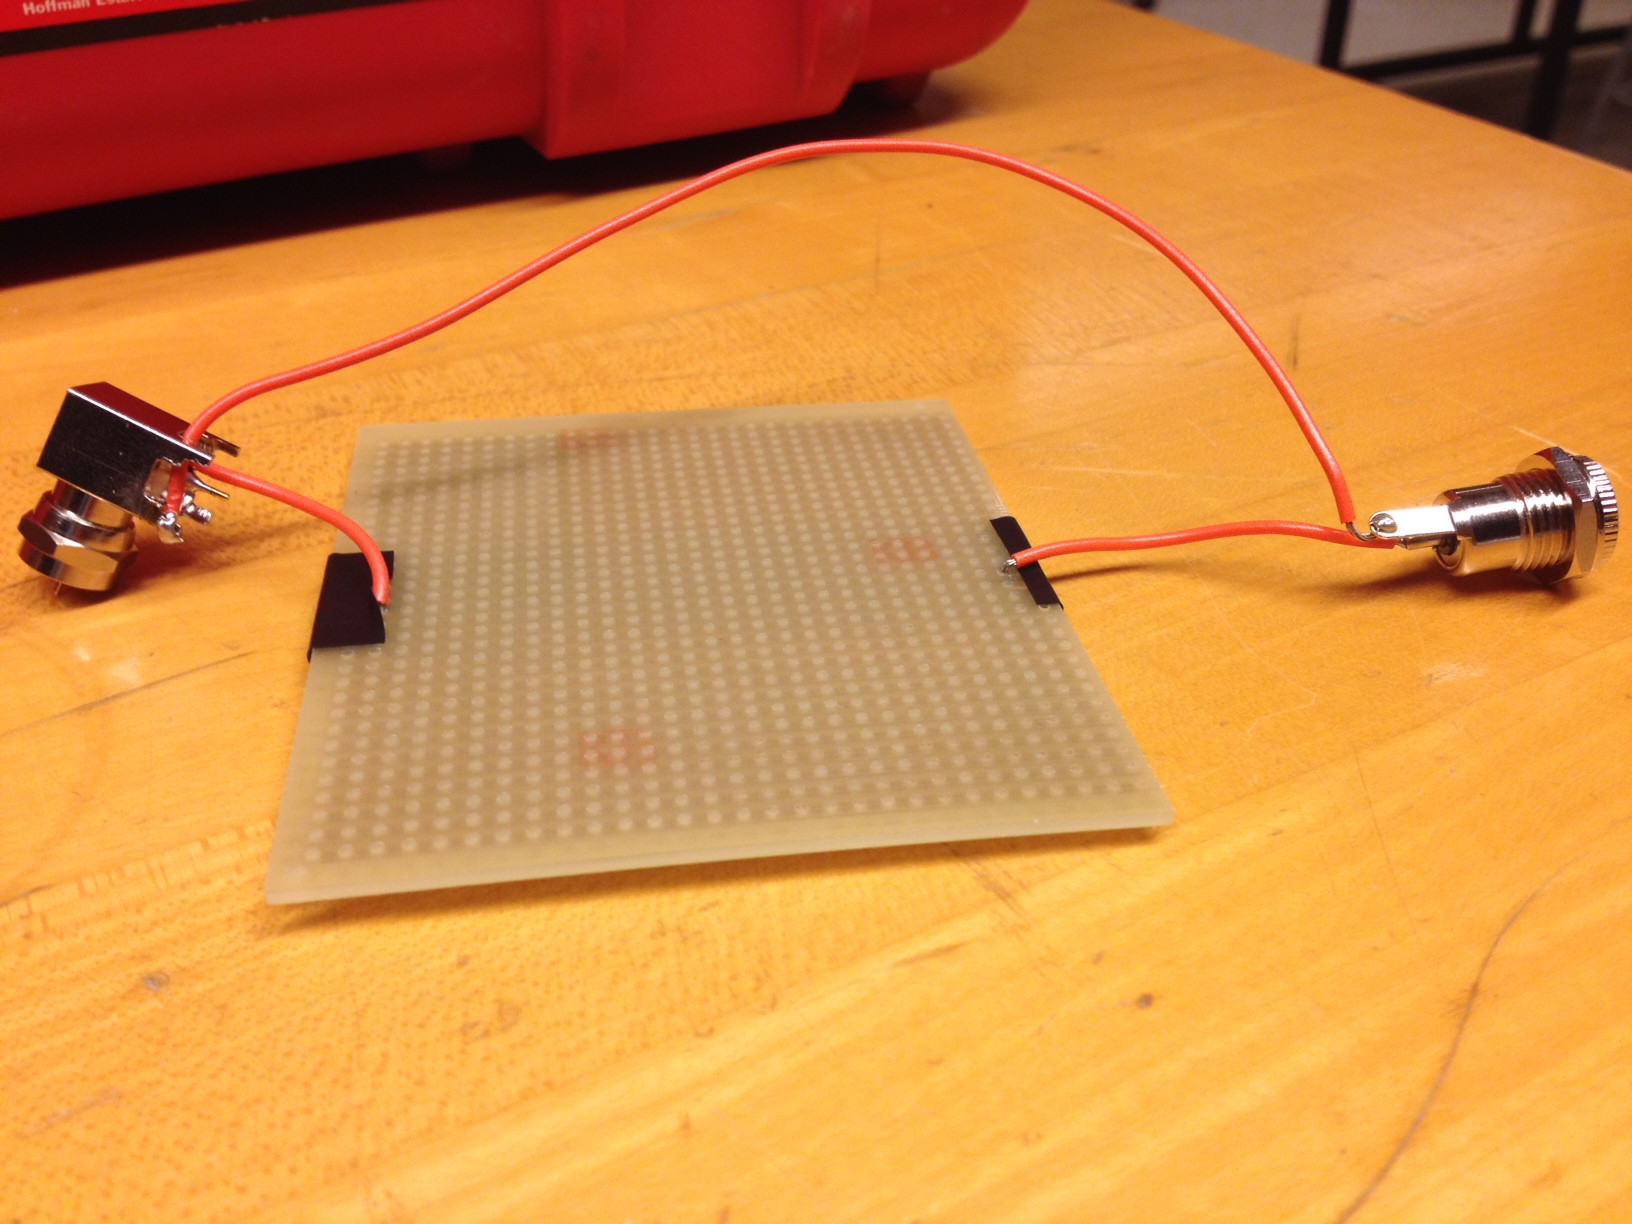
\includegraphics[scale=0.20]{lna/10.jpeg}
\end{center}

Back End b/t Dongle and LNA Put Together 

\begin{center}
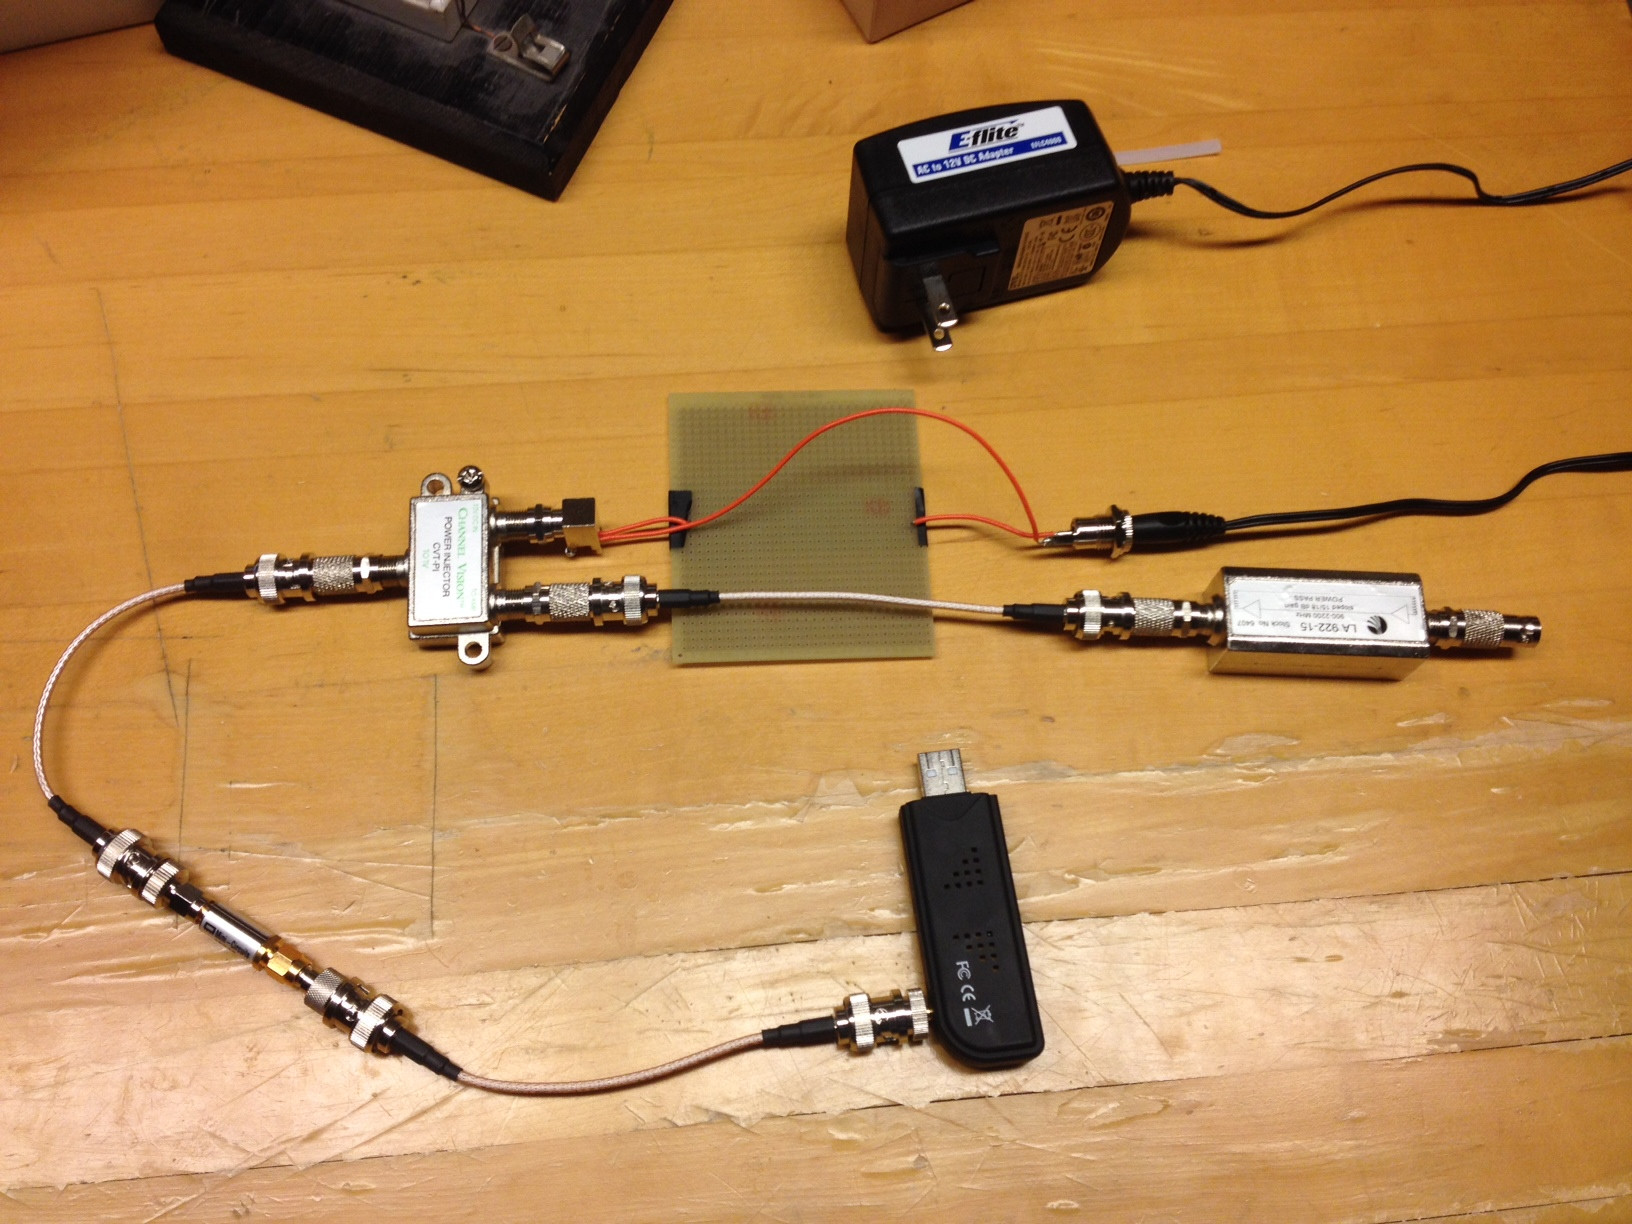
\includegraphics[scale=0.20]{lna/11.jpeg}
\end{center}



%%%%%%%%%%%%%%%%%%%%%%%%%%%%%%%%%%%%%%%%
\subsection{Building LNA to Dongle Interface}

\begin{center}
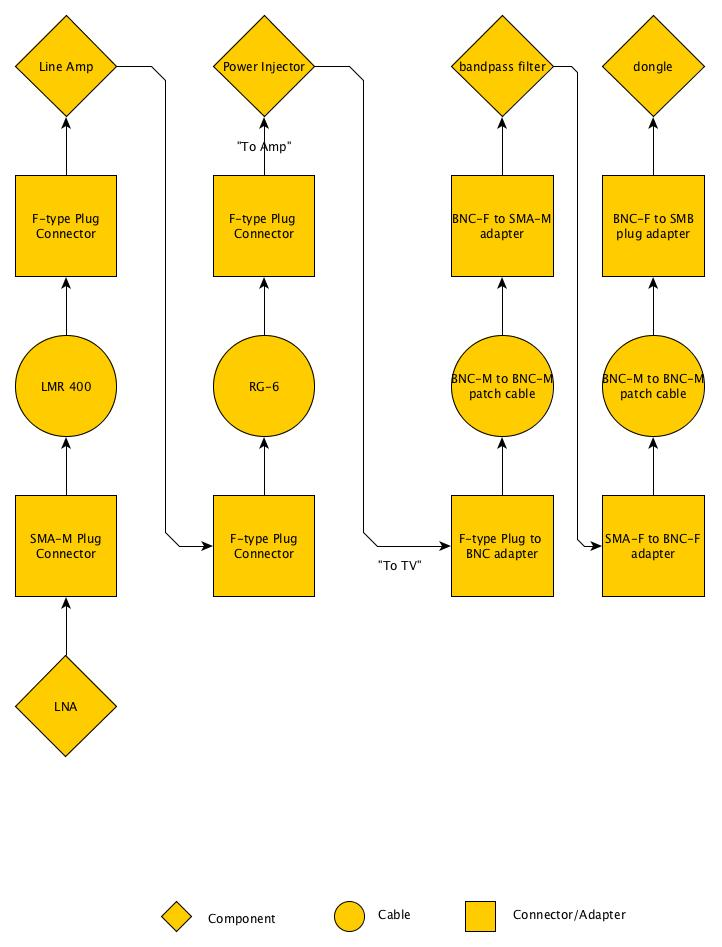
\includegraphics[scale=0.35]{lnainterface/01.jpeg}
\end{center}


\subsubsection{Parts Needed}

\begin{itemize}
\item 4 BNC jack (female) to BNC jack patch cables
\item Line Amp
\item Power Injector
\item (DIY) DC plug (male) to F-type Plug adapter
\item 1 SMA-M to BNC-M adapter
\item 1 SMA-F to BNC-M adapter
\item 5 F-type plug to BNC-M adapters
\item Perf board/breadboard
\item 22-gauge copper wire
\item DC-Barrel jack connector
\item Right-angle F-type plug connector
\end{itemize}

\subsubsection{Tools Needed}

\begin{itemize}
\item Soldering Iron + Solder
\item Wire cutters/strippers
\item Electrical Tape
\end{itemize}

\subsubsection{Building DC Barrel Jack to F-Type Plug Connector}

\begin{itemize}
\item Assemble the perf board/breadboard, dc barrel jack connector, F-type plug connector, and copper wire.
\item Solder middle pin of dc plug connector to perf board.
\item Solder middle pin of f type plug connector to same conductive strip of perf board. 
\end{itemize}

\begin{center}
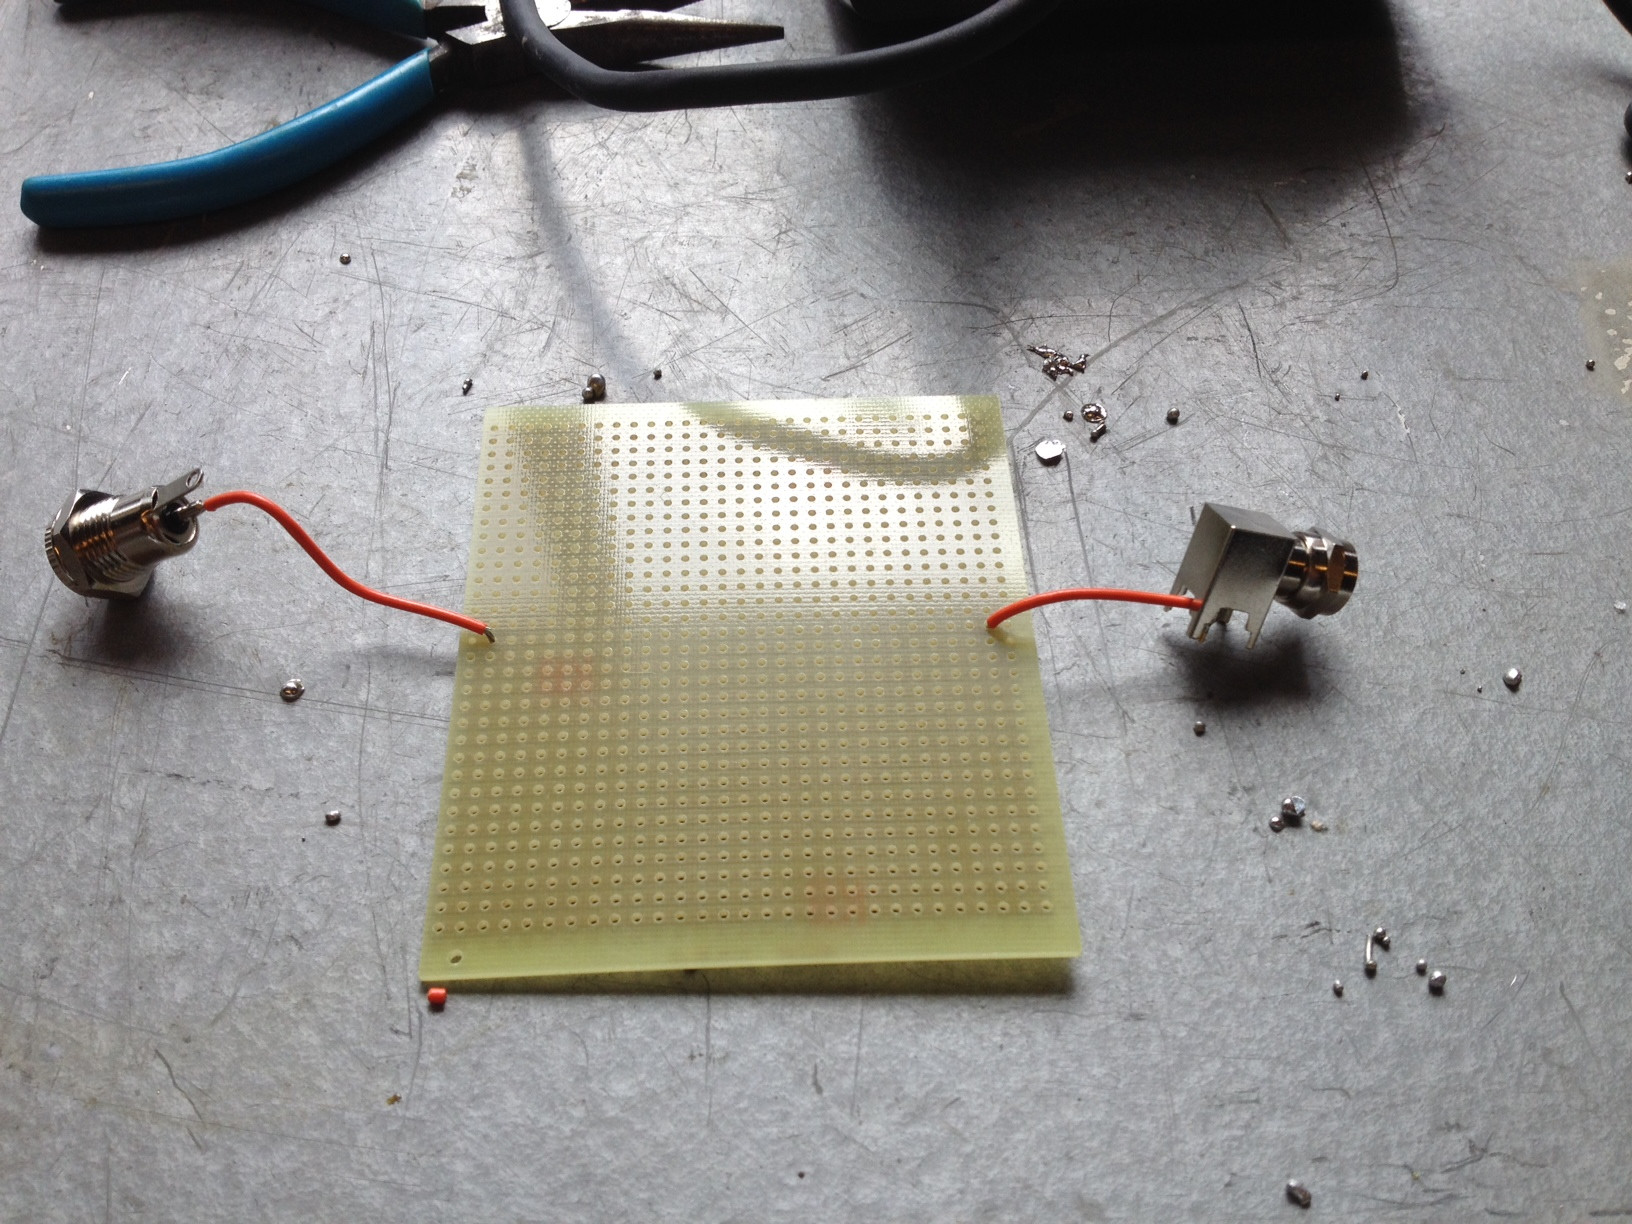
\includegraphics[scale=0.20]{lnainterface/02.jpeg}
\end{center}

Under side:

\begin{center}
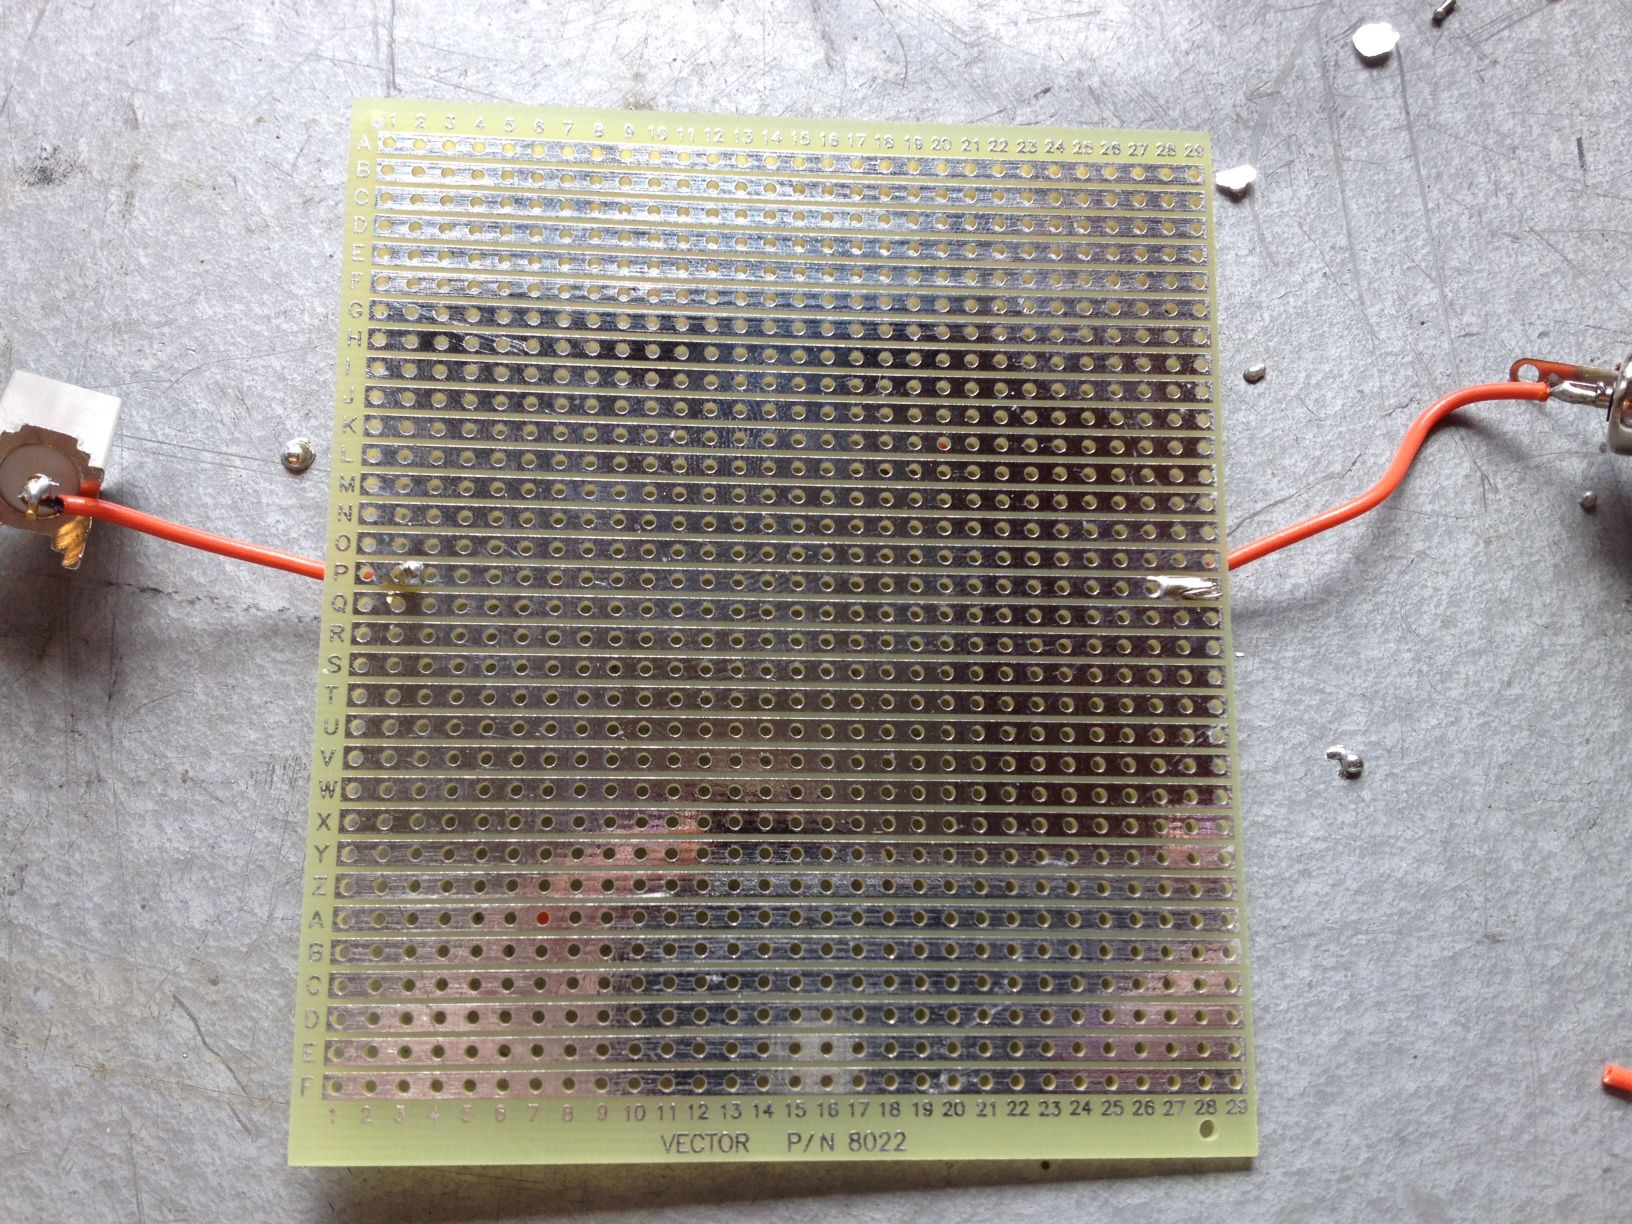
\includegraphics[scale=0.20]{lnainterface/03.jpeg}
\end{center}

Solder ground pin on dc jack connector directly to one of the ground pins on the f type plug connector. 

\begin{center}
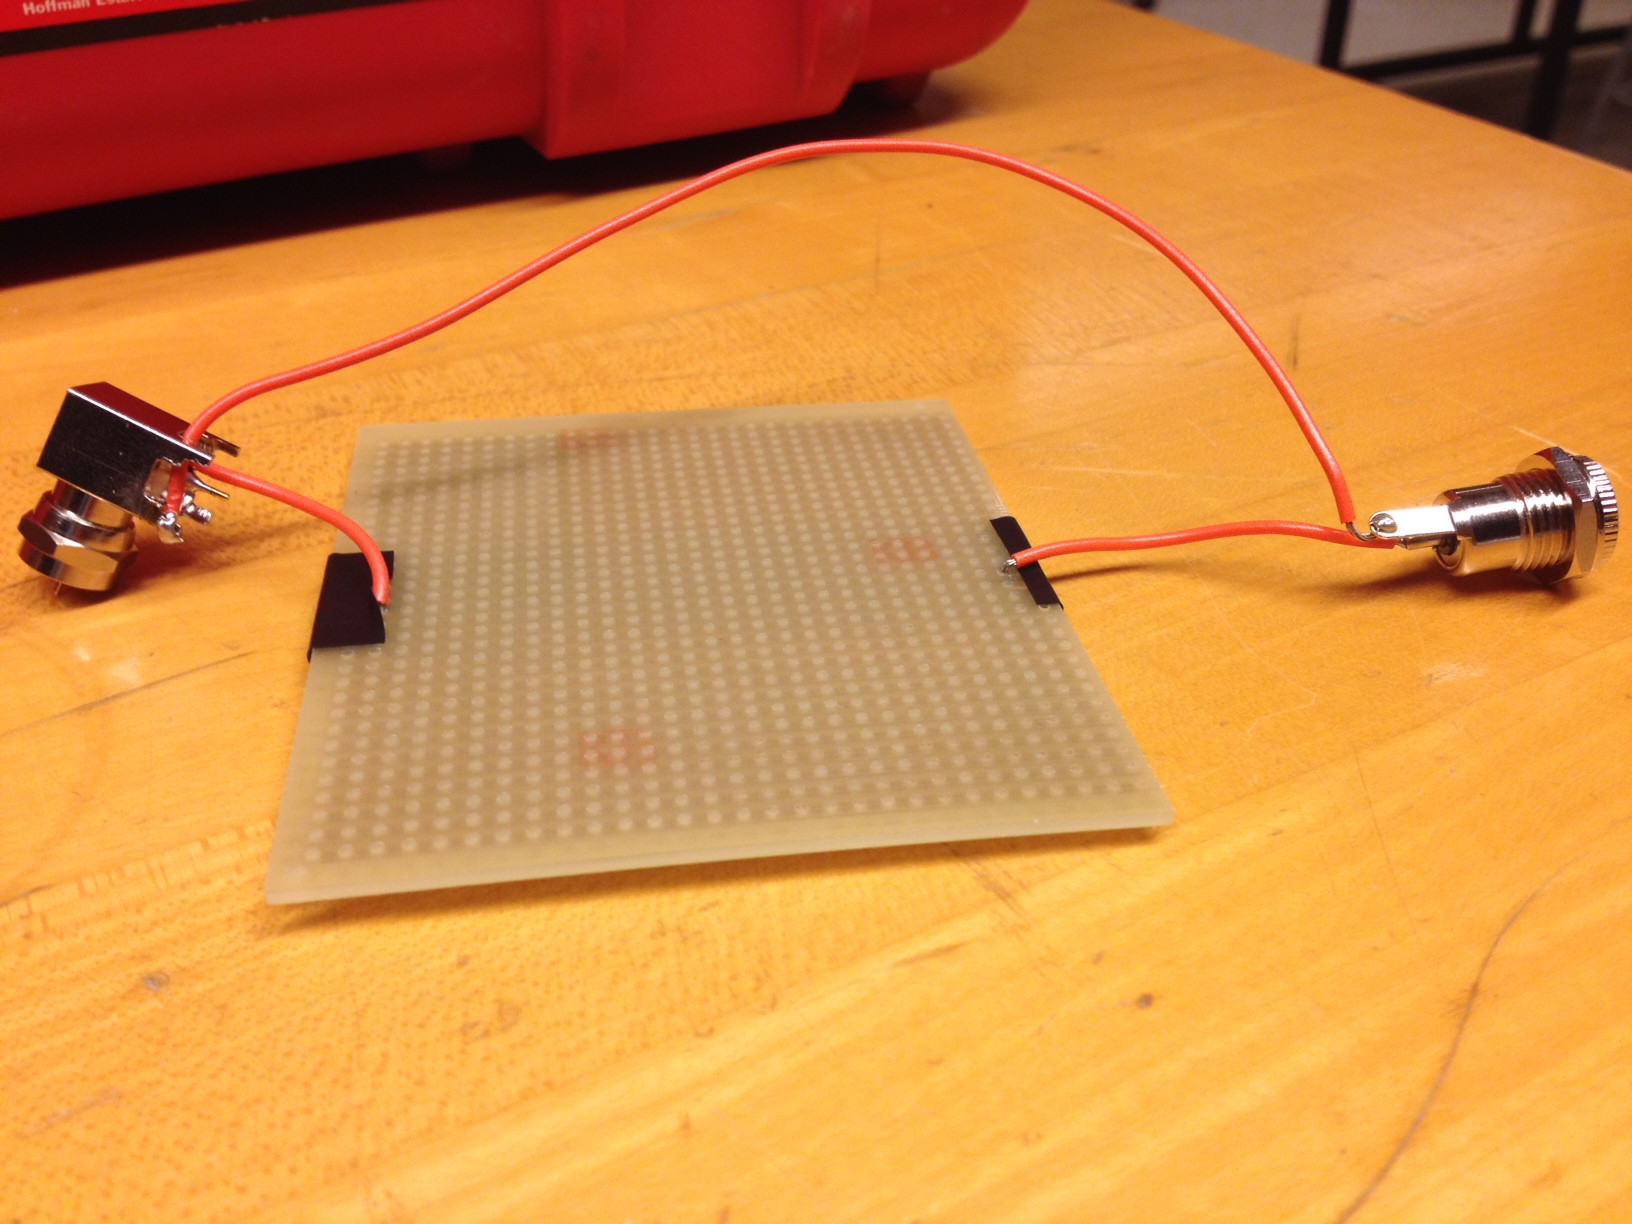
\includegraphics[scale=0.20]{lnainterface/04.jpeg}
\end{center}

\subsubsection{Assembly}

\begin{itemize}
\item Attach one F type plug to BNC-M adapter to one end of one of the patch cables.
\item To the other end of the patch cable, attach another F-type plug to BNC-M adapter.
\item To the F-type side of the adapter, attach the "in" side of the line amp.
\item To the "out" side of the line amp, attach another F-type plug to BNC-M adapter.
\item Attach another patch cable to the BNC side of the adapter.
\item To the other end of the patch cable, attach another F-type plug to BNC-M adapter.
\item Plug the F-type side of the adapter into the "to amp" input on the Power Injector.
\item Screw an F-type plug to BNC-M adapter onto the "out" of the power injector.
\item Attach another patch cable to the adapter.
\item Onto the free side of the patch cable, screw on your SMA-M to BNC-M adapter.
\item Attach the "in" of the bandpass filter to the free (SMA-M) side of the adapter.
\item To the "out" of the BPF, screw in the SMA-F side of the SMA-F to BNC-M adapter.
\item Attach another patch cable to the previous adapter.
\item Attach the BNC-M to SMB-M adapter to the patch cable.
\item Plug the SMB-M side of your adapter into the dongle.
\item Into the "12V DC IN" portion of the power injector, screw the F-type side of the dc plug to F type adapter
\item Plug your 12V DC wall wart power supply into the DC Barrel Jack side of your DIY adapter.
\item Plug dongle into computer.
\end{itemize}

\begin{center}
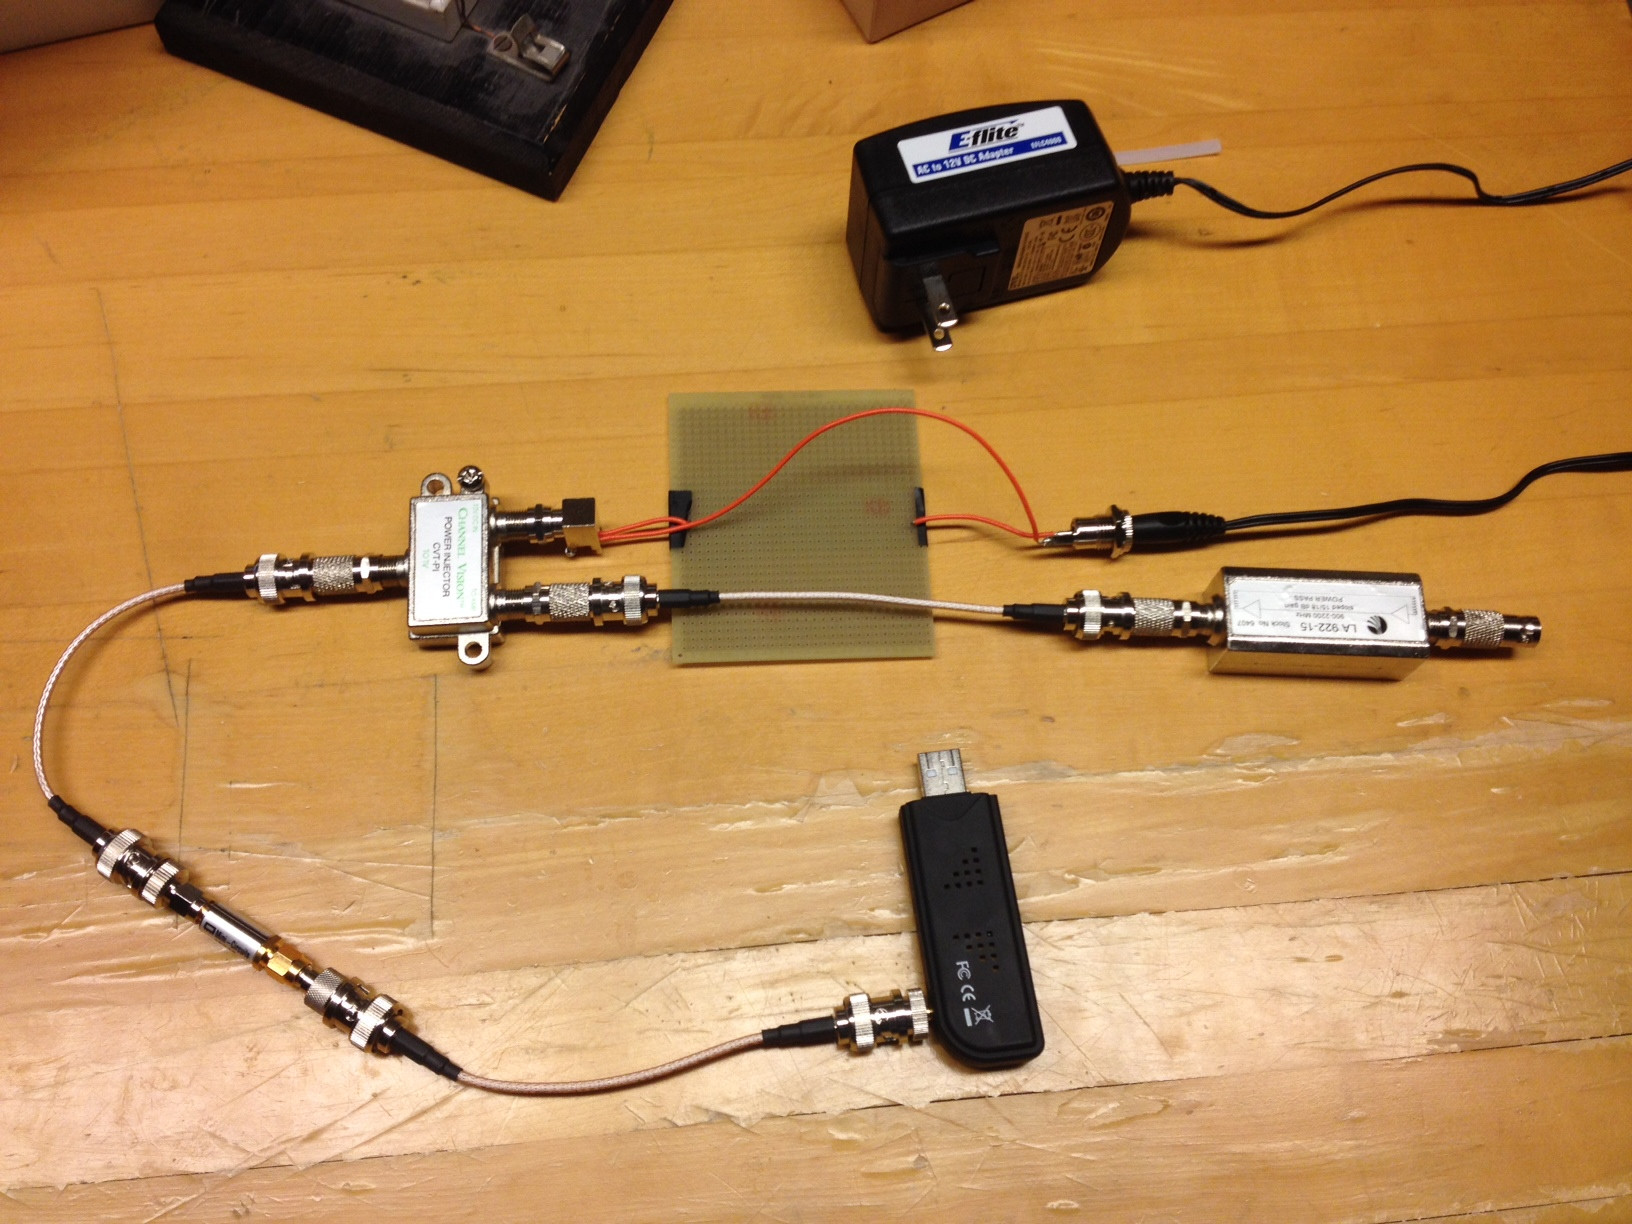
\includegraphics[scale=0.20]{lnainterface/05.jpeg}
\end{center}

\begin{center}
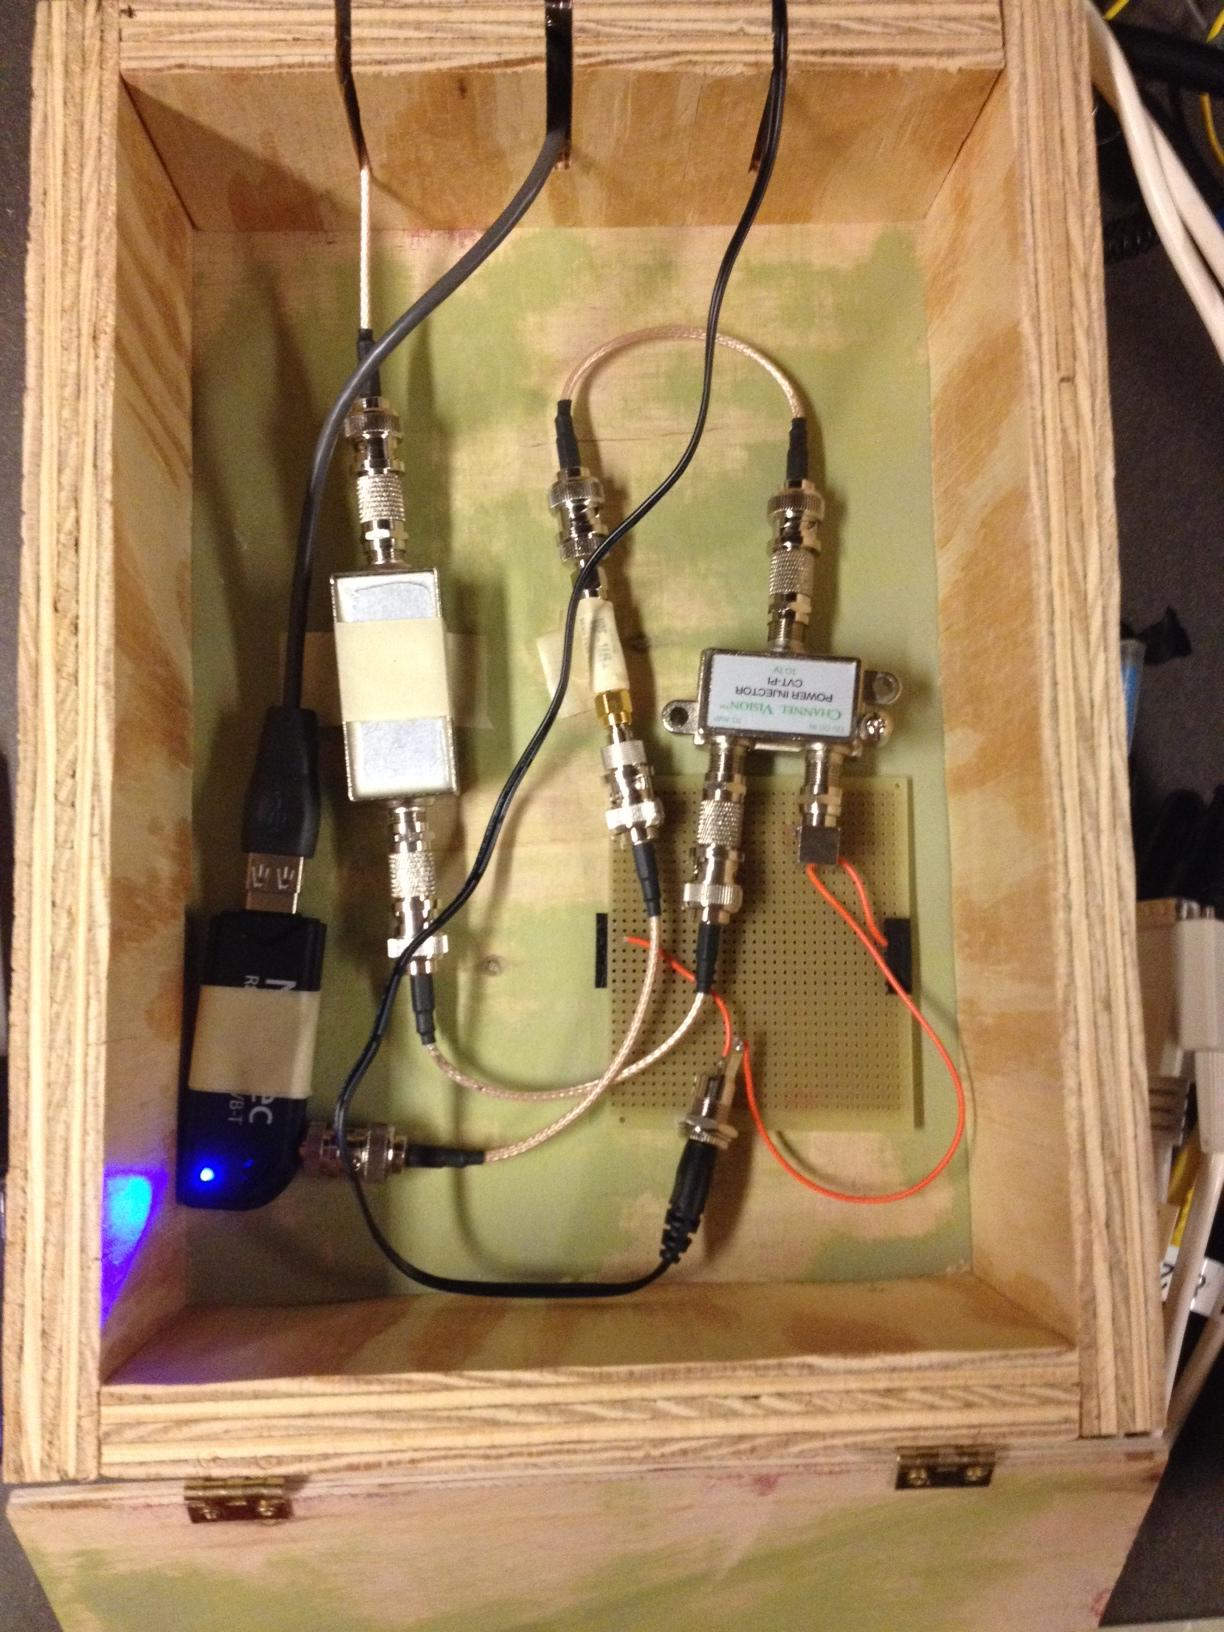
\includegraphics[scale=0.20]{lnainterface/06.jpeg}
\end{center}


%%%%%%%%%%%%%%%%%%%%%%%%%%%%%%%%%%%%%%%%

\subsection{Feed}

\subsubsection{Cutting Styrofoam Rod}
We used a hack saw in a jig to get perfectly straight cuts in the 2.5" Styrofoam rod. 

\begin{center}
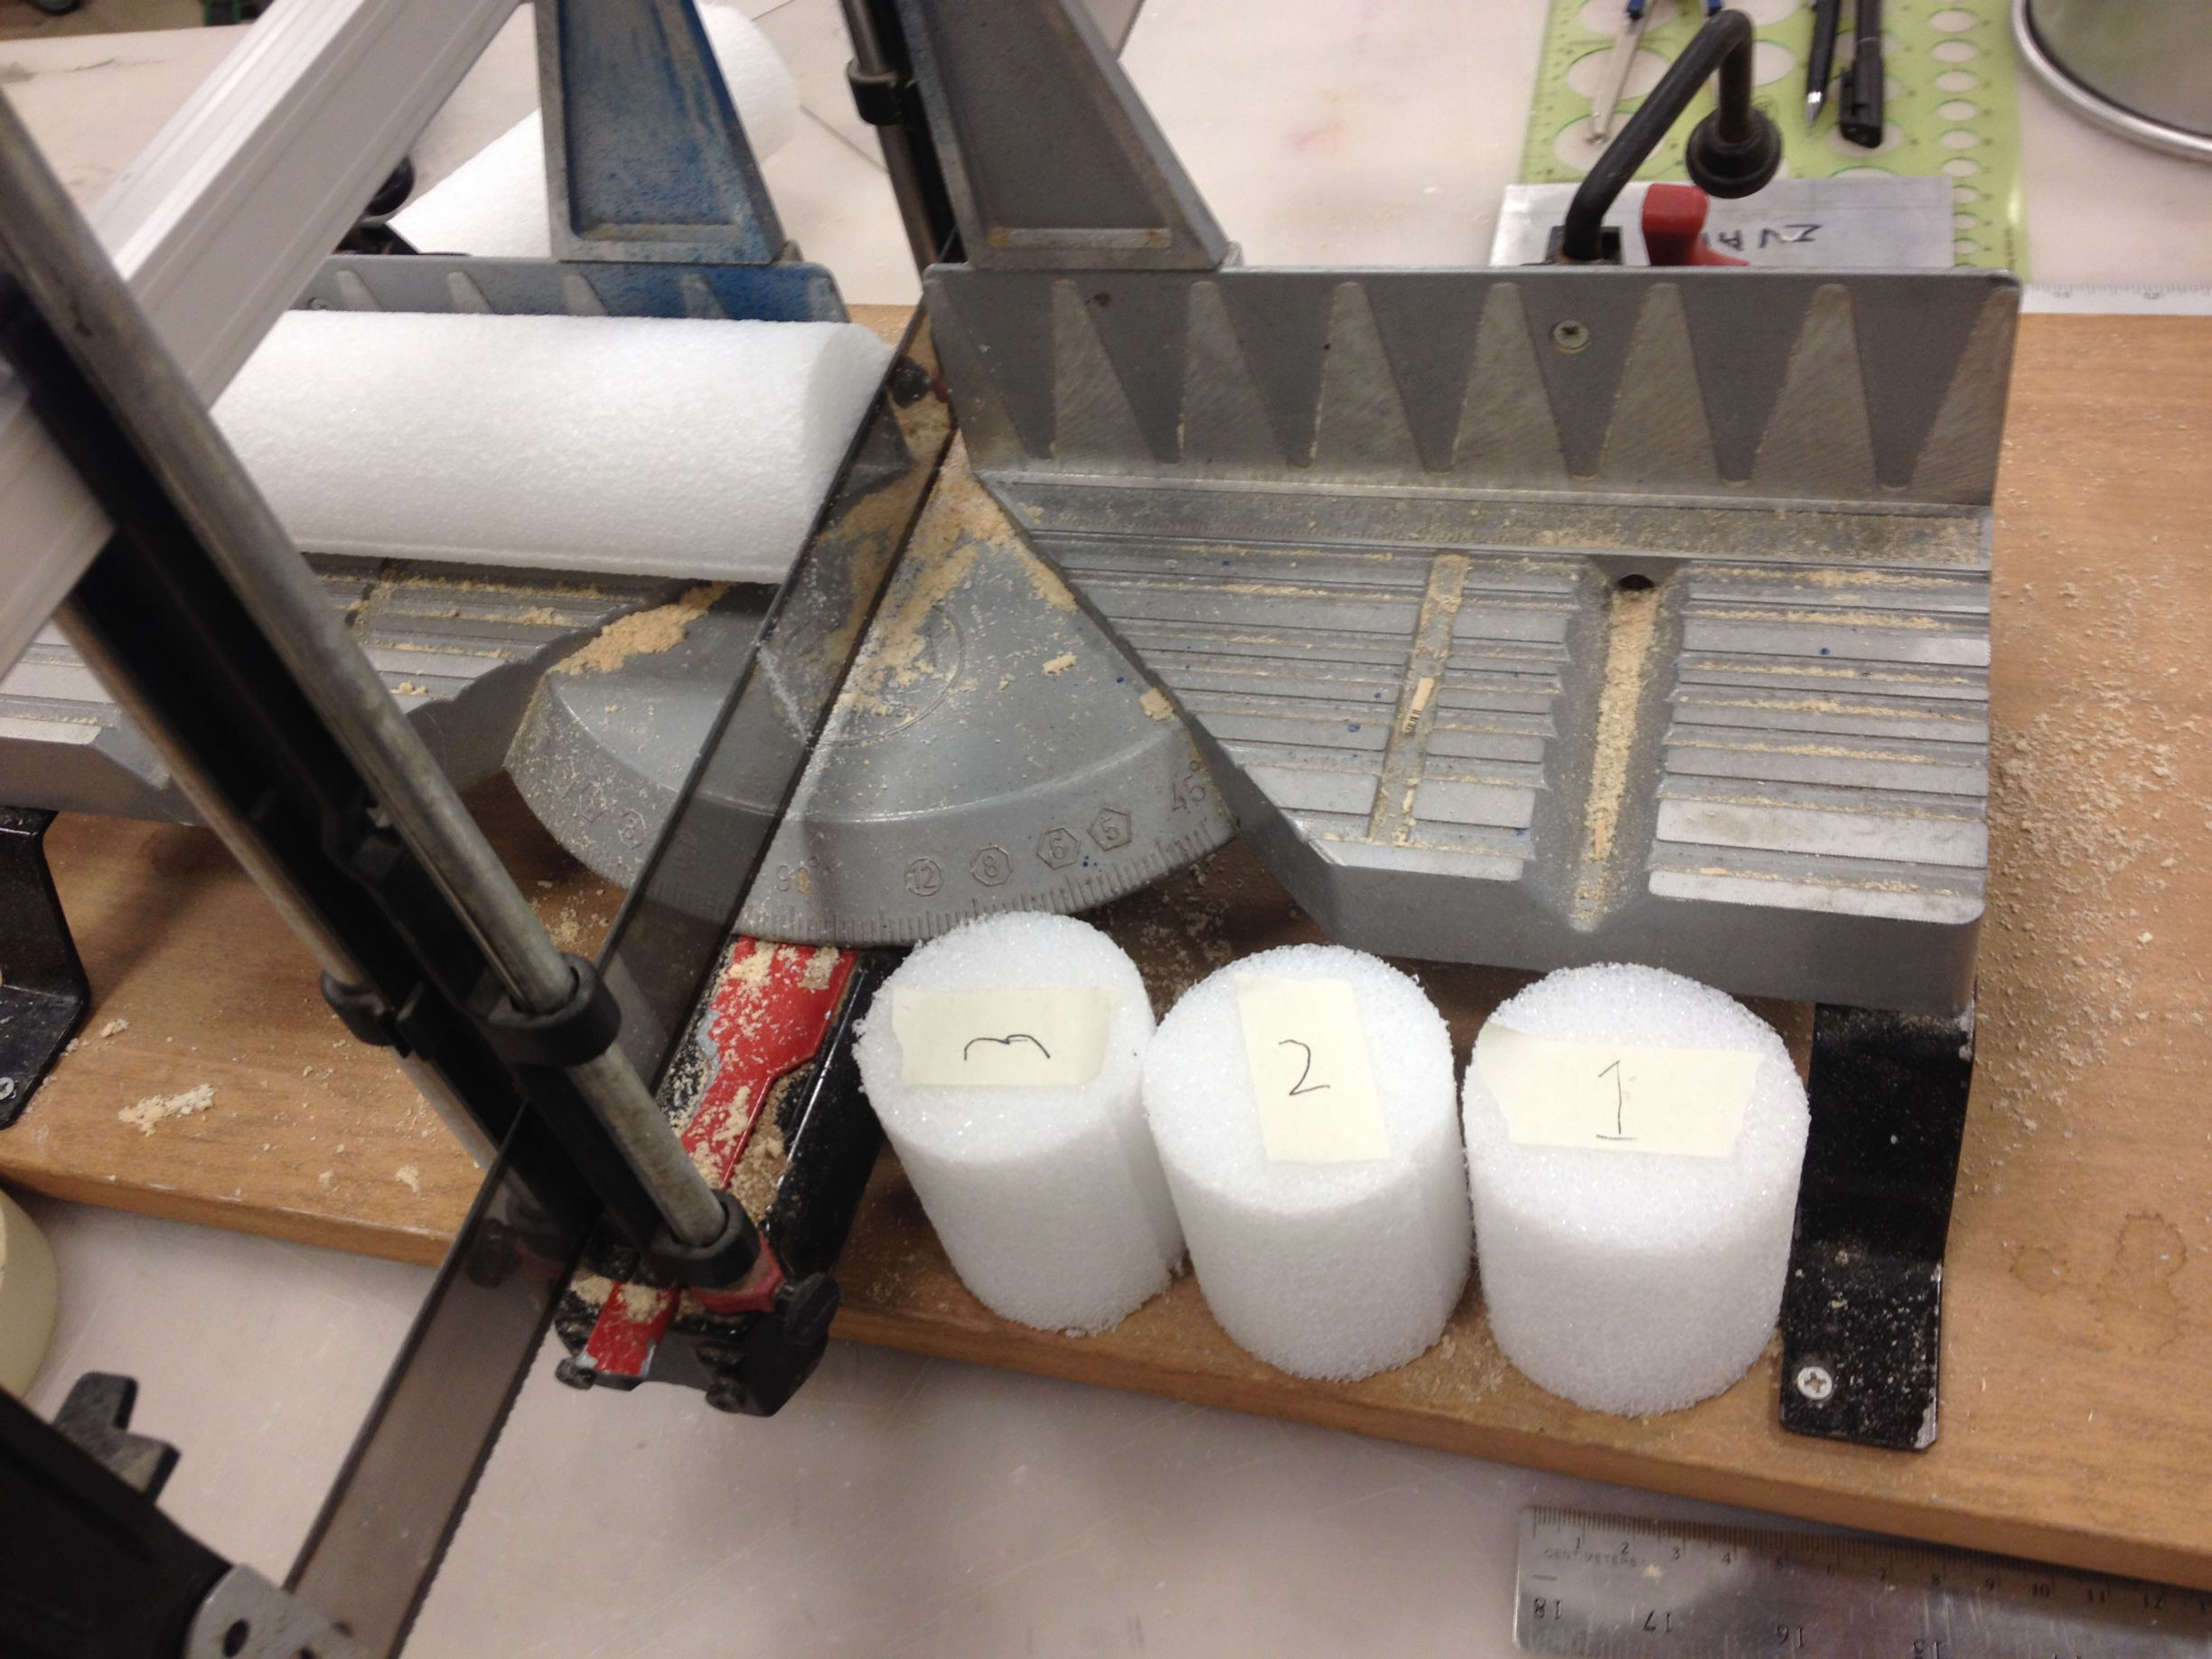
\includegraphics[scale=0.15]{feed/01.jpeg}
\end{center}

The Styrofoam was measured from multiple sides to determine the center. The rod we have ranges from 2 5/16" to 2 1/2" in diameter.

We used a drill press with a 1/4" bit. The Styrofoam was held by a vice on the drilling table. (The Styrofoam is a bit messy so we put down a rag under the vice) 

\begin{center}
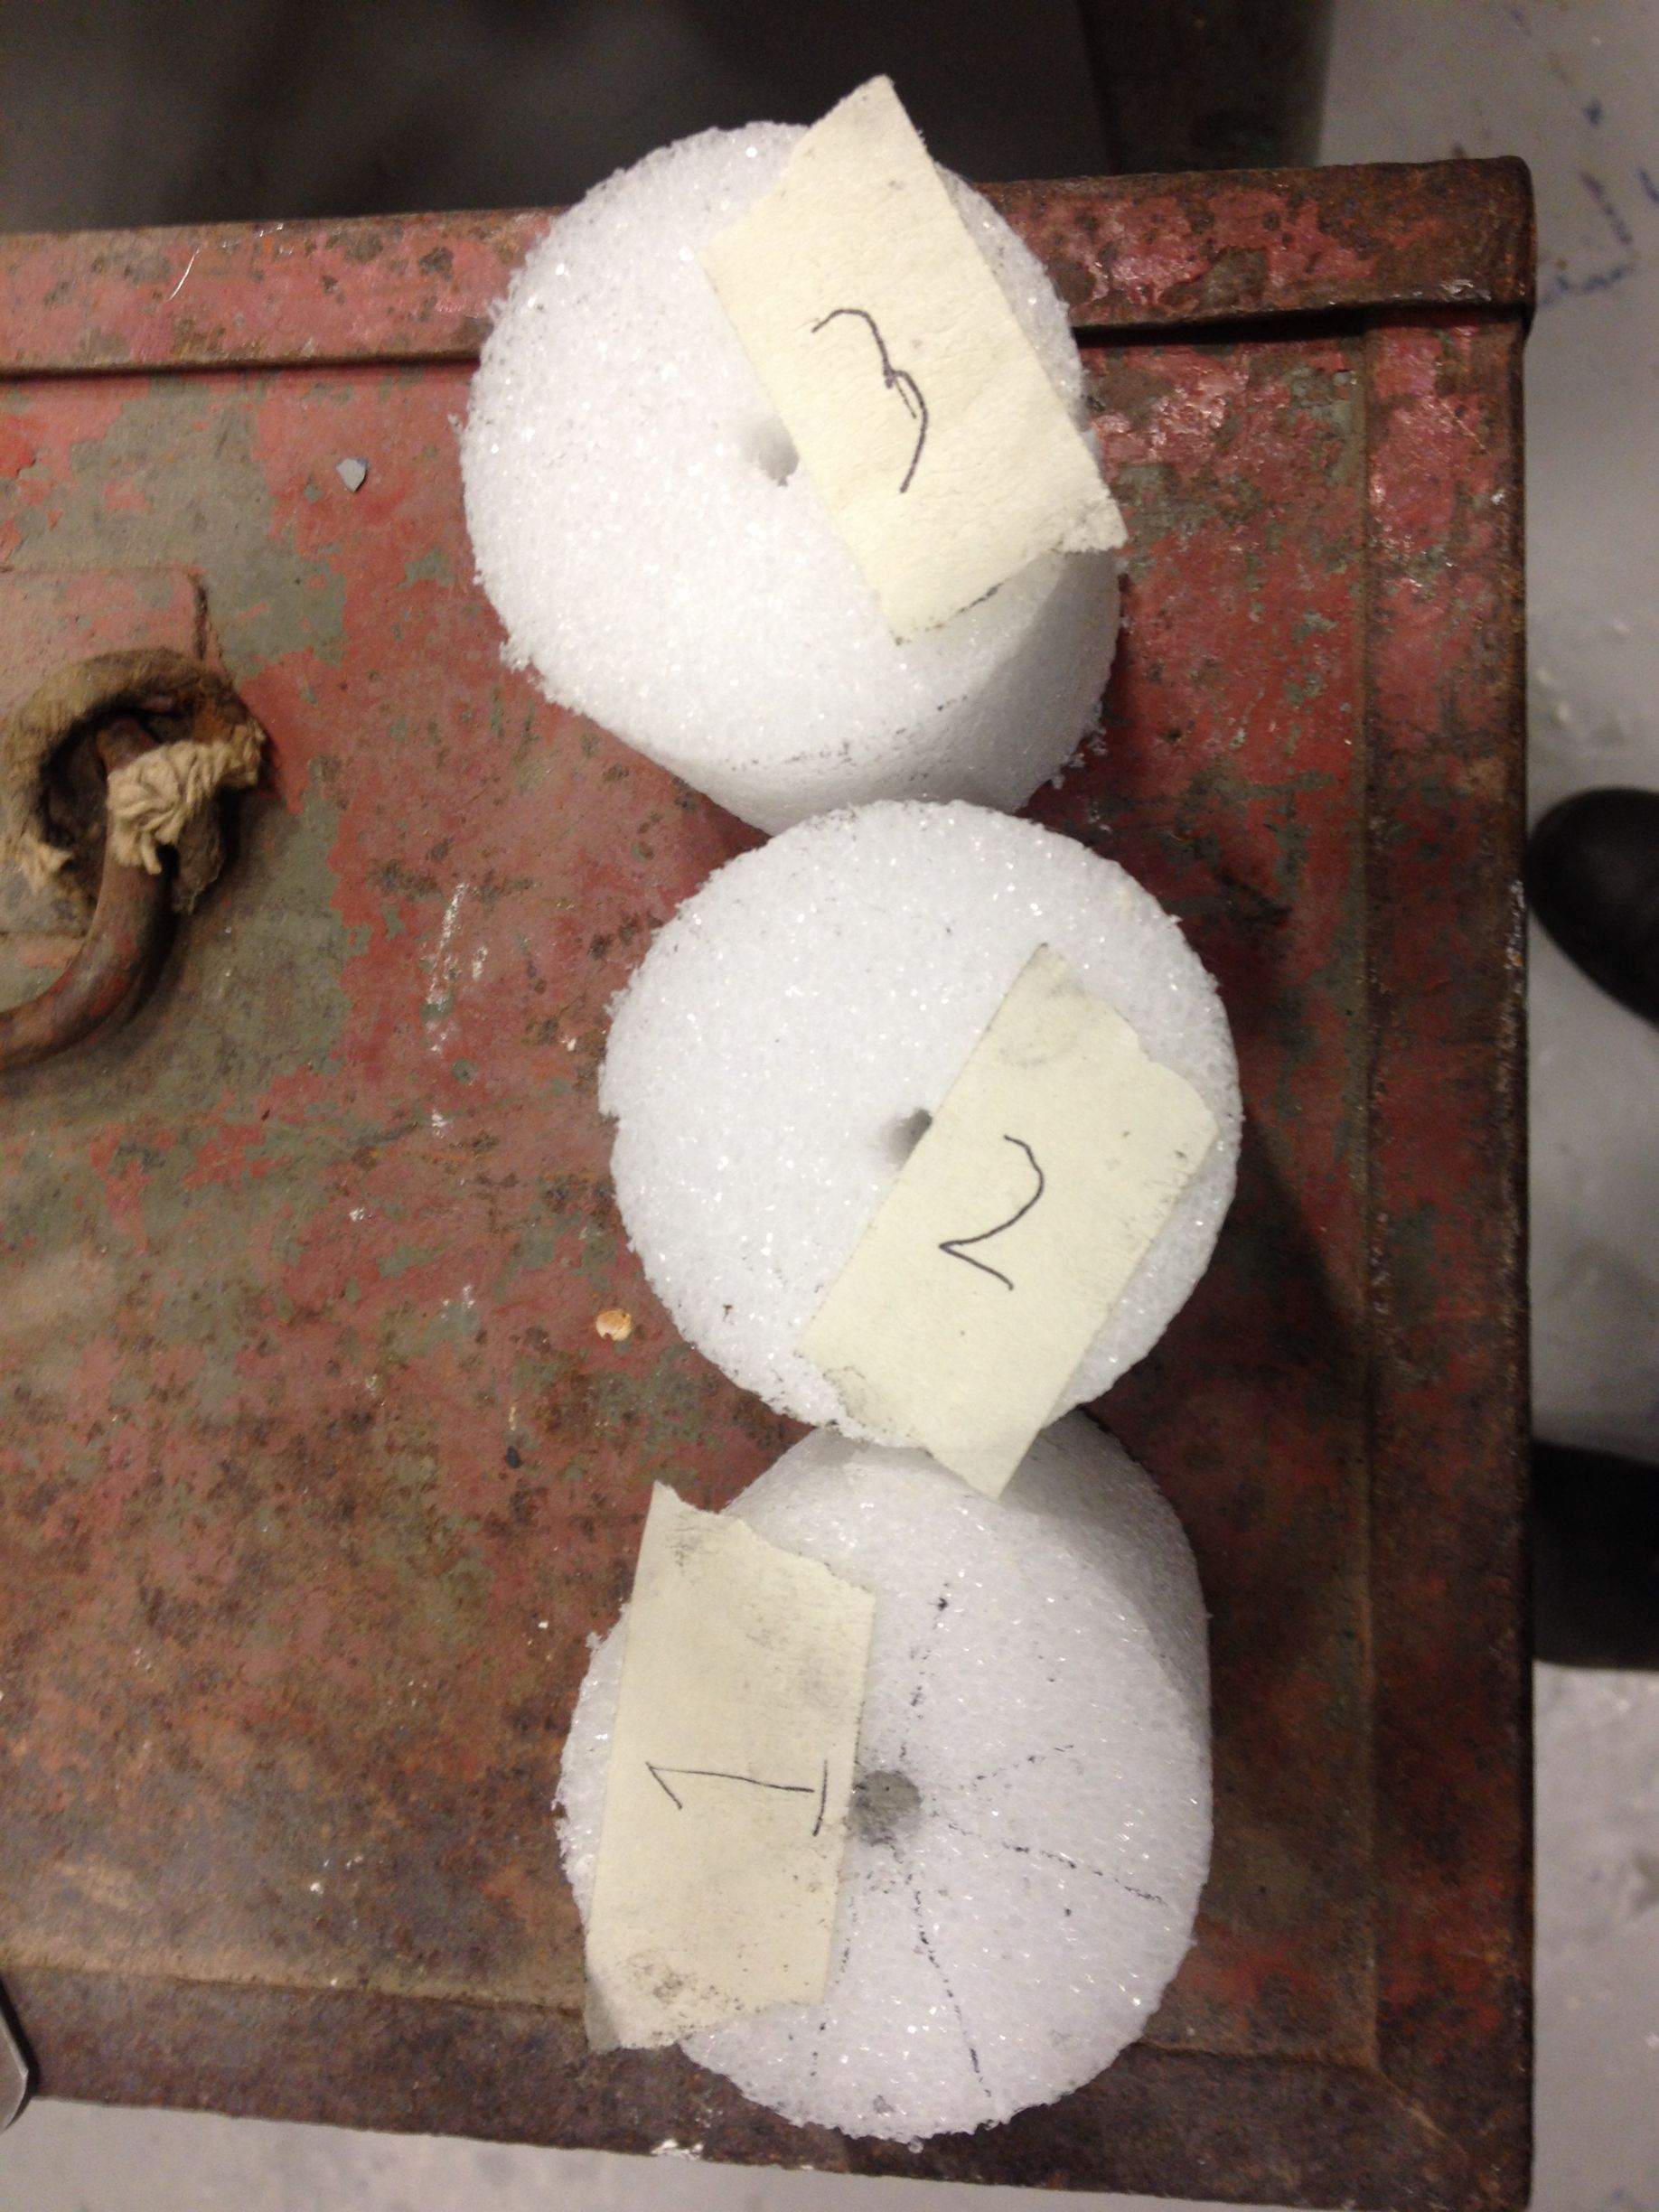
\includegraphics[scale=0.09]{feed/02.jpeg}
\end{center}

Note: we made three rods to provide room for error in the application and soldering of the copper tape later.

\subsubsection{Drilling Aluminum LNA Base Plate}

We put the plate in a vice which we secured on the drill press table with some heavy steel blocks.

\begin{center}
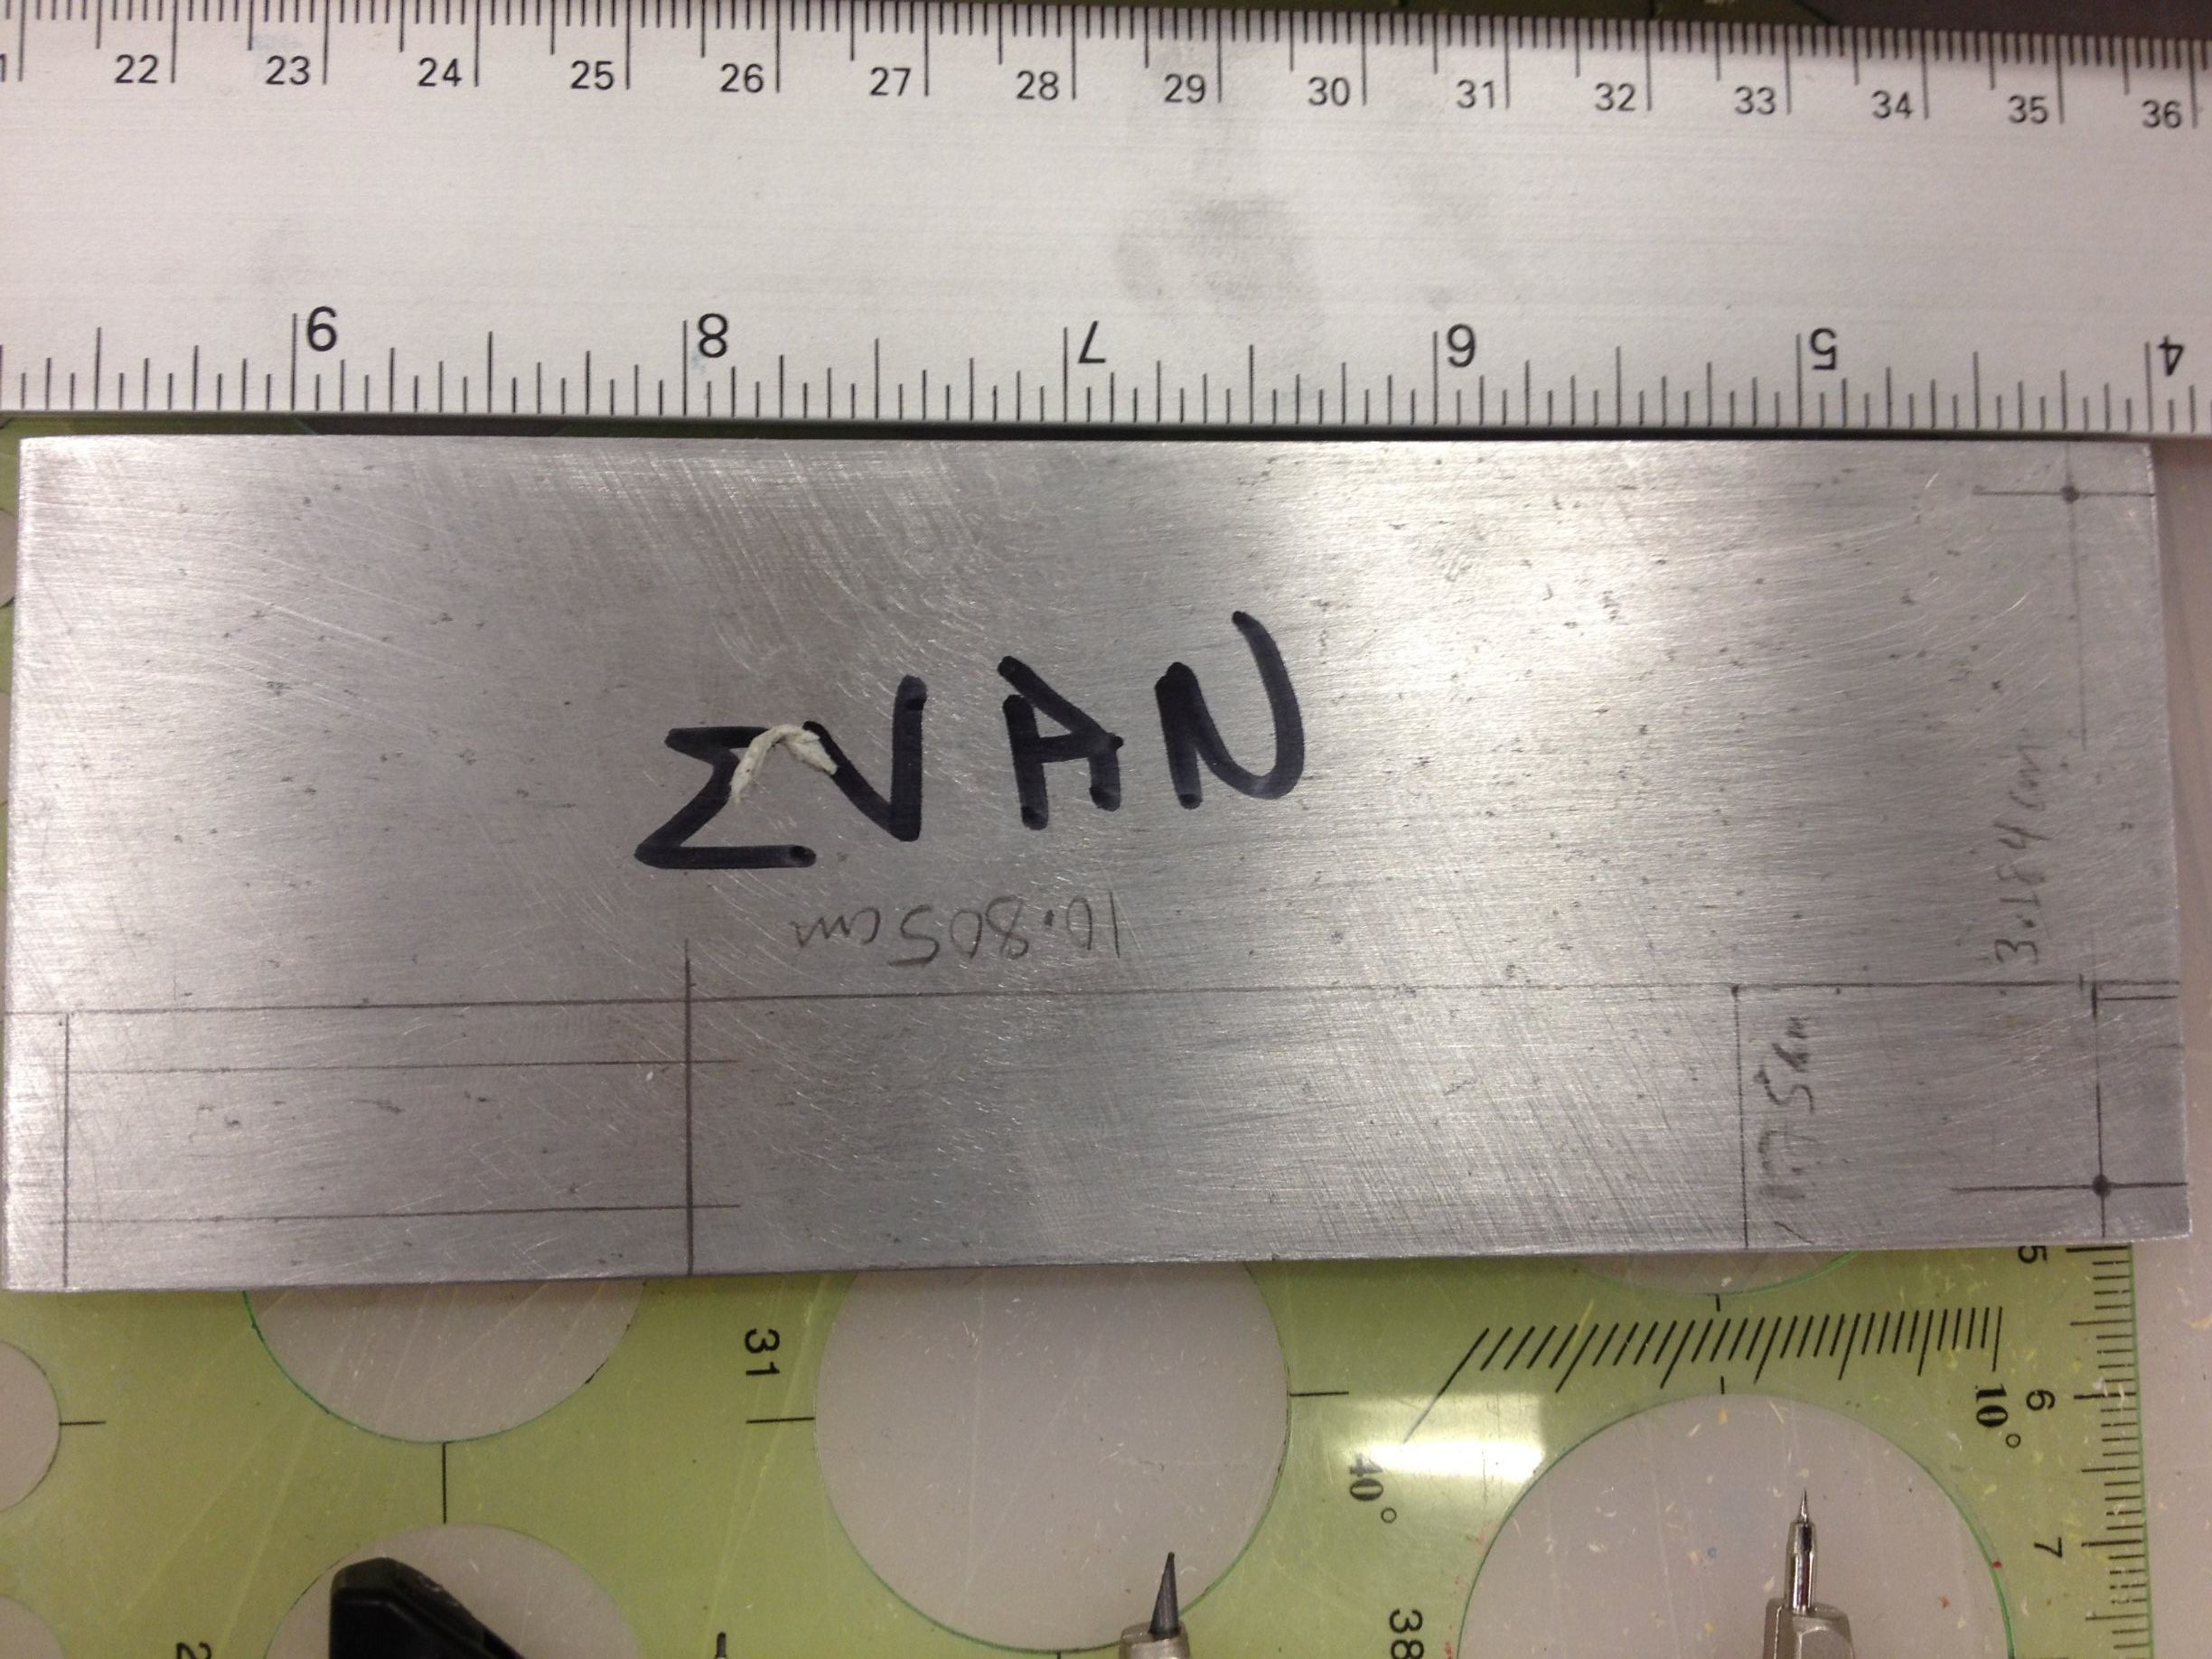
\includegraphics[scale=0.12]{feed/03.jpeg}
\end{center}

\subsubsection{Drilling Aluminum Cake Pan}

We made the measurements of the cake pan working out from the center which we found by transecting the circle and then making perpendicular rays from the center of each line cutting across the arc. This proved to be adequately precise. 

\begin{center}
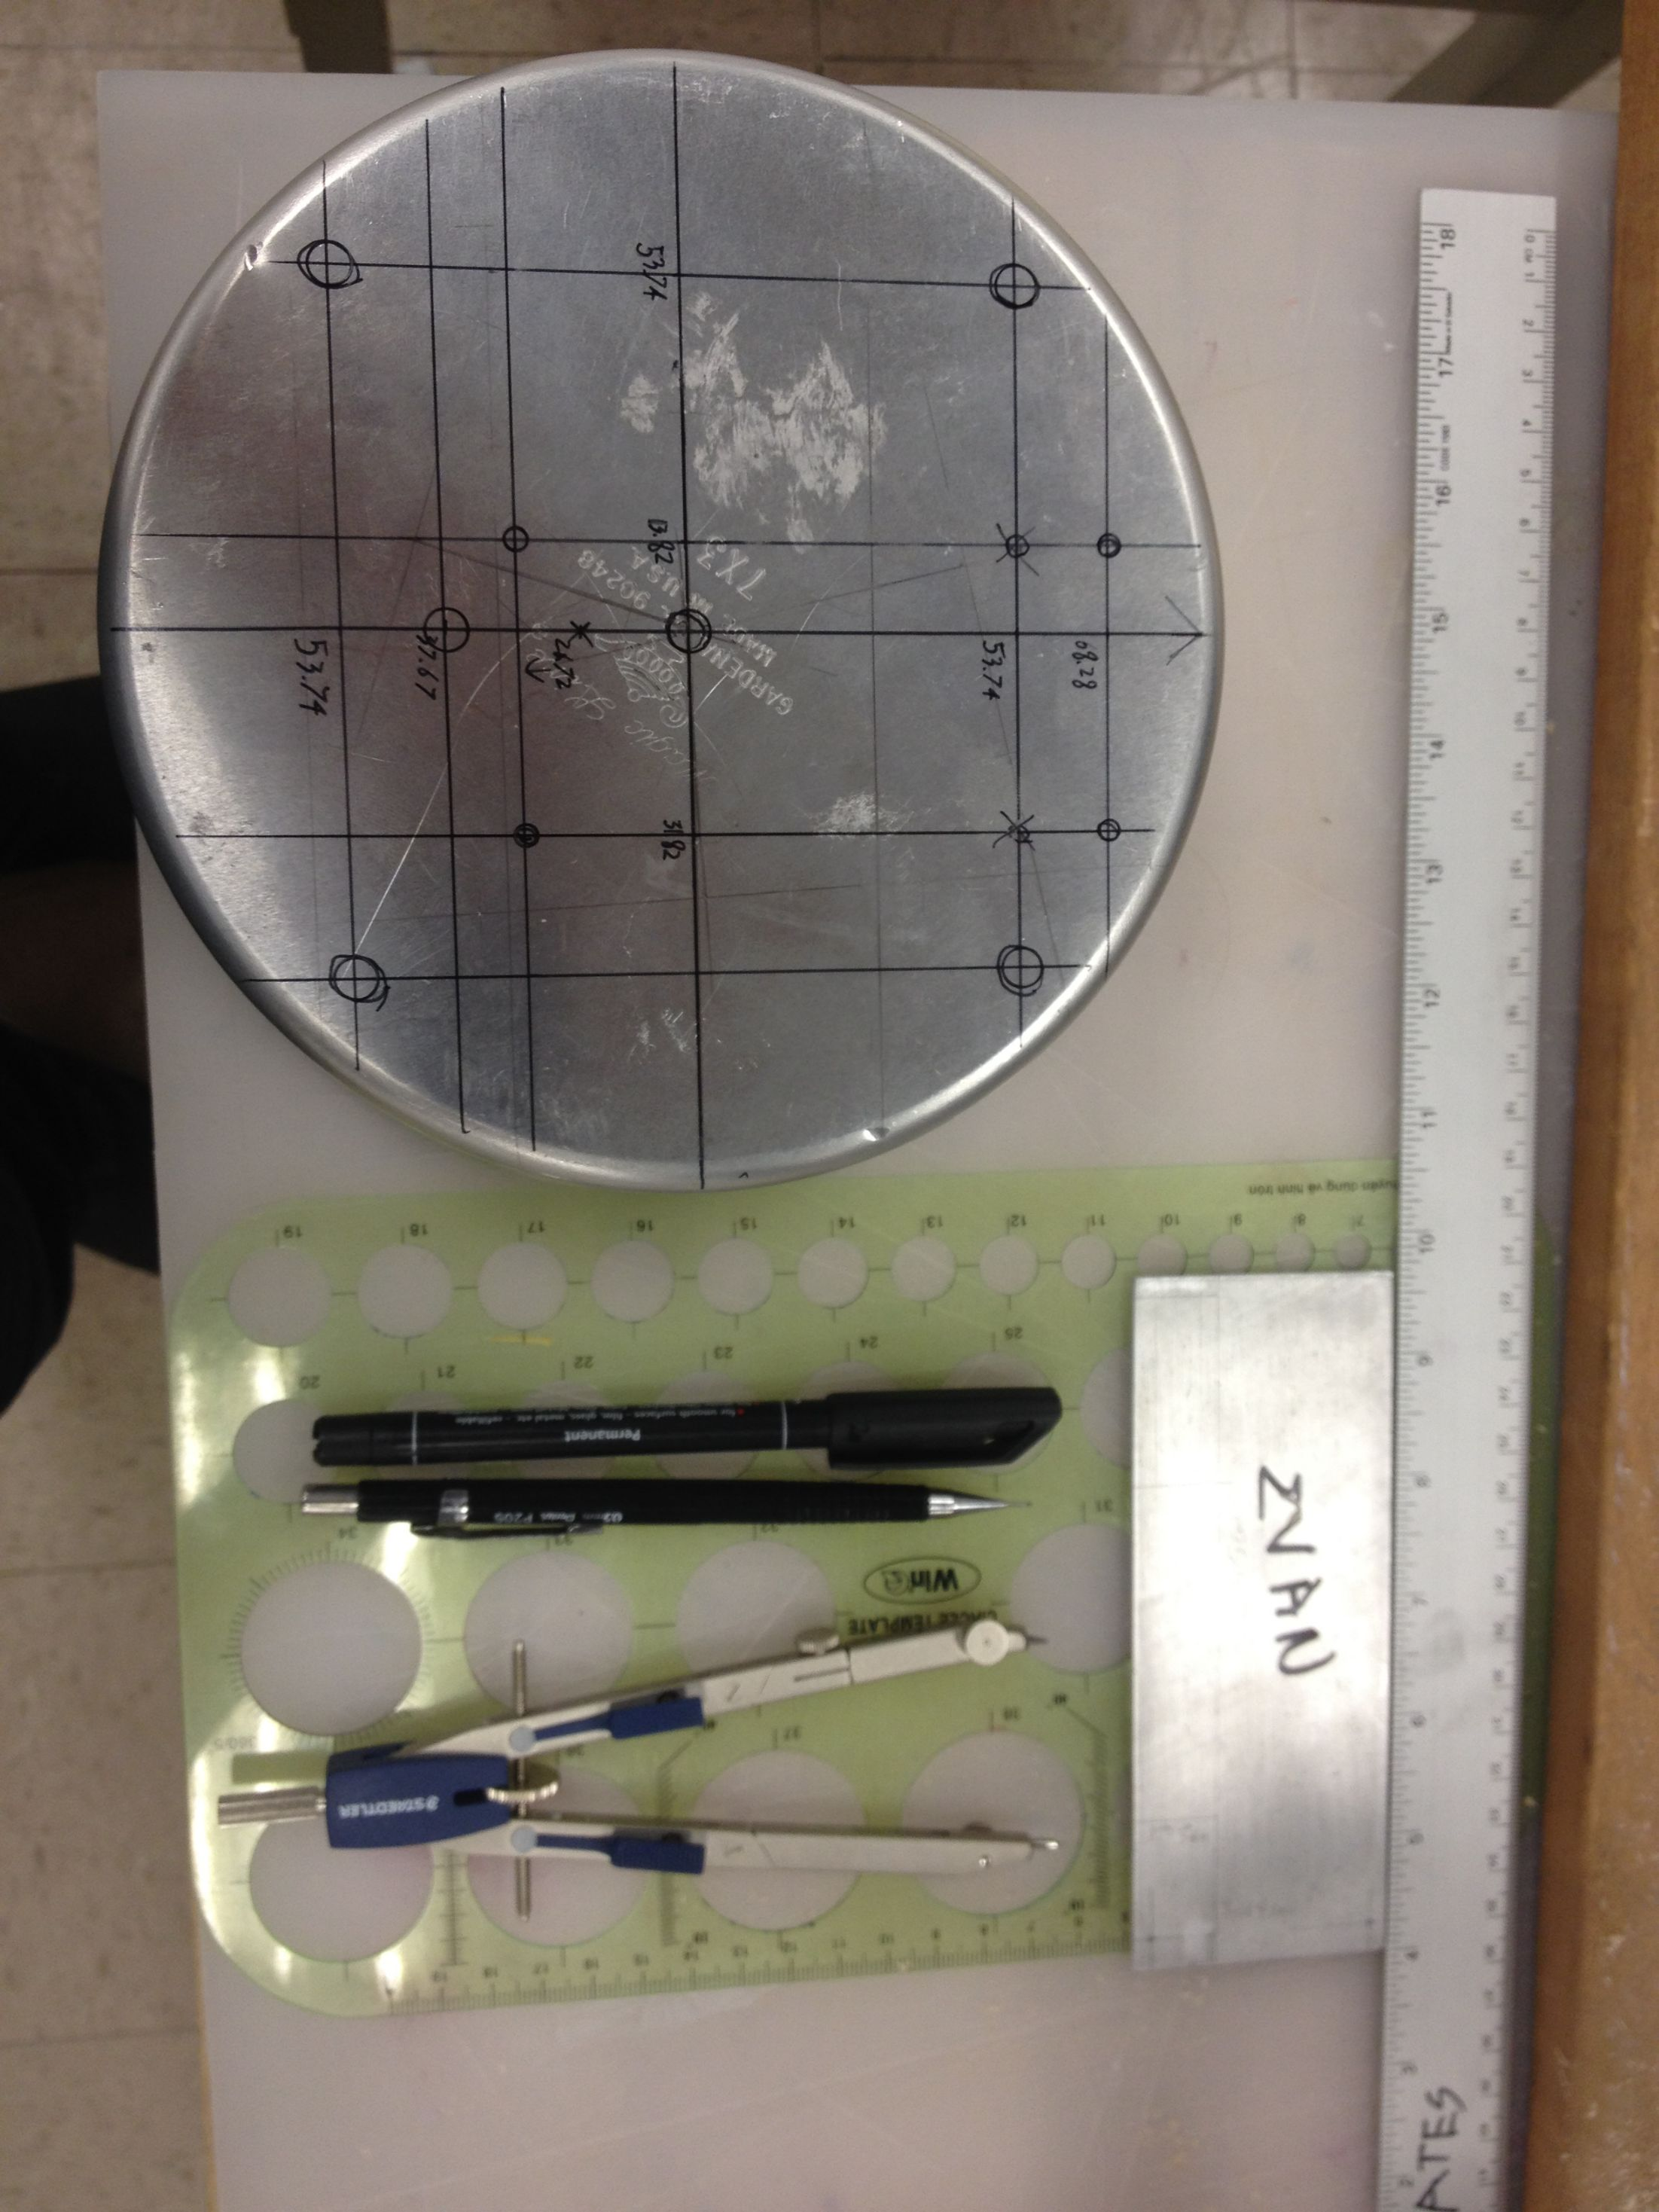
\includegraphics[scale=0.11]{feed/04.jpeg}
\end{center}

The cake pan was more of a challenge to drill than the base plate as it was tricky to secure to the drill press table so we could make accurate holes. We ended up putting a 4" piece of angle iron on the pan and then clamping that down to the edges of the table. 

\begin{center}
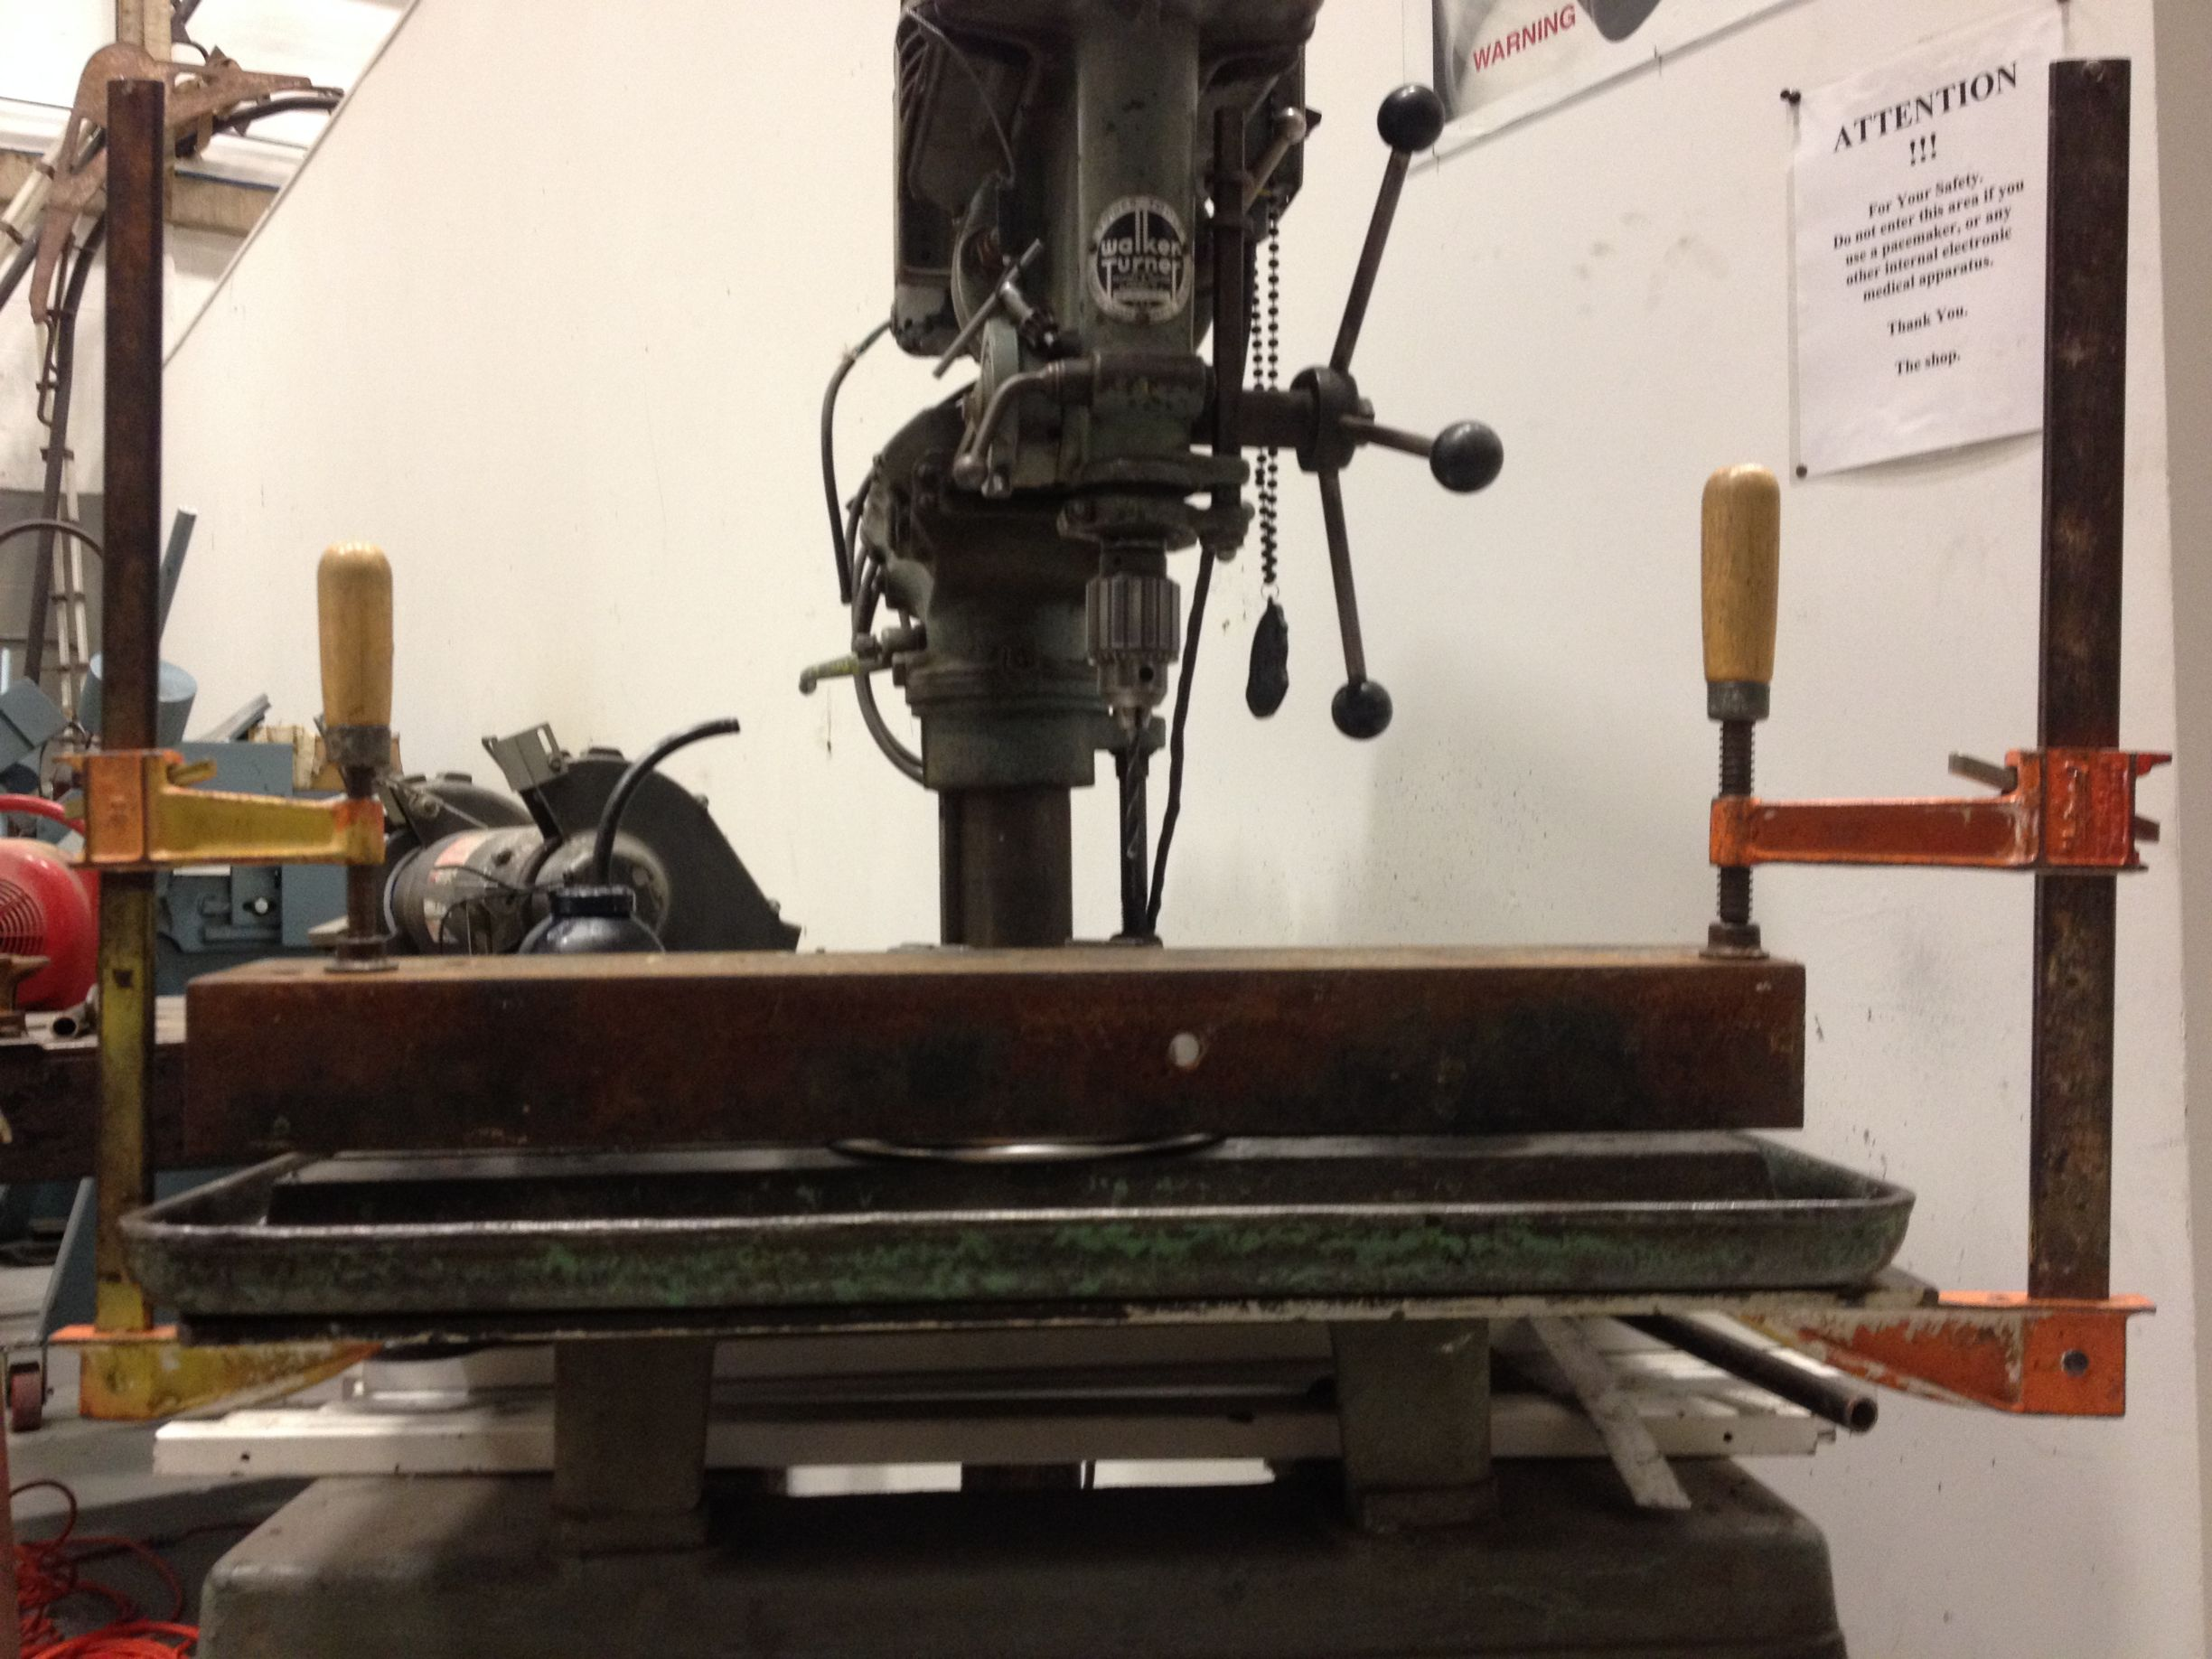
\includegraphics[scale=0.15]{feed/05.jpeg}
\end{center}

Finished drilling

\begin{center}
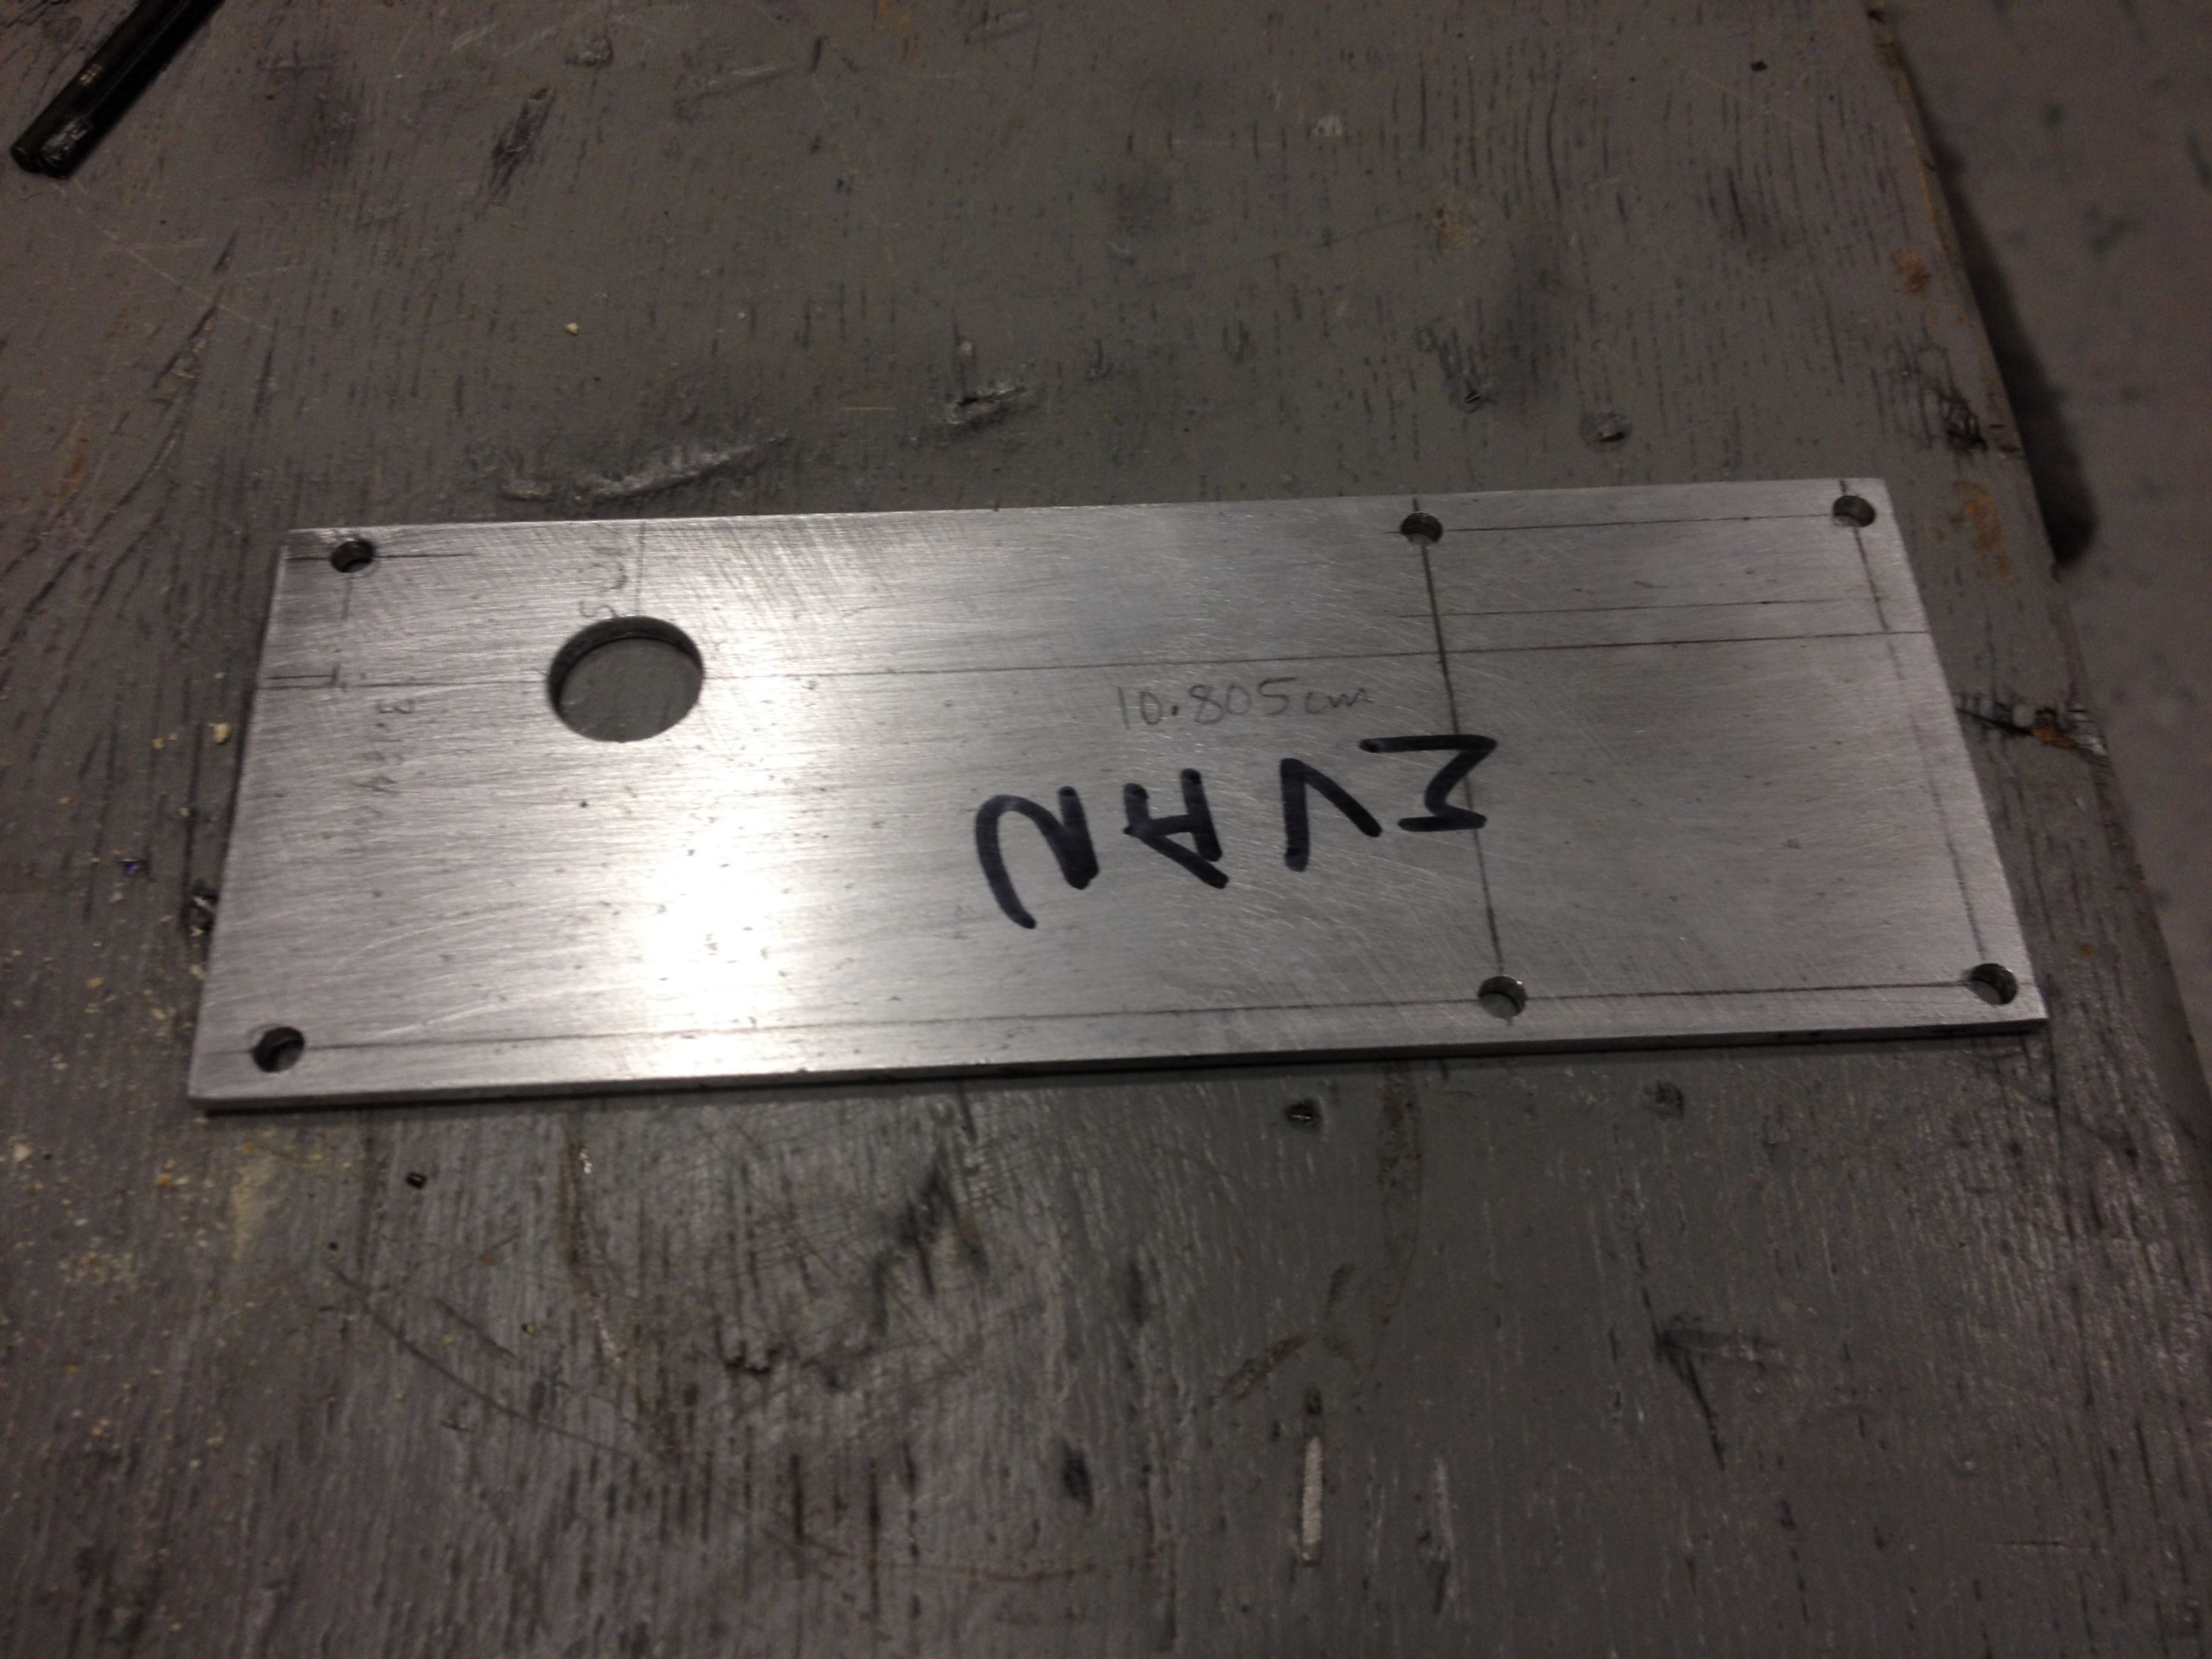
\includegraphics[scale=0.10]{feed/06.jpeg}
\end{center}

\begin{center}
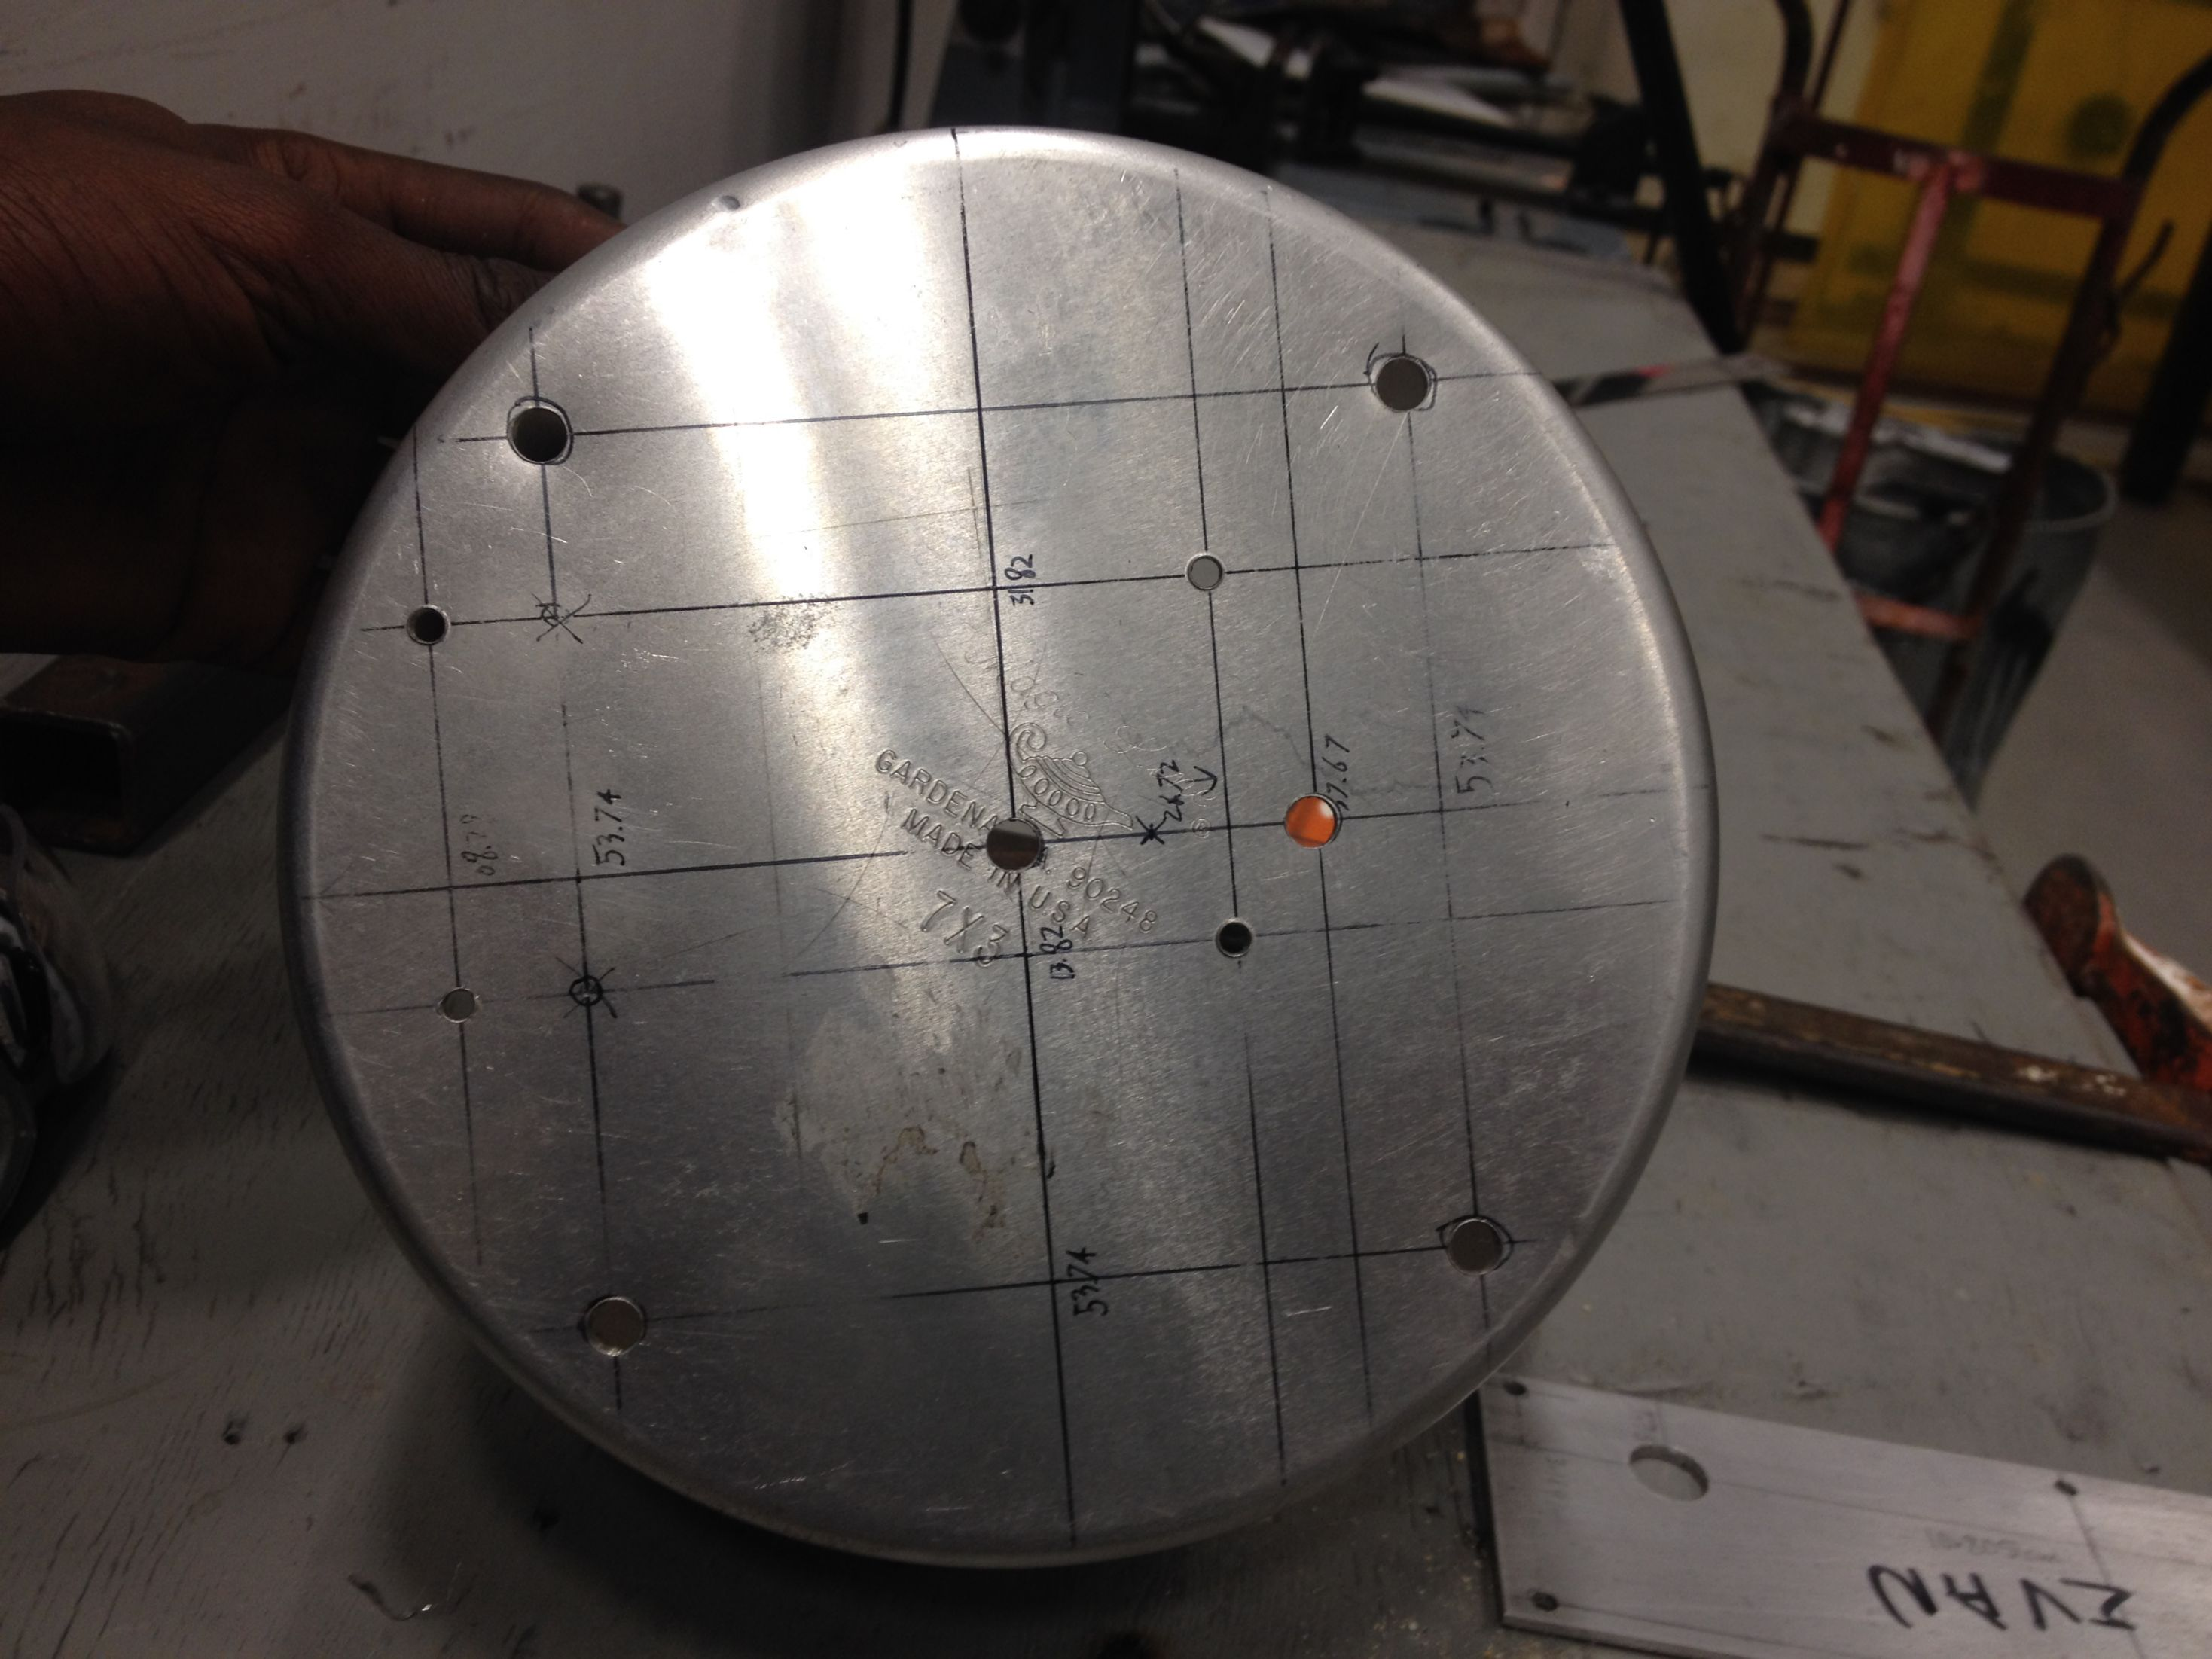
\includegraphics[scale=0.11]{feed/07.jpeg}
\end{center}

\subsubsection{Minor concerns}
The drilling instructions are precise to a 100th of a millimeter. We did the drilling with a drill press, not a CNC machine, so I would say our precision was closer to a 10th of a millimeter.

Also, the cake pan is really not a precisely made object, it is certainly not as precise as the schematics given by MIT. I think that indicates that our slight reduction in precision will be fine.

The cake pan is made of what seems to be a softer aluminum than the LNA base plate. This made the metal not cut cleanly on the inside of the pan (the bit went through the outside first). The holes are the correct dimensions but there is some extra material around the holes. I have tried to clean it up with an x-acto knife and been relatively successful. I think the metal is so soft that these small bits of extra material will be squished when we insert the hardware, making their effect negligible. 

\begin{center}
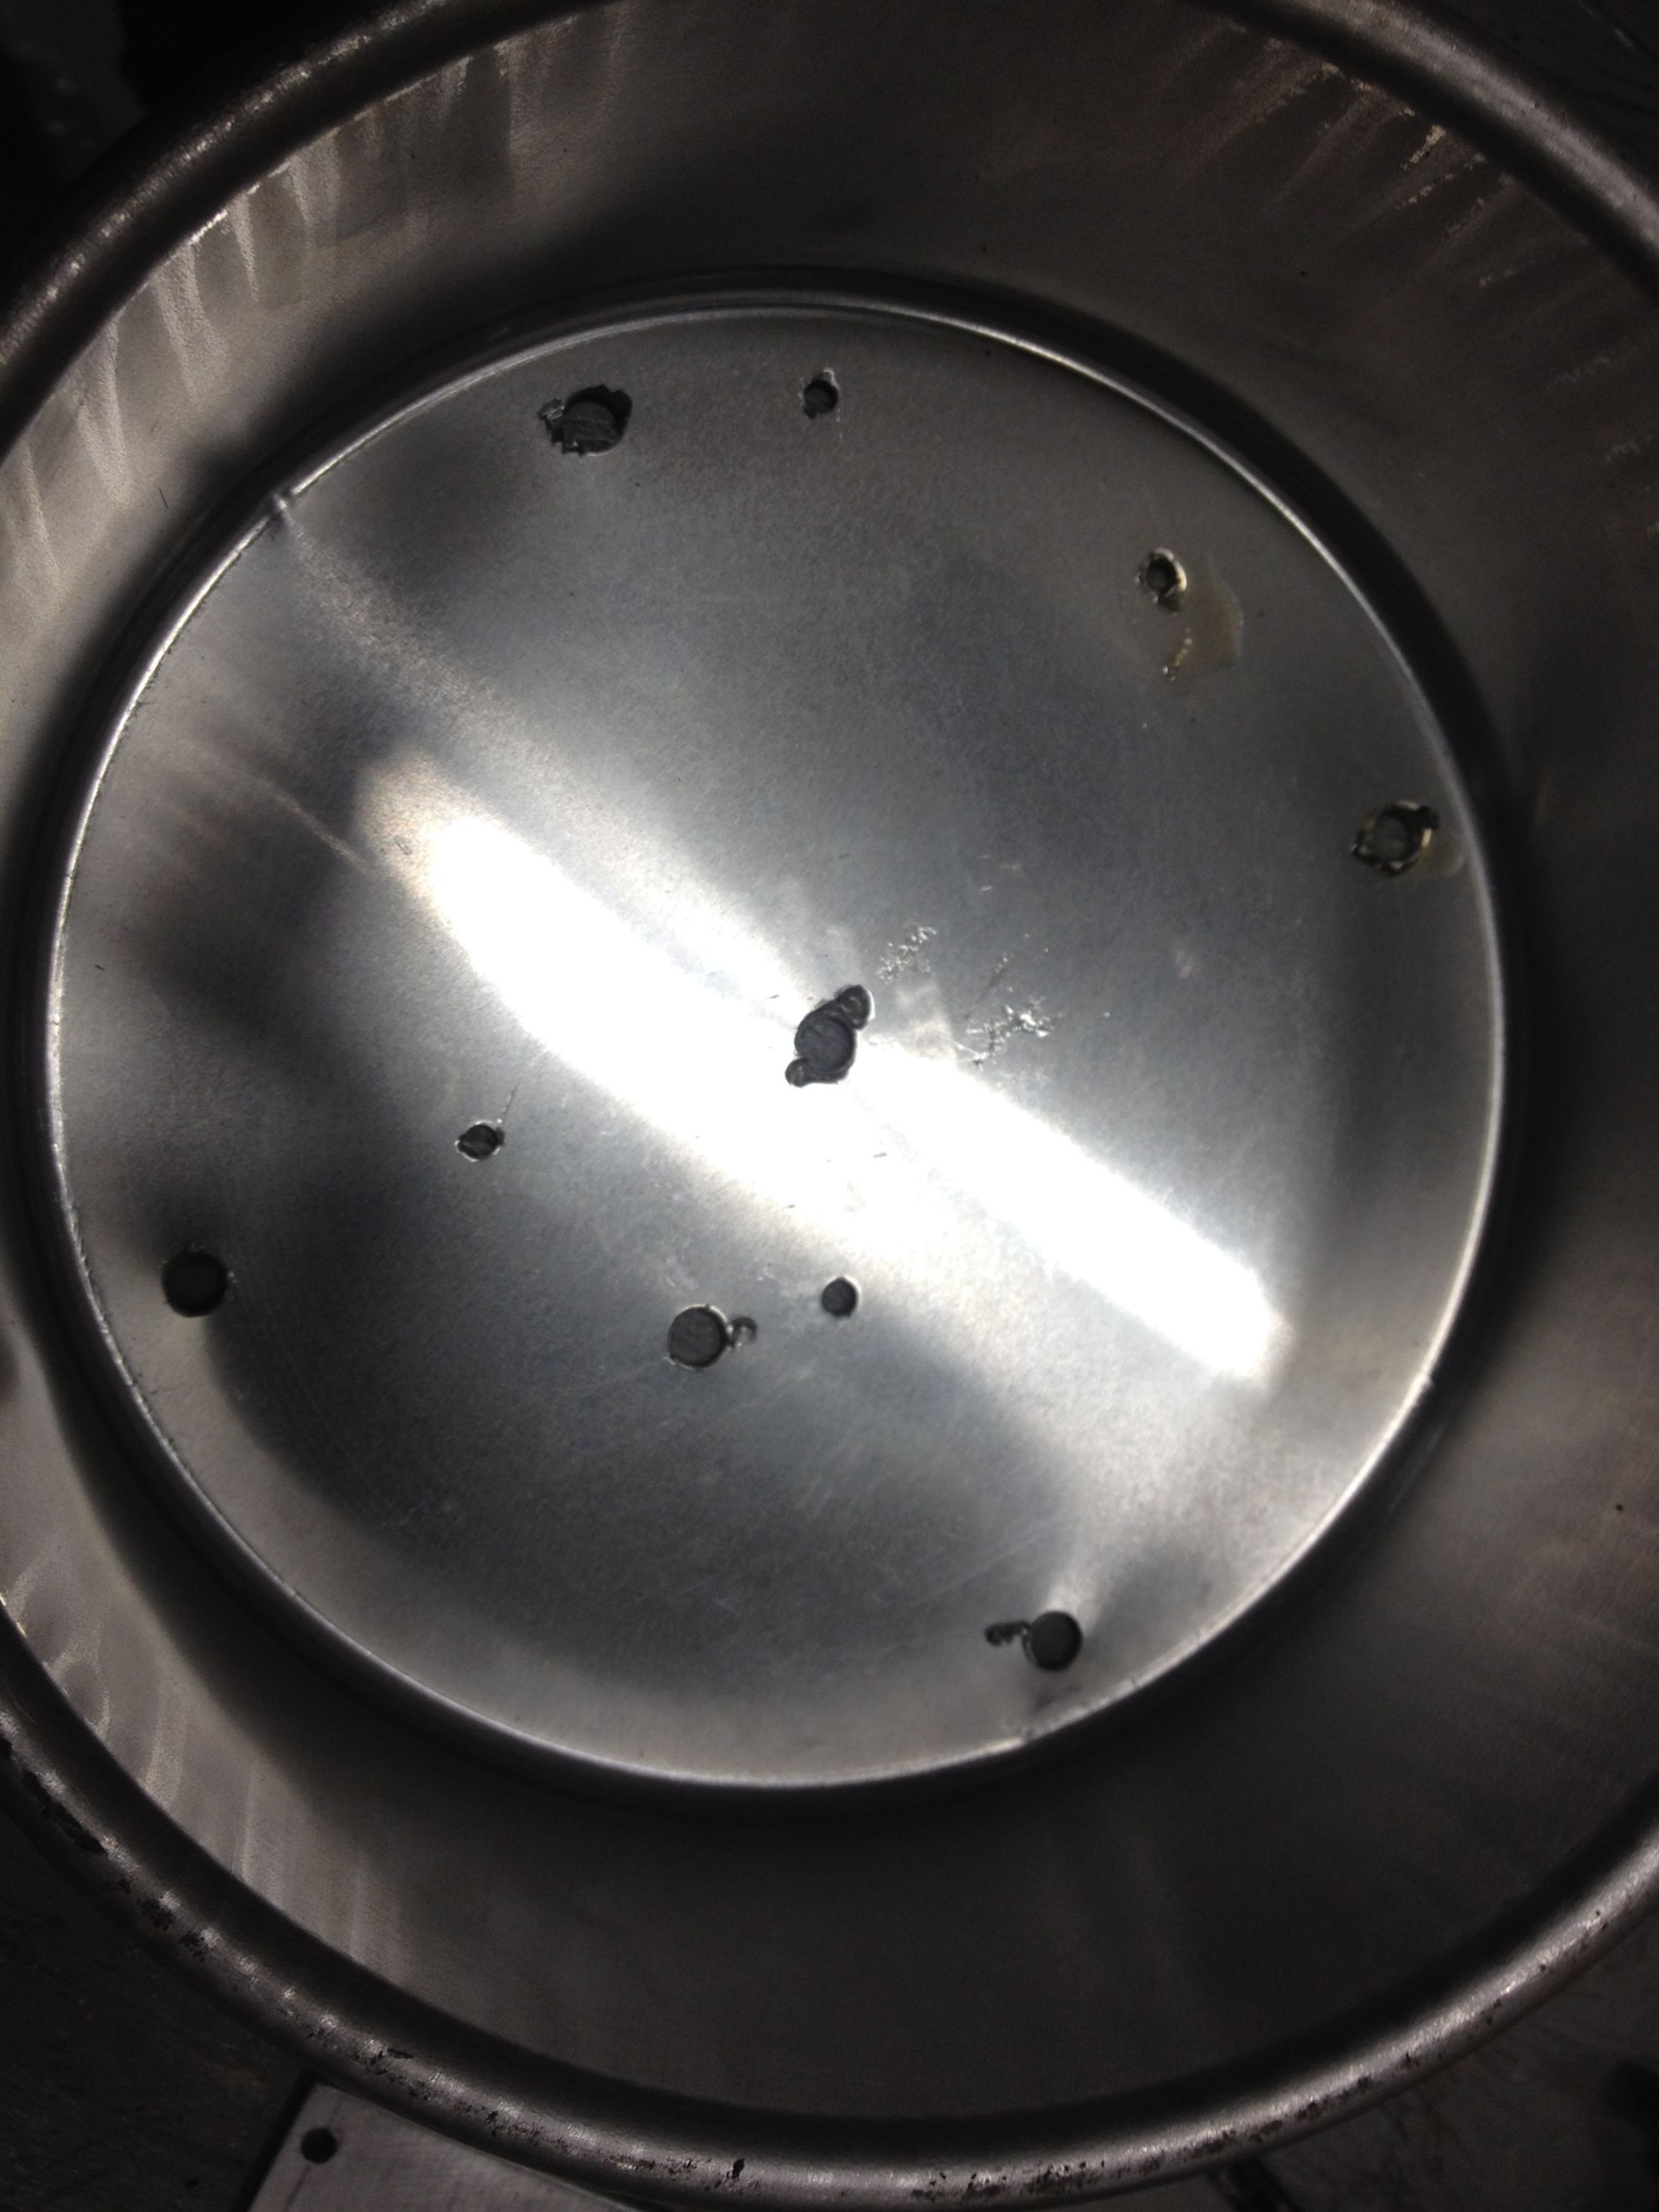
\includegraphics[scale=0.12]{feed/08.jpeg}
\end{center}

\subsubsection{Making helical antenna}
We cut out strips of copper tape with an X-acto knife and a straight edge. 

\begin{center}
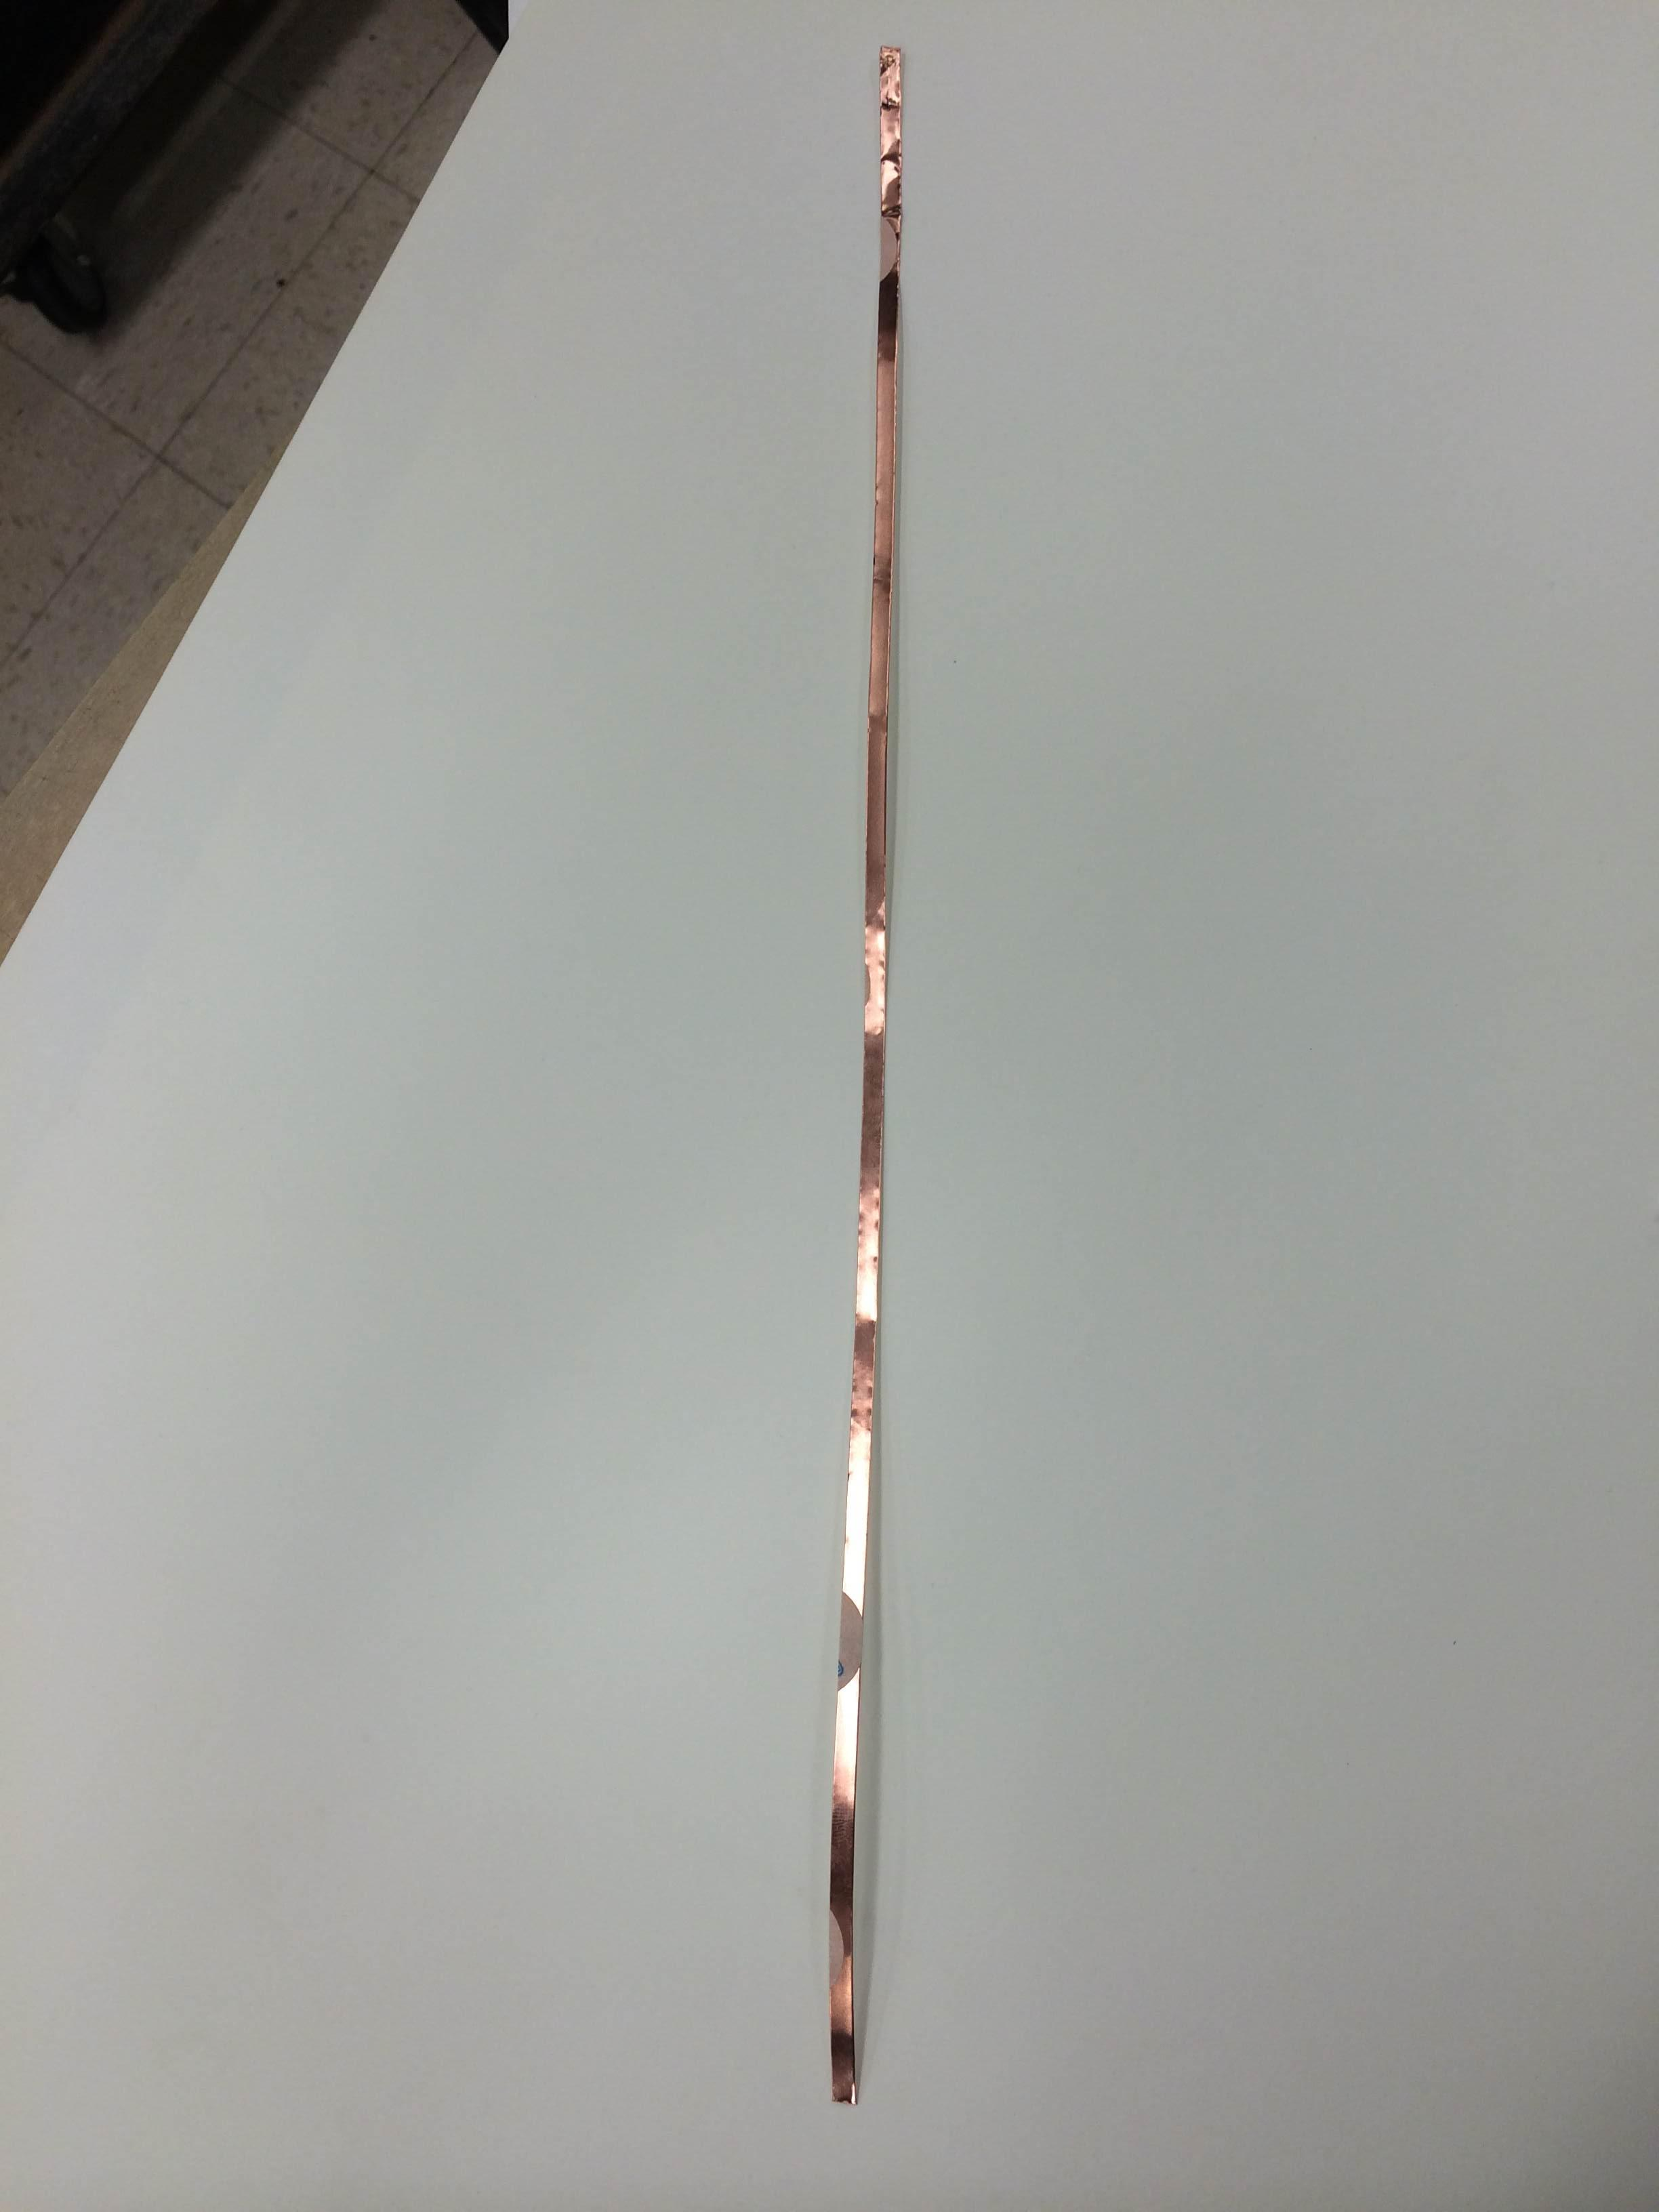
\includegraphics[scale=0.10]{feed/09.jpeg}
\end{center}

Then we measured marked the styrofoam rod at even intervals as specified by the manual to get a consistent helix with the tape. 

\begin{center}
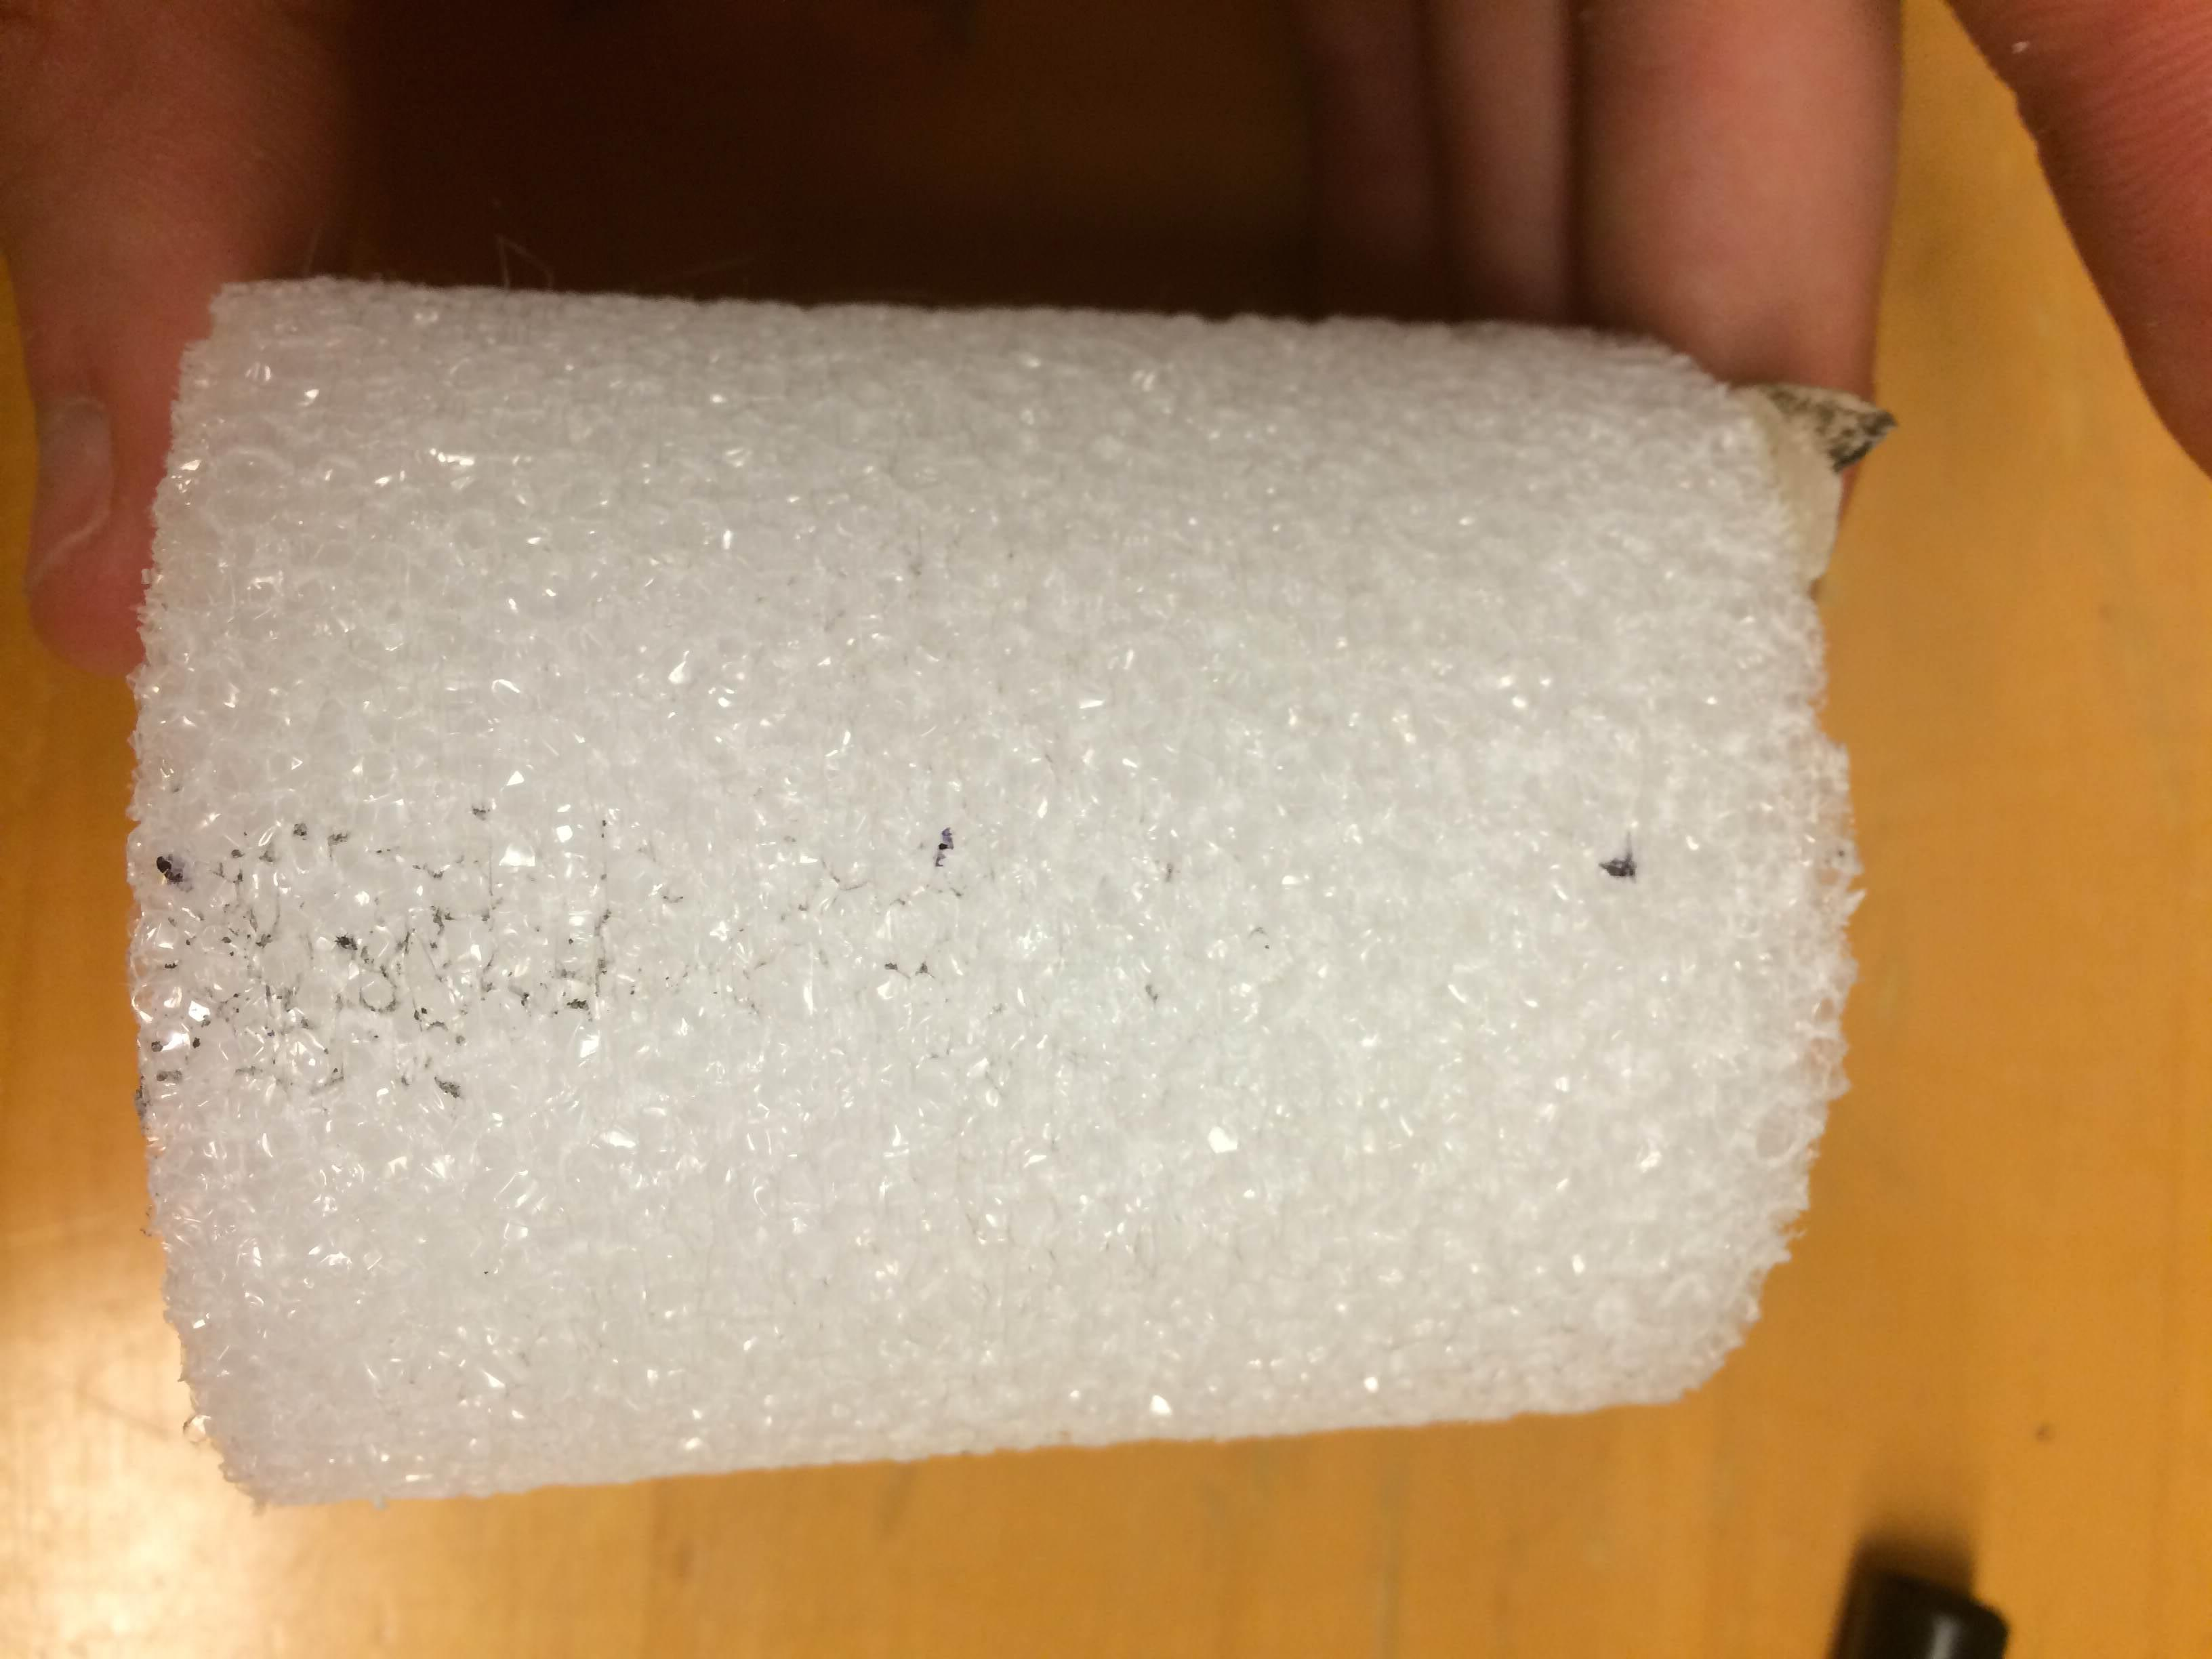
\includegraphics[scale=0.08]{feed/10.jpeg}
\end{center}

\begin{center}
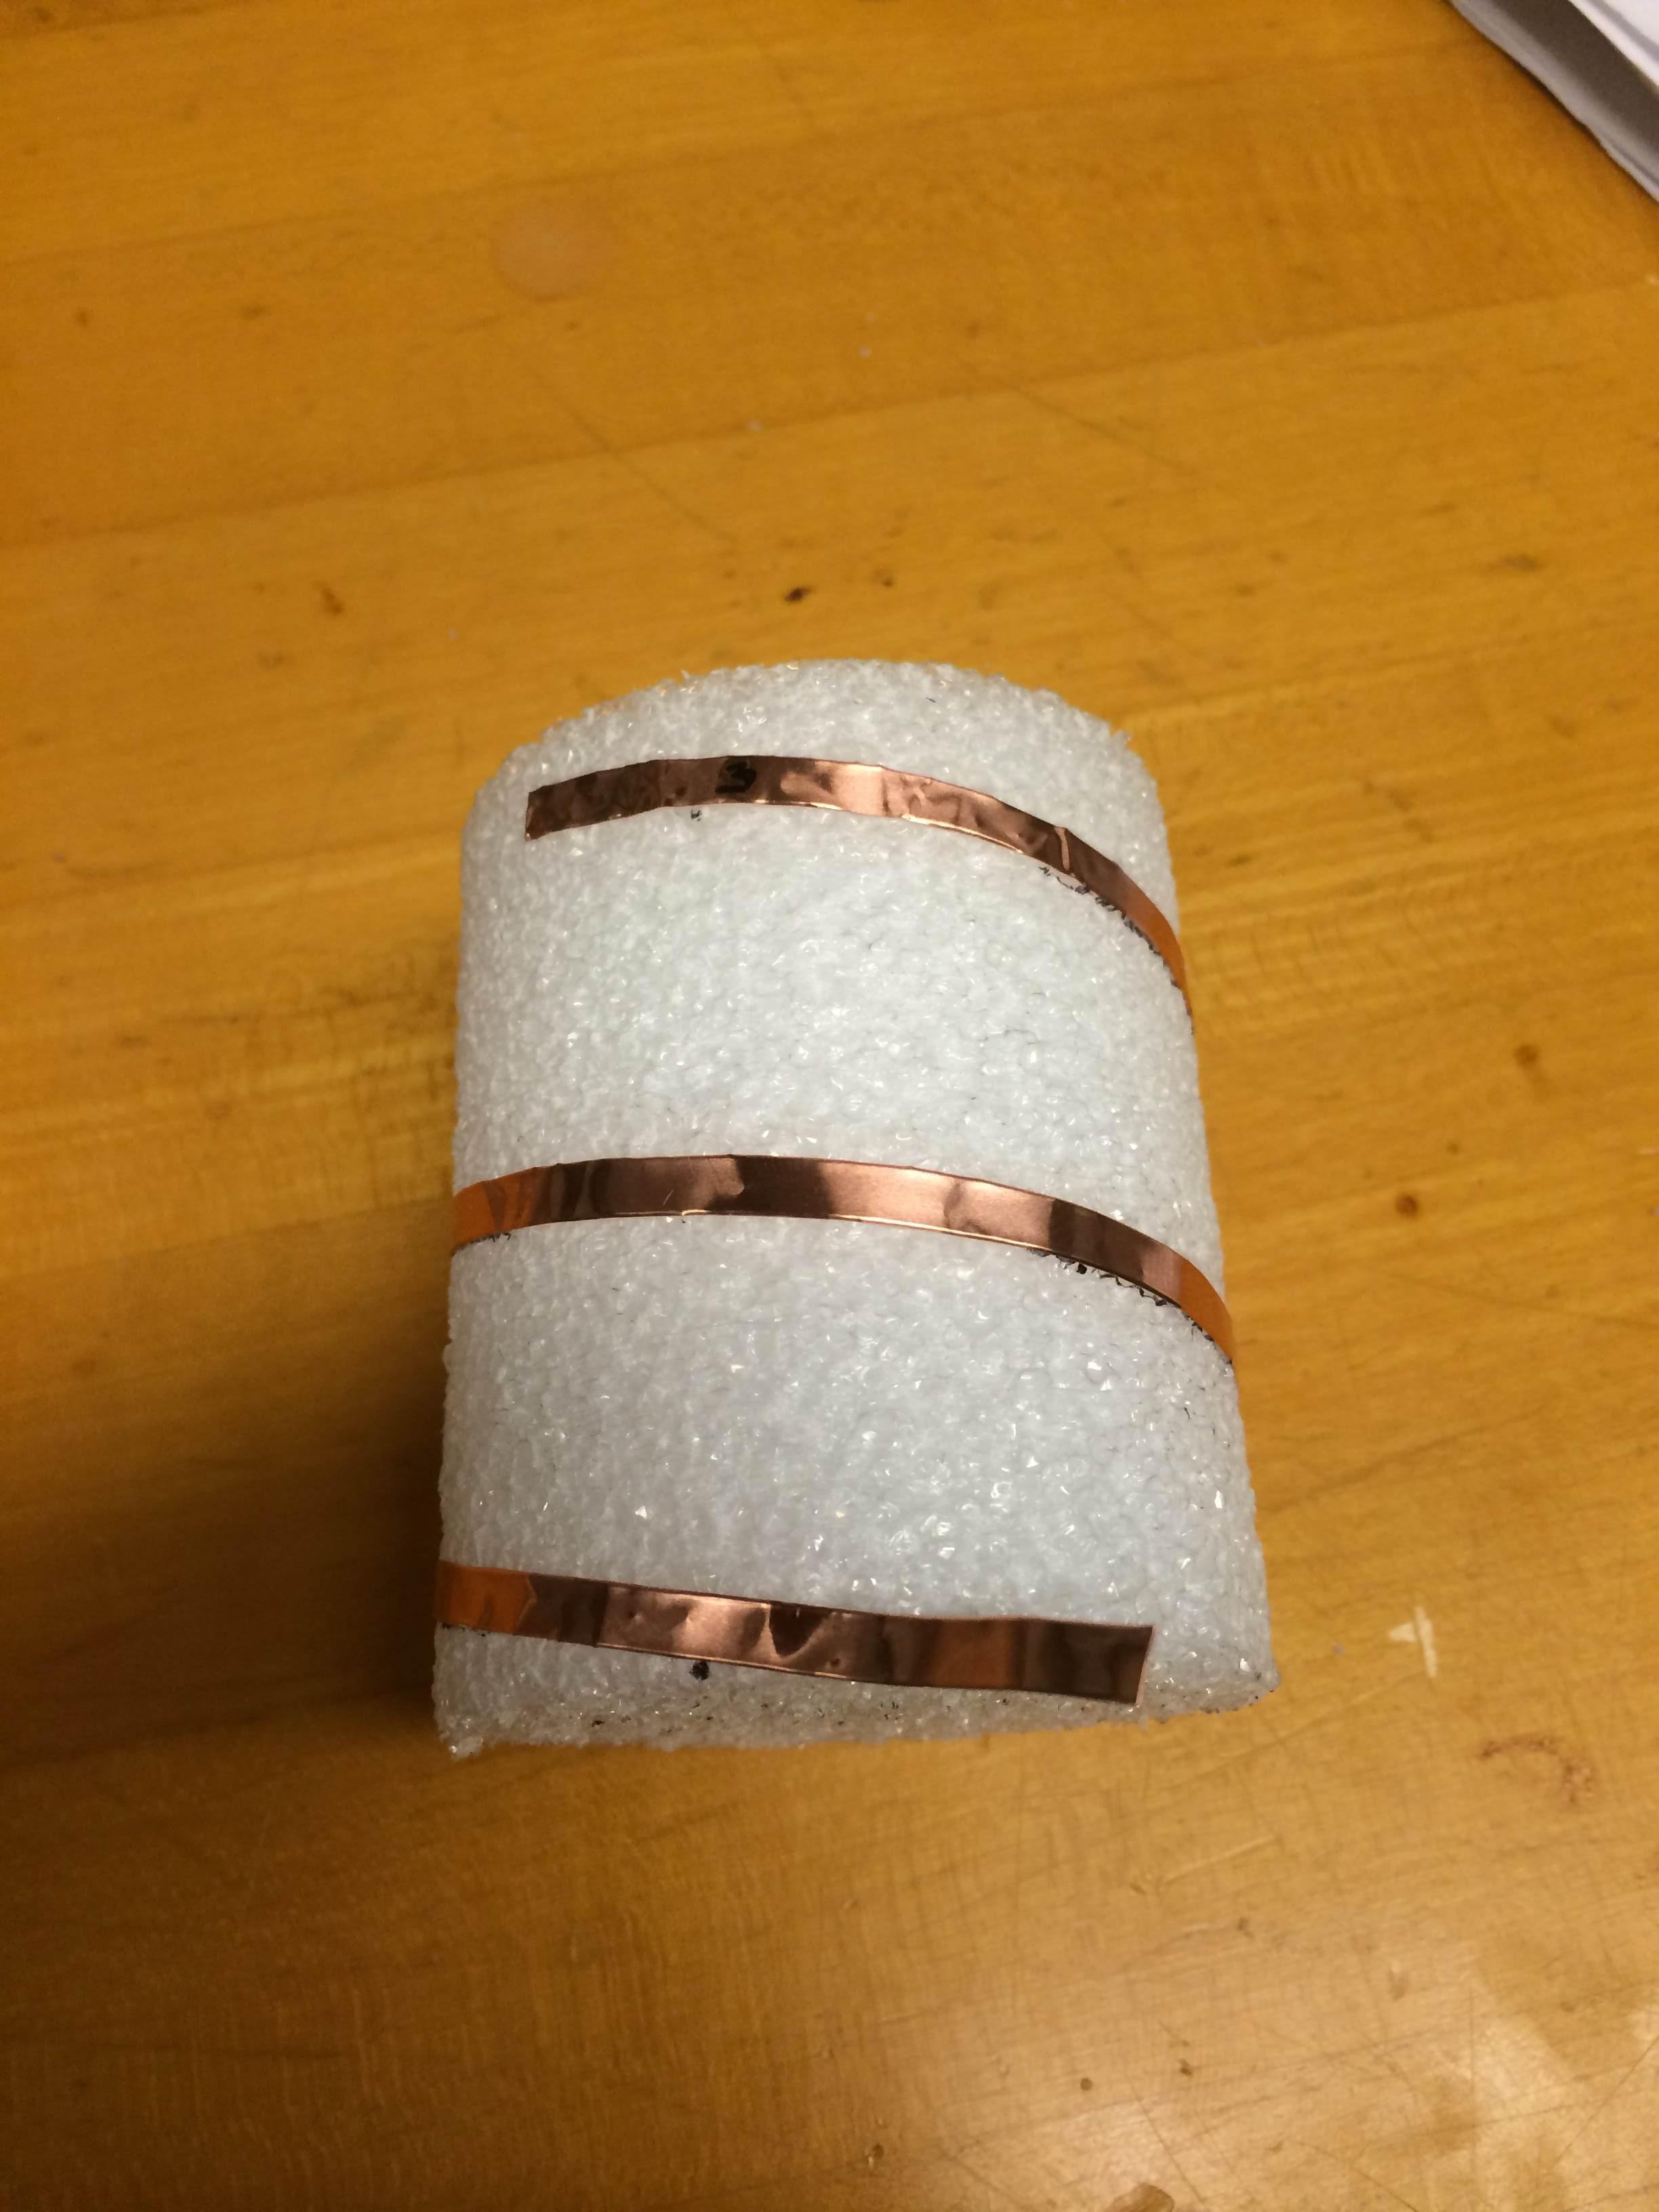
\includegraphics[scale=0.08]{feed/11.jpeg}
\end{center}


Once the tape was applied we soldered on 26.25mmx13mm piece of copper tape for impedance matching section. Note: It is important to include an extra 3-4mm on the long side of the rectangle so that it can be attached to the helix. 


In the process we melted some of the rod. This should be ok as long as the tape stays in a helix. 

\begin{center}
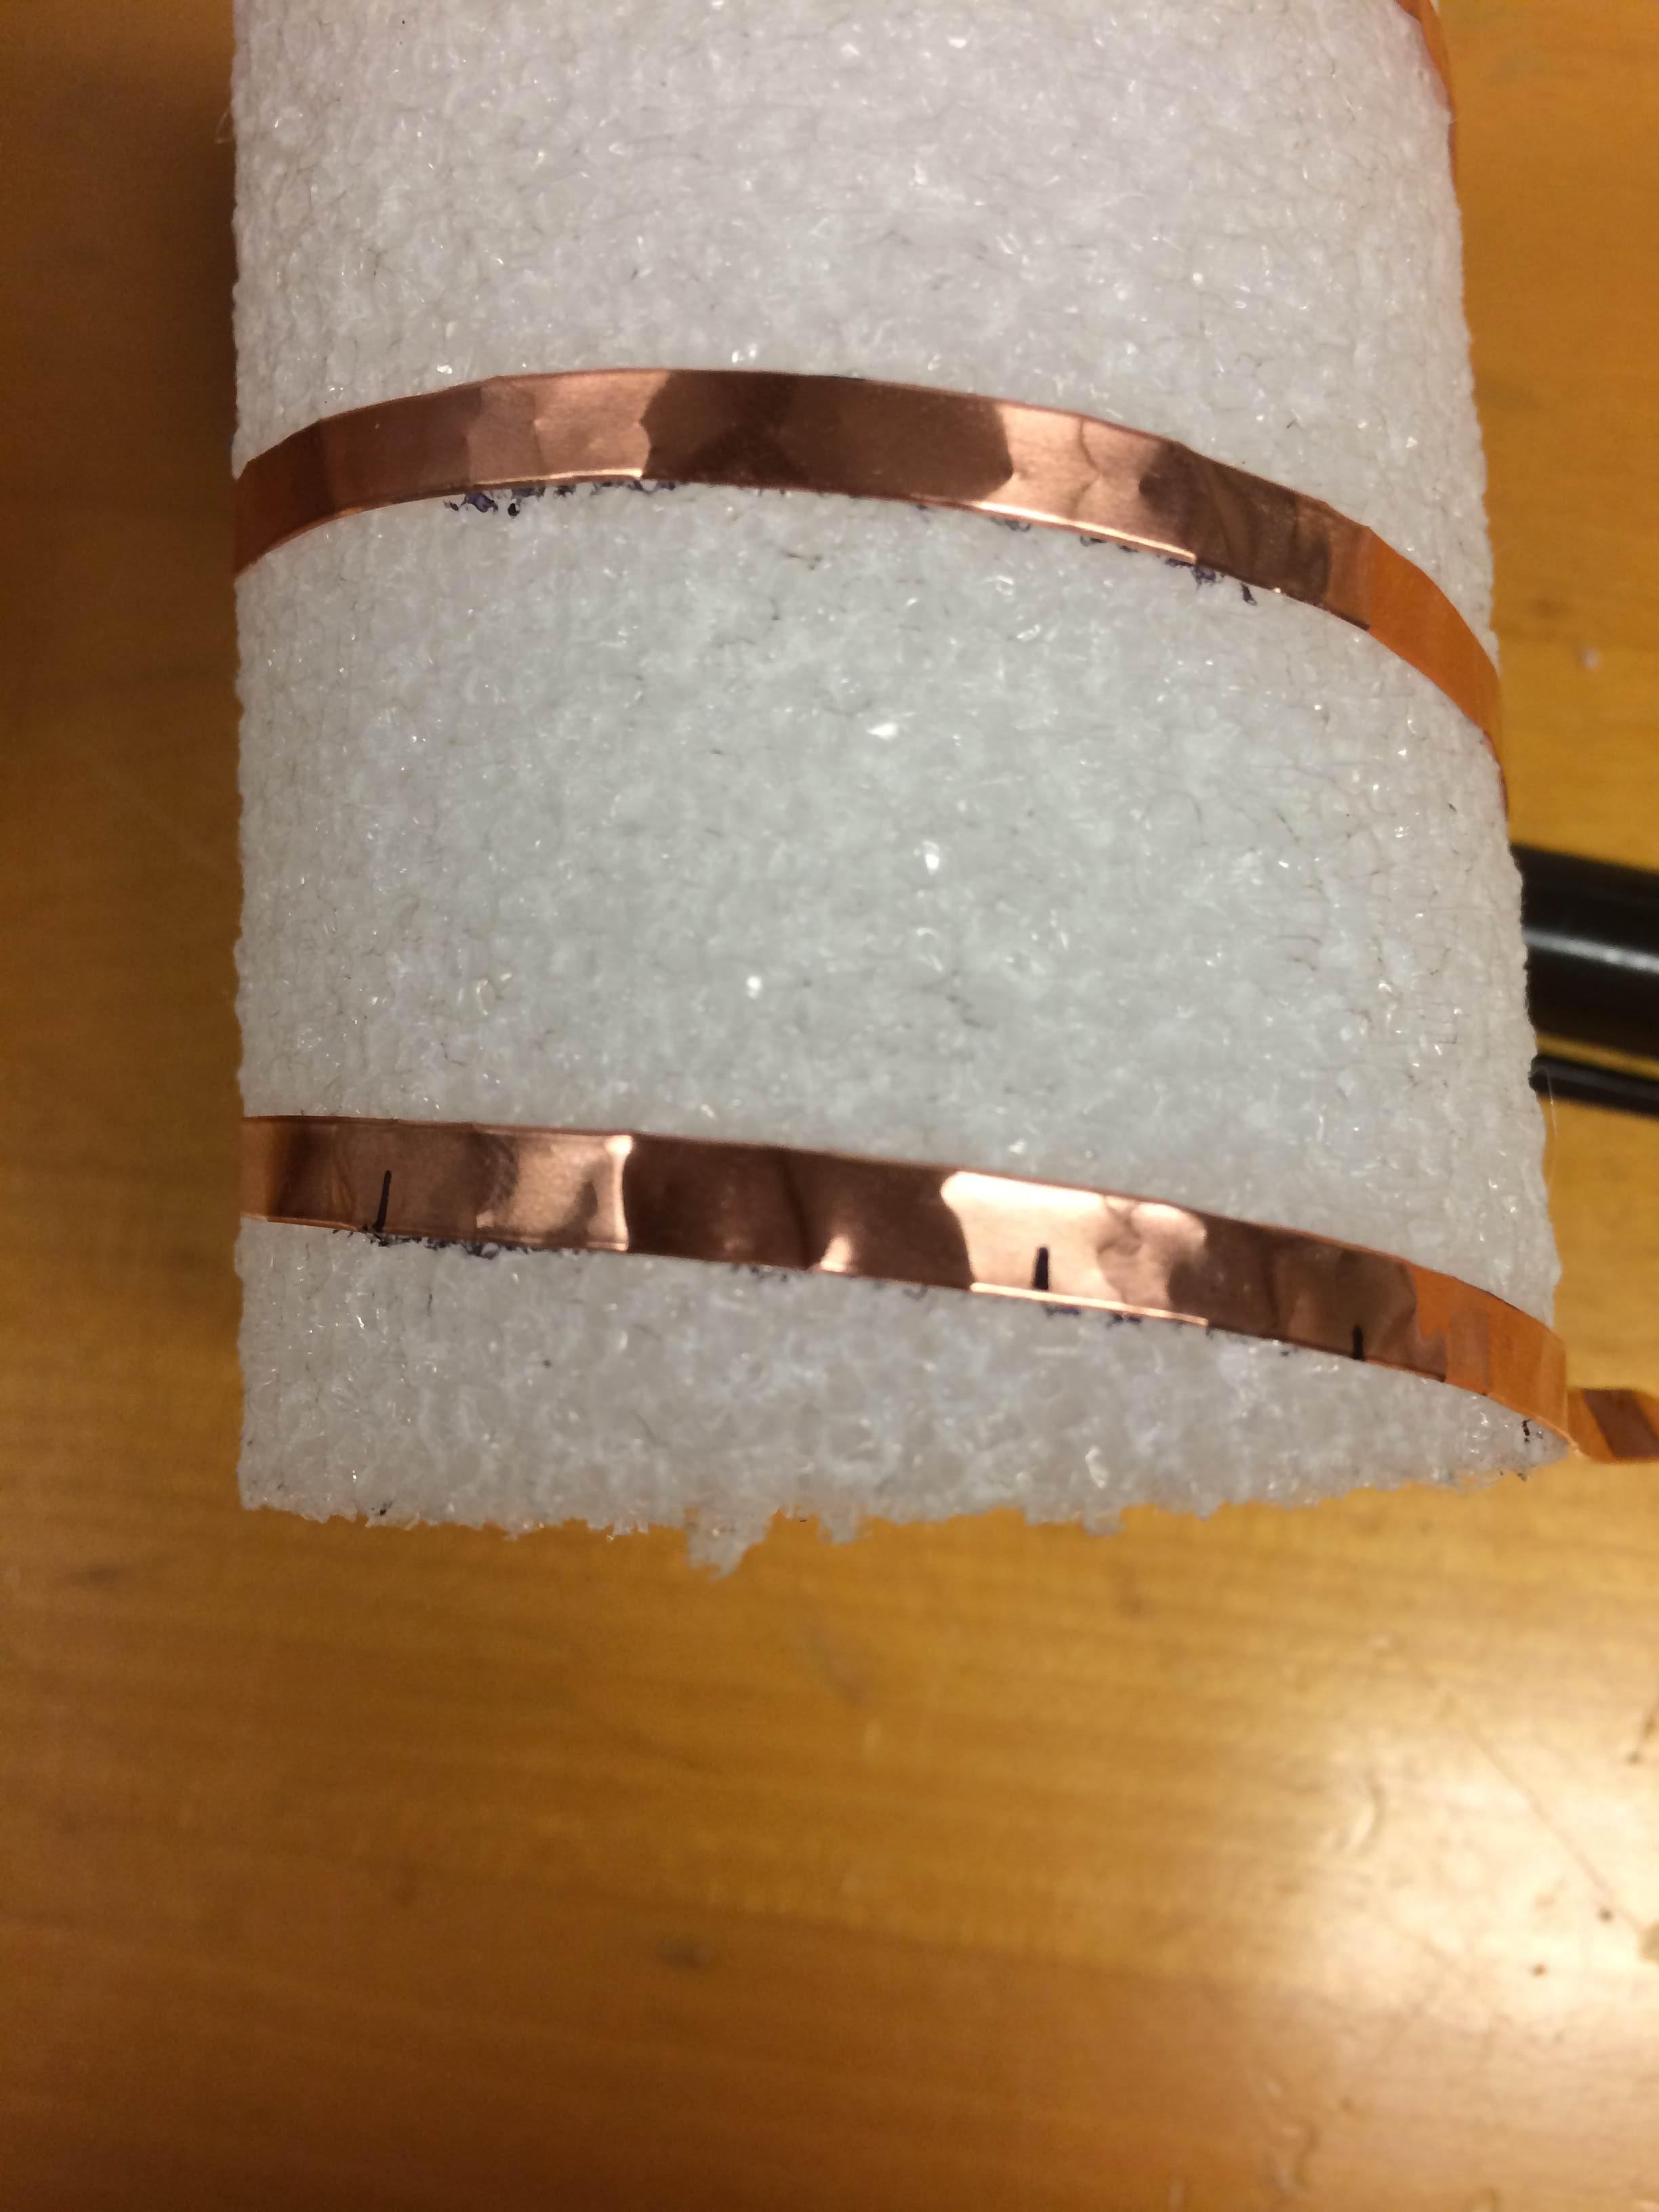
\includegraphics[scale=0.14]{feed/12.jpeg}
\end{center}


\begin{center}
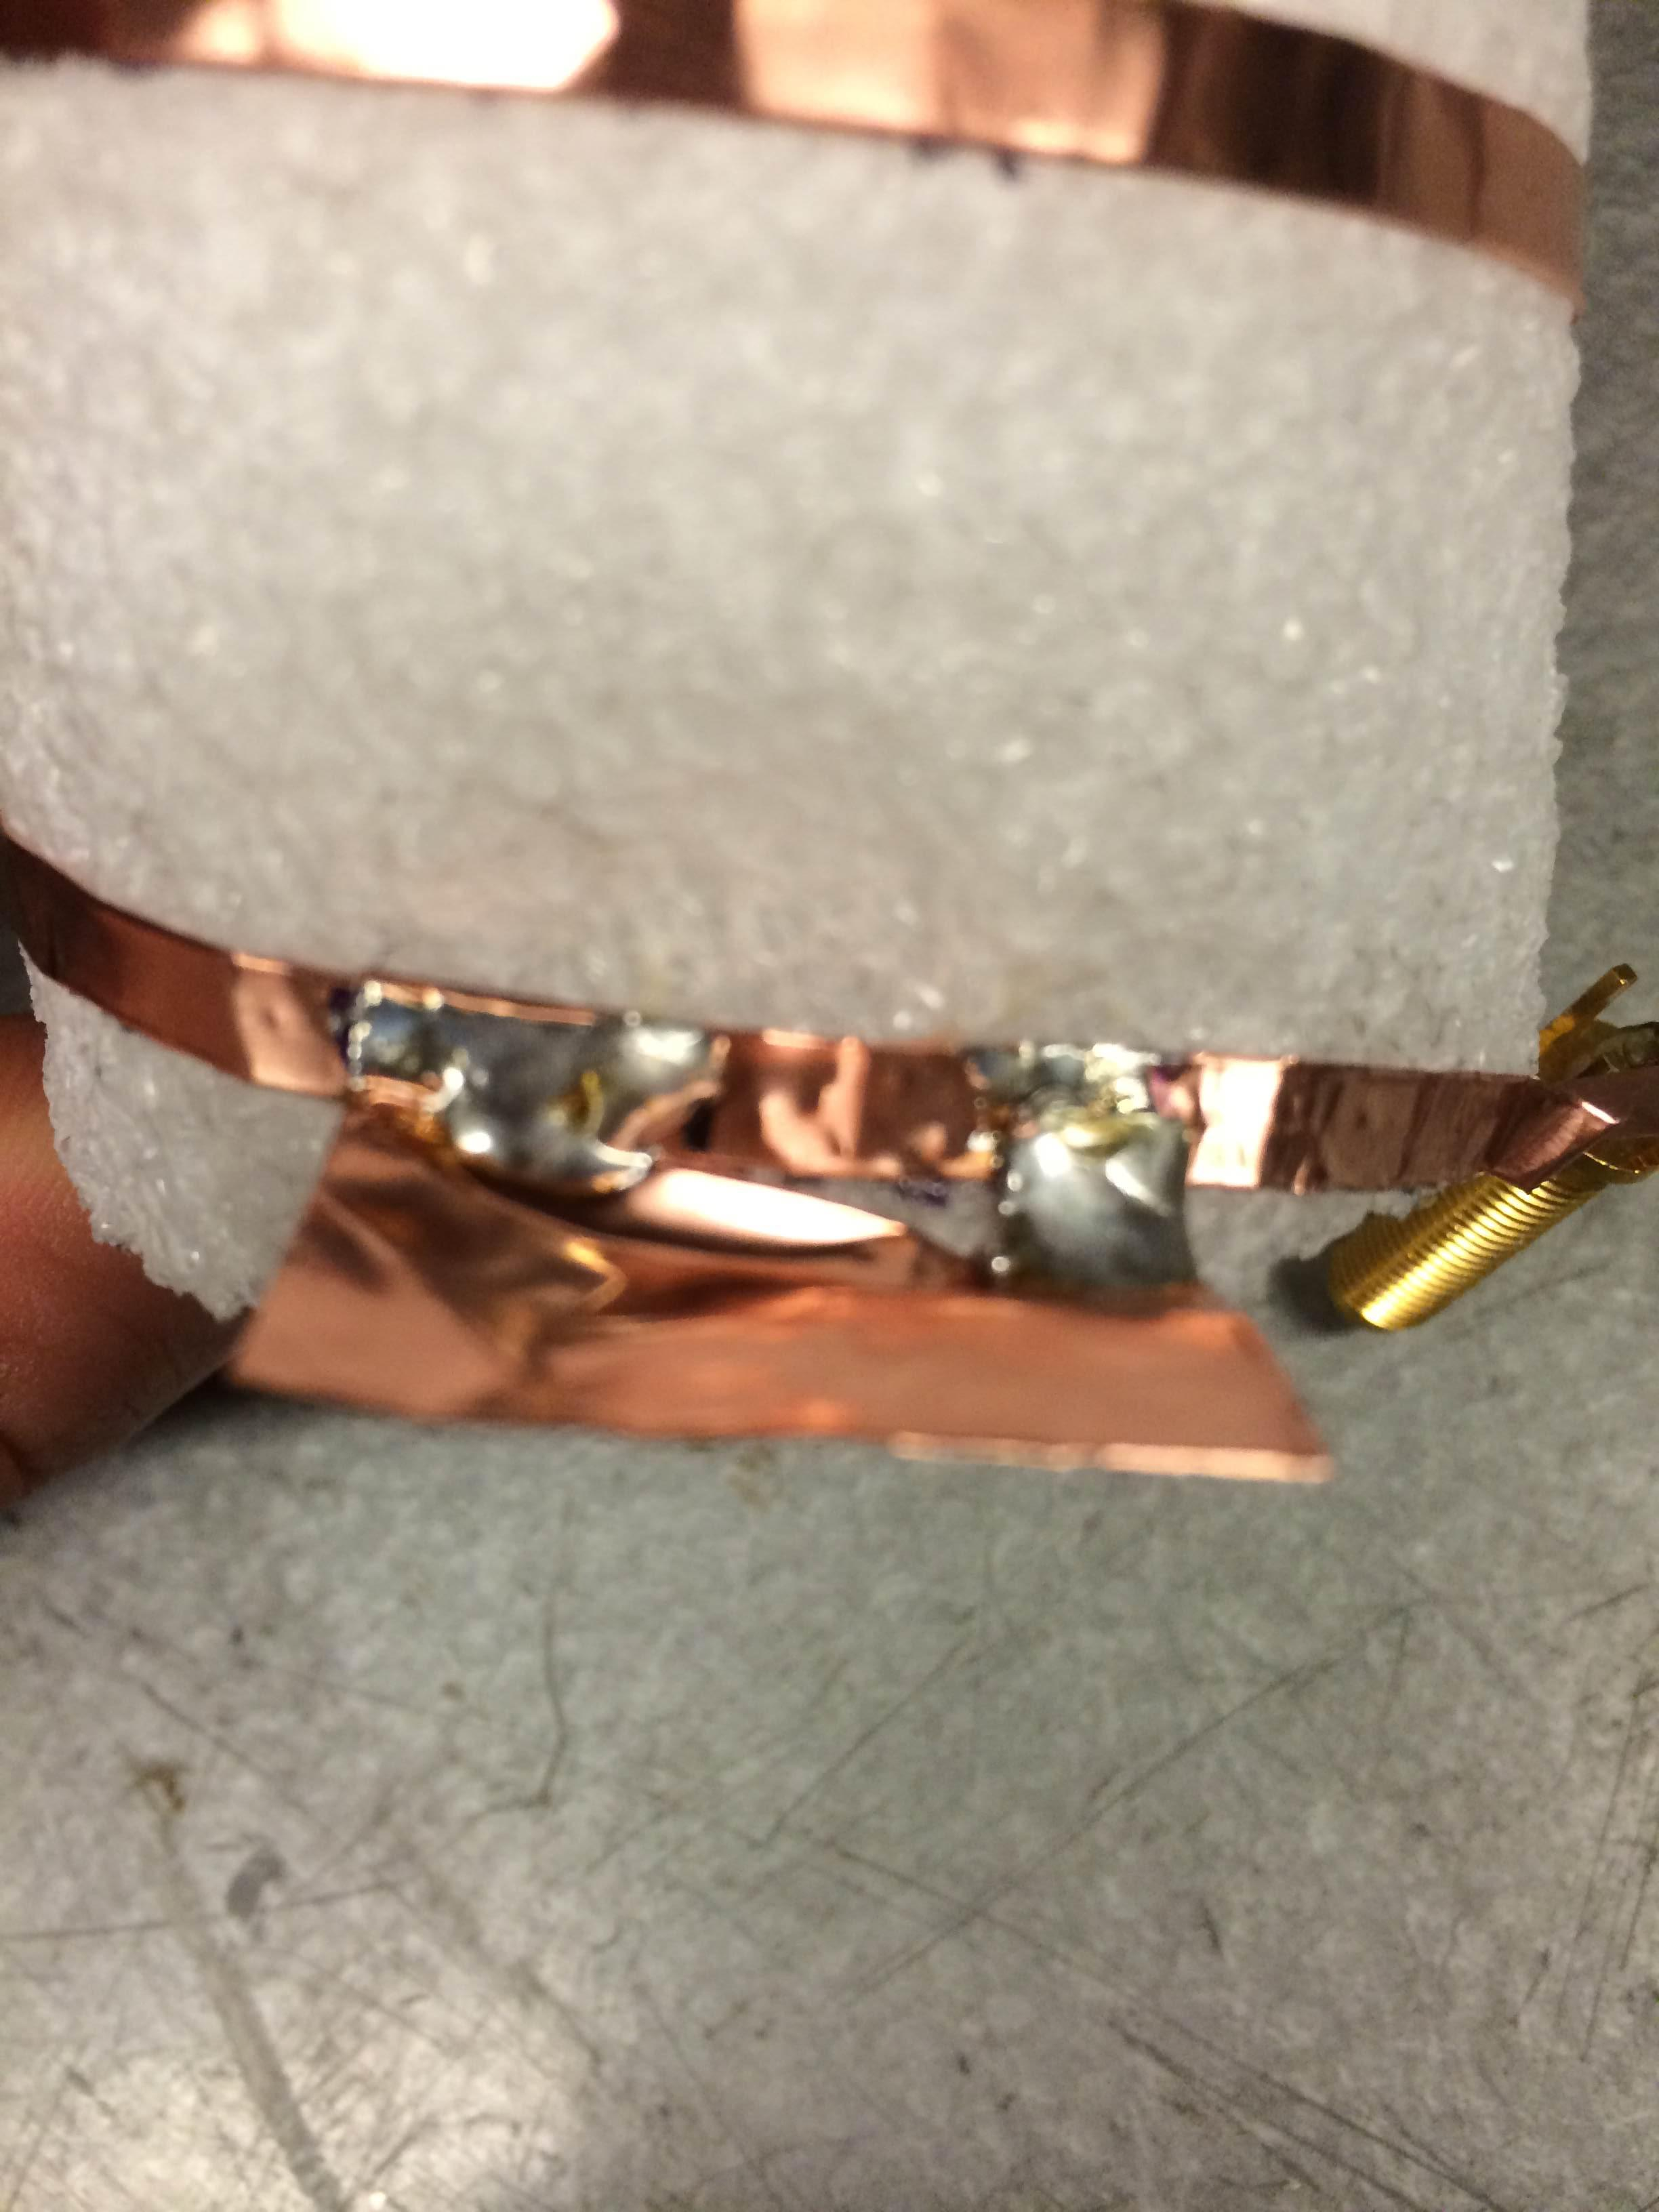
\includegraphics[scale=0.10]{feed/13.jpeg}
\end{center}


The we soldered the end of the helix to the SMA connector. MIT cut off some of the ground pins to make that easier. We left them on and it worked out the same. 

\begin{center}
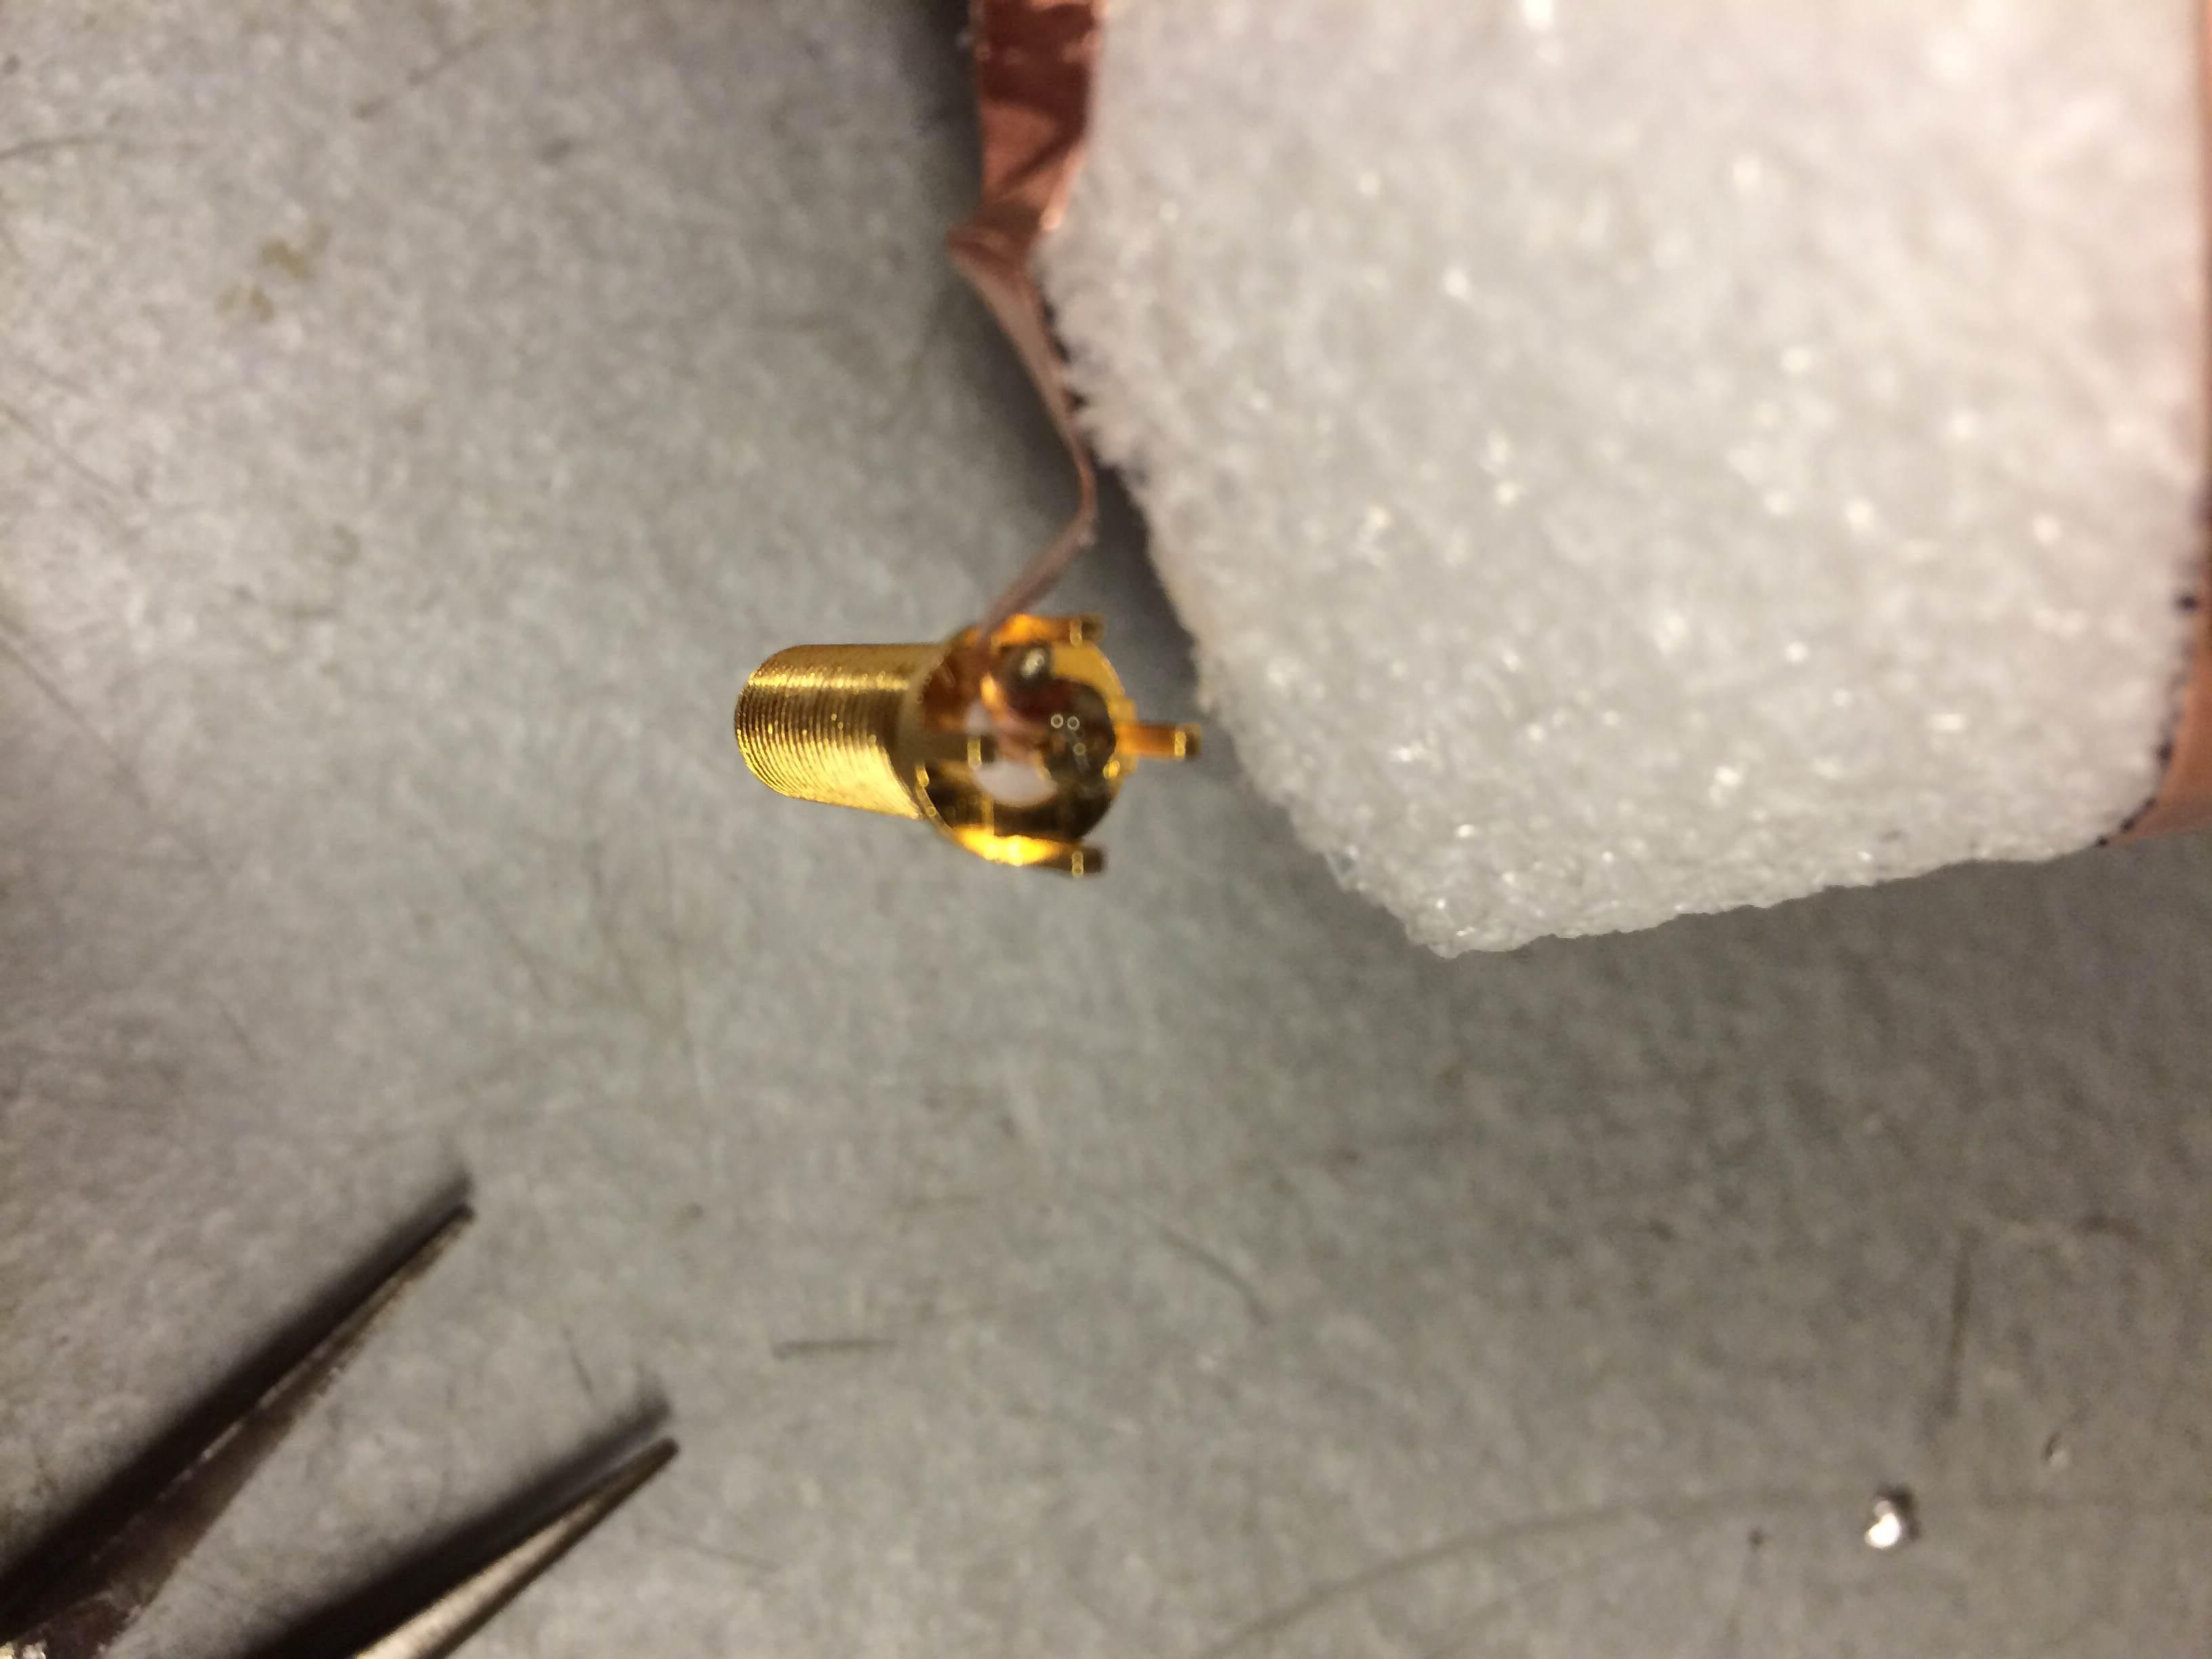
\includegraphics[scale=0.10]{feed/14.jpeg}
\end{center}


\subsubsection{Drilling/cutting PC board}
We cut the PC board into 63mm squares (We had enough PC board to make a couple back ups). 

\begin{center}
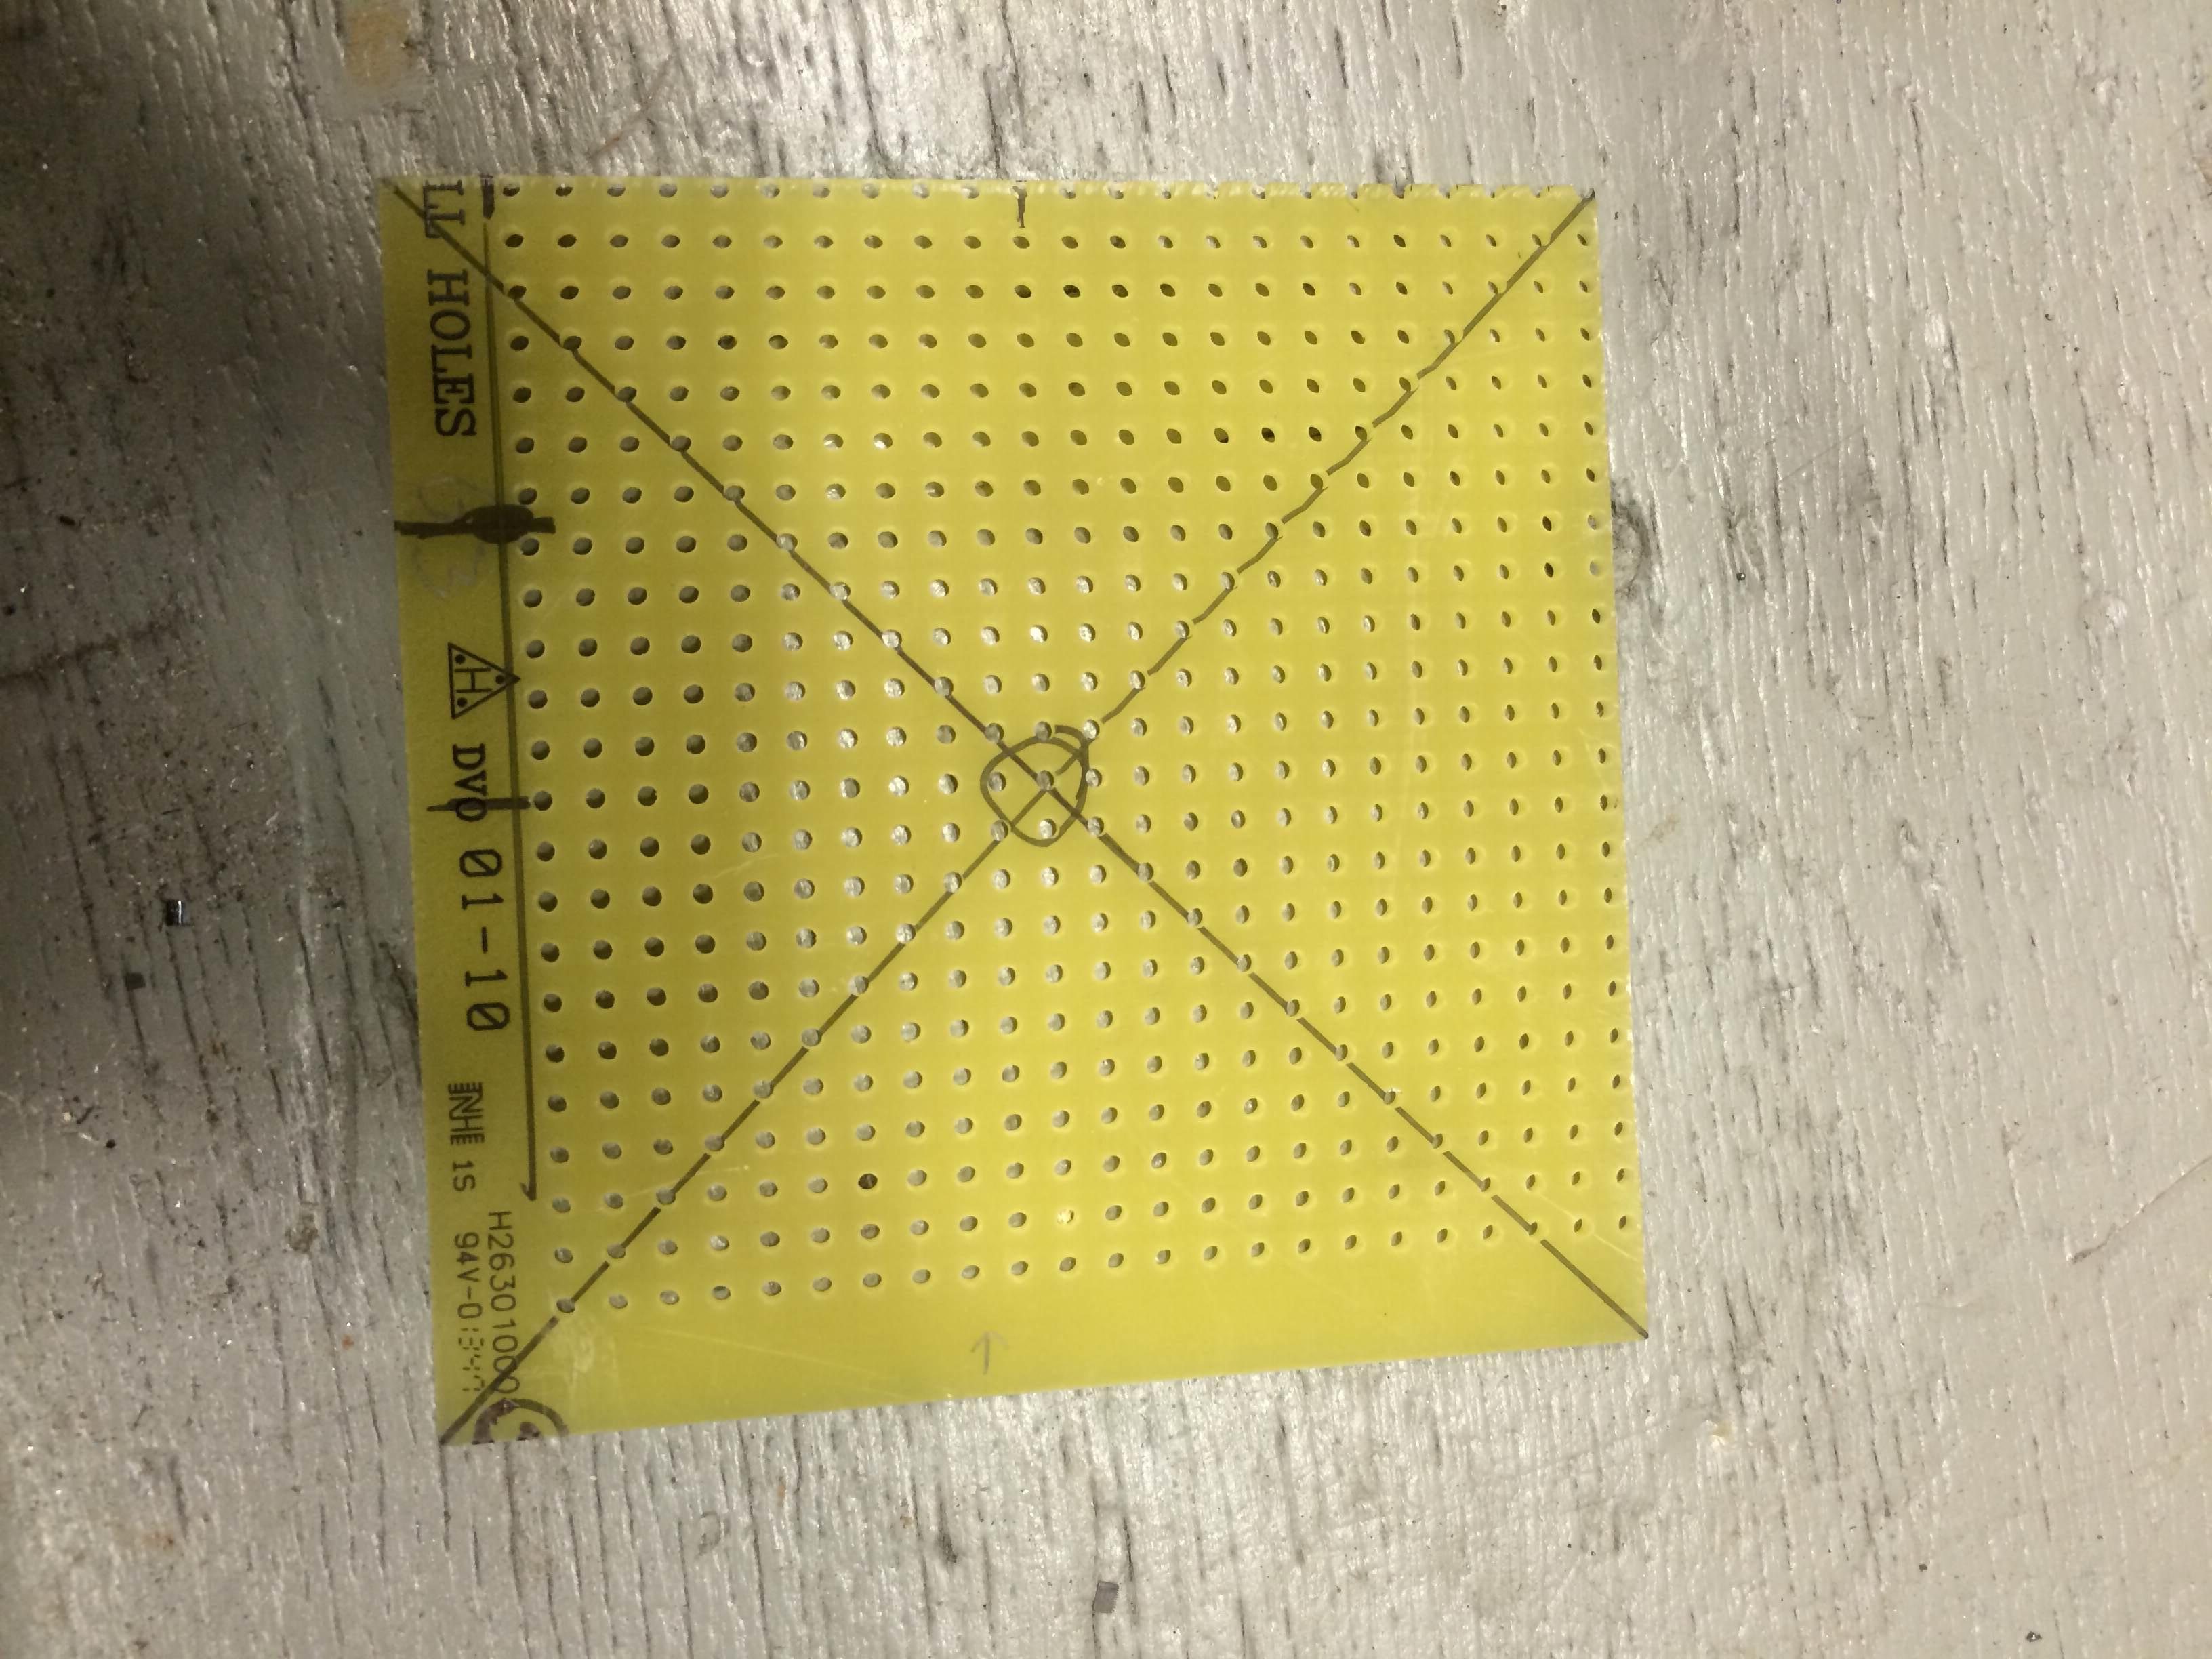
\includegraphics[scale=0.08]{feed/15.jpeg}
\end{center}


Then we drilled holes in it as specified by the manual using a drill press. It was relatively easy to secure the board in a vice for drilling. 

\begin{center}
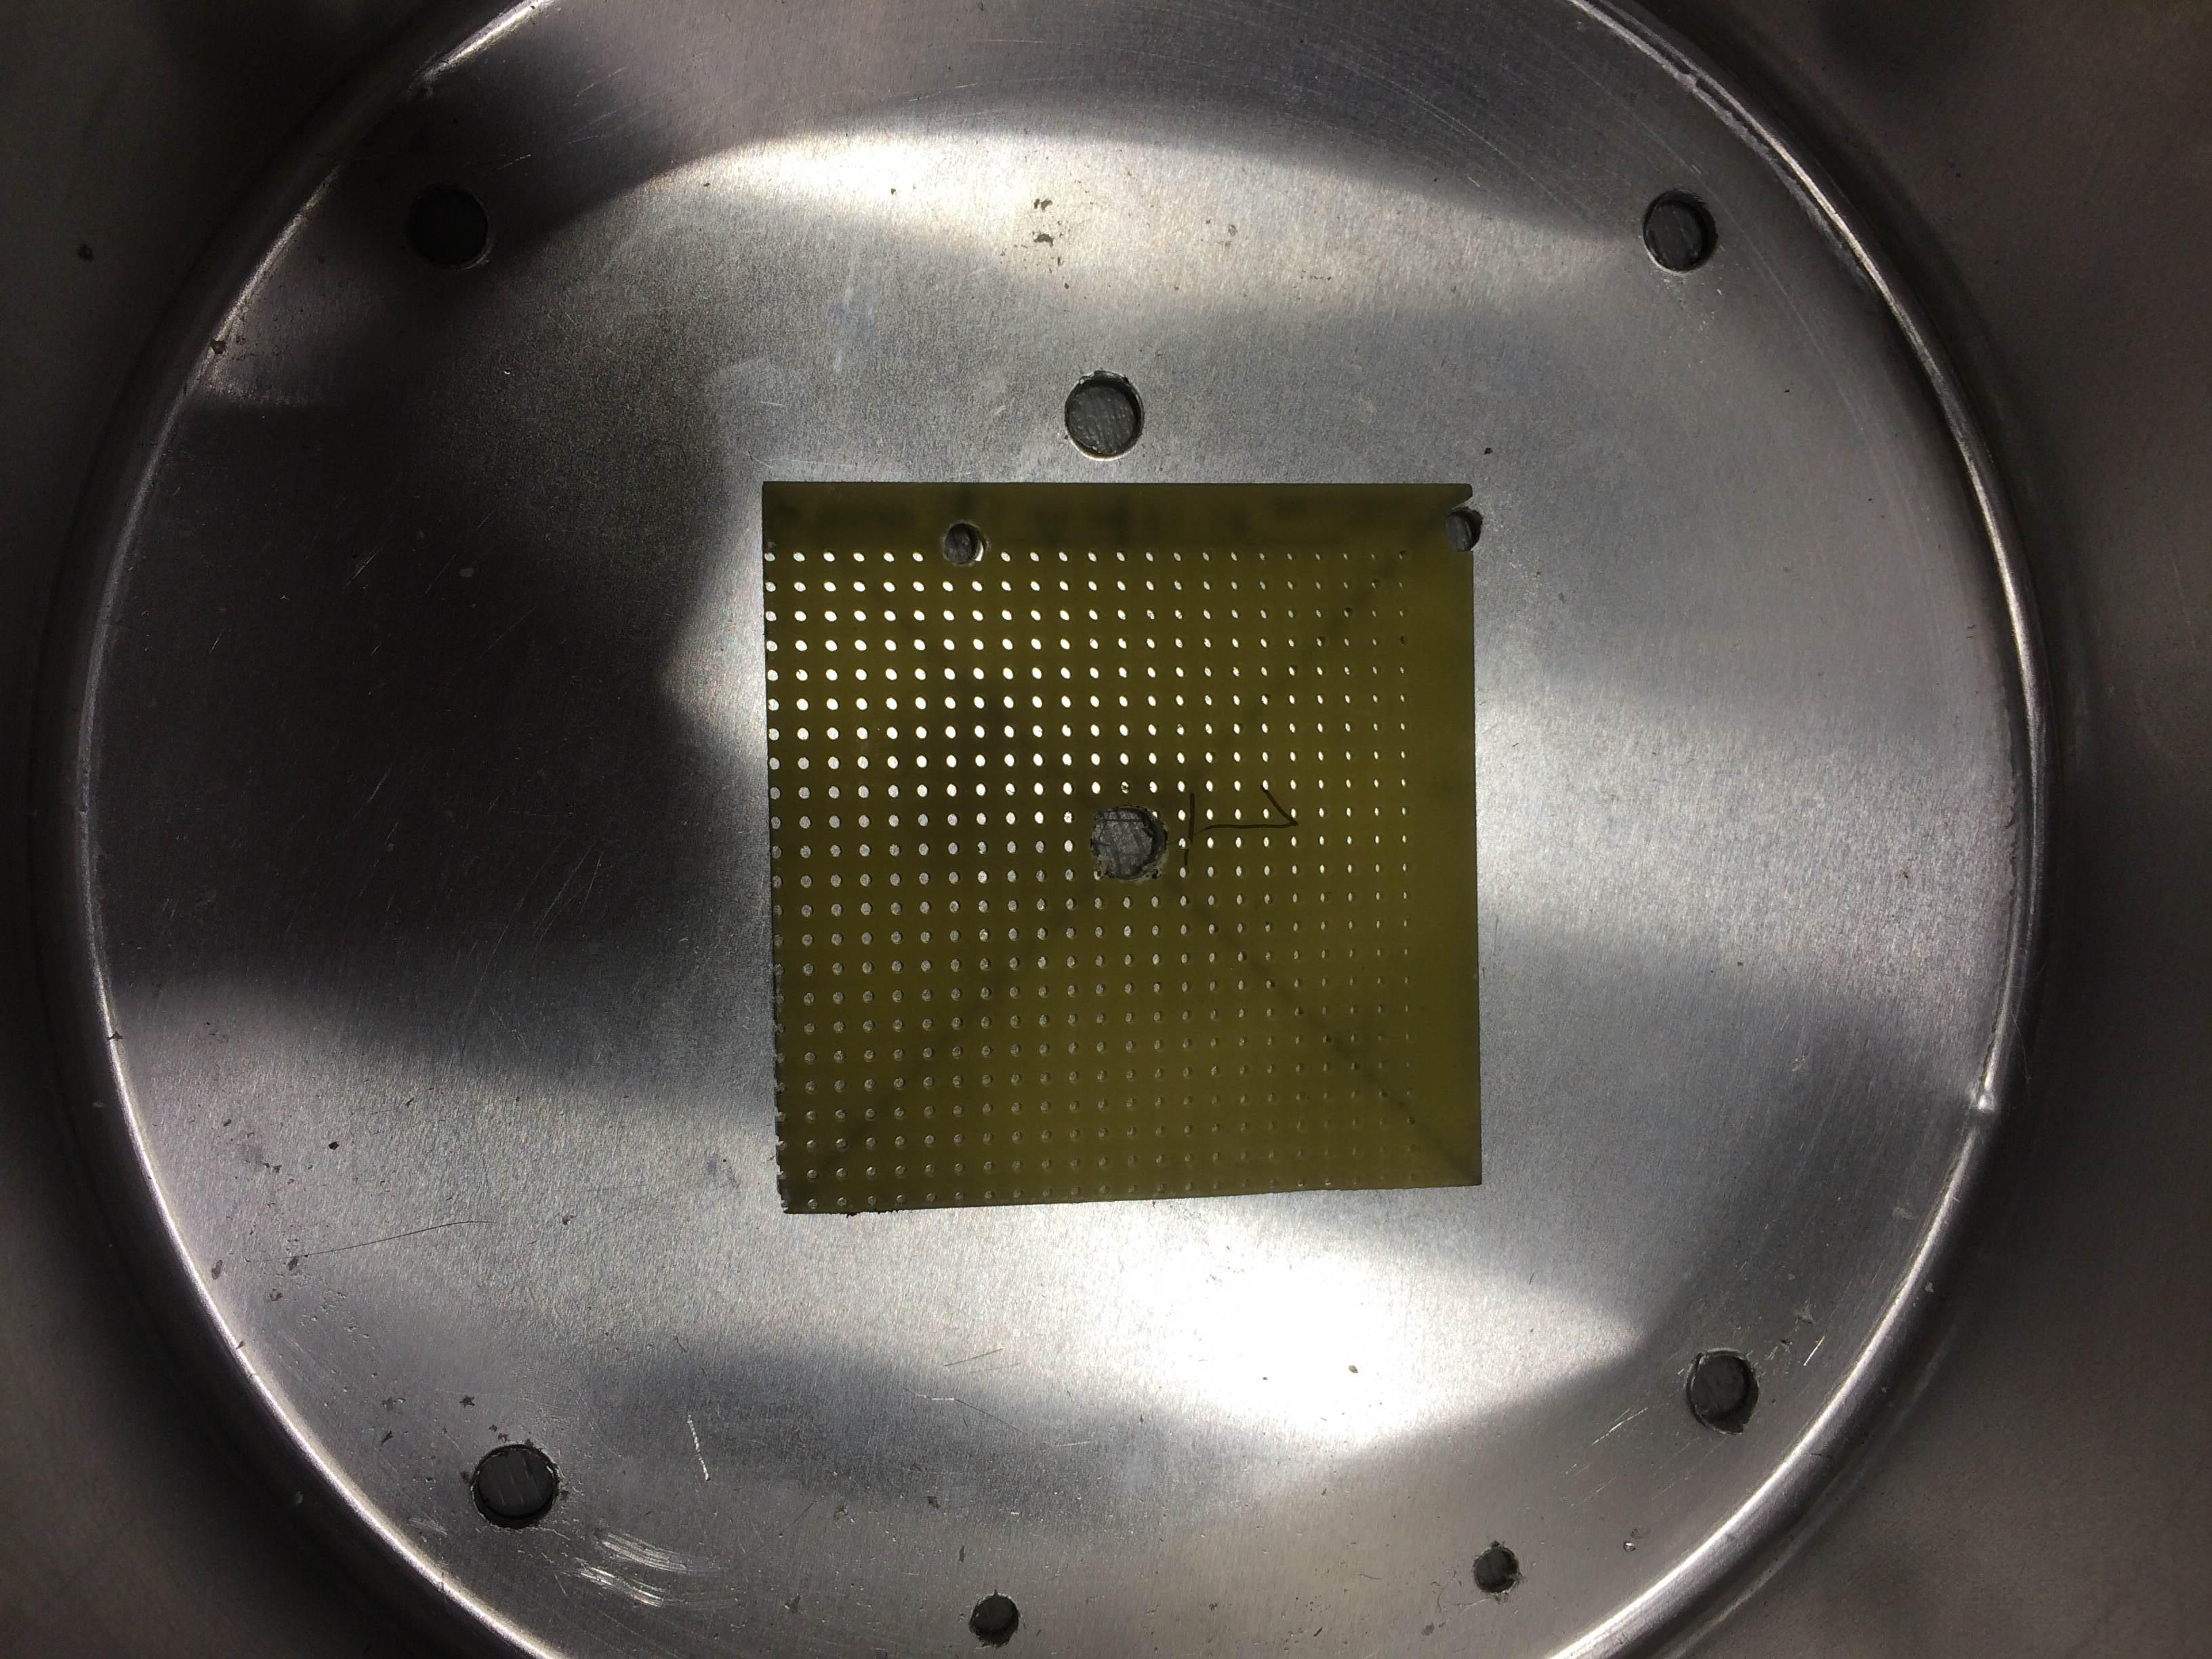
\includegraphics[scale=0.08]{feed/16.jpeg}
\end{center}


\subsubsection{Assembly}
All the components were then bolted together. 

\begin{center}
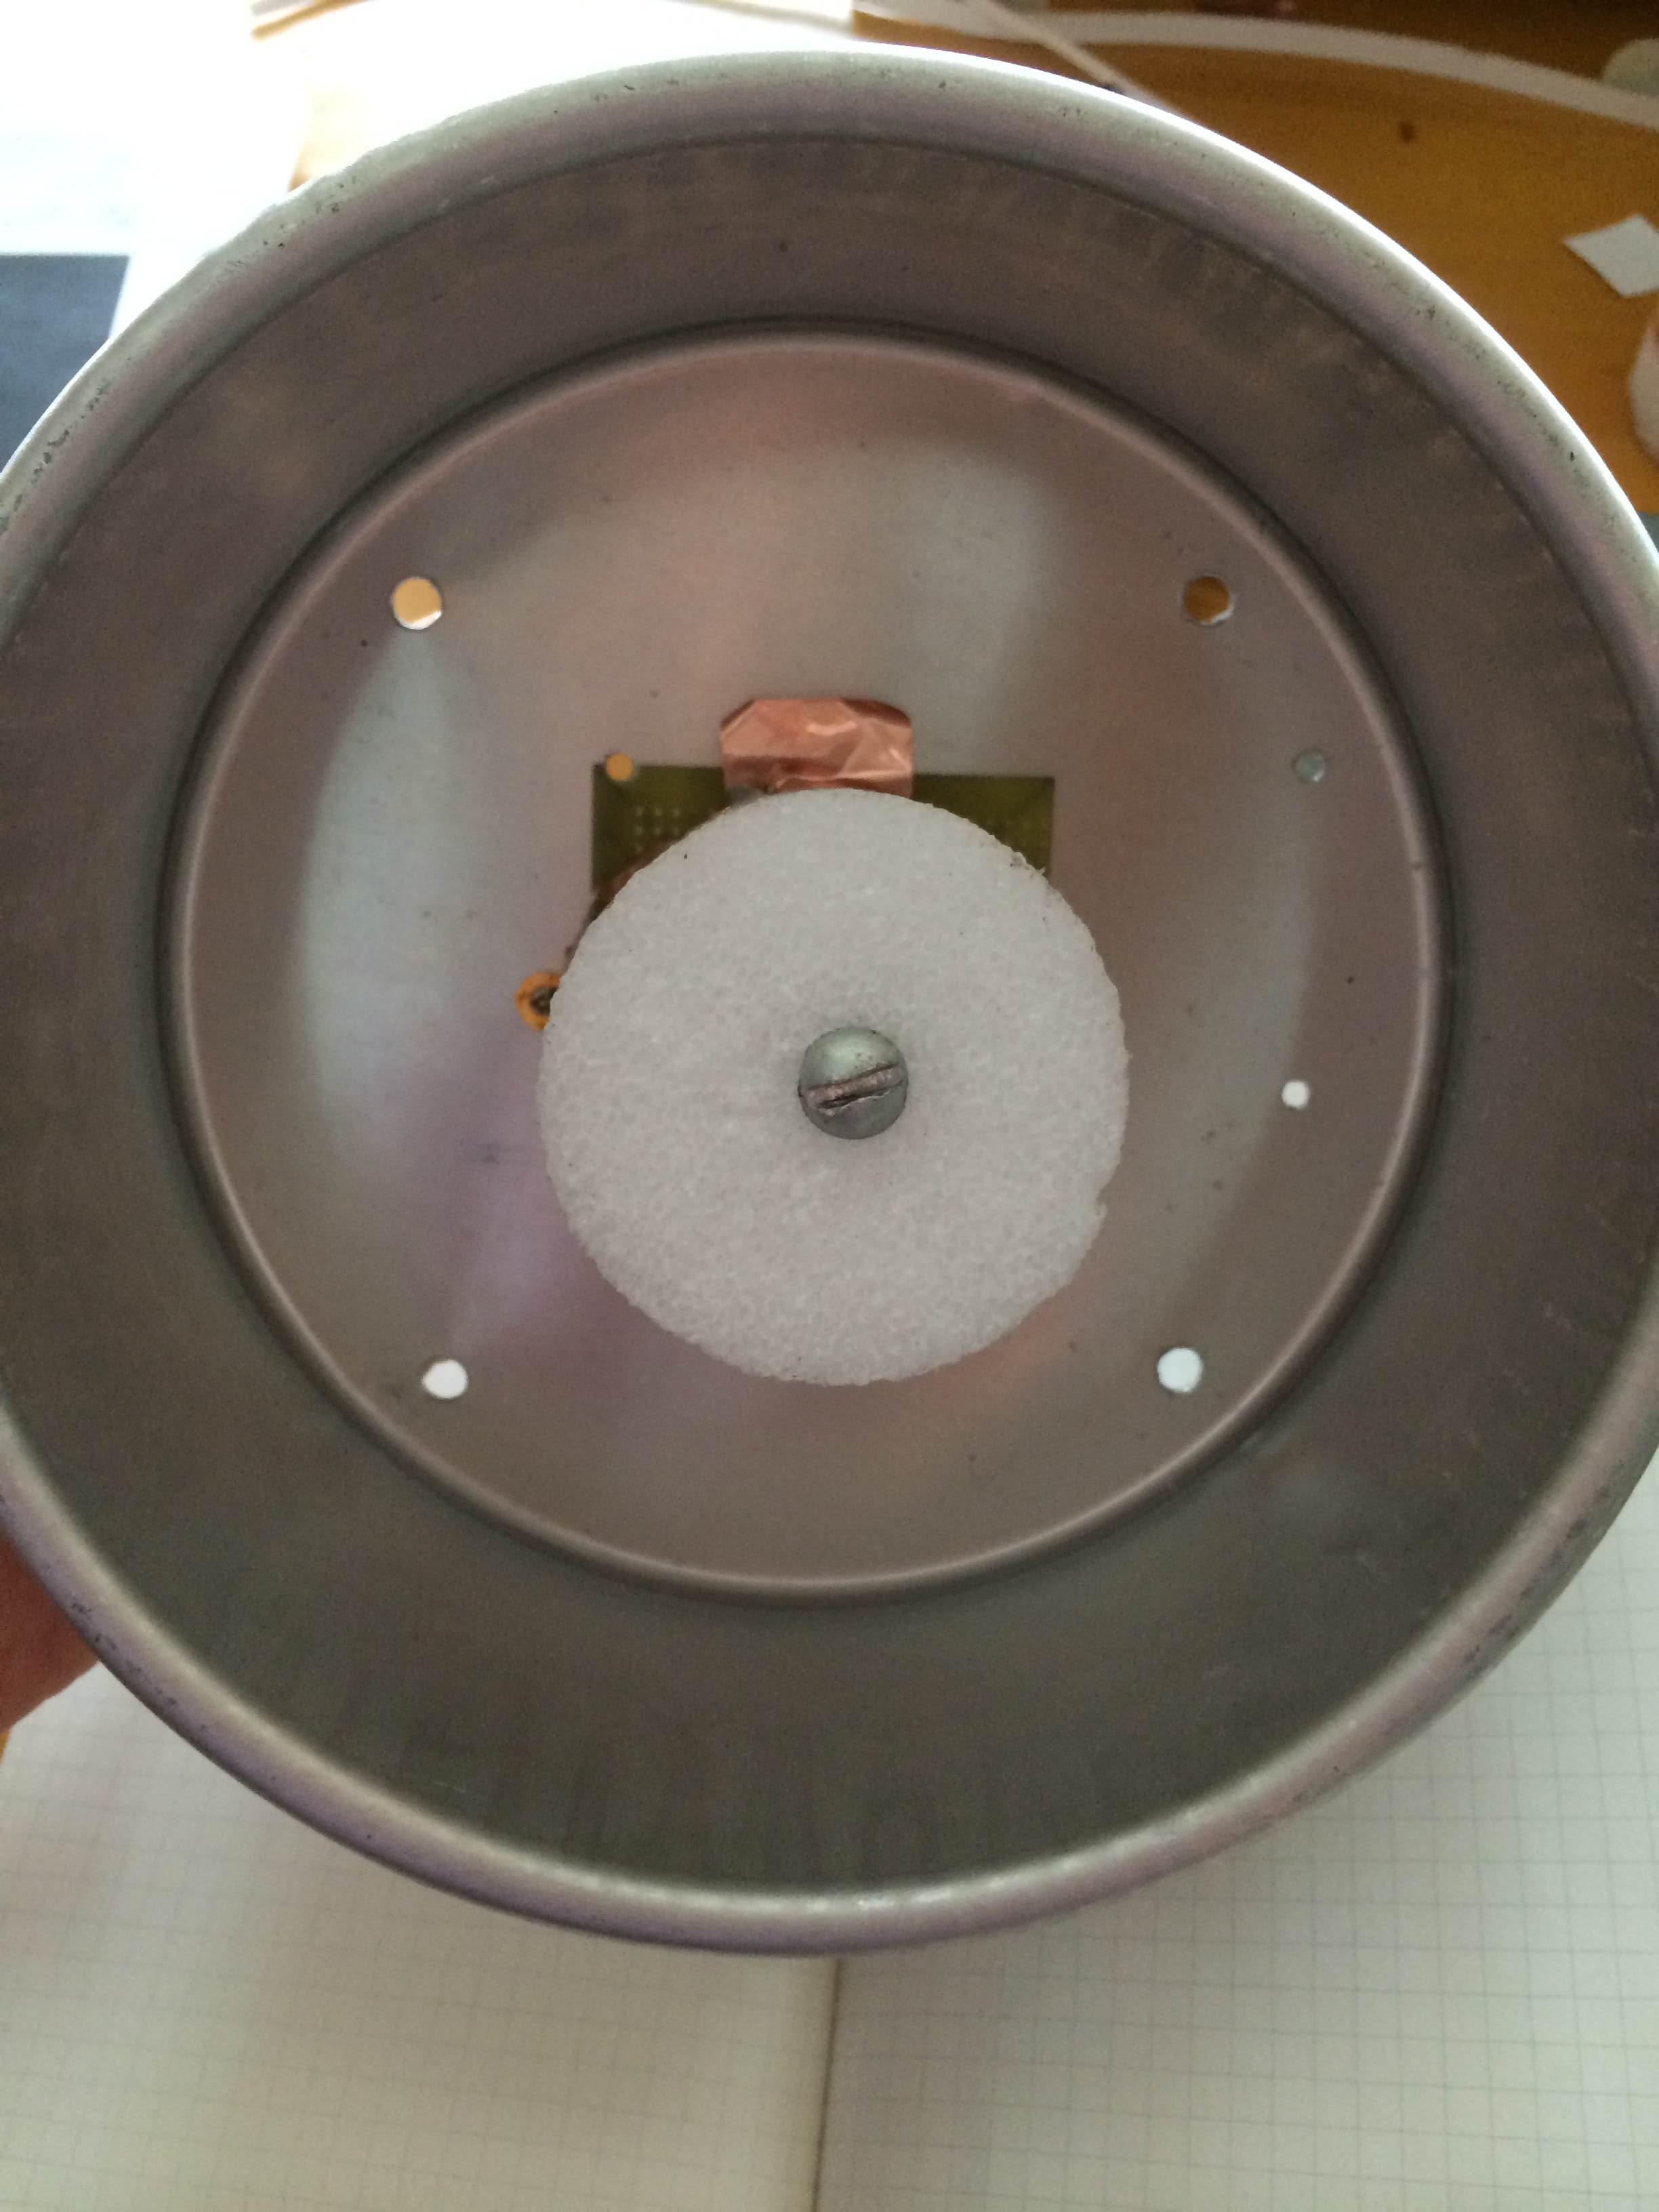
\includegraphics[scale=0.08]{feed/17.jpeg}
\end{center}

\begin{center}
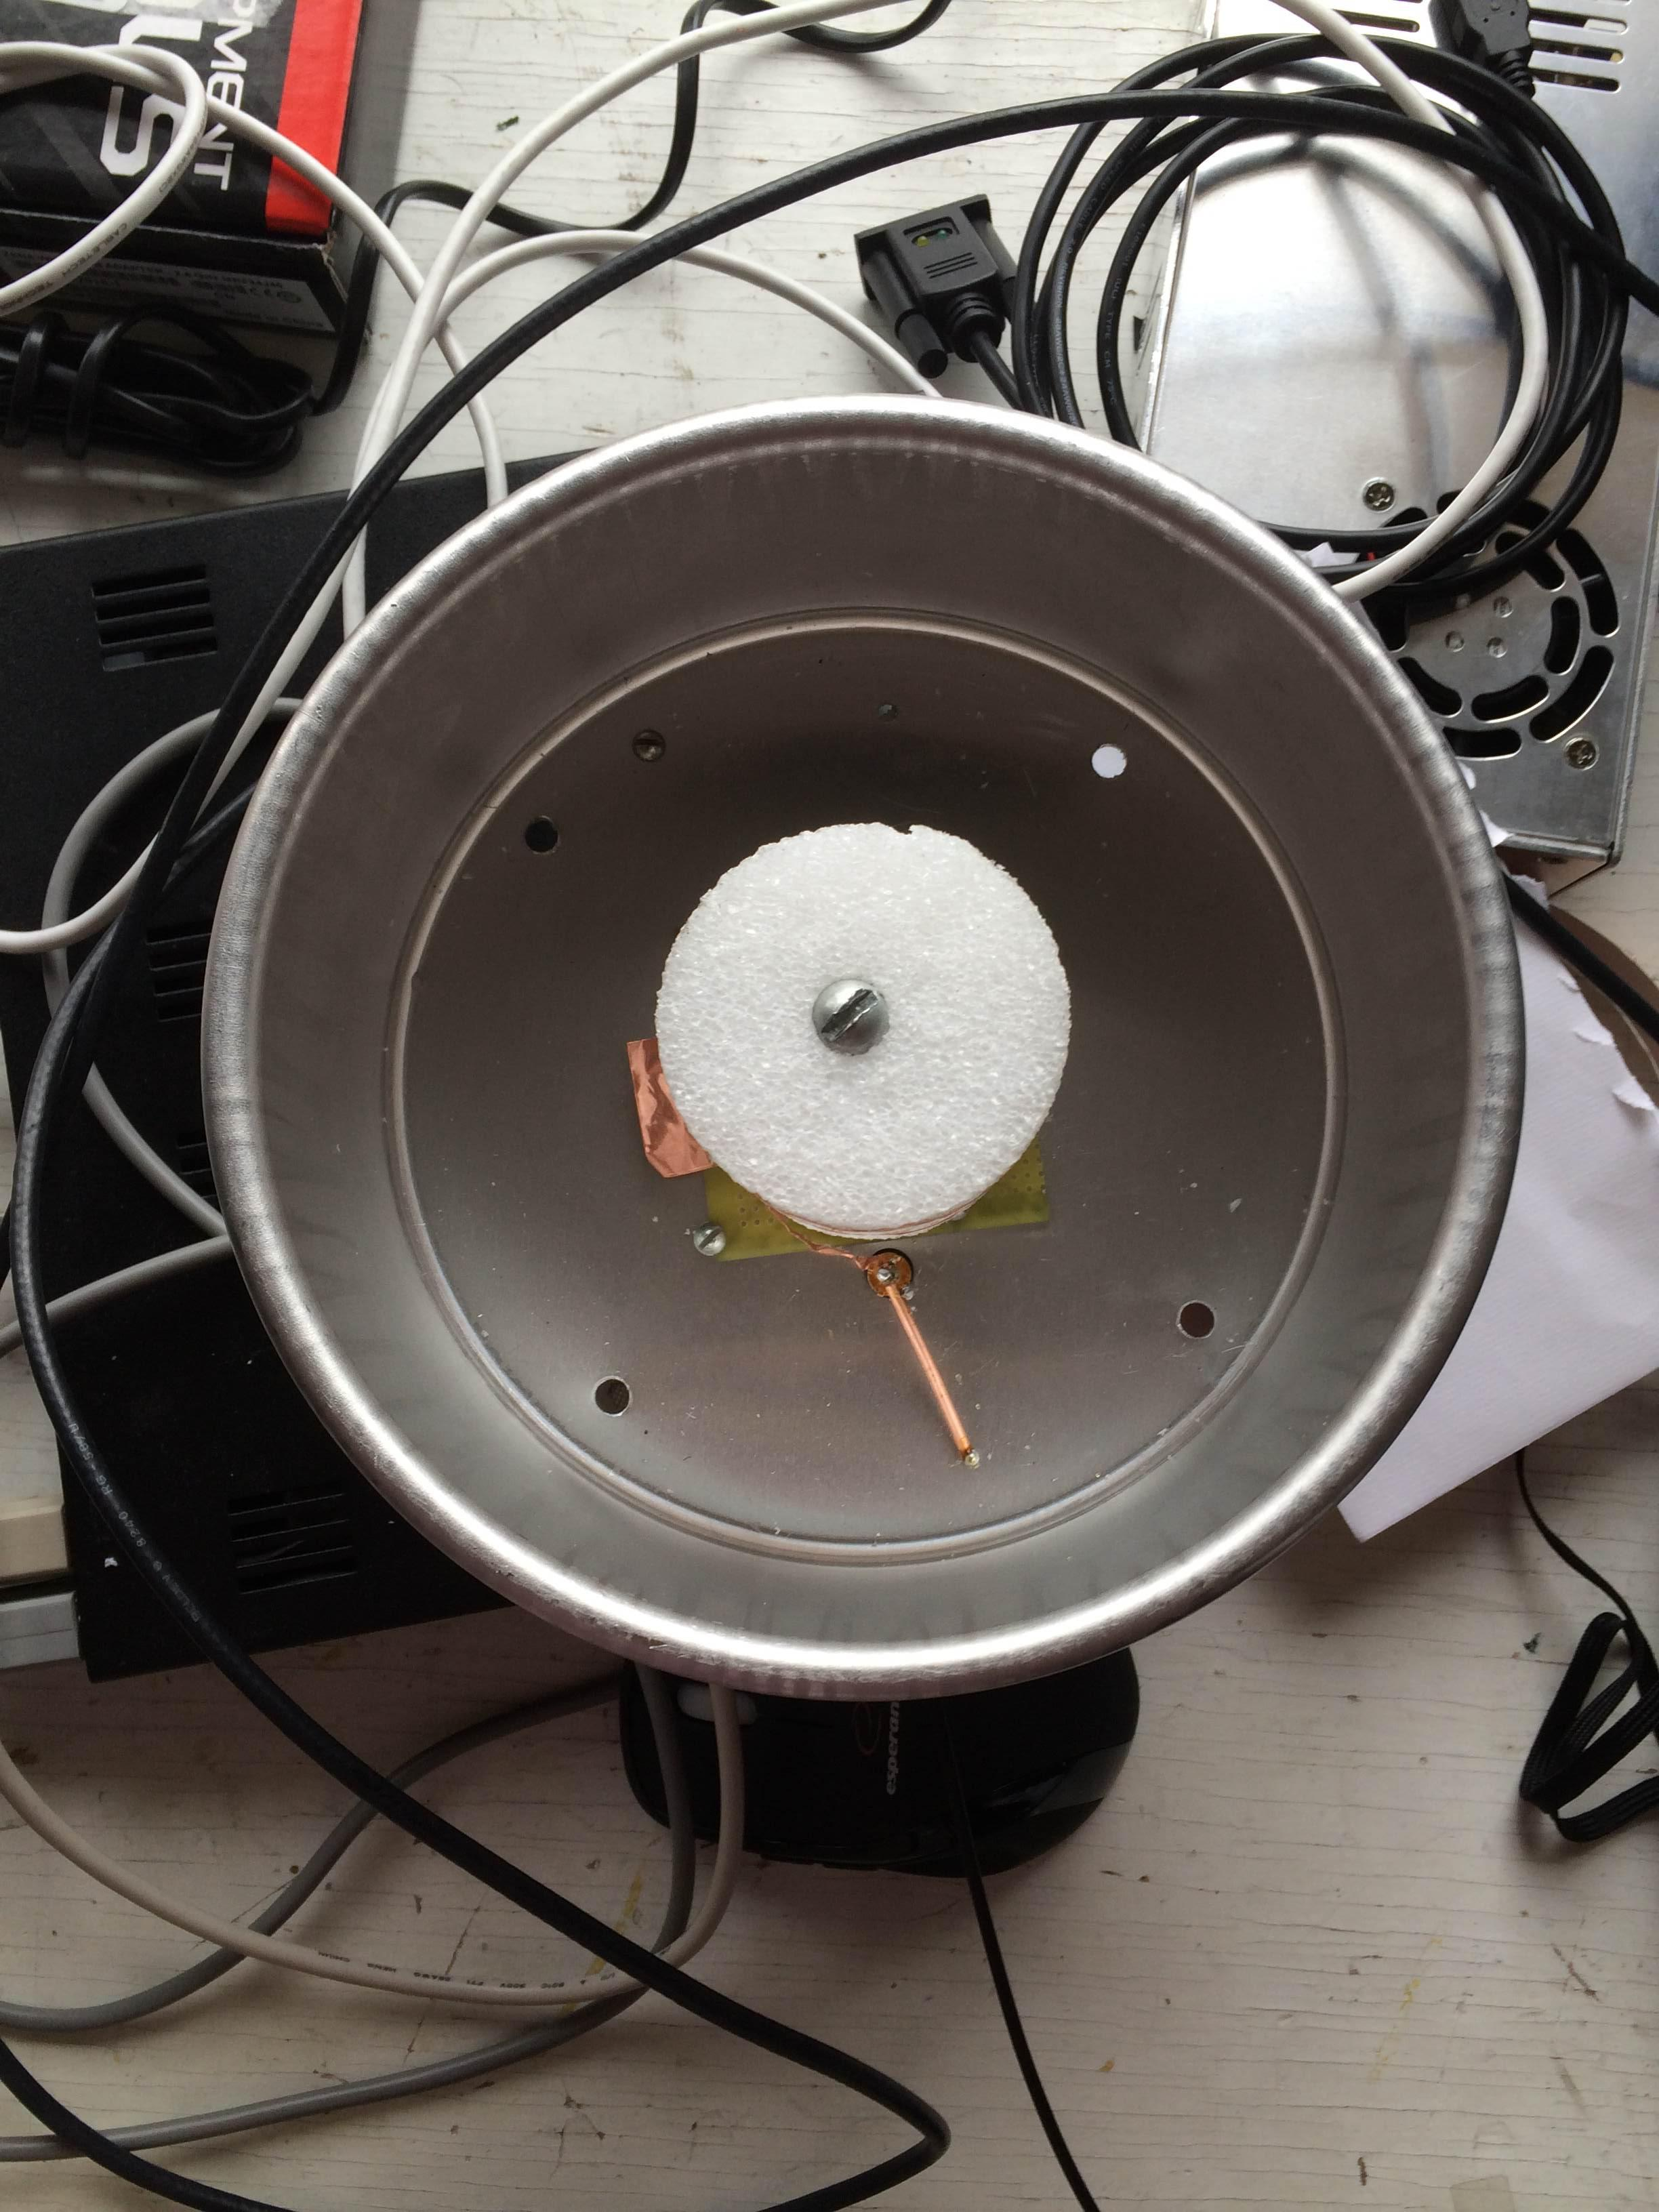
\includegraphics[scale=0.08]{feed/18.jpeg}
\end{center}

\begin{center}
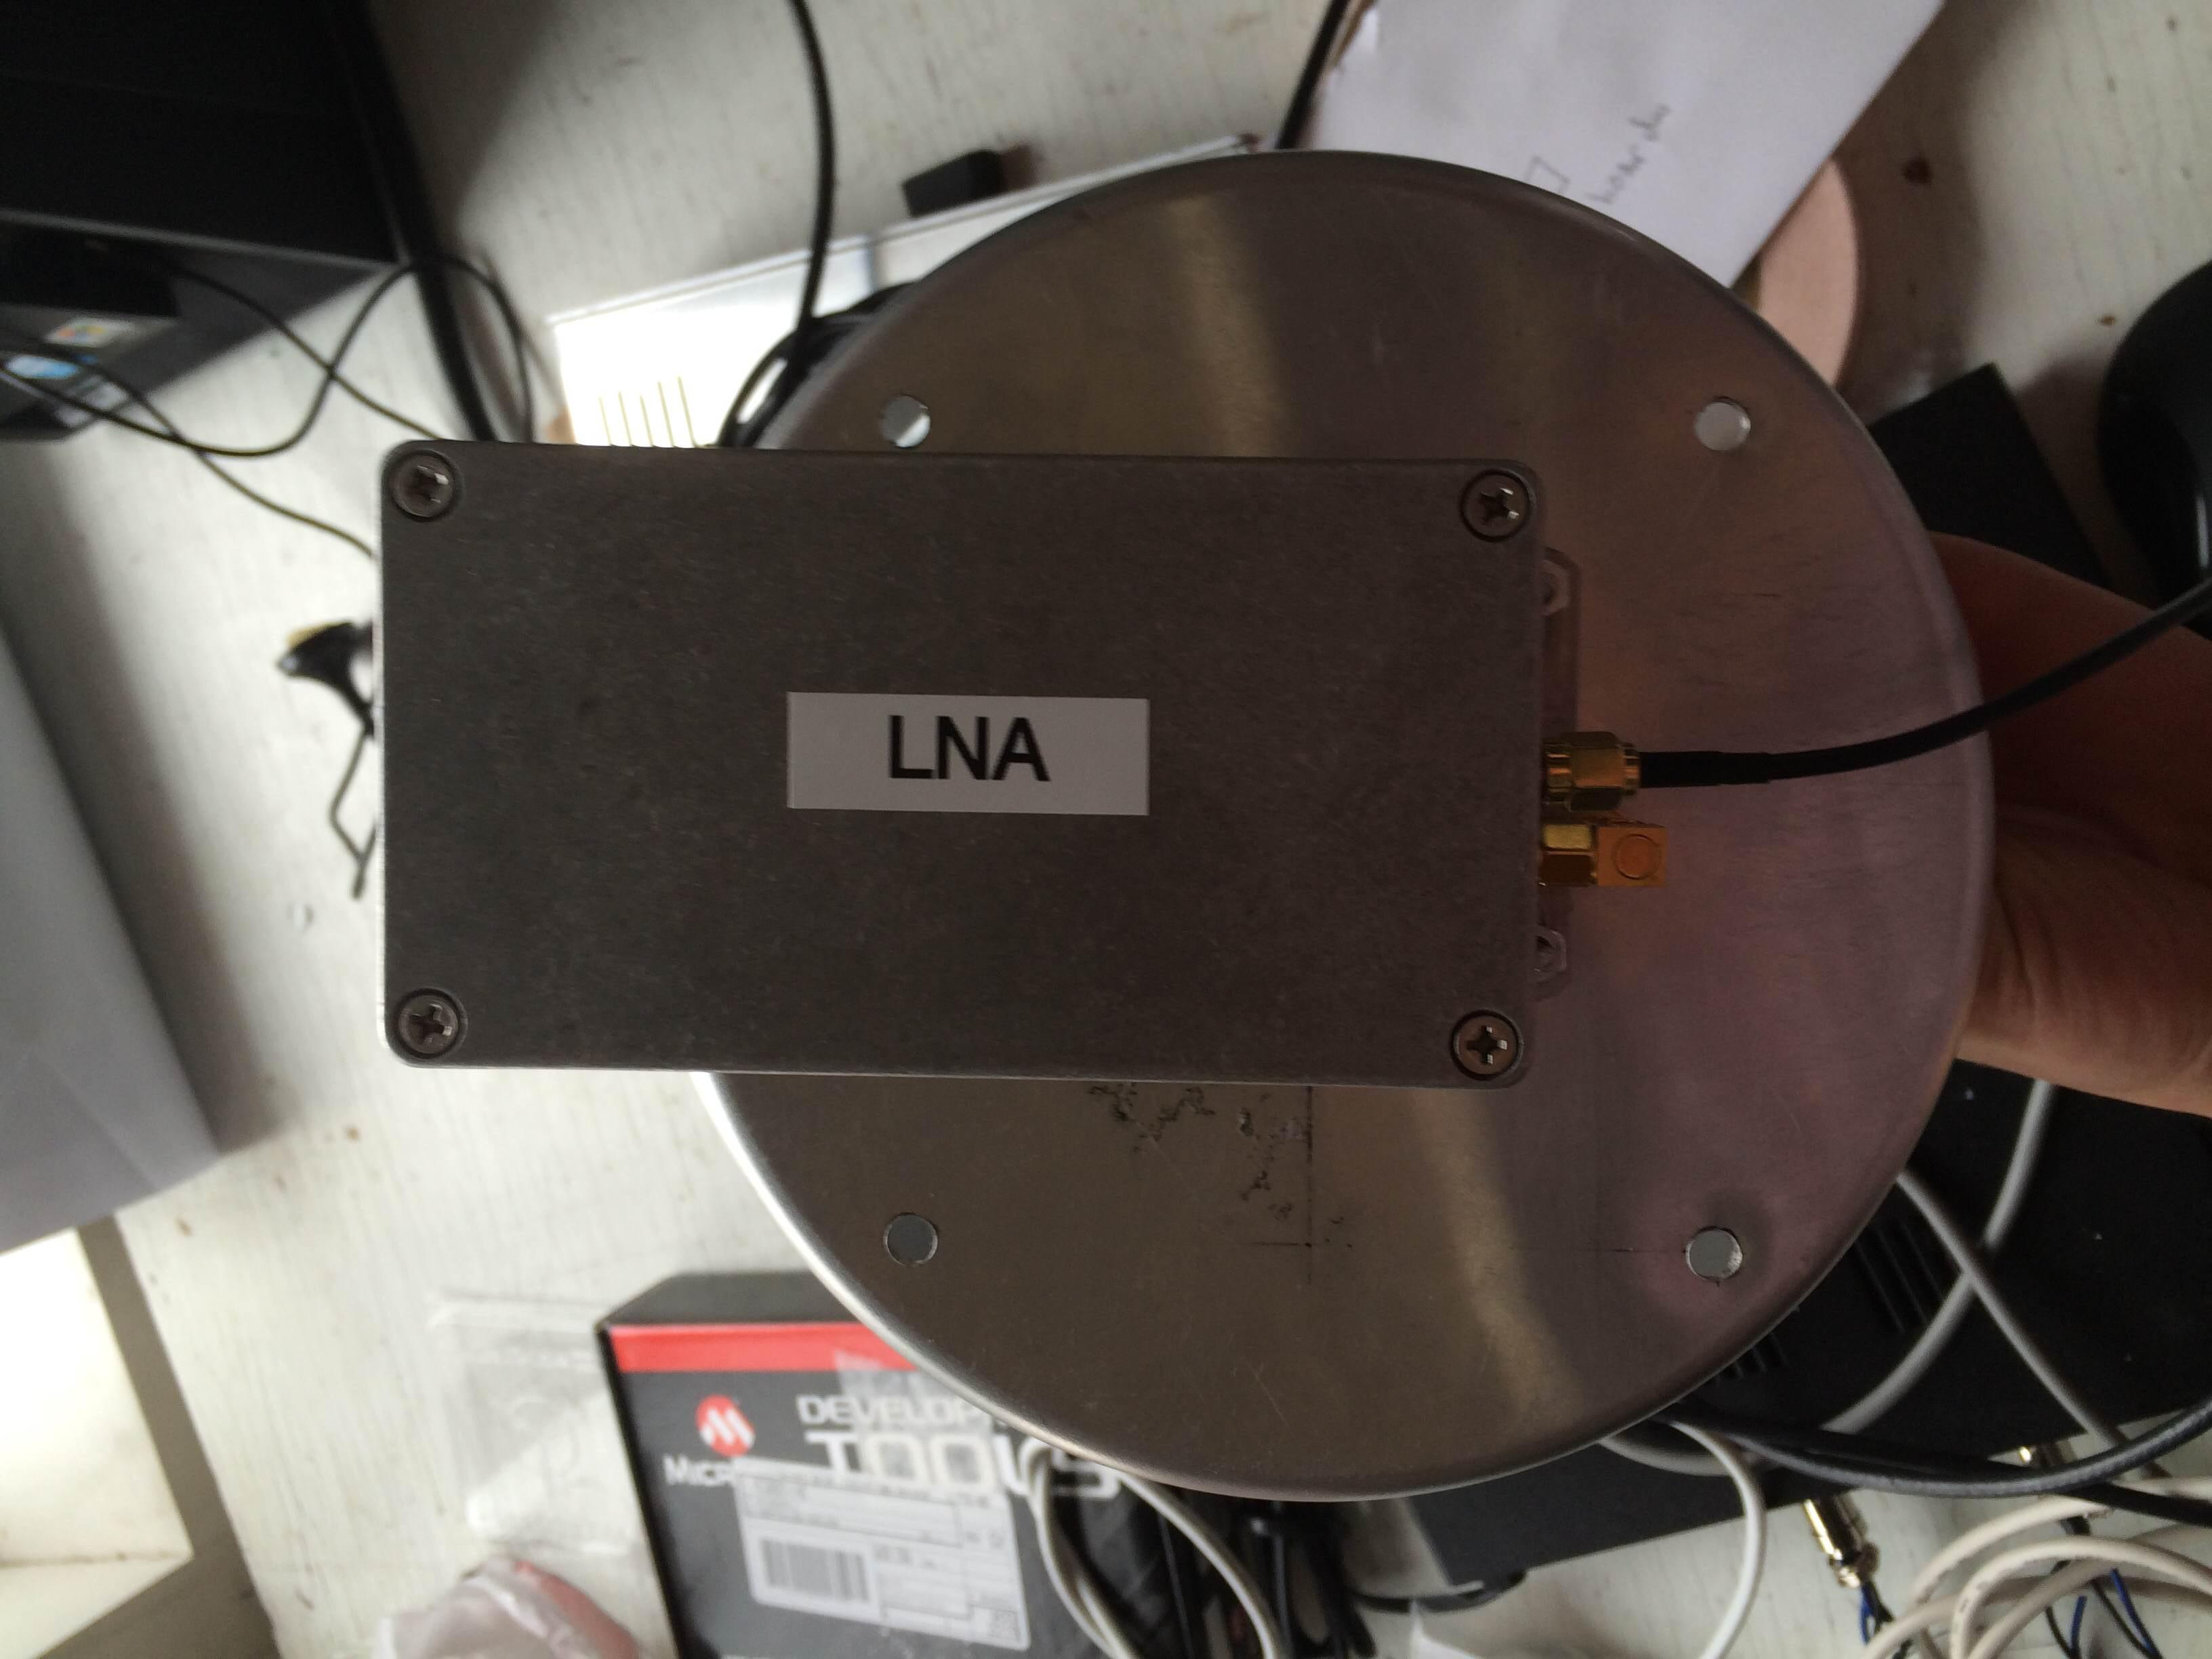
\includegraphics[scale=0.08]{feed/19.jpeg}
\end{center}

\begin{center}
\includegraphics[scale=0.08]{feed/20.jpeg}
\end{center}





%%%%%%%%%%%%%%%%%%%%%%%%%%%%%%%%%%%%%%%%

\subsection{Roof Mount}

\begin{center}
\includegraphics[scale=0.12]{roofmount/00.jpeg}
\end{center}

We used scrap metal to make our dish mount so we had to start by cleaning up the pieces of metal we were going to use and make them the right size.

We plasma cut a 1.5' x 3' rectangle of 5 gauge steel (about 3/16" thick, it later turned out this is to thin) and cleaned up the edges with a grinder.

\begin{center}
\includegraphics[scale=0.12]{roofmount/01.jpeg}
\end{center}

\begin{center}
\includegraphics[scale=0.12]{roofmount/02.jpeg}
\end{center}


We cut an 11.5' length of 2.5" (exterior diameter) pipe and cleaned in using a steel brush head on a grinder.

\begin{center}
\includegraphics[scale=0.12]{roofmount/03.jpeg}
\end{center}


We then MIG welded the pipe to the plate. We reinforced the weld with a couple extra beads because most of the force in the system will be directed to this point.

\begin{center}
\includegraphics[scale=0.12]{roofmount/04.jpeg}
\end{center}


The real trick was getting the pipe perpendicular to the plate.

\begin{center}
\includegraphics[scale=0.12]{roofmount/05.jpeg}
\end{center}


We ended up clamping the plate on one side of the table and then using the corner of the table as a perpendicular straight edge in two dimensions.

After some tests we realized the weight of the pipe was warping the plate so we successfully reinforced it with some angle iron.

\begin{center}
\includegraphics[scale=0.12]{roofmount/05.jpeg}
\end{center}

%%%%%%%%%%%%%%%%%%%%%%%%%%%%%%%%%%%%%%%%

\subsection{Dish}

We bolted together the central plates, trying to make sure they are parallel to each other.

Then we bolted on half of the dish arms which confirmed the accuracy of our central plate construction. This is as much of the dish as will fit out the door to the roof we will be mounting the dish on. The rest of the assembly happened on site.



\begin{center}
\includegraphics[scale=0.12]{dish/01.jpeg}
\end{center}

\begin{center}
\includegraphics[scale=0.12]{dish/02.jpeg}
\end{center}

\begin{center}
\includegraphics[scale=0.12]{dish/03.jpeg}
\end{center}

Once the ribs are put together and the support rings are in place, we are ready to put on the outer band.

\begin{center}
\includegraphics[scale=0.12]{dish/04.jpeg}
\end{center}

To do this, a hammer and tap were used to make dents in the end of the rib and the band

\begin{center}
\includegraphics[scale=0.12]{dish/05.jpeg}
\end{center}

Then, using a power drill, holes were cut in both so they could be lined up and riveted.

\begin{center}
\includegraphics[scale=0.12]{dish/06.jpeg}
\end{center}


This process of tapping, drilling, and riveting was repeated for each of the 12 ribs of the dish. Once complete, we were ready to start putting the mesh on.

Make sure all the ends of the support rings are together. We did not crimp them, since they seemed secure enough so that they would not fall out.

\begin{center}
\includegraphics[scale=0.12]{dish/07.jpeg}
\end{center}

Cutting the mesh!

Below are some pictures that detail the mesh cutting process.



\begin{center}
\includegraphics[scale=0.12]{dish/08.jpeg}
\end{center}

\begin{center}
\includegraphics[scale=0.12]{dish/09.jpeg}
\end{center}

\begin{center}
\includegraphics[scale=0.12]{dish/10.jpeg}
\end{center}

\begin{center}
\includegraphics[scale=0.12]{dish/11.jpeg}
\end{center}


After the Mesh was cut to specifications, it was laid out on the skeleton of the dish, to make sure there was enough material and it would come together properly

\begin{center}
\includegraphics[scale=0.12]{dish/12.jpeg}
\end{center}

After we were sure that we had enough material all cut to the right size to allow for some extra, all the sheets were removed except for one. One end of the sheet was secured to a rib using tape, while the other end was trimmed down to be flush with the next rib

\begin{center}
\includegraphics[scale=0.12]{dish/13.jpeg}
\end{center}

Then, the next sheet is placed on top of the end of the first sheet so they are overlapping, and a strip with pre-drilled holes (which came with the kit) were lined up on top of the rib, and holes were drilled through the rib at the places where the holes in the strip were

\begin{center}
\includegraphics[scale=0.12]{dish/14.jpeg}
\end{center}

The strip, with the overlapping pieces of mesh underneath, was then riveted to the rib.

\begin{center}
\includegraphics[scale=0.12]{dish/15.jpeg}
\end{center}


This process was repeated for all 12 sections of the dish until it was complete.

\begin{center}
\includegraphics[scale=0.12]{dish/16.jpeg}
\end{center}

Then, the edges were trimmed, leaving about 1/4 to 1/2 inch mesh past the outer band (enough to wrap around the band a bit)

\begin{center}
\includegraphics[scale=0.12]{dish/17.jpeg}
\end{center}

It was then wrapped around the band

\begin{center}
\includegraphics[scale=0.12]{dish/18.jpeg}
\end{center}


And secured using zipties (~ 4 zipties per section * 12 sections = ~ 48 zipties)


\begin{center}
\includegraphics[scale=0.12]{dish/19.jpeg}
\end{center}

\end{document}
